% Options for packages loaded elsewhere
\PassOptionsToPackage{unicode}{hyperref}
\PassOptionsToPackage{hyphens}{url}
%
\documentclass[
  12pt,
]{article}
\usepackage{lmodern}
\usepackage{amssymb,amsmath}
\usepackage{ifxetex,ifluatex}
\ifnum 0\ifxetex 1\fi\ifluatex 1\fi=0 % if pdftex
  \usepackage[T1]{fontenc}
  \usepackage[utf8]{inputenc}
  \usepackage{textcomp} % provide euro and other symbols
\else % if luatex or xetex
  \usepackage{unicode-math}
  \defaultfontfeatures{Scale=MatchLowercase}
  \defaultfontfeatures[\rmfamily]{Ligatures=TeX,Scale=1}
\fi
% Use upquote if available, for straight quotes in verbatim environments
\IfFileExists{upquote.sty}{\usepackage{upquote}}{}
\IfFileExists{microtype.sty}{% use microtype if available
  \usepackage[]{microtype}
  \UseMicrotypeSet[protrusion]{basicmath} % disable protrusion for tt fonts
}{}
\makeatletter
\@ifundefined{KOMAClassName}{% if non-KOMA class
  \IfFileExists{parskip.sty}{%
    \usepackage{parskip}
  }{% else
    \setlength{\parindent}{0pt}
    \setlength{\parskip}{6pt plus 2pt minus 1pt}}
}{% if KOMA class
  \KOMAoptions{parskip=half}}
\makeatother
\usepackage{xcolor}
\IfFileExists{xurl.sty}{\usepackage{xurl}}{} % add URL line breaks if available
\IfFileExists{bookmark.sty}{\usepackage{bookmark}}{\usepackage{hyperref}}
\hypersetup{
  pdftitle={TA Session of Econometrics 2 (2020-2021)},
  pdfauthor={Hiroki Kato; Pang Kan},
  hidelinks,
  pdfcreator={LaTeX via pandoc}}
\urlstyle{same} % disable monospaced font for URLs
\usepackage[margin=1in]{geometry}
\usepackage{color}
\usepackage{fancyvrb}
\newcommand{\VerbBar}{|}
\newcommand{\VERB}{\Verb[commandchars=\\\{\}]}
\DefineVerbatimEnvironment{Highlighting}{Verbatim}{commandchars=\\\{\}}
% Add ',fontsize=\small' for more characters per line
\usepackage{framed}
\definecolor{shadecolor}{RGB}{248,248,248}
\newenvironment{Shaded}{\begin{snugshade}}{\end{snugshade}}
\newcommand{\AlertTok}[1]{\textcolor[rgb]{0.94,0.16,0.16}{#1}}
\newcommand{\AnnotationTok}[1]{\textcolor[rgb]{0.56,0.35,0.01}{\textbf{\textit{#1}}}}
\newcommand{\AttributeTok}[1]{\textcolor[rgb]{0.77,0.63,0.00}{#1}}
\newcommand{\BaseNTok}[1]{\textcolor[rgb]{0.00,0.00,0.81}{#1}}
\newcommand{\BuiltInTok}[1]{#1}
\newcommand{\CharTok}[1]{\textcolor[rgb]{0.31,0.60,0.02}{#1}}
\newcommand{\CommentTok}[1]{\textcolor[rgb]{0.56,0.35,0.01}{\textit{#1}}}
\newcommand{\CommentVarTok}[1]{\textcolor[rgb]{0.56,0.35,0.01}{\textbf{\textit{#1}}}}
\newcommand{\ConstantTok}[1]{\textcolor[rgb]{0.00,0.00,0.00}{#1}}
\newcommand{\ControlFlowTok}[1]{\textcolor[rgb]{0.13,0.29,0.53}{\textbf{#1}}}
\newcommand{\DataTypeTok}[1]{\textcolor[rgb]{0.13,0.29,0.53}{#1}}
\newcommand{\DecValTok}[1]{\textcolor[rgb]{0.00,0.00,0.81}{#1}}
\newcommand{\DocumentationTok}[1]{\textcolor[rgb]{0.56,0.35,0.01}{\textbf{\textit{#1}}}}
\newcommand{\ErrorTok}[1]{\textcolor[rgb]{0.64,0.00,0.00}{\textbf{#1}}}
\newcommand{\ExtensionTok}[1]{#1}
\newcommand{\FloatTok}[1]{\textcolor[rgb]{0.00,0.00,0.81}{#1}}
\newcommand{\FunctionTok}[1]{\textcolor[rgb]{0.00,0.00,0.00}{#1}}
\newcommand{\ImportTok}[1]{#1}
\newcommand{\InformationTok}[1]{\textcolor[rgb]{0.56,0.35,0.01}{\textbf{\textit{#1}}}}
\newcommand{\KeywordTok}[1]{\textcolor[rgb]{0.13,0.29,0.53}{\textbf{#1}}}
\newcommand{\NormalTok}[1]{#1}
\newcommand{\OperatorTok}[1]{\textcolor[rgb]{0.81,0.36,0.00}{\textbf{#1}}}
\newcommand{\OtherTok}[1]{\textcolor[rgb]{0.56,0.35,0.01}{#1}}
\newcommand{\PreprocessorTok}[1]{\textcolor[rgb]{0.56,0.35,0.01}{\textit{#1}}}
\newcommand{\RegionMarkerTok}[1]{#1}
\newcommand{\SpecialCharTok}[1]{\textcolor[rgb]{0.00,0.00,0.00}{#1}}
\newcommand{\SpecialStringTok}[1]{\textcolor[rgb]{0.31,0.60,0.02}{#1}}
\newcommand{\StringTok}[1]{\textcolor[rgb]{0.31,0.60,0.02}{#1}}
\newcommand{\VariableTok}[1]{\textcolor[rgb]{0.00,0.00,0.00}{#1}}
\newcommand{\VerbatimStringTok}[1]{\textcolor[rgb]{0.31,0.60,0.02}{#1}}
\newcommand{\WarningTok}[1]{\textcolor[rgb]{0.56,0.35,0.01}{\textbf{\textit{#1}}}}
\usepackage{longtable,booktabs}
% Correct order of tables after \paragraph or \subparagraph
\usepackage{etoolbox}
\makeatletter
\patchcmd\longtable{\par}{\if@noskipsec\mbox{}\fi\par}{}{}
\makeatother
% Allow footnotes in longtable head/foot
\IfFileExists{footnotehyper.sty}{\usepackage{footnotehyper}}{\usepackage{footnote}}
\makesavenoteenv{longtable}
\usepackage{graphicx}
\makeatletter
\def\maxwidth{\ifdim\Gin@nat@width>\linewidth\linewidth\else\Gin@nat@width\fi}
\def\maxheight{\ifdim\Gin@nat@height>\textheight\textheight\else\Gin@nat@height\fi}
\makeatother
% Scale images if necessary, so that they will not overflow the page
% margins by default, and it is still possible to overwrite the defaults
% using explicit options in \includegraphics[width, height, ...]{}
\setkeys{Gin}{width=\maxwidth,height=\maxheight,keepaspectratio}
% Set default figure placement to htbp
\makeatletter
\def\fps@figure{htbp}
\makeatother
\setlength{\emergencystretch}{3em} % prevent overfull lines
\providecommand{\tightlist}{%
  \setlength{\itemsep}{0pt}\setlength{\parskip}{0pt}}
\setcounter{secnumdepth}{5}
\usepackage{ascmac}
\usepackage{zxjatype}
\setCJKmainfont[BoldFont = IPAゴシック]{IPA明朝}
\setCJKsansfont{IPAゴシック}
\setCJKmonofont{IPAゴシック}
\parindent = 1em
\newcommand{\argmax}{\mathop{\rm arg~max}\limits}
\newcommand{\argmin}{\mathop{\rm arg~min}\limits}
\DeclareMathOperator*{\plim}{plim}
\usepackage{xcolor}
\ifluatex
  \usepackage{selnolig}  % disable illegal ligatures
\fi
\newlength{\cslhangindent}
\setlength{\cslhangindent}{1.5em}
\newenvironment{cslreferences}%
  {\setlength{\parindent}{0pt}%
  \everypar{\setlength{\hangindent}{\cslhangindent}}\ignorespaces}%
  {\par}

\title{TA Session of Econometrics 2 (2020-2021)}
\author{Hiroki Kato \and Pang Kan}
\date{}

\begin{document}
\maketitle

{
\setcounter{tocdepth}{2}
\tableofcontents
}
\hypertarget{about-ta-session}{%
\section{About TA Session}\label{about-ta-session}}

\begin{itemize}
\tightlist
\item
  Class schedule: Friday pm 13:30-15:00 via zoom.

  \begin{itemize}
  \tightlist
  \item
    You can access the meeting ID and its pascode via CLE.
  \end{itemize}
\item
  Instructor (If you have any question, please contact us via e-mail)

  \begin{enumerate}
  \def\labelenumi{\arabic{enumi}.}
  \tightlist
  \item
    Hiroki Kato (D2, \href{mailto:vge008kh@student.econ.osaka-u.ac.jp}{\nolinkurl{vge008kh@student.econ.osaka-u.ac.jp}})
  \item
    Pang Kan (D1, \href{mailto:member_1363710747@yahoo.co.jp}{\nolinkurl{member\_1363710747@yahoo.co.jp}})
  \end{enumerate}
\item
  Purpose: We will review the contents of the main class ``Econometics II." using R which is a free software environment for statistical computing.

  \begin{itemize}
  \tightlist
  \item
    We strongly recommend that you download R (\url{https://www.r-project.org/}) and its IDE called R studio (\url{https://rstudio.com/products/rstudio/download/}), and try to reproduct by yourself.
  \end{itemize}
\end{itemize}

\hypertarget{reviews-of-matrix-algebra-and-probability}{%
\section{Reviews of Matrix Algebra and Probability}\label{reviews-of-matrix-algebra-and-probability}}

\hypertarget{matrix-algebra}{%
\subsection{Matrix Algebra}\label{matrix-algebra}}

\hypertarget{addition-and-subtraction}{%
\subsubsection{Addition and Subtraction}\label{addition-and-subtraction}}

Consider \(A = (a_{ij}) \in \mathbb{R}^{m \times n}\) and \(B = (b_{ij}) \in \mathbb{R}^{p \times q}\).
Addition and subtraction require that the dimentions are same, that is, \(m = p\) and \(n = q\).
Then, the sum of two matricies is
\begin{align*}
  A + B = (a_{ij} + b_{ij}).
\end{align*}
The difference of two matricies is
\begin{align*}
  A - B = (a_{ij} - b_{ij}).
\end{align*}

\hypertarget{multiplication}{%
\subsubsection{Multiplication}\label{multiplication}}

The standard matrix multiplication requires that
the number of columns of the first matrix is equal to the number of rows of the second matrix (\(n = p = l\)).
The product of two matricies is
\begin{align*}
  AB = (\sum_{k=1}^l a_{ik} b_{kj}) \in \mathbb{R}^{m \times q}.
\end{align*}
We should remark following important points about multiplication:

\begin{itemize}
\tightlist
\item
  it holds non-commutativity: \(XY \not= YX\);
\item
  it holds associative law: \((XY)Z = X(YZ)\);
\item
  it holds distributive law: \(X(Y + Z) = XY + XZ\);
\item
  when \(B = A\), we obtain the second power of a matrix \(A\), that is, \(A^2 = A A\). Especially, if a martix \(A\) holds \(AA = A\), then the matrix is called an \textbf{idempotent matrix (べき等行列)}.
\end{itemize}

We introduce the another key product of matrix, called the \textbf{Kronecker product (クロネッカー積)}.
This is defined by
\begin{align*}
  A \otimes B = (a_{ij} B) \in \mathbb{R}^{mp \times nq}.
\end{align*}
The Kronecker product has a following property:

\begin{itemize}
\tightlist
\item
  \(X_{1}X_{2} \otimes Y_{1}Y_{2} = (X_{1} \otimes Y_{1})(X_{2} \otimes Y_{2})\)
\end{itemize}

\hypertarget{transposed-matrix-diagonal-matrix-and-inverse-matrix}{%
\subsubsection{Transposed Matrix, Diagonal Matrix, and Inverse Matrix}\label{transposed-matrix-diagonal-matrix-and-inverse-matrix}}

Consider \(X = (x_{ij}) \in \mathbb{R}^{m \times n}\) throughout this subsection.

\hypertarget{transposed-matrix}{%
\paragraph{Transposed Matrix}\label{transposed-matrix}}

The \textbf{transposed matrix (転置行列)} of \(X\), denoted by \(X'\) is a \(n \times m\) matrix whose element \(x'_{ij}\) holds
\begin{align*}
  x'_{ij} = x_{ji}.
\end{align*}
That is, \(i\)-th row and \(j\)-th column element of transposed matrix is
\(j\)-th row and \(i\)-th column element of original matrix.
We remark following important points:

\begin{itemize}
\tightlist
\item
  it holds \((XY)' = Y'X'\);
\item
  it holds \((XYZ)' = Z'Y'X'\);
\item
  \((X \otimes Y)' = X' \otimes Y'\);
\item
  let \(x_i = (x_{i1}, \ldots x_{ij})\) be a row vector of matrix \(X\). Then, we have \(X'X = \sum_{n = 1}^i x'_n x_n\);
\item
  if a matrix \(X\) holds \(X' = X\), then the matrix is called a \textbf{symmetric matrix (対称行列)}.
\end{itemize}

\hypertarget{diagonal-matrix-and-trace}{%
\paragraph{Diagonal Matrix and Trace}\label{diagonal-matrix-and-trace}}

Suppose a matrix \(X\) is a \textbf{square matrix (正方行列)}, that is, \(n = m\).
The matrix \(X\) is called a \textbf{diagonal matrix (対角行列)}
whose diagonal elements (\(i\)-th row and \(i\)-th column elements) consist of \((x_{11}, \ldots x_{nn})\),
and other elements are zero.
That is,
\begin{align*}
  X 
  = diag(x_{11}, x_{22}, \ldots, x_{ii})
  =
  \begin{pmatrix}
    x_{11} & 0 & 0 & \cdots & 0 \\
    0 & x_{22} & 0 & \cdots & 0 \\
    \vdots & \vdots & \vdots & \vdots & \vdots \\
    0 & 0 & 0 & \cdots & x_{nn}
  \end{pmatrix}.
\end{align*}
Especially, a matrix \(I = diag(1, 1, \ldots, 1)\) is called an \textbf{identity matrix (単位行列)}.

There is one important concept, called \textbf{trace (トレース)}, related with diagonal elements of matrix.
The trace of matrix is derived by the sum of diagonal elements, that is,
\begin{align*}
  tr(X) = \sum_{n = 1}^{i} x_{nn}.
\end{align*}
The trace has following properties:

\begin{itemize}
\tightlist
\item
  \(tr(cX) = c \cdot tr(X)\) where \(c\) is scalar;
\item
  \(tr(X') = tr(X)\);
\item
  \(tr(X + Y) = tr(X) + tr(Y)\);
\item
  \(tr(XY) = tr(YX)\);
\item
  \(xx' = tr(x'x) = tr(x x')\) if \(x\) is a \(1 \times j\) vector.
\end{itemize}

\hypertarget{inverse-matrix}{%
\paragraph{Inverse Matrix}\label{inverse-matrix}}

the matrix \(X\) is \textbf{regular matrix (正則行列)} if there exists a matrix \(Y\) such that
\begin{align*}
  X Y = I,
\end{align*}
where \(I\) is an identity matrix.
In this case, the matrix \(Y\) is called an \textbf{inverse matrix (逆行列)}, which is denoted by \(X^{-1}\).
The inverse matrix has following important properties:

\begin{itemize}
\tightlist
\item
  \((X^{-1})' = (X')^{-1}\);
\item
  \((X \otimes Y)^{-1} = X^{-1} \otimes Y^{-1}\) if the inverse exists;
\item
  \((X \otimes Y)(X^{-1} \otimes Y^{-1}) = I\)
\end{itemize}

\hypertarget{quadratic-forms}{%
\subsubsection{Quadratic Forms}\label{quadratic-forms}}

Consider a symmetric and square matrix \(A \in \mathbb{R}^{n \times n}\) and a vector \(x \in \mathbb{R}^{n \times 1}\).
Then, the quadratic form is written as
\begin{align*}
  Q = x' A x.
\end{align*}
For example, consider \(x = (x, y)'\) and \(A\) is a \(2 \times 2\) matrix whose elements is one.
Then, the quadratic form is
\begin{align*}
  Q 
  =
  \begin{pmatrix} x & y \end{pmatrix}
  \begin{pmatrix} 1 & 1 \\ 1 & 1 \end{pmatrix}
  \begin{pmatrix} x \\ y \end{pmatrix}
  =
  \begin{pmatrix} x+y & x+y \end{pmatrix}
  \begin{pmatrix} x \\ y \end{pmatrix}  
  = x^2 + 2xy + y^2 = (x + y)^2.
\end{align*}
In this case, for any non-zero \(x\) and \(y\), \(Q\) takes non-negative value.
Then, we call the matrix \(A\) \emph{positive semidefinite}.
The definiteness of matrix is defined as follows:

\begin{itemize}
\tightlist
\item
  If \(x'Ax > 0\) for all nonzero \(x\), then \(A\) is \textbf{positive definite (正値定符号)}.
\item
  If \(x'Ax < 0\) for all nonzero \(x\), then \(A\) is \textbf{negative definite (負値定符号)}.
\item
  If \(x'Ax \ge 0\) for all nonzero \(x\), then \(A\) is \textbf{positive semidefinite (半正値定符号)}.
\item
  If \(x'Ax \le 0\) for all nonzero \(x\), then \(A\) is \textbf{negative semidefinite(半負値定符号)}.
\end{itemize}

\hypertarget{characteristic-roots-and-characteristic-vectors}{%
\paragraph{Characteristic Roots and Characteristic Vectors}\label{characteristic-roots-and-characteristic-vectors}}

Before describing useful theorm to check definiteness easily,
we have to introduce two concepts: \textbf{characteristic roots (固有根)} and \textbf{characteristic vectors (固有ベクトル)}.

\begin{quote}
If a scalar \(\lambda\) and a vector \(c\in \mathbb{R}^{k \times 1}\), which is normalized as \(c'c=1\), satisfy the following equation, then they are called as the \textbf{characteristic root} and the \textbf{characteristic vector}, respectively;
\begin{align*}
Ac=\lambda c \Leftrightarrow (A-\lambda I)c = 0,
\end{align*}
where \(I\) is an identity matrix.
\end{quote}

These (\(\lambda_1,\lambda _2,...,\lambda _k\)) correspond to characteristic vectors \((c_1, c_2, \dots ,c_k)\).
There is the following useful theorm that states the relationship between characteristic roots and definiteness:

\begin{quote}
Let \(A\) be a symmetric matrix.

\begin{enumerate}
\def\labelenumi{\arabic{enumi}.}
\tightlist
\item
  If all the characteristic roots of \(A\) are positive (negative), then \(A\) is positive definite (negative definite).
\item
  If some of roots are zero, then \(A\) is positive (negative) semidefinite if the reminder are positive (negative).
\item
  If \(A\) has both negative and positive roots, then \(A\) is indefinite.
\end{enumerate}
\end{quote}

\hypertarget{determinants}{%
\paragraph{Determinants}\label{determinants}}

Alternative way to check definiteness of matrix is to using \textbf{determinants (行列式)},
which is a scalar quantity defined by a square matrix \(A = (a_{ij}) \in \mathbb{R}^{n \times n}\).
The determinant of \(2 \times 2\) matrix, i.e., \(n = 2\), is obtained by
\begin{align*}
  det(A) = a_{11}a_{22} - a_{12}a_{21}.
\end{align*}
Using the determinant of a matrix with \(n = 2\), we can calculate the determinant of \(3 \times 3\) matrix.
Let \(det(A_{ij})\) be the determinant of the \(2 \times 2\) submatrix
obtained when \(i\)-th row and \(j\)-th column are removed from the original matrix,
which is called \textbf{minor (小行列式)}.
Furthermore, we define \(C_{ij} = (-1)^{i+j} det(A_{ij})\), which is called \textbf{cofactor (余因子)}.
We call a matrix in which each element \(a_{ij}\) is replaced by the corresponding cofactor \(C_{ij}\) \textbf{cofactor matrix (余因子行列)}.
Then, the determinant of \(3 \times 3\) matrix is
\begin{align*}
  det(A) 
  &= a_{11} C_{11} + a_{12} C_{12} + a_{13} C_{13}  \\
  &= a_{11} 
  \left| \begin{array}{cc}
    a_{22} & a_{23} \\
    a_{32} & a_{33}
  \end{array} \right| 
  - a_{12}
  \left| \begin{array}{cc}
    a_{21} & a_{23} \\
    a_{31} & a_{33}
  \end{array} \right| 
  + a_{13}
  \left| \begin{array}{cc}
    a_{21} & a_{22} \\
    a_{31} & a_{32}
  \end{array} \right|, 
\end{align*}
or
\begin{align*}
  det(A) = a_{11} C_{11} + a_{21} C_{21} + a_{31} C_{31}.
\end{align*}
How about matrices with \(n \ge 4\)?
Essentially, we can calculate the determinant, using cofactors. That is, for any \(i\),
\begin{align*}
  det(A) = \sum_{k = 1}^n a_{ik} C_{ik},
\end{align*}
or, for any \(j\)
\begin{align*}
  det(A) = \sum_{k = 1}^n a_{kj} C_{kj},
\end{align*}

Before describing the important theorem to check definiteness,
we introduce the \emph{Cramer's rule}, which provides inverse matrices.

\begin{quote}
Let \(A \in \mathbb{R}^{n \times n}\) be a square matrix with \(det(A) \not= 0\).
Then, the inverse matrix of \(A\) is equal to the transposed cofactor matrix multiplied by \(det(A)^{-1}\). That is,
\begin{align*}
A^{-1} = \frac{1}{det(A)} 
\begin{pmatrix}
C_{11} & \cdots & C_{n1} \\
\vdots & \vdots & \vdots \\
C_{1n} & \cdots & C_{nn}
\end{pmatrix}. 
\end{align*}
\end{quote}

Next, we introduce the useful theorem to check definiteness of matricies.
The determinant has the follwoing relation with the definiteness of matricies.

\begin{quote}
Let \(A \in \mathbb{R}^{n \times n}\) be a square matrix. Let
\begin{align*}
det(A_i) = 
\left| \begin{array}{ccc}
a_{11} & \cdots & a_{1i} \\
\vdots & \vdots & \vdots \\
a_{i1} & \cdots & a_{ii}
\end{array} \right|. 
\end{align*}
A necessary and sufficient condition for a matrix A to be positive definite is that \(det(A_i) > 0\) for all \(i \in \{1, \ldots, n\}\).
Moreover, a necessary sufficient condition for a matrix A to be negative definite is
that \(det(A_i) < 0\) for odd \(i\) and \(det(A_i) > 0\) for even \(i\).
\end{quote}

As an illustration, consider the following matrix:
\begin{align*}
  A = 
  \begin{pmatrix}
    6 & 4 \\
    4 & 5
  \end{pmatrix}.
\end{align*}
Then, we have \(det(A_1) = 6 > 0\) and \(det(A_2) = 30 - 16 > 0\).
Thus, this matrix is positive definite.

To show another example, we use the following diagonal matrix:
\begin{align*}
  A = 
  \begin{pmatrix}
    -3 & 0 & 0 \\
    0 & -2 & 0 \\
    0 & 0 & -1
  \end{pmatrix}.
\end{align*}
Since the determinant of a diagonal matrix can be computed as the product of diagonal elements,
we have \(det(A_1) = -3\), \(det(A_2) = (-3)(-2) = 6 > 0\), and \(det(A_3) = (-3)(-2)(-1) = -6 < 0\).
Thus, this diagonal matrix is negative definite.
Moreover, the inverse matrix of this diagonal matrix is given by
\begin{align*}
  A^{-1} = -\frac{1}{6}
  \begin{pmatrix}
    2 & 0 & 0 \\
    0 & 3 & 0 \\
    0 & 0 & 6
  \end{pmatrix}
  = 
  \begin{pmatrix}
    -1/3 & 0 & 0 \\
    0 & -1/2 & \\
    0 & 0 & -1
  \end{pmatrix}
\end{align*}
Cleary, we have \(A A^{-1} = I\).

\hypertarget{differentiation}{%
\subsubsection{Differentiation}\label{differentiation}}

Consider two vectors: \(a \in \mathbb{R}^{n \times 1}\) and \(x \in \mathbb{R}^{n \times 1}\).
We obtain the product of transposed vector of \(a\) and \(x\), that is,
\(a'x = a_1 x_1 + \cdots + a_n x_n\).
Then, the differentiation of this scalar with respect to \(x\) is defined by
\begin{align*}
  \frac{\partial a'x}{\partial x}
  = 
  \begin{pmatrix} \frac{\partial a'x}{\partial x_1} \\ \vdots \\ \frac{\partial a'x}{\partial x_n} \end{pmatrix}
  = 
  a.
\end{align*}

Now, we expand to a symmetric and square matrix \(A \in \mathbb{R}^{n \times n}\).
Then, the differentiation of the quadratic form \(x' A x\) with respect to \(x\) is defined by
\begin{align*}
  \frac{\partial x'Ax}{\partial x} = (A + A')x.
\end{align*}

\hypertarget{optimization}{%
\paragraph{Optimization}\label{optimization}}

Consider function \(y = g(x)\) where \(x \in \mathbb{R}^{n}\), denoted as \(g: \mathbb{R}^{n} \to \mathbb{R}\).
We can obtain \(x^0\) such that maximizing (minimizing) the function \(g\), using the following theorem:

\begin{quote}
If a function \(g \colon \mathbb{R}^{n} \rightarrow \mathbb{R}\) is maximized (minimized) at the point \(x^{0} = (x_{1}^{0}, \ldots, x_{n}^{0})\), then the following equation holds:
\begin{align*}
\frac{\partial g (x)}{\partial x} \Big{\vert}_{x = x^{0}} 
= 
\begin{pmatrix}
\frac{\partial g (x^{0})}{\partial x_{1}} \\
\vdots \\
\frac{\partial g (x^{0})}{\partial x_{n}} 
\end{pmatrix}  
= 0.
\end{align*}
\(x^0\) is maximum (minimum) point if the following \textbf{Hessian matrix (ヘッセ行列)} is negative (positive) definite:
\begin{align*}
H = \frac{\partial g (x)}{\partial xx'} 
=
\begin{pmatrix}
\frac{\partial^{2} g (x)}{\partial x_{1} \partial x_{1}} 
& \cdots & \frac{\partial^{2} g (x)}{\partial x_{1} \partial x_{n}} \\
\vdots  &\ddots  &\vdots\\
\frac{\partial^{2} g (x)}{\partial x_{n} \partial x_{1}} 
& \cdots & \frac{\partial^{2} g (x)}{\partial x_{n} \partial x_{n}}
\end{pmatrix}.
\end{align*}
\end{quote}

\hypertarget{probability}{%
\subsection{Probability}\label{probability}}

This section refers to Wasserman (2013).
Let \(\Omega\) be a \textbf{(sample) space} which is the set of possible outcomes of an experiment.
Let \(\omega\) be \textbf{sample outcomes}, \textbf{reaizations}, or \textbf{elements}.
Let \(A\) be \textbf{events} which are the subsets of \(\Omega\).
Then, we can define the \textbf{probability} and \textbf{random variable} as follows:

\begin{quote}
A function \(\mathbb{P}\) that assigns a real number \(\mathbb{P}(A)\) to each event A is a \textbf{probability} if it satisfies the following three axioms:

\begin{enumerate}
\def\labelenumi{\arabic{enumi}.}
\tightlist
\item
  \(\mathbb{P}(A) \ge 0\) for all \(A\);
\item
  \(\mathbb{P}(\Omega) = 1\);
\item
  If \(A_1, A_2, \ldots\) are disjoint, then \(\mathbb{P}(\bigcup_{k=1}^{\infty}{A_k}) = \sum_{k=1}^{\infty} \mathbb{P}(A_i)\).
\end{enumerate}

A \textbf{random variable} is a mapping \(X: \Omega \to \mathbb{R}\) that assigns a real number \(X(\omega)\) to each realization \(\omega\).
\end{quote}

For illustlation, consider the situation where you try to flip a fair coin twice.
Then, the sample space \(\Omega = \{ TT, HH, TH, HT \}\).
The probability of each outcome is 1/4, that is, \(P(\omega) = 1/4\) for all \(\omega\).
Let the random variable \(X\) be the number of heads.
Then, \(X(TT) = 0\), \(X(HH) = 2\), \(X(TH) = 1\), and \(X(HT) = 1\).

\hypertarget{distribution-functions}{%
\subsubsection{Distribution Functions}\label{distribution-functions}}

Given a random variable \(X\), we define \textbf{probability mass function}, \textbf{probability density function} and \textbf{cumulative distribution function} as follows:

\begin{quote}
Suppose that a random variable \(X\) is \emph{discrete} taking countably many values \(\{x_1, \ldots\}\). Then, the \textbf{probability mass function} for \(X\) is defined by \(f_X(x) = \mathbb{P}(X = x)\).

Suppose that a random variable \(X\) is \emph{continuous}. Then, there exists a \textbf{probability density function} \(f_X\) such that (i) \(f_X(x) \ge 0\) for all x, (ii) \(\int_{-\infty}^{+\infty} f_X(x) dx = 1\) and (iii) for every \(a \le b\), \(\mathbb{P}(a < X < b) = \int_a^b f_X(x)dx\).

The \textbf{cumulative distribution function (CDF)} is the function \(F_X: \mathbb{R} \to [0, 1]\) defined by \(F_X(x) = \mathbb{P}(X \le x)\).
\end{quote}

We summarize the relationship among three distribution functions as follows:
\begin{align*}
  F_X(x) =
  \begin{cases}
    \sum_{x_i \le x} f_X(x_i)  &\quad\text{$X$ is discrete} \\
    \int_{-\infty}^x f_X(t)dt  &\quad\text{$X$ is continuous}
  \end{cases}
\end{align*}
From this, we obtain the property of CDF:

\begin{itemize}
\tightlist
\item
  \(F\) is non-decreasing: \(x_1 < x_2\) implies \(F(x_1) \le F(x_2)\);
\item
  \(F\) is normalized: \(\lim_{x \to -\infty} F(x) = 0\) and \(\lim_{x \to +\infty} F(x) = 1\);
\item
  \(F\) is right-contious: \(F(x) = F(x^+)\) for all \(x\), where \(F(x^+) = \lim_{y \downarrow x} F(y)\);
\item
  \(\mathbb{P}(X = x) = F(x) - F(x^-)\) where \(F(x^-) = \lim_{y \uparrow x} F(y)\);
\item
  \(\mathbb{P}(x < X \le y) = F(y) - F(x)\);
\item
  \(\mathbb{P}(X > x) = 1 - F(x)\).
\end{itemize}

\hypertarget{bivariate-distributions}{%
\paragraph{Bivariate Distributions}\label{bivariate-distributions}}

When there are two random varibales, you can define bivariate distributions as follows:

\begin{quote}
Given discrete random variables \(X\) and \(Y\), we define the \textbf{joint mass function} by \(f_{X,Y}(x, y) = \mathbb{P}(X = x, Y = y)\).
\end{quote}

\begin{quote}
In the continuous case, we call a function \(f(x, y)\) a \textbf{joint probability density function} for the random variables \((X, Y)\) if (i) \(f(x, y) \ge 0\), \(\forall (x, y)\), (ii) \(\int_{-\infty}^{+\infty} \int_{-\infty}^{+\infty} f(x, y)dx dy = 1\), and, (iii) for any \(A \subset \mathbb{R} \times \mathbb{R}\), \(\mathbb{P}[(X, Y) \in A] = \int \int_A f(x, y)dx dy\).
\end{quote}

\begin{quote}
In both cases, we define the \textbf{joint cumulative distribution function} as \(F_{X,Y}(x, y) = \mathbb{P}(X \le x, Y \le y)\).
\end{quote}

When you are interested to the probability of a single event occurring,
there are two distributions called a \textbf{marginal distribution (周辺分布)} and a \textbf{conditional distribution (条件付き分布)}.
The formar distribution is the probability of \(X = x\) independent of \(Y\).
On the other hand,
the latter distribution is the probability that \(X = x\) occurs given the event \(Y = y\) has already occured.
Formally,

\begin{quote}
The \textbf{marginal distribution} is defined by
\begin{align*}
f_X(x) 
= 
\mathbb{P}(X = x)
=
\begin{cases}
\sum_y \mathbb{P}(X = x, Y = y)  &\quad\text{$X$ is discrete} \\
\int f(x, y) dy &\quad\text{$X$ is continuous}
\end{cases}.
\end{align*}
The \textbf{conditional distribution} is defined by
\begin{align*}
f_{X|Y}(x|y)
= 
\mathbb{P}(X = x | Y = y)
= 
\begin{cases}
\sum_y \frac{\mathbb{P}(X = x, Y = y)}{\mathbb{P}(Y = y)}  &\quad\text{$X$ is discrete} \\
\int \frac{f_{X,Y}(x, y)}{f_Y(y)} dy &\quad\text{$X$ is continuous}
\end{cases},
\end{align*}
\end{quote}

To define the conditional distribution function,
we assume \(\mathbb{P}(Y = y) > 0\) for discrete random variables and \(f_Y(y) > 0\) for continuous random variables.
In the case of continuous random variables, we must integrate to get a probability, that is,
\begin{align*}
  \mathbb{P}(X \in A | Y = y) = \int_A f_{X|Y}(x|y) dx.
\end{align*}

Finally, we introduce very important concept of probability, called \textbf{independence}, and define it as follows:

\begin{quote}
Two random variables \(X\) and \(Y\) are \textbf{independent} if, for every event \(A\) and \(B\), \(\mathbb{P}(X \in A, Y \in B) = \mathbb{P}(X \in A) \mathbb{P}(Y \in B)\).
\end{quote}

In principle, to check independence, we need to check whether this relationship for all subsets \(A\) and \(B\).
But, there is useful theorem to check independence.

\begin{quote}
Let \(X\) and \(Y\) have joint PDF \(f_{X,Y}\). Then, \(X\) and \(Y\) are independent if and only if \(f_{X,Y}(x,y) = f_X(x) f_Y(y)\) for all values \(x\) and \(y\).
\end{quote}

Note that if two random variables are independent,
then the conditional probability \(\mathbb{P}(X = x | Y = y)\) reduces to \(\mathbb{P}(X = x)\).

\hypertarget{expectations-variance-and-covariance}{%
\subsubsection{Expectations, Variance, and Covariance}\label{expectations-variance-and-covariance}}

Roughly speaking, the expectation of a random variable \(X\) is the average value of \(X\).
The variance of a random variable \(X\) measures the ``spread" of a distribution.
Formally,

\begin{quote}
The \textbf{expected value (mean, first moment)} of \(X\) is defined to be
\begin{align*}
E(X) 
= \mu_X
= \int x dF(x) 
=
\begin{cases}
\sum_x x f(x)  &\quad\text{$X$ is discrete}  \\
\int x f(x) dx &\quad\text{$X$ is continuous} 
\end{cases}
\end{align*}
The \textbf{variance} of \(X\) is defined by \(V(X) = \sigma^2 = E(X - \mu_X)^2 = \int (x - \mu_X)^2 dF(x)\). The \textbf{standard deviation} is \(sd(X) = \sqrt{V(X)}\).
\end{quote}

The mean of random variable, \(E(X)\), exists if \(\int_x |x| dF_X(x) < \infty\).
Expectation and variance has some useful properties:

\begin{itemize}
\tightlist
\item
  Let \(Y = r(X)\). Then, \(E(Y) = E(r(X)) = \int r(x) dF(x)\);
\item
  Suppose that \(X_1, \ldots, X_n\) are random variables and \(a_1, \ldots, a_n\) are constants. \(E(\sum_i a_i X_i) = \sum_i a_i E(X_i)\);
\item
  Suppose that \(X_1, \ldots, X_n\) are independent random variables. Then, \(E(\prod_{i=1}^n X_i) = \prod_i E(X_i)\);
\item
  \(V(X) = E(X^2) - \mu^2\);
\item
  \(V(aX + b) = a^2 V(X)\) where \(a\) and \(b\) are constants;
\item
  Suppose that \(X_1, \ldots, X_n\) are independent random variables and \(a_1, \ldots, a_n\) are constants. \(V(\sum_i a_i X_i) = \sum_i a_i^2 V(X_i)\).
\item
  If \(a\) is a vector and \(X\) is a random vector with mean \(\mu\) and variance \(\Sigma\), then \(E(a'X) = a'\mu\) and \(V(a'X) = a'\Sigma a\). If \(A\) is a matrix, then \(E(AX) = A\mu\) and \(V(AX) = A\Sigma A'\).
\end{itemize}

We introduce some theorems about probability inequalities which is used in the theory of convergence.

\begin{itemize}
\tightlist
\item
  Markov's inequality: Let \(X\) be a non-negative random variable and suppose that \(E(X)\) exists. For any \(t > 0\), \(\mathbb{P}(X > t) \le E(X)/t\).
\item
  Chebyshev's inequality: Let \(\mu = E(X)\) and \(\sigma^2 = V(X)\). Then, \(\mathbb{P}(|X - \mu| \ge t) \le \sigma^2/t^2\) and \(\mathbb{P}(|Z| \ge k) \le 1/k^2\) where \(Z = (X - \mu)/\sigma\).
\item
  Jensen's inequality: If \(g\) is convex, then \(E[ g(X) ] \ge g(E(X))\). If \(g\) is concave, then \(E[ g(X) ] \le g(E(X))\).
\end{itemize}

Next, we will introduce the definition of \textbf{covariance}. These measure how strong the linear relationship is between \(X\) and \(Y\).

\begin{quote}
Let \(X\) and \(Y\) be random variables with means \(\mu_X\) and \(\mu_Y\), respectively. Then, the \textbf{covariance} between \(X\) and \(Y\) is defined by \(\mathrm{Cov}(X, Y) = E[(X - \mu_X)(Y - \mu_Y)]\).
\end{quote}

Covariance has following properties:

\begin{itemize}
\tightlist
\item
  \(\mathrm{Cov}(X, Y) = E(XY) - E(X)E(Y)\);
\item
  If \(X\) and \(Y\) are independent, \(\mathrm{Cov}(X, Y) = 0\). \textbf{The converse is not true.}
\item
  \(V(X + Y) = V(X) + V(Y) + 2\mathrm{Cov}(X, Y)\)
\item
  \(V(X - Y) = V(X) + V(Y) - 2\mathrm{Cov}(X, Y)\)
\item
  \(V(\sum_i a_i X_i) = \sum_i a_i^2 V(X_i) + 2 \sum_i \sum_{i < j} a_i a_j \mathrm{Cov}(X_i, X_j)\).
\end{itemize}

\hypertarget{conditional-expectation-and-variance}{%
\paragraph{Conditional Expectation and Variance}\label{conditional-expectation-and-variance}}

\begin{quote}
The conditional expectation of \(X\) given \(Y = y\) is
\begin{align*}
E(X|Y = y)
=
\begin{cases}
\sum_x x f_{X|Y}(x|y) &\quad\text{$X$ is discrete}  \\
\int x f_{X|Y}(x|y) dx &\quad\text{$X$ is continuous}  \\
\end{cases}
\end{align*}
The conditional variance is defined as
\begin{align*}
V(X | Y = y) = \int (x - \mu(y))^2 f(x|y) dx.
\end{align*}
where \(\mu(y) = E(X | Y = y)\).
\end{quote}

Even if \(r(x, y)\) is a function of \(x\) and \(y\), we can define the conditional expectation.
For the continuous random variable, \(E[r(X, Y) | Y = y] = \int r(x, y) f_{X|Y}(x|y) dx\).
For the discrete random variable, \(E[r(X, Y) | Y = y] = \sum_x r(x, y) f_{X|Y}(x|y)\).

We have following important properties:

\begin{itemize}
\tightlist
\item
  For random variables \(X\) and \(Y\), assuming the expectations exist, we have that \(E_X[ E(Y|X) ] = E(Y)\). More generally, for any function \(r(x, y)\), we have \(E_X[ E(r(X, Y)|X) ] = E(r(X, Y))\).
\item
  For random variables \(X\) and \(Y\), \(V(Y) = E_X[ V(Y|X) ] + V_X[ E(Y|X) ]\).
\end{itemize}

\hypertarget{moment}{%
\paragraph{Moment}\label{moment}}

The expectation of a random variable \(X\) to the \(k\)-th power, \(E(X^k)\) is called \(k\)-th \textbf{moment} of \(X\).
If the \(k\)-th moment exists and if \(j < k\), then \(j\)-th moment exists.
Now, we define the \textbf{moment generating function} which is used for finding moments.

\begin{quote}
The \textbf{moment generating function} of \(X\) is defined by
\begin{align*}
\psi_X(t) = E(e^{tX}) = \int e^{tX} dF(x),
\end{align*}
where \(t\) varies over the real numbers.
\end{quote}

Now, we assume that the moment generating function is well defined for all \(t\) in some open interval around \(t = 0\).
Then, we can interchange the operations of differentiation and taking expectation.
Thus, we obtain
\begin{align*}
  \psi'(0) 
  = \frac{d}{dt} E(e^{tX})|_{t = 0} 
  = E \left( \frac{d}{dt} e^{tX} \right) |_{t = 0}
  = E (X e^{tX})|_{t = 0} 
  = E(X).
\end{align*}
This implies that the mean of random variable is derived by taking first-order derivatives at \(t = 0\).
Thus, we can conclude that \(\psi^{(k)}(0) = E(X^k)\).
We should remark properties of the moment generating function.

\begin{itemize}
\tightlist
\item
  If \(Y = a X + b\), then \(\psi_Y(t) = e^{bt} \psi_X(at)\).
\item
  If \(X_1, \ldots, X_n\) are independent and \(Y = \sum_i X_i\), then \(\psi_Y(t) = \prod_i \psi_i (t)\) where \(\psi_i\) is the moment generating function of \(X_i\).
\item
  Let \(X\) and \(Y\) be random variables. If \(\psi_X(t) = \psi_Y(t)\) for all \(t\) in an open interval around 0, then \(X\) and \(Y\) have the same distribution function.
\end{itemize}

\hypertarget{convergence}{%
\subsubsection{Convergence}\label{convergence}}

When we are interested in what happens as we gather more and more data,
we need to concern the limiting behavior of a sequence of random variables.
This part of probability is called \textbf{large sample theory} or \textbf{asymptotic theory (漸近理論)}.
First, we will define two types of convergence as follows:

\begin{quote}
Let \(X_1, X_2, \ldots\) be a sequence of random variables and let \(X\) be another random variable. Let \(F_n\) denote the cumulative distribution function (CDF) of \(X_n\) and let \(F\) denote the CDF of \(X\).

\begin{enumerate}
\def\labelenumi{\arabic{enumi}.}
\tightlist
\item
  \(X_n\) \textbf{converges to} \(X\) \textbf{in probability}, written \(X_n \stackrel{p}{\to} X\), if for every \(\epsilon > 0\), \(\mathbb{P}(|X_n - X|> \epsilon) \to 0\) as \(n \to \infty\).
\item
  \(X_n\) \textbf{converges to} \(X\) \textbf{in distribution}, written \(X_n \stackrel{d}{\to} X\), if \(\lim_{n\to\infty} F_n(t) = F(t)\) for all \(t\) for which \(F\) is continuous.
\end{enumerate}
\end{quote}

We should remark the relationship bewteen two types of convergence and properties of each type of convergence.
Especially, the property 4 and 6 are called the \textbf{Slutsky theorem},
and the property 7 and 8 are called the \textbf{continuous mapping theorem}.

\begin{enumerate}
\def\labelenumi{\arabic{enumi}.}
\tightlist
\item
  \(X_n \stackrel{p}{\to} X\) implies that \(X_n \stackrel{d}{\to} X\)
\item
  If \(X_n \stackrel{d}{\to} X\) and \(\mathbb{P}(X = c) = 1\) for some real number \(c\), then \(X_n \stackrel{p}{\to} X\)
\item
  If \(X_n \stackrel{p}{\to} X\) and \(Y_n \stackrel{p}{\to} Y\), then \(X_n + Y_n \stackrel{p}{\to} X + Y\)
\item
  If \(X_n \stackrel{d}{\to} X\) and \(Y_n \stackrel{d}{\to} c\), then \(X_n + Y_n \stackrel{d}{\to} X + c\)
\item
  If \(X_n \stackrel{p}{\to} X\) and \(Y_n \stackrel{p}{\to} Y\), then \(X_n Y_n \stackrel{p}{\to} XY\)
\item
  If \(X_n \stackrel{d}{\to} X\) and \(Y_n \stackrel{d}{\to} c\), then \(X_n Y_n \stackrel{d}{\to} cX\)
\item
  If \(X_n \stackrel{p}{\to} X\), then \(g(X_n) \stackrel{p}{\to} g(X)\)
\item
  If \(X_n \stackrel{d}{\to} X\), then \(g(X_n) \stackrel{d}{\to} g(X)\)
\end{enumerate}

\hypertarget{law-of-large-numbers}{%
\paragraph{Law of Large Numbers}\label{law-of-large-numbers}}

The first important theorem of asymptotic theory is the \textbf{(weak) law of large numbers}.
This theorem says that the mean of a large sample is close to the mean of distribution.
Now, we will state more precisely.

\begin{quote}
Let \(X_1, X_2, \ldots\) be an IID sample. Suppose that \(\mu = E(X_i)\) for all \(i\) and \(\sigma^2 = V(X_i)\) for all \(i\).
The sample mean is defined by \(\bar{X}_n = n^{-1} \sum_{i=1}^n X_i\). Then, \(\bar{X}_n \stackrel{p}{\to} \mu\).
\end{quote}

As an illustlation,
consider a situation where you flip a fair coin toss \(n\) times.
The space is \(\Omega = \{H, T\}\).
The random variable \(X_i\) is the number of heads,
that is, \(X_i(H) = 1\) and \(X_i(T) = 0\) for \(i = 1, \ldots, n\),
which is binomially distrbuted with one trial and probability 0.5, \(B(1, 0.5)\) (Bernoulli distribution).
The sample mean of this random variable represents the proportion of heads.
WLLN says that the sample mean is close to \(0.5\) as \(n\) gets large.

We will simulate using R.
First, the random variable of Bernoulli distribution is generated by \texttt{rbinom(n,\ size\ =\ 1,\ prob)}
where \texttt{n} is the number of trials, \texttt{prob} is the probability of success (head).
When you specify \texttt{size} is greater than one,
this random variable indicated the number of sucess when you flip coin \texttt{size} times.
We calculate the proportion of heads when \(n = 1, \ldots, 20000\),
and show line plot with logged number of trial on \(x\)-axis and
the proportion of heads on \(y\)-axis.

\begin{Shaded}
\begin{Highlighting}[]
\KeywordTok{set.seed}\NormalTok{(}\DecValTok{120504}\NormalTok{)}

\NormalTok{data \textless{}{-}}\StringTok{ }\KeywordTok{data.frame}\NormalTok{(}
  \DataTypeTok{trial =} \DecValTok{1}\OperatorTok{:}\DecValTok{20000}\NormalTok{,}
  \DataTypeTok{success =} \KeywordTok{rbinom}\NormalTok{(}\DataTypeTok{n =} \DecValTok{20000}\NormalTok{, }\DataTypeTok{size =} \DecValTok{1}\NormalTok{, }\DataTypeTok{prob =} \FloatTok{.5}\NormalTok{)}
\NormalTok{)}
\NormalTok{data}\OperatorTok{$}\NormalTok{sum\_success \textless{}{-}}\StringTok{ }\KeywordTok{cumsum}\NormalTok{(data}\OperatorTok{$}\NormalTok{success)}
\NormalTok{data}\OperatorTok{$}\NormalTok{prob \textless{}{-}}\StringTok{ }\NormalTok{data}\OperatorTok{$}\NormalTok{sum\_success}\OperatorTok{/}\NormalTok{data}\OperatorTok{$}\NormalTok{trial}

\KeywordTok{plot}\NormalTok{(}
  \KeywordTok{log}\NormalTok{(data}\OperatorTok{$}\NormalTok{trial), data}\OperatorTok{$}\NormalTok{prob, }\DataTypeTok{type =} \StringTok{"l"}\NormalTok{, }\DataTypeTok{col =} \StringTok{"blue"}\NormalTok{, }
  \DataTypeTok{ylim =} \KeywordTok{c}\NormalTok{(}\FloatTok{0.3}\NormalTok{, }\FloatTok{0.7}\NormalTok{), }\DataTypeTok{xlab =} \StringTok{"logged trials"}\NormalTok{, }\DataTypeTok{ylab =} \StringTok{"Pr(head)"}\NormalTok{)}
\KeywordTok{lines}\NormalTok{(}\KeywordTok{c}\NormalTok{(}\DecValTok{0}\NormalTok{, }\DecValTok{10}\NormalTok{), }\KeywordTok{c}\NormalTok{(}\FloatTok{0.5}\NormalTok{, }\FloatTok{0.5}\NormalTok{), }\DataTypeTok{lwd =} \DecValTok{1}\NormalTok{, }\DataTypeTok{col =} \StringTok{"red"}\NormalTok{)}
\end{Highlighting}
\end{Shaded}

\begin{figure}
\centering
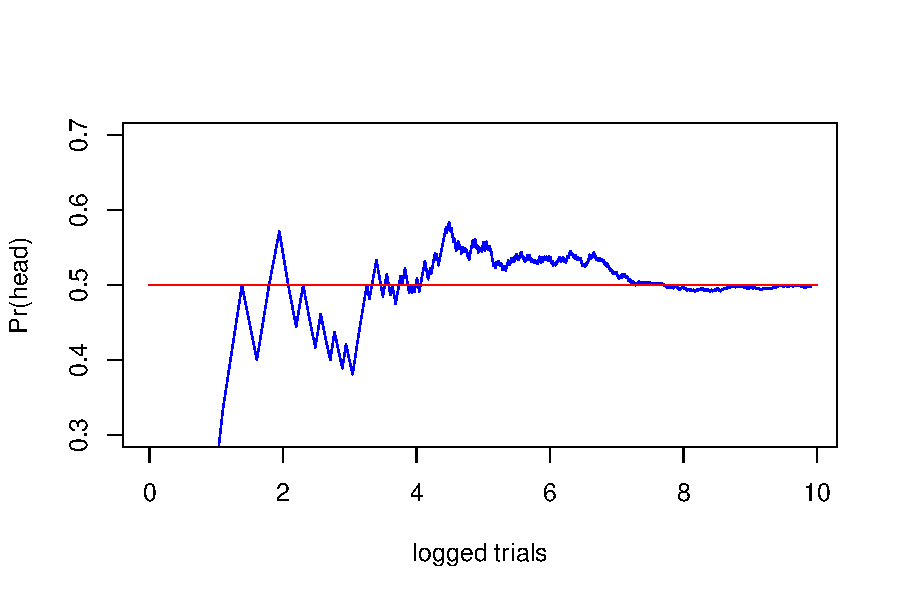
\includegraphics{Econometrics2TA_files/figure-latex/WLLN-1.pdf}
\caption{\label{fig:WLLN}Simulation Result of WLLN}
\end{figure}

\hypertarget{central-limit-theorem}{%
\paragraph{Central Limit Theorem}\label{central-limit-theorem}}

The second important theorm is the \textbf{central limit theorem}.
Suppose that \(X_i, \ldots, X_n\) are IID sample with mean \(\mu\) and variance \(\sigma^2\).
This theorem says that the sample mean \(\bar{X}_n\) has a distribution
which is approximately normal with mean \(\mu\) and variance \(\sigma^2/n\).
This theorem does not assume the distribution of \(X_i\), except the existence of the mean and variance.
Formally,

\begin{quote}
Let \(X_1, \ldots, X_n\) be IID with mean \(\mu\) and variance \(\sigma^2\).
Let \(\bar{X}_n = n^{-1} \sum_{i=1}^n X_i\). Then,
\begin{align*}
Z_n \equiv \frac{\bar{X}_n - \mu}{\sqrt{V(\bar{X}_n)}} = \sqrt{n}\frac{\bar{X}_n - \mu}{\sigma} \stackrel{d}{\to} Z,
\end{align*}
where \(Z \sim N(0, 1)\). In other words, \(\bar{X}_n \stackrel{d}{\to} N(\mu, \sigma^2/n)\).
\end{quote}

As an illustlation, consider a fair coin toss.
The random variable is the number of heads.
This random variable has the Bernoulli distribution with mean \(\mu = 0.5\) and variance \(\sigma^2 = 0.5(1 - 0.5) = 0.25\).
Since we know \(\mu\) and \(\sigma^2\), we can calculate \(Z_n\), using the sample mean \(\bar{X}_n\).
We work this and plot its distribution, using R programming.
We generate 10,000 sample means \(\bar{X}_n\) for \(n = 3, 5, 100, 1000\), and transform sample means to \(Z_n\).
To calculate \(Z_n\), we use command \texttt{sqrt()}, which returns the saquare root value.
Sometimes, this procedure is called Monte-Carlo simulation.

\begin{Shaded}
\begin{Highlighting}[]
\KeywordTok{set.seed}\NormalTok{(}\DecValTok{120504}\NormalTok{)}
\NormalTok{m \textless{}{-}}\StringTok{ }\DecValTok{10000}\NormalTok{; n \textless{}{-}}\StringTok{ }\KeywordTok{c}\NormalTok{(}\DecValTok{3}\NormalTok{, }\DecValTok{100}\NormalTok{, }\DecValTok{1000}\NormalTok{); p \textless{}{-}}\StringTok{ }\FloatTok{0.5}
\NormalTok{a \textless{}{-}}\StringTok{ }\KeywordTok{seq}\NormalTok{(}\OperatorTok{{-}}\DecValTok{4}\NormalTok{, }\DecValTok{4}\NormalTok{, }\FloatTok{.01}\NormalTok{); b \textless{}{-}}\StringTok{ }\KeywordTok{dnorm}\NormalTok{(a)}

\NormalTok{dt \textless{}{-}}\StringTok{ }\KeywordTok{list}\NormalTok{(}\StringTok{"n = 3"}\NormalTok{=}\KeywordTok{numeric}\NormalTok{(m), }\StringTok{"n = 100"}\NormalTok{=}\KeywordTok{numeric}\NormalTok{(m), }\StringTok{"n = 1000"}\NormalTok{=}\KeywordTok{numeric}\NormalTok{(m))}
\ControlFlowTok{for}\NormalTok{ (i }\ControlFlowTok{in} \DecValTok{1}\OperatorTok{:}\DecValTok{3}\NormalTok{) \{}
\NormalTok{  dt[[i]] \textless{}{-}}\StringTok{ }\KeywordTok{rbinom}\NormalTok{(}\DataTypeTok{n =}\NormalTok{ m, }\DataTypeTok{size =}\NormalTok{ n[i], }\DataTypeTok{prob =}\NormalTok{ p)}
\NormalTok{  dt[[i]] \textless{}{-}}\StringTok{ }\KeywordTok{sqrt}\NormalTok{(n[i])}\OperatorTok{*}\NormalTok{(dt[[i]]}\OperatorTok{/}\NormalTok{n[i] }\OperatorTok{{-}}\StringTok{ }\NormalTok{p)}\OperatorTok{/}\KeywordTok{sqrt}\NormalTok{(p}\OperatorTok{*}\NormalTok{(}\DecValTok{1}\OperatorTok{{-}}\NormalTok{p))}
\NormalTok{\}}

\KeywordTok{par}\NormalTok{(}\DataTypeTok{mfrow=}\KeywordTok{c}\NormalTok{(}\DecValTok{2}\NormalTok{,}\DecValTok{2}\NormalTok{), }\DataTypeTok{mai =} \KeywordTok{c}\NormalTok{(}\FloatTok{0.5}\NormalTok{, }\FloatTok{0.5}\NormalTok{, }\FloatTok{0.35}\NormalTok{, }\FloatTok{0.35}\NormalTok{)) }
\ControlFlowTok{for}\NormalTok{ (i }\ControlFlowTok{in} \DecValTok{1}\OperatorTok{:}\DecValTok{3}\NormalTok{) \{}
  \KeywordTok{hist}\NormalTok{(dt[[i]], }\DataTypeTok{col =} \StringTok{"grey"}\NormalTok{, }\DataTypeTok{freq =} \OtherTok{FALSE}\NormalTok{, }
    \DataTypeTok{xlab =} \StringTok{""}\NormalTok{, }\DataTypeTok{main =} \KeywordTok{names}\NormalTok{(dt)[i], }\DataTypeTok{xlim =} \KeywordTok{c}\NormalTok{(}\OperatorTok{{-}}\DecValTok{4}\NormalTok{, }\DecValTok{4}\NormalTok{))}
  \KeywordTok{par}\NormalTok{(}\DataTypeTok{new =} \OtherTok{TRUE}\NormalTok{)}
  \KeywordTok{plot}\NormalTok{(a, b, }\DataTypeTok{type =} \StringTok{"l"}\NormalTok{, }\DataTypeTok{col =} \StringTok{"red"}\NormalTok{, }\DataTypeTok{axes =} \OtherTok{FALSE}\NormalTok{, }
    \DataTypeTok{xlab =} \StringTok{""}\NormalTok{, }\DataTypeTok{ylab =} \StringTok{""}\NormalTok{, }\DataTypeTok{main =} \StringTok{""}\NormalTok{)}
\NormalTok{\}}
\end{Highlighting}
\end{Shaded}

\begin{figure}
\centering
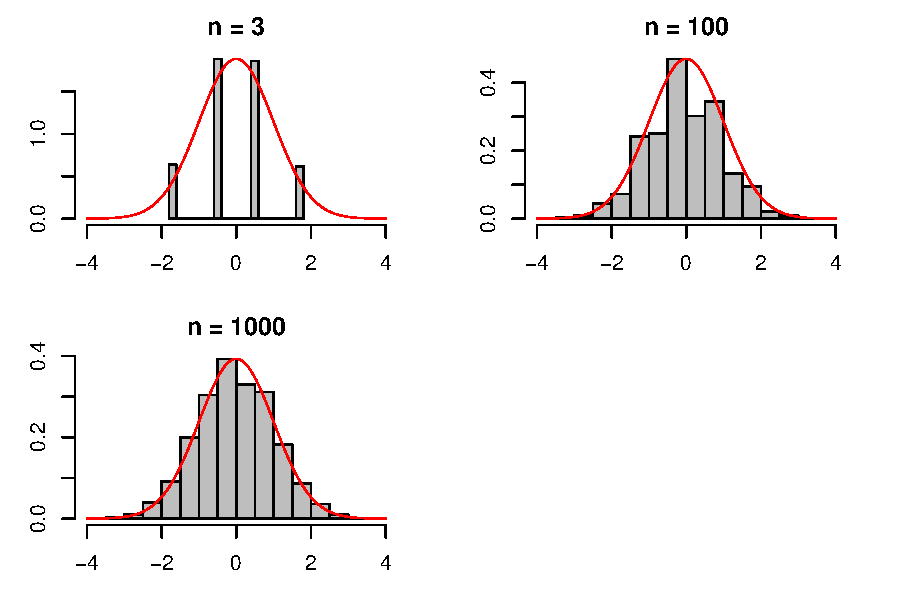
\includegraphics{Econometrics2TA_files/figure-latex/CLT-1.pdf}
\caption{\label{fig:CLT}Simulation Result of CLT}
\end{figure}

\hypertarget{reviews-of-ordinary-least-squares-and-maximum-likelihood-estimation}{%
\section{Reviews of Ordinary Least Squares and Maximum Likelihood Estimation}\label{reviews-of-ordinary-least-squares-and-maximum-likelihood-estimation}}

This section refers to Johnston (1984) and Angrist and Pischke (2008).
Consider the \(k\)-variables lienar regression model:
\begin{align*}
  y_i = x_i \beta + u_i,
\end{align*}
where \(\beta = (\beta_0, \beta_1, \ldots, \beta_k)'\) is a \(k \times 1\) vector of regression coefficients,
\(x_i = (1, x_{i1}, \ldots, x_{ik})\) is a \(1 \times k\) vector of stochastic covariates,
and \(u_i\) is the error term which is idependent and identically distributed (i.i.d.).
Our parameter of interest is \(\beta\).

\hypertarget{ordinary-least-squares-estimator-olse}{%
\subsection{Ordinary Least Squares Estimator (OLSE)}\label{ordinary-least-squares-estimator-olse}}

The \textbf{OLS estimators} are the value \(\beta\) such that minimizing the residual sums of squares,
that is,

\begin{quote}
The \textbf{OLS estimators} \(\hat{\beta}\) is defined by
\begin{align*}
\hat{\beta} \in \mathop{\rm arg~min}\limits_{\beta} \sum_{i = 1}^n (y_i - x_i \beta)^2,
\end{align*}
or,
\begin{align*}
\hat{\beta} \in \mathop{\rm arg~min}\limits_{\beta} (Y - X \beta)'(Y - X \beta),
\end{align*}
where \(Y = (y_1, \ldots, y_n)'\) is a \(n \times 1\) vector, and
\(X = (x_1, \ldots, x_n)'\) is a \(n \times k\).
\end{quote}

Following this definition, the OLSE is given by
\begin{align*}
  \hat{\beta} = (X'X)^{-1}(X'Y).
\end{align*}
To exist the inverse matrix, we assume that the matrix \((X'X)\) is the regular matrix
(i.e., there is no perfect correlation between any two covariates).

\hypertarget{best-linear-unbiased-estimator-blue}{%
\subsubsection{Best Linear Unbiased Estimator (BLUE)}\label{best-linear-unbiased-estimator-blue}}

We impose assumptions about the disturbance vector \(u\):
(i) \(E(u|X) = 0\) (exogenity assumption or mean-idependence),
and (ii) \(V(u|X) = \sigma^2 I\) (homoscedasticity and pairwise uncorrelation).
Under this condition, the OLS estimator is a linear unbiased estimator, that is, \(E(\hat{\beta}) = \beta\) since
\begin{align*}
  E(\hat{\beta}|X) = E[\beta + (X'X)^{-1}(X'u)|X] = \beta + (X'X)^{-1}X'E(u|X) = \beta.
\end{align*}
Furthermore, the variance-covariance matrix of OLSE is
\begin{align*}
  V(\hat{\beta}|X) 
  &= E[(X'X)^{-1}X' uu' X (X'X)^{-1} | X] \\
  &= (X'X)^{-1}X' \sigma^2 I X (X'X)^{-1} \\
  &= \sigma^2 (X'X)^{-1}.
\end{align*}
Note that \(V(\hat{\beta}) = \sigma^2 E[ (X'X)^{-1} ]\).
The most important result is that
no other linear unbiased estimator can have smaller variances than those of OLSE.
In other words, the OLSE has minimum variance within the class of linear unbiased estimators.
Thus, the OLSE is a best linear unbiased estimator (\textbf{BLUE}).
This result is known as the \emph{Gauss-Markov theorem} (We omit proof).

\hypertarget{asymptotic-properties}{%
\subsubsection{Asymptotic Properties}\label{asymptotic-properties}}

First, the OLSE is a consistent estimator, that is,
\begin{align*}
  \mathop{\mathrm{plim}}\hat{\beta} = \beta + \mathop{\mathrm{plim}}\left( \frac{1}{n} (X'X) \right)^{-1} \mathop{\mathrm{plim}}\left( \frac{1}{n} X'u \right) = \beta.
\end{align*}
This is bacause \(\mathop{\mathrm{plim}}n^{-1} (X'X) = \mathop{\mathrm{plim}}n^{-1} \sum_i x'_i x_i = E[x'_i x_i] = \Sigma\)
and \(\mathop{\mathrm{plim}}n^{-1} (X'u) = \mathop{\mathrm{plim}}n^{-1} \sum_i x'_i u_i = E[x'_i u_i] = 0\)
by mean-independence assumption.

Second, the OLSE is asymptotically normally distributed.
To show it, we derive the asymptotic distribution of \(\sqrt{n}(\hat{\beta} - \beta)\) where
\begin{align*}
  \sqrt{n}(\hat{\beta} - \beta) = \left( \frac{1}{n} \sum_i x'_i x_i \right)^{-1} \sqrt{n} \left( \frac{1}{n} \sum_i x'_i u_i \right).
\end{align*}
By the central theorem, we have
\begin{align*}
  \sqrt{n} \left( \frac{1}{n} \sum_i x'_i u_i \right) \overset{d}{\to} N(0, \sigma^2 \Sigma).
\end{align*}
Recall that \(n^{-1} \sum_i x'_i x_i \overset{p}{\to} \Sigma\).
By the Slutsky theorem (the 6th property of convergence), we get
\begin{align*}
  \sqrt{n}(\hat{\beta} - \beta) \overset{d}{\to} N(0, \sigma^2 \Sigma^{-1}),
\end{align*}
or,
\begin{align*}
  \hat{\beta} \overset{d}{\to} N \left(\beta, \frac{1}{n} \sigma^2 \Sigma^{-1} \right).
\end{align*}

In a practical application, the unknown \(\Sigma\) is replaced by the sample estimate \(n^{-1} X'X\),
and the unknown \(\sigma^2\) is estimated by \(\hat{\sigma}^2 = \hat{u}'\hat{u}/(n-k)\)
where \(\hat{u} = Y - X \hat{\beta} = (I_n - X(X'X)^{-1}X')u = M_X u\) and \(M_X\) is a symmetric and idempotent matrix.
Note that \(\hat{\sigma}^2\) is an unbiased estimator of \(\sigma^2\) since
\begin{align*}
  E[ \hat{\sigma}^2 ] = \frac{1}{n-k} E[tr(M_X uu')] = \frac{\sigma^2}{n-k} tr(M_X I_n) = \sigma^2. 
\end{align*}

\hypertarget{finite-sample-distribution-and-inference}{%
\subsubsection{Finite-sample Distribution and Inference}\label{finite-sample-distribution-and-inference}}

Now, we add the assumption with respect to the error term, \(\epsilon_i |x_i \overset{iid}{\sim} N(0, \sigma^2)\).
Then, we immediately obtain
\begin{align*}
  \hat{\beta}|X \sim N(\beta, \sigma^2(X'X)^{-1}).
\end{align*}

Consider the set of linear null hypothesis embodied in \(R \beta = r\)
where \(R\) is a arbitrary \(q \times k\) matrix and \(r\) is a known \(q\)-element vector.
To develop a test procedure, we derive the exact distribution of \(R\hat{\beta}\).
Cleary, we see \(E(R\hat{\beta}) = R\beta\) and \(V(R\hat{\beta}) = \sigma^2 R (X'X)^{-1} R'\).
This leads to
\begin{align*}
  R(\hat{\beta} - \beta) \sim N(0, \sigma^2 R (X'X)^{-1} R').
\end{align*}
If the null hypothesis is true, then
\begin{align*}
  R\hat{\beta} - r \sim N(0, \sigma^2 R (X'X)^{-1} R').
\end{align*}
Using it and \(\hat{u}'\hat{u} = u' M_X u\), we have follwing two distributions
\begin{align*}
  &(R\hat{\beta} - r)'[\sigma^2 R (X'X)^{-1} R']^{-1}(R\hat{\beta} - r) \sim \chi^2(q),  \\
  &\frac{\hat{u}'\hat{u}}{\sigma^2} \sim \chi^2(n - k)
\end{align*}
To derive these distributions, we use the following two properties about chi-squared distribution:

\begin{itemize}
\tightlist
\item
  If \(x \sim N(0, \Sigma)\), then \(x'\Sigma x \sim \chi^2(n)\) where \(x\) is \(n\)-element vector.
\item
  If \(x \sim N(0, \sigma^2 I)\) and \(A\) is idempotent matrix, then \((\sigma^2)^{-1} x'Ax \sim \chi^2(tr(A))\).
\end{itemize}

Finally, since \(X_1 \sim \chi^2(d_1)\) and \(X_2 \sim \chi^2(d_2)\) lead to \(\frac{X_1}{d_1}/\frac{X_2}{d_2} \sim F(d_1, d_2)\),
we have the distribution of test statistic, called the F-distribution,
\begin{align*}
  \frac{(R\hat{\beta} - r)'[R (X'X)^{-1} R']^{-1}(R\hat{\beta} - r)/q}{\hat{u}'\hat{u}/(n - k)} \sim F(q, n-k).
\end{align*}
The test procedure is to reject the null hypothesis \(R\beta = r\) if the computed F-value exceeds a preselected cricial value.

Especially, when we test a single coefficient, we can use the t-value as an alternative test statistic.
Suppose that \(R = (0, 1, 0, \ldots, 0)\) and \(r = 0\).
The null hypothesis is \(\hat{\beta}_2 = 0\).
The matrix \(R (X'X)^{-1} R'\) picks up the second diagonal element of \((X'X)^{-1}\) denoted by \((X'X)^{-1}_{22}\).
Then, we have
\begin{align*}
  \frac{\hat{\beta}_2^2}{\hat{\sigma}^2 (X'X)^{-1}_{22}} \sim F(1, n-k).
\end{align*}
Since \(t \sim t(n)\) is equivalent to \(t^2 \sim F(1, n)\) for any \(n\),
we finally obtain the test statistic following the Student's t-distribution
\begin{align*}
  \frac{\hat{\beta}_2}{\hat{\sigma} \sqrt{(X'X)^{-1}_{22}}} \sim t(n - k).
\end{align*}
When you use t-test of a single coefficient, you should \emph{two-sided} t-test.
If the computed t-statistic \(\hat{t}\) holds \(|\hat{t}| > t_{1-\alpha/2}(n-k)\)
where \(t_{q}(n-k)\) is the \(q\)-percentile t-value,
then we can reject the null hyporhesis \(\hat{\beta}_2 = 0\)

\hypertarget{maximum-likelihood-estimator-mle}{%
\subsection{Maximum Likelihood Estimator (MLE)}\label{maximum-likelihood-estimator-mle}}

When we assume that the error term is normally distributed, we have \(y_i | x_i \overset{iid}{\sim} N(x_i \beta, \sigma^2)\).
Under this assumption, the estimator \(\tilde{\beta}\) maximizing the log-likelihood function, called \textbf{maximum likelihood estimator},
is equivalent to the OLSE.
The likelihood function is
\begin{align*}
  \prod_{i=1}^n f(y_i, x_i)
  = \prod_{i=1}^n f_{Y|X}(y_i | x_i) \prod_{i=1}^n f_X(x_i)
  = \sum_{i=1}^n \log f_{Y|X}(y_i | x_i) + \sum_{i=1}^n \log f_X(x_i).
\end{align*}
Since \(f_X(x_i)\) does not involve the parameter vector \(\beta\),
the \emph{conditional} MLE \(\tilde{\beta}\) maximizes the conditional log-likelihood function \(\sum_{i=1}^n \log f_i(y_i | x_i)\), that is,
\begin{align*}
  \log L(\theta) 
  &= \sum_{i=1}^n \log f_{Y|X}(y_i | x_i)  \\
  &= \sum_{i=1}^n \log \left( (2\pi\sigma^2)^{-1/2} \exp\left( -\frac{(y_i - x_i \beta)^2}{2\sigma^2} \right) \right)  \\
  &= -\frac{n}{2} \log (2\pi) -\frac{n}{2}\log\sigma^2 -\frac{1}{2\sigma^2} (Y - X \beta)'(Y - X \beta),
\end{align*}
where \(\theta = (\beta', \sigma^2)'\) is a \((k + 1) \times 1\) vector of unknown parameters.
The first-order derivatives of this function, sometimes called \textbf{score}, is given by
\begin{align*}
  \frac{\partial \log L(\theta)}{\partial \theta} =
  \begin{pmatrix}
    -\frac{1}{2\sigma^2} (-2X'Y + 2X'X \beta) \\
    -\frac{1}{2\sigma^2} \left(n - \frac{1}{\sigma^2} (Y - X \beta)'(Y - X \beta) \right)
  \end{pmatrix}.
\end{align*}
The necessary condition of MLE is \(\frac{\partial}{\partial \theta} \log L(\theta) = 0\).
This leads to the following MLE:
\begin{align*}
  \tilde{\beta} = (X'X)^{-1}(X'Y),\quad \tilde{\sigma}^2 = \frac{\hat{u}'\hat{u}}{n}.
\end{align*}
The sufficient condition of MLE is the following Hessian matrix is negative definite.
\begin{align*}
  H(\theta) =
  \begin{pmatrix}
    -\frac{1}{\sigma^2} X'X  & \frac{1}{2\sigma^4} (-X'Y + X'X \beta) \\
    \frac{1}{2\sigma^4} (-X'Y + X'X \beta) & \frac{n}{2\sigma^4} - \frac{1}{\sigma^6} (Y - X \beta)'(Y - X \beta)
  \end{pmatrix}.
\end{align*}

\hypertarget{properties-of-mle}{%
\subsection{Properties of MLE}\label{properties-of-mle}}

First, we provide the \emph{Cramer-Rao theorem} that states that ML methods gives the lower bound of variance of unbiased estimators
(proof is omitted).

\begin{quote}
Let \(\tilde{\theta}\) denote an unbiased estimator of \(\theta\). Then, \(V(\tilde{\theta}) - I^{-1}(\theta)\) is a positive definite where
\(I(\theta)\) is a \textbf{Fisher information matrix}, which is defined by
\begin{align*}
I(\theta) 
= - E (H(\theta)) 
= - E 
\begin{pmatrix}
\frac{\partial^2 \log L(\theta) }{\partial \theta_1^2} &
\frac{\partial^2 \log L(\theta) }{\partial \theta_1 \partial \theta_2} &
\cdots &
\frac{\partial^2 \log L(\theta) }{\partial \theta_1 \partial \theta_k} \\
\frac{\partial^2 \log L(\theta) }{\partial \theta_2 \partial \theta_1} &
\frac{\partial^2 \log L(\theta) }{\partial \theta_2^2} &
\cdots &
\frac{\partial^2 \log L(\theta) }{\partial \theta_2 \partial \theta_k} \\
\vdots & \vdots & \vdots & \vdots \\
\frac{\partial^2 \log L(\theta) }{\partial \theta_k \partial \theta_1} &
\frac{\partial^2 \log L(\theta) }{\partial \theta_k \partial \theta_2} &
\cdots &
\frac{\partial^2 \log L(\theta) }{\partial \theta_k^2}
\end{pmatrix}.
\end{align*}
\end{quote}

Note that the Fisher information matrix conditional on some random variables
also provides the Cramer-Rao lower bound.
In the case of linear regression, the Cramer-Rao lower bound condtional on \(X\) gives
\begin{align*}
  I^{-1} \begin{pmatrix} \beta \\ \sigma^2 \end{pmatrix}
  = 
  \begin{pmatrix} \sigma^2 X'X^{-1} & 0 \\ 0 & \frac{2\sigma^4}{n} \end{pmatrix}.
\end{align*}
Although the ML estimator of \(\beta\) attains the Cramer-Rao lower bound,
the ML estimator of \(\sigma^2\) deviates.

Second, we summarize asymptotic properties of MLE as follows (proof is omitted):

\begin{quote}
Under certain regularity conditions,
(i) The ML estimator is consistent, i.e., \(\tilde{\theta} \overset{p}{\to} \theta\), and
(ii) The ML estimator is asymptotically normally distributed, i.e., \(\tilde{\theta} \overset{d}{\to} N(\theta, I^{-1}(\theta))\)
\end{quote}

\hypertarget{qualitative-models}{%
\section{Qualitative Models}\label{qualitative-models}}

\hypertarget{empirical-application-of-binary-model-titanic-survivors}{%
\subsection{Empirical Application of Binary Model: Titanic Survivors}\label{empirical-application-of-binary-model-titanic-survivors}}

\hypertarget{background-and-data}{%
\subsubsection{Background and Data}\label{background-and-data}}

``Women and children first'' is a behavioral norm,
which women and children are saved first in a life-threatening situation.
This code was made famous by the sinking of the Titanic in 1912.
An empirical application investigates characteristics of survivors of Titanic
to answer whether crews obeyed the code or not.

We use an open data about Titanic survivors.\footnote{data source: \url{http://biostat.mc.vanderbilt.edu/DataSets}.}
Number of observations is 1,045.
Although this dataset contains many variables,
we use only four variables: \texttt{survived}, \texttt{age}, \texttt{fare}, and \texttt{sex}.
We summarize descriptions of variables as follows:

\begin{itemize}
\tightlist
\item
  \texttt{survived}: a binary variable taking 1 if a passenger survived.
\item
  \texttt{age}: a continuous variable representing passeger's age.
\item
  \texttt{fare}: a continuous variable representing how much passeger paid.
\item
  \texttt{sex}: a string variable representing passenger's sex.
\end{itemize}

Using \texttt{sex}, we will make a binary variable, called \texttt{female}, taking 1 if passeger is female.
Intead of \texttt{sex}, we use \texttt{female} variable in regression.

Moreover, we split data into two subsets: the \emph{training} data and the \emph{test} data.
The training data is randomly drawn from the original data.
The sample size of this data is two thirs of total observations, that is, \(N = 696\).
We use the training data (\emph{in-sample}) to estimate and evaluate model fitness.
The test data consists of observations which the training data does not include (\(N = 349\)).
We use the test data (\emph{out-of-sample}) to evaluate model prediction.

\begin{Shaded}
\begin{Highlighting}[]
\NormalTok{dt \textless{}{-}}\StringTok{ }\KeywordTok{read.csv}\NormalTok{(}
  \DataTypeTok{file =} \StringTok{"./data/titanic.csv"}\NormalTok{, }
  \DataTypeTok{header =} \OtherTok{TRUE}\NormalTok{,  }\DataTypeTok{sep =} \StringTok{","}\NormalTok{, }\DataTypeTok{row.names =} \OtherTok{NULL}\NormalTok{,  }\DataTypeTok{stringsAsFactors =} \OtherTok{FALSE}\NormalTok{)}

\NormalTok{dt}\OperatorTok{$}\NormalTok{female \textless{}{-}}\StringTok{ }\KeywordTok{ifelse}\NormalTok{(dt}\OperatorTok{$}\NormalTok{sex }\OperatorTok{==}\StringTok{ "female"}\NormalTok{, }\DecValTok{1}\NormalTok{, }\DecValTok{0}\NormalTok{)}
\NormalTok{dt \textless{}{-}}\StringTok{ }\KeywordTok{subset}\NormalTok{(dt, }\OperatorTok{!}\KeywordTok{is.na}\NormalTok{(survived)}\OperatorTok{\&!}\KeywordTok{is.na}\NormalTok{(age)}\OperatorTok{\&!}\KeywordTok{is.na}\NormalTok{(fare)}\OperatorTok{\&!}\KeywordTok{is.na}\NormalTok{(female))}
\NormalTok{dt \textless{}{-}}\StringTok{ }\NormalTok{dt[,}\KeywordTok{c}\NormalTok{(}\StringTok{"survived"}\NormalTok{, }\StringTok{"age"}\NormalTok{, }\StringTok{"fare"}\NormalTok{, }\StringTok{"female"}\NormalTok{)]}

\KeywordTok{set.seed}\NormalTok{(}\DecValTok{120511}\NormalTok{)}
\NormalTok{train\_id \textless{}{-}}\StringTok{ }\KeywordTok{sample}\NormalTok{(}\DecValTok{1}\OperatorTok{:}\KeywordTok{nrow}\NormalTok{(dt), }\DataTypeTok{size =}\NormalTok{ (}\DecValTok{2}\OperatorTok{/}\DecValTok{3}\NormalTok{)}\OperatorTok{*}\KeywordTok{nrow}\NormalTok{(dt), }\DataTypeTok{replace =} \OtherTok{FALSE}\NormalTok{)}
\NormalTok{train\_dt \textless{}{-}}\StringTok{ }\NormalTok{dt[train\_id,]}
\NormalTok{test\_dt \textless{}{-}}\StringTok{ }\NormalTok{dt[}\OperatorTok{{-}}\NormalTok{train\_id,]}

\KeywordTok{head}\NormalTok{(dt)}
\end{Highlighting}
\end{Shaded}

\begin{verbatim}
##   survived   age     fare female
## 1        1 29.00 211.3375      1
## 2        1  0.92 151.5500      0
## 3        0  2.00 151.5500      1
## 4        0 30.00 151.5500      0
## 5        0 25.00 151.5500      1
## 6        1 48.00  26.5500      0
\end{verbatim}

\noindent
\textbf{Model}.
In a binary model, a dependent (outcome) variable \(y_i\) takes only two values, i.e., \(y_i \in \{0, 1\}\).
A binary variable is sometimes called a \emph{dummy} variable.
In this application, the outcome variable is \texttt{survived}.
Explanatory variables are \texttt{female}, \texttt{age}, and \texttt{fare}.
The regression function is
\begin{equation*}
  \begin{split}
    &E[survived | female, age, fare] \\
    =& \mathbb{P}[survived = 1 | female, age, fare]
    = G(\beta_0 + \beta_1 female + \beta_2 age + \beta_3 fare).
  \end{split}
\end{equation*}
The function \(G(\cdot)\) is arbitrary function. In practice, we often use following three specifications:

\begin{itemize}
\tightlist
\item
  Linear probability model (LPM): \(G(\mathbf{x}_i \beta) = \mathbf{x}_i \beta\).
\item
  Probit model: \(G(\mathbf{x}_i \beta) = \Phi(\mathbf{x}_i \beta)\) where \(\Phi(\cdot)\) is the standard Gaussian cumulative function.
\item
  Logit model: \(G(\mathbf{x}_i \beta) = 1/(1 + \exp(-\mathbf{x}_i \beta))\).
\end{itemize}

\hypertarget{linear-probability-model}{%
\subsubsection{Linear Probability Model}\label{linear-probability-model}}

The linear probability model specifys that \(G(a)\) is linear in \(a\), that is,
\begin{equation*}
  \mathbb{P}[survived = 1 | female, age, fare]
  = \beta_0 + \beta_1 female + \beta_2 age + \beta_3 fare.
\end{equation*}
This model can be estimated using the OLS method.
In \texttt{R}, we can use the OLS method, running \texttt{lm()} function.

\begin{Shaded}
\begin{Highlighting}[]
\NormalTok{model \textless{}{-}}\StringTok{ }\NormalTok{survived }\OperatorTok{\textasciitilde{}}\StringTok{ }\KeywordTok{factor}\NormalTok{(female) }\OperatorTok{+}\StringTok{ }\NormalTok{age }\OperatorTok{+}\StringTok{ }\NormalTok{fare}
\NormalTok{LPM \textless{}{-}}\StringTok{ }\KeywordTok{lm}\NormalTok{(model, }\DataTypeTok{data =}\NormalTok{ train\_dt)}
\end{Highlighting}
\end{Shaded}

The linear probability model is heteroskedastic,
that is, \(V(u_i | \mathbf{x}_i) = G(\mathbf{x}_i \beta)(1 - G(\mathbf{x}_i \beta))\).
However, \texttt{lm()} function assumes homoskedasticity.
To resolve it, we need to claculate heteroskedasticity-robust standard errors using the White method.
\begin{equation*}
  \hat{V}(\hat{\beta}) =
  \left( \frac{1}{n} \sum_i \mathbf{x}'_i \mathbf{x}_i  \right)^{-1}
  \left( \frac{1}{n} \sum_i \hat{u}_i^2 \mathbf{x}'_i \mathbf{x}_i \right)
  \left( \frac{1}{n} \sum_i \mathbf{x}'_i \mathbf{x}_i \right)^{-1}
\end{equation*}
where \(\hat{u}_i = y_i - G(\mathbf{x}_i \hat{\beta})\).

\begin{Shaded}
\begin{Highlighting}[]
\CommentTok{\# heteroskedasticity{-}robust standard errors}
\NormalTok{train\_dt}\OperatorTok{$}\StringTok{"(Intercept)"}\NormalTok{ \textless{}{-}}\StringTok{ }\DecValTok{1}
\NormalTok{X \textless{}{-}}\StringTok{ }\KeywordTok{as.matrix}\NormalTok{(train\_dt[,}\KeywordTok{c}\NormalTok{(}\StringTok{"(Intercept)"}\NormalTok{, }\StringTok{"female"}\NormalTok{, }\StringTok{"age"}\NormalTok{, }\StringTok{"fare"}\NormalTok{)])}
\NormalTok{u \textless{}{-}}\StringTok{ }\KeywordTok{diag}\NormalTok{(LPM}\OperatorTok{$}\NormalTok{residuals}\OperatorTok{\^{}}\DecValTok{2}\NormalTok{)}

\NormalTok{XX \textless{}{-}}\StringTok{ }\KeywordTok{t}\NormalTok{(X) }\OperatorTok{\%*\%}\StringTok{ }\NormalTok{X}
\NormalTok{avgXX \textless{}{-}}\StringTok{ }\NormalTok{XX }\OperatorTok{*}\StringTok{ }\KeywordTok{nrow}\NormalTok{(X)}\OperatorTok{\^{}}\NormalTok{\{}\OperatorTok{{-}}\DecValTok{1}\NormalTok{\}}
\NormalTok{inv\_avgXX \textless{}{-}}\StringTok{ }\KeywordTok{solve}\NormalTok{(avgXX)}

\NormalTok{uXX \textless{}{-}}\StringTok{ }\KeywordTok{t}\NormalTok{(X) }\OperatorTok{\%*\%}\StringTok{ }\NormalTok{u }\OperatorTok{\%*\%}\StringTok{ }\NormalTok{X}
\NormalTok{avguXX \textless{}{-}}\StringTok{ }\NormalTok{uXX }\OperatorTok{*}\StringTok{ }\KeywordTok{nrow}\NormalTok{(X)}\OperatorTok{\^{}}\NormalTok{\{}\OperatorTok{{-}}\DecValTok{1}\NormalTok{\} }

\NormalTok{vcov\_b \textless{}{-}}\StringTok{ }\NormalTok{(inv\_avgXX }\OperatorTok{\%*\%}\StringTok{ }\NormalTok{avguXX }\OperatorTok{\%*\%}\StringTok{ }\NormalTok{inv\_avgXX) }\OperatorTok{*}\StringTok{ }\KeywordTok{nrow}\NormalTok{(X)}\OperatorTok{\^{}}\NormalTok{\{}\OperatorTok{{-}}\DecValTok{1}\NormalTok{\}}
\NormalTok{rse\_b \textless{}{-}}\StringTok{ }\KeywordTok{sqrt}\NormalTok{(}\KeywordTok{diag}\NormalTok{(vcov\_b))}

\NormalTok{label \textless{}{-}}\StringTok{ }\KeywordTok{c}\NormalTok{(}\StringTok{"(Intercept)"}\NormalTok{, }\StringTok{"factor(female)1"}\NormalTok{, }\StringTok{"age"}\NormalTok{, }\StringTok{"fare"}\NormalTok{)}
\KeywordTok{names}\NormalTok{(rse\_b) \textless{}{-}}\StringTok{ }\NormalTok{label}

\CommentTok{\# homoskedasticity{-}based standard errors}
\NormalTok{se\_b \textless{}{-}}\StringTok{ }\KeywordTok{sqrt}\NormalTok{(}\KeywordTok{diag}\NormalTok{(}\KeywordTok{vcov}\NormalTok{(LPM)))}

\KeywordTok{print}\NormalTok{(}\StringTok{"The Variance of OLS"}\NormalTok{); }\KeywordTok{vcov}\NormalTok{(LPM)}
\end{Highlighting}
\end{Shaded}

\begin{verbatim}
## [1] "The Variance of OLS"
\end{verbatim}

\begin{verbatim}
##                   (Intercept) factor(female)1           age          fare
## (Intercept)      1.505787e-03   -3.905773e-04 -3.676396e-05 -5.951346e-07
## factor(female)1 -3.905773e-04    1.089299e-03  2.569835e-06 -2.154400e-06
## age             -3.676396e-05    2.569835e-06  1.264948e-06 -6.274261e-08
## fare            -5.951346e-07   -2.154400e-06 -6.274261e-08  9.167801e-08
\end{verbatim}

\begin{Shaded}
\begin{Highlighting}[]
\KeywordTok{print}\NormalTok{(}\StringTok{"The Robust variance of OLS"}\NormalTok{); vcov\_b}
\end{Highlighting}
\end{Shaded}

\begin{verbatim}
## [1] "The Robust variance of OLS"
\end{verbatim}

\begin{verbatim}
##               (Intercept)        female           age          fare
## (Intercept)  1.810499e-03 -3.968956e-04 -4.601203e-05  8.979498e-07
## female      -3.968956e-04  1.239665e-03  4.975911e-06 -4.566026e-06
## age         -4.601203e-05  4.975911e-06  1.476806e-06 -7.956793e-08
## fare         8.979498e-07 -4.566026e-06 -7.956793e-08  7.846876e-08
\end{verbatim}

\begin{Shaded}
\begin{Highlighting}[]
\KeywordTok{print}\NormalTok{(}\StringTok{"The Robust se using White method"}\NormalTok{); rse\_b}
\end{Highlighting}
\end{Shaded}

\begin{verbatim}
## [1] "The Robust se using White method"
\end{verbatim}

\begin{verbatim}
##     (Intercept) factor(female)1             age            fare 
##    0.0425499596    0.0352088828    0.0012152389    0.0002801228
\end{verbatim}

Using the package \texttt{lmtest} and \texttt{sandwich} is
the easiest way to calculate heteroskedasticity-robust standard errors.

\begin{Shaded}
\begin{Highlighting}[]
\KeywordTok{library}\NormalTok{(lmtest) }\CommentTok{\#use function \textasciigrave{}coeftest\textasciigrave{}}
\KeywordTok{library}\NormalTok{(sandwich) }\CommentTok{\#use function \textasciigrave{}vcovHC\textasciigrave{}}
\KeywordTok{coeftest}\NormalTok{(LPM, }\DataTypeTok{vcov =} \KeywordTok{vcovHC}\NormalTok{(LPM, }\DataTypeTok{type =} \StringTok{"HC0"}\NormalTok{))[, }\StringTok{"Std. Error"}\NormalTok{]}
\end{Highlighting}
\end{Shaded}

\begin{verbatim}
##     (Intercept) factor(female)1             age            fare 
##    0.0425499596    0.0352088828    0.0012152389    0.0002801228
\end{verbatim}

Finally, we summarize results of linear probability model in table \ref{LPM}.
We will discuss interpretation of results and goodness-of-fit of LPM later.

\begin{Shaded}
\begin{Highlighting}[]
\KeywordTok{library}\NormalTok{(stargazer)}
\KeywordTok{stargazer}\NormalTok{(}
\NormalTok{  LPM, LPM,}
  \DataTypeTok{se =} \KeywordTok{list}\NormalTok{(se\_b, rse\_b),}
  \DataTypeTok{t.auto =} \OtherTok{FALSE}\NormalTok{, }\DataTypeTok{p.auto =} \OtherTok{FALSE}\NormalTok{,}
  \DataTypeTok{report =} \StringTok{"vcs"}\NormalTok{, }\DataTypeTok{keep.stat =} \KeywordTok{c}\NormalTok{(}\StringTok{"n"}\NormalTok{),}
  \DataTypeTok{covariate.labels =} \KeywordTok{c}\NormalTok{(}\StringTok{"Female = 1"}\NormalTok{),}
  \DataTypeTok{add.lines =} \KeywordTok{list}\NormalTok{(}
    \KeywordTok{c}\NormalTok{(}\StringTok{"Standard errors"}\NormalTok{, }\StringTok{"Homoskedasticity{-}based"}\NormalTok{, }\StringTok{"Heteroskedasticity{-}robust"}\NormalTok{)),}
  \DataTypeTok{title =} \StringTok{"Results of Linear Probability Model"}\NormalTok{, }\DataTypeTok{label =} \StringTok{"LPM"}\NormalTok{,}
  \DataTypeTok{type =} \StringTok{"latex"}\NormalTok{, }\DataTypeTok{header =} \OtherTok{FALSE}\NormalTok{, }\DataTypeTok{font.size =} \StringTok{"small"}\NormalTok{,}
  \DataTypeTok{omit.table.layout =} \StringTok{"n"}\NormalTok{, }\DataTypeTok{table.placement =} \StringTok{"h"}
\NormalTok{)}
\end{Highlighting}
\end{Shaded}

\begin{table}[h] \centering 
  \caption{Results of Linear Probability Model} 
  \label{LPM} 
\small 
\begin{tabular}{@{\extracolsep{5pt}}lcc} 
\\[-1.8ex]\hline 
\hline \\[-1.8ex] 
 & \multicolumn{2}{c}{\textit{Dependent variable:}} \\ 
\cline{2-3} 
\\[-1.8ex] & \multicolumn{2}{c}{survived} \\ 
\\[-1.8ex] & (1) & (2)\\ 
\hline \\[-1.8ex] 
 Female = 1 & 0.512 & 0.512 \\ 
  & (0.033) & (0.035) \\ 
  & & \\ 
 age & $-$0.003 & $-$0.003 \\ 
  & (0.001) & (0.001) \\ 
  & & \\ 
 fare & 0.001 & 0.001 \\ 
  & (0.0003) & (0.0003) \\ 
  & & \\ 
 Constant & 0.245 & 0.245 \\ 
  & (0.039) & (0.043) \\ 
  & & \\ 
\hline \\[-1.8ex] 
Standard errors & Homoskedasticity-based & Heteroskedasticity-robust \\ 
Observations & 696 & 696 \\ 
\hline 
\hline \\[-1.8ex] 
\end{tabular} 
\end{table}

\hypertarget{probit-and-logit-model}{%
\subsubsection{Probit and Logit Model}\label{probit-and-logit-model}}

Unlike LPM, the probit and logit model must be estimated using the ML method.
The probability of observing \(y_i\) is
\begin{equation*}
  p_{\beta}(y_i|\mathbf{x}_i)  
  = \mathbb{P}(y_i = 1 | x_i)^{y_i} [1 - \mathbb{P}(y_i = 1 | x_i)]^{1-y_i}
  = G(\mathbf{x}_i \beta)^{y_i} (1 - G(\mathbf{x}_i \beta))^{1-y_i}.
\end{equation*}
Taking logalithm yields
\begin{equation*}
  \log p_{\beta}(y_i|\mathbf{x}_i) = y_i \log(G(\mathbf{x}_i \beta)) + (1 - y_i)\log(1 - G(\mathbf{x}_i \beta)).
\end{equation*}
The log-likelihood is
\begin{equation*}
  M_n(\beta) = \sum_{i=1}^n \log p_{\beta}(y_i|\mathbf{x}_i).
\end{equation*}

The MLE \(\hat{\beta}\) holds that the score, which is the first-order derivatives with respect to \(\beta\), is equal to 0.
That is \(\nabla_{\beta} M_n(\hat{\beta}) = 0\).
For both logit and probit model,
the Hessian matrix, \(\nabla^2_{\beta\beta'} M_n(\beta)\), is always negative definite.
This implies that log-likelihood function based on both models is grobally concave,
and ensures that the MLE maximizes the log-likelihood function.
The first-order condition of the probit model is
\begin{equation*}
  \nabla_{\beta} M_n(\hat{\beta}) 
  = \sum_{i = 1}^n \left( y_i - \Phi(\mathbf{x}_i \hat{\beta}) \right) 
  \frac{\phi(\mathbf{x}_i \hat{\beta})}{\Phi(\mathbf{x}_i \hat{\beta})(1 - \phi(\mathbf{x}_i \hat{\beta}))} = 0.
\end{equation*}
The first-order condition of the logit model is
\begin{equation*}
  \nabla_{\beta} M_n(\hat{\beta}) 
  = \sum_{i = 1}^n \left( y_i - G(\mathbf{x}_i \hat{\beta}) \right) \mathbf{x}'_i = 0.
\end{equation*}
Since it is hard for us to solve this condition analytically,
we obtain estimators using numerical procedure.

The asymptotic distribution of \(\hat{\beta}\) is \(\hat{\beta} \overset{d}{\to} N(\beta, \Sigma_{\beta})\) where
\begin{equation*}
  \Sigma_{\beta} = - \left( \sum_i E[E[ \nabla^2_{\beta\beta'} \log p_{\beta}(y_i | \mathbf{x}_i) | \mathbf{x}_i ]] \right)^{-1}.
\end{equation*}
In practice, we replace \(E[E[ \nabla^2_{\beta\beta'} \log p_{\beta}(y_i | \mathbf{x}_i) | \mathbf{x}_i ]]\) by
\begin{equation*}
  \frac{1}{n} \sum_i \nabla^2_{\beta\beta'} \log p_{\hat{\beta}}(y_i | \mathbf{x}_i).
\end{equation*}
This implies that
\begin{equation*}
  \Sigma_{\beta} = - \left( \sum_i \frac{1}{n} \sum_i \nabla^2_{\beta\beta'} \log p_{\hat{\beta}}(y_i | \mathbf{x}_i) \right)^{-1}.
\end{equation*}
that is,
\begin{equation*}
  \hat{\Sigma}_{\beta} = -\left( \sum_i \nabla^2_{\beta\beta'} (\log p_{\hat{\beta}}(y_i | \mathbf{x}_i)) \right)^{-1}.
\end{equation*}

In \texttt{R}, there are two ways to estimate probit and logit model.
First, the function \texttt{nlm()} provides the Newton-Raphson algorithm to minimize the function.\footnote{\texttt{optim()} function is an another way to minimize the function. Especially, the function \texttt{optim(method\ =\ "BFGS")} provides the Quasi-Newton algorithm which carries on the spirit of Newton method.}
To run this function, we need to define the log-likelihood function (\texttt{LnLik}) beforehand.
Moreover, we must give initial values in augments.
In this application, we use OLSE as initial values
because we expect to obtain same signs of coefficients as LPM.
Another way is to run \texttt{glm()} function, which is widely used.
Using this function, we do not need to define the log-likelihood function and initial values.

\begin{Shaded}
\begin{Highlighting}[]
\NormalTok{Y \textless{}{-}}\StringTok{ }\NormalTok{train\_dt}\OperatorTok{$}\NormalTok{survived}
\NormalTok{female \textless{}{-}}\StringTok{ }\NormalTok{train\_dt}\OperatorTok{$}\NormalTok{female}
\NormalTok{age \textless{}{-}}\StringTok{ }\NormalTok{train\_dt}\OperatorTok{$}\NormalTok{age}
\NormalTok{fare \textless{}{-}}\StringTok{ }\NormalTok{train\_dt}\OperatorTok{$}\NormalTok{fare}

\CommentTok{\# log{-}likelihood}
\NormalTok{LnLik \textless{}{-}}\StringTok{ }\ControlFlowTok{function}\NormalTok{(b, }\DataTypeTok{model =} \KeywordTok{c}\NormalTok{(}\StringTok{"probit"}\NormalTok{, }\StringTok{"logit"}\NormalTok{)) \{}

\NormalTok{  xb \textless{}{-}}\StringTok{ }\NormalTok{b[}\DecValTok{1}\NormalTok{]}\OperatorTok{+}\StringTok{ }\NormalTok{b[}\DecValTok{2}\NormalTok{]}\OperatorTok{*}\NormalTok{female }\OperatorTok{+}\StringTok{ }\NormalTok{b[}\DecValTok{3}\NormalTok{]}\OperatorTok{*}\NormalTok{age }\OperatorTok{+}\StringTok{ }\NormalTok{b[}\DecValTok{4}\NormalTok{]}\OperatorTok{*}\NormalTok{fare}

  \ControlFlowTok{if}\NormalTok{ (model }\OperatorTok{==}\StringTok{ "probit"}\NormalTok{) \{}
\NormalTok{    L \textless{}{-}}\StringTok{ }\KeywordTok{pnorm}\NormalTok{(xb)}
\NormalTok{  \} }\ControlFlowTok{else}\NormalTok{ \{}
\NormalTok{    L \textless{}{-}}\StringTok{ }\DecValTok{1}\OperatorTok{/}\NormalTok{(}\DecValTok{1} \OperatorTok{+}\StringTok{ }\KeywordTok{exp}\NormalTok{(}\OperatorTok{{-}}\NormalTok{xb))}
\NormalTok{  \}}

\NormalTok{  LL\_i \textless{}{-}}\StringTok{ }\NormalTok{Y }\OperatorTok{*}\StringTok{ }\KeywordTok{log}\NormalTok{(L) }\OperatorTok{+}\StringTok{ }\NormalTok{(}\DecValTok{1} \OperatorTok{{-}}\StringTok{ }\NormalTok{Y) }\OperatorTok{*}\StringTok{ }\KeywordTok{log}\NormalTok{(}\DecValTok{1} \OperatorTok{{-}}\StringTok{ }\NormalTok{L)}
\NormalTok{  LL \textless{}{-}}\StringTok{ }\OperatorTok{{-}}\KeywordTok{sum}\NormalTok{(LL\_i)}

  \KeywordTok{return}\NormalTok{(LL)}
\NormalTok{\}}

\CommentTok{\#Newton{-}Raphson}
\NormalTok{init \textless{}{-}}\StringTok{ }\KeywordTok{c}\NormalTok{(}\FloatTok{0.169}\NormalTok{, }\FloatTok{0.520}\NormalTok{, }\FloatTok{{-}0.0002}\NormalTok{, }\FloatTok{0.001}\NormalTok{)}
\NormalTok{probit \textless{}{-}}\StringTok{ }\KeywordTok{nlm}\NormalTok{(LnLik, init, }\DataTypeTok{model =} \StringTok{"probit"}\NormalTok{, }\DataTypeTok{hessian =} \OtherTok{TRUE}\NormalTok{)}

\NormalTok{label \textless{}{-}}\StringTok{ }\KeywordTok{c}\NormalTok{(}\StringTok{"(Intercept)"}\NormalTok{, }\StringTok{"factor(female)1"}\NormalTok{, }\StringTok{"age"}\NormalTok{, }\StringTok{"fare"}\NormalTok{)}
\KeywordTok{names}\NormalTok{(probit}\OperatorTok{$}\NormalTok{estimate) \textless{}{-}}\StringTok{ }\NormalTok{label}
\KeywordTok{colnames}\NormalTok{(probit}\OperatorTok{$}\NormalTok{hessian) \textless{}{-}}\StringTok{ }\NormalTok{label; }\KeywordTok{rownames}\NormalTok{(probit}\OperatorTok{$}\NormalTok{hessian) \textless{}{-}}\StringTok{ }\NormalTok{label}

\NormalTok{b\_probit \textless{}{-}}\StringTok{ }\NormalTok{probit}\OperatorTok{$}\NormalTok{estimate}
\NormalTok{vcov\_probit \textless{}{-}}\StringTok{ }\KeywordTok{solve}\NormalTok{(probit}\OperatorTok{$}\NormalTok{hessian); se\_probit \textless{}{-}}\StringTok{ }\KeywordTok{sqrt}\NormalTok{(}\KeywordTok{diag}\NormalTok{(vcov\_probit))}
\NormalTok{LL\_probit \textless{}{-}}\StringTok{ }\OperatorTok{{-}}\NormalTok{probit}\OperatorTok{$}\NormalTok{minimum}

\CommentTok{\#glm function}
\NormalTok{model \textless{}{-}}\StringTok{ }\NormalTok{survived }\OperatorTok{\textasciitilde{}}\StringTok{ }\KeywordTok{factor}\NormalTok{(female) }\OperatorTok{+}\StringTok{ }\NormalTok{age }\OperatorTok{+}\StringTok{ }\NormalTok{fare}
\NormalTok{probit\_glm \textless{}{-}}\StringTok{ }\KeywordTok{glm}\NormalTok{(model, }\DataTypeTok{data =}\NormalTok{ train\_dt, }\DataTypeTok{family =} \KeywordTok{binomial}\NormalTok{(}\StringTok{"probit"}\NormalTok{))}

\CommentTok{\#result}
\KeywordTok{print}\NormalTok{(}\StringTok{"The MLE of probit model using nlm"}\NormalTok{); b\_probit}
\end{Highlighting}
\end{Shaded}

\begin{verbatim}
## [1] "The MLE of probit model using nlm"
\end{verbatim}

\begin{verbatim}
##     (Intercept) factor(female)1             age            fare 
##    -0.740010404     1.440663450    -0.009316882     0.006302940
\end{verbatim}

\begin{Shaded}
\begin{Highlighting}[]
\KeywordTok{print}\NormalTok{(}\StringTok{"The Variance of probit model using nlm"}\NormalTok{); vcov\_probit}
\end{Highlighting}
\end{Shaded}

\begin{verbatim}
## [1] "The Variance of probit model using nlm"
\end{verbatim}

\begin{verbatim}
##                   (Intercept) factor(female)1           age          fare
## (Intercept)      1.764185e-02   -4.735516e-03 -4.149486e-04 -2.453847e-05
## factor(female)1 -4.735516e-03    1.255295e-02  8.495496e-06 -5.592007e-06
## age             -4.149486e-04    8.495496e-06  1.512962e-05 -9.929199e-07
## fare            -2.453847e-05   -5.592007e-06 -9.929199e-07  1.737151e-06
\end{verbatim}

\begin{Shaded}
\begin{Highlighting}[]
\KeywordTok{print}\NormalTok{(}\StringTok{"The se of probit model using nlm"}\NormalTok{); se\_probit}
\end{Highlighting}
\end{Shaded}

\begin{verbatim}
## [1] "The se of probit model using nlm"
\end{verbatim}

\begin{verbatim}
##     (Intercept) factor(female)1             age            fare 
##     0.132822608     0.112039969     0.003889681     0.001318010
\end{verbatim}

\begin{Shaded}
\begin{Highlighting}[]
\KeywordTok{print}\NormalTok{(}\StringTok{"The coefficients of probit using glm"}\NormalTok{); }\KeywordTok{coef}\NormalTok{(probit\_glm)}
\end{Highlighting}
\end{Shaded}

\begin{verbatim}
## [1] "The coefficients of probit using glm"
\end{verbatim}

\begin{verbatim}
##     (Intercept) factor(female)1             age            fare 
##    -0.740094134     1.440662013    -0.009314690     0.006303577
\end{verbatim}

\begin{Shaded}
\begin{Highlighting}[]
\KeywordTok{print}\NormalTok{(}\StringTok{"The se of probit using glm"}\NormalTok{); }\KeywordTok{sqrt}\NormalTok{(}\KeywordTok{diag}\NormalTok{(}\KeywordTok{vcov}\NormalTok{(probit\_glm)))}
\end{Highlighting}
\end{Shaded}

\begin{verbatim}
## [1] "The se of probit using glm"
\end{verbatim}

\begin{verbatim}
##     (Intercept) factor(female)1             age            fare 
##     0.134738833     0.112061942     0.003966673     0.001326048
\end{verbatim}

Using \texttt{LogLik}, we can also estimate logit model by Newton-Raphson algorithm.
To compare result, we also use \texttt{glm()} function.

\begin{Shaded}
\begin{Highlighting}[]
\CommentTok{\#Newton{-}Raphson}
\NormalTok{logit \textless{}{-}}\StringTok{ }\KeywordTok{nlm}\NormalTok{(LnLik, init, }\DataTypeTok{model =} \StringTok{"logit"}\NormalTok{, }\DataTypeTok{hessian =} \OtherTok{TRUE}\NormalTok{)}

\NormalTok{label \textless{}{-}}\StringTok{ }\KeywordTok{c}\NormalTok{(}\StringTok{"(Intercept)"}\NormalTok{, }\StringTok{"factor(female)1"}\NormalTok{, }\StringTok{"age"}\NormalTok{, }\StringTok{"fare"}\NormalTok{)}
\KeywordTok{names}\NormalTok{(logit}\OperatorTok{$}\NormalTok{estimate) \textless{}{-}}\StringTok{ }\NormalTok{label}
\KeywordTok{colnames}\NormalTok{(logit}\OperatorTok{$}\NormalTok{hessian) \textless{}{-}}\StringTok{ }\NormalTok{label; }\KeywordTok{rownames}\NormalTok{(logit}\OperatorTok{$}\NormalTok{hessian) \textless{}{-}}\StringTok{ }\NormalTok{label}

\NormalTok{b\_logit \textless{}{-}}\StringTok{ }\NormalTok{logit}\OperatorTok{$}\NormalTok{estimate}
\NormalTok{vcov\_logit \textless{}{-}}\StringTok{ }\KeywordTok{solve}\NormalTok{(logit}\OperatorTok{$}\NormalTok{hessian); se\_logit \textless{}{-}}\StringTok{ }\KeywordTok{sqrt}\NormalTok{(}\KeywordTok{diag}\NormalTok{(vcov\_logit))}
\NormalTok{LL\_logit \textless{}{-}}\StringTok{ }\OperatorTok{{-}}\NormalTok{logit}\OperatorTok{$}\NormalTok{minimum}

\CommentTok{\#glm function}
\NormalTok{logit\_glm \textless{}{-}}\StringTok{ }\KeywordTok{glm}\NormalTok{(model, }\DataTypeTok{data =}\NormalTok{ train\_dt, }\DataTypeTok{family =} \KeywordTok{binomial}\NormalTok{(}\StringTok{"logit"}\NormalTok{))}

\CommentTok{\#result}
\KeywordTok{print}\NormalTok{(}\StringTok{"The MLE of logit model"}\NormalTok{); b\_logit}
\end{Highlighting}
\end{Shaded}

\begin{verbatim}
## [1] "The MLE of logit model"
\end{verbatim}

\begin{verbatim}
##     (Intercept) factor(female)1             age            fare 
##     -1.19071868      2.36579523     -0.01665811      0.01049121
\end{verbatim}

\begin{Shaded}
\begin{Highlighting}[]
\KeywordTok{print}\NormalTok{(}\StringTok{"The Variance of logit model"}\NormalTok{); vcov\_logit}
\end{Highlighting}
\end{Shaded}

\begin{verbatim}
## [1] "The Variance of logit model"
\end{verbatim}

\begin{verbatim}
##                   (Intercept) factor(female)1           age          fare
## (Intercept)      5.347251e-02   -1.306856e-02 -1.260674e-03 -7.166131e-05
## factor(female)1 -1.306856e-02    3.678907e-02 -4.389835e-05 -2.773805e-06
## age             -1.260674e-03   -4.389835e-05  4.703086e-05 -3.343743e-06
## fare            -7.166131e-05   -2.773805e-06 -3.343743e-06  5.199195e-06
\end{verbatim}

\begin{Shaded}
\begin{Highlighting}[]
\KeywordTok{print}\NormalTok{(}\StringTok{"The se of logit model"}\NormalTok{); se\_logit}
\end{Highlighting}
\end{Shaded}

\begin{verbatim}
## [1] "The se of logit model"
\end{verbatim}

\begin{verbatim}
##     (Intercept) factor(female)1             age            fare 
##     0.231241234     0.191804780     0.006857905     0.002280174
\end{verbatim}

\begin{Shaded}
\begin{Highlighting}[]
\KeywordTok{print}\NormalTok{(}\StringTok{"The coefficients of logit using glm"}\NormalTok{); }\KeywordTok{coef}\NormalTok{(logit\_glm)}
\end{Highlighting}
\end{Shaded}

\begin{verbatim}
## [1] "The coefficients of logit using glm"
\end{verbatim}

\begin{verbatim}
##     (Intercept) factor(female)1             age            fare 
##     -1.19080405      2.36579304     -0.01665588      0.01049185
\end{verbatim}

\begin{Shaded}
\begin{Highlighting}[]
\KeywordTok{print}\NormalTok{(}\StringTok{"The se of logit using glm"}\NormalTok{); }\KeywordTok{sqrt}\NormalTok{(}\KeywordTok{diag}\NormalTok{(}\KeywordTok{vcov}\NormalTok{(logit\_glm)))}
\end{Highlighting}
\end{Shaded}

\begin{verbatim}
## [1] "The se of logit using glm"
\end{verbatim}

\begin{verbatim}
##     (Intercept) factor(female)1             age            fare 
##     0.231133819     0.191810415     0.006862245     0.002272391
\end{verbatim}

As a result, table \ref{probit_logit} summarizes results of probit model and logit model.
Standard errors are in parentheses.
We will discuss interpretation of results and goodness-of-fit later.

\begin{Shaded}
\begin{Highlighting}[]
\KeywordTok{stargazer}\NormalTok{(}
\NormalTok{  probit\_glm, logit\_glm,}
  \DataTypeTok{coef =} \KeywordTok{list}\NormalTok{(b\_probit, b\_logit), }\DataTypeTok{se =} \KeywordTok{list}\NormalTok{(se\_probit, se\_logit),}
  \DataTypeTok{t.auto =} \OtherTok{FALSE}\NormalTok{, }\DataTypeTok{p.auto =} \OtherTok{FALSE}\NormalTok{,}
  \DataTypeTok{report =} \StringTok{"vcs"}\NormalTok{, }\DataTypeTok{keep.stat =} \KeywordTok{c}\NormalTok{(}\StringTok{"n"}\NormalTok{),}
  \DataTypeTok{covariate.labels =} \KeywordTok{c}\NormalTok{(}\StringTok{"Female = 1"}\NormalTok{),}
  \DataTypeTok{add.lines =} \KeywordTok{list}\NormalTok{(}
    \KeywordTok{c}\NormalTok{(}\StringTok{"Log{-}Likelihood"}\NormalTok{, }\KeywordTok{round}\NormalTok{(LL\_probit, }\DecValTok{3}\NormalTok{), }\KeywordTok{round}\NormalTok{(LL\_logit, }\DecValTok{3}\NormalTok{))),}
  \DataTypeTok{title =} \StringTok{"Results of Probit and Logit model"}\NormalTok{,}
  \DataTypeTok{label =} \StringTok{"probit\_logit"}\NormalTok{,}
  \DataTypeTok{type =} \StringTok{"latex"}\NormalTok{, }\DataTypeTok{header =} \OtherTok{FALSE}\NormalTok{, }\DataTypeTok{font.size =} \StringTok{"small"}\NormalTok{,}
  \DataTypeTok{table.placement =} \StringTok{"h"}\NormalTok{, }\DataTypeTok{omit.table.layout =} \StringTok{"n"}
\NormalTok{)}
\end{Highlighting}
\end{Shaded}

\begin{table}[h] \centering 
  \caption{Results of Probit and Logit model} 
  \label{probit_logit} 
\small 
\begin{tabular}{@{\extracolsep{5pt}}lcc} 
\\[-1.8ex]\hline 
\hline \\[-1.8ex] 
 & \multicolumn{2}{c}{\textit{Dependent variable:}} \\ 
\cline{2-3} 
\\[-1.8ex] & \multicolumn{2}{c}{survived} \\ 
\\[-1.8ex] & \textit{probit} & \textit{logistic} \\ 
\\[-1.8ex] & (1) & (2)\\ 
\hline \\[-1.8ex] 
 Female = 1 & 1.441 & 2.366 \\ 
  & (0.112) & (0.192) \\ 
  & & \\ 
 age & $-$0.009 & $-$0.017 \\ 
  & (0.004) & (0.007) \\ 
  & & \\ 
 fare & 0.006 & 0.010 \\ 
  & (0.001) & (0.002) \\ 
  & & \\ 
 Constant & $-$0.740 & $-$1.191 \\ 
  & (0.133) & (0.231) \\ 
  & & \\ 
\hline \\[-1.8ex] 
Log-Likelihood & -351.507 & -351.873 \\ 
Observations & 696 & 696 \\ 
\hline 
\hline \\[-1.8ex] 
\end{tabular} 
\end{table}

\hypertarget{interpretaions}{%
\subsubsection{Interpretaions}\label{interpretaions}}

In the linear probability model,
interepretations of coefficients are straight-forward.
The coefficient \(\beta_1\) is the change in survival probability given a one-unit increase in continuous variable \(x\).
In the case of discrete variable, the coefficient \(\beta_1\) is the difference in survival probability between two groups.

However, when we use the probit or logit model,
it is hard for us to interepret results
because the partial effect is not constant across other covariates.
As an illustration, the partial effect of continuous variable \texttt{age} is
\begin{equation*}
  \partial_{age} \mathbb{P}[survived = 1 | female, age, fare] =
  \begin{cases}
    \beta_2  &\text{if LPM}  \\
    \phi(\mathbf{x}_i \beta) \beta_2  &\text{if Probit}  \\
    \frac{\exp(-\mathbf{x}_i \beta)}{(1 + \exp(-\mathbf{x}_i \beta))^2} \beta_2 &\text{if Logit}
  \end{cases}.
\end{equation*}
The partial effect of dummy variable \texttt{female} is
\begin{equation*}
  \begin{split}
  &\mathbb{P}[survived = 1 | female = 1, age, fare] - \mathbb{P}[survived = 1 | female = 0, age, fare] \\
  =& 
  \begin{cases}
    \beta_1 &\text{if LPM}  \\
    \Phi(\beta_0 + \beta_1 + \beta_2 age + \beta_3 fare) - \Phi(\beta_0 + \beta_2 age + \beta_3 fare)  &\text{if Probit}  \\
    \Lambda(\beta_0 + \beta_1 + \beta_2 age + \beta_3 fare) - \Lambda(\beta_0 + \beta_2 age + \beta_3 fare)  &\text{if Logit}
  \end{cases}
  \end{split},
\end{equation*}
where \(\Lambda(a) = 1/(1 + \exp(-a))\).

Table \ref{titanic} shows results of linear probability model, probit model, and logit model.
Qualitatively, all specifications shows same trend.
The survival probability of females is greater than of male.
The survival probability is decreaseing in age.
Quantitatively, LPM shows that
the survival probability of female is about 50\% point higher than of male.
Moreover,
the survival probability of 0-year-old baby is about 0.3\% point less than of 100-year-old elderly.
This implies that the survival probability is not largely changed by age.
To evaluate probit and logit model quantitatively,
consider `average' person with respect to \texttt{age} and \texttt{fare}.
Average age is about 30, and average fare is about 37.
Then, the survival probability of female is calculated as follows:

\begin{Shaded}
\begin{Highlighting}[]
\CommentTok{\#probit}
\NormalTok{cval\_p \textless{}{-}}\StringTok{ }\NormalTok{b\_probit[}\DecValTok{1}\NormalTok{] }\OperatorTok{+}\StringTok{ }\DecValTok{30}\OperatorTok{*}\NormalTok{b\_probit[}\DecValTok{3}\NormalTok{] }\OperatorTok{+}\StringTok{ }\DecValTok{37}\OperatorTok{*}\NormalTok{b\_probit[}\DecValTok{4}\NormalTok{] }
\NormalTok{female\_p \textless{}{-}}\StringTok{ }\KeywordTok{pnorm}\NormalTok{(cval\_p }\OperatorTok{+}\StringTok{ }\NormalTok{b\_probit[}\DecValTok{2}\NormalTok{]) }\OperatorTok{{-}}\StringTok{ }\KeywordTok{pnorm}\NormalTok{(cval\_p)}
\CommentTok{\#logit}
\NormalTok{cval\_l \textless{}{-}}\StringTok{ }\NormalTok{b\_logit[}\DecValTok{1}\NormalTok{] }\OperatorTok{+}\StringTok{ }\DecValTok{30}\OperatorTok{*}\NormalTok{b\_logit[}\DecValTok{3}\NormalTok{] }\OperatorTok{+}\StringTok{ }\DecValTok{37}\OperatorTok{*}\NormalTok{b\_logit[}\DecValTok{4}\NormalTok{]}
\NormalTok{female\_l \textless{}{-}}\StringTok{ }\DecValTok{1}\OperatorTok{/}\NormalTok{(}\DecValTok{1} \OperatorTok{+}\StringTok{ }\KeywordTok{exp}\NormalTok{(}\OperatorTok{{-}}\NormalTok{(cval\_l }\OperatorTok{+}\StringTok{ }\NormalTok{b\_logit[}\DecValTok{2}\NormalTok{]))) }\OperatorTok{{-}}\StringTok{ }\DecValTok{1}\OperatorTok{/}\NormalTok{(}\DecValTok{1} \OperatorTok{+}\StringTok{ }\KeywordTok{exp}\NormalTok{(}\OperatorTok{{-}}\NormalTok{cval\_l)) }
\CommentTok{\# result}
\KeywordTok{print}\NormalTok{(}\StringTok{"Probit: Diff of prob. b/w average female and male"}\NormalTok{); female\_p}
\end{Highlighting}
\end{Shaded}

\begin{verbatim}
## [1] "Probit: Diff of prob. b/w average female and male"
\end{verbatim}

\begin{verbatim}
## (Intercept) 
##    0.527715
\end{verbatim}

\begin{Shaded}
\begin{Highlighting}[]
\KeywordTok{print}\NormalTok{(}\StringTok{"Logit: Diff of prob. b/w average female and male"}\NormalTok{); female\_l}
\end{Highlighting}
\end{Shaded}

\begin{verbatim}
## [1] "Logit: Diff of prob. b/w average female and male"
\end{verbatim}

\begin{verbatim}
## (Intercept) 
##     0.52958
\end{verbatim}

As a result,
in terms of the difference of survival probability between females and males
the probit and logit model obtain similar result to LPM.
In the same way, we can calculate the partial effect of age in the probit and logit model,
but we skip this.
If you have an interest, please try yourself.
Overall, crews obeyed the code of ``women and children first'',
but the survival probability of children is not largely different from of adult.

\hypertarget{model-fitness}{%
\subsubsection{Model Fitness}\label{model-fitness}}

There are two measurements of goodness-of-fit.
First, the \emph{percent correctly predicted} reports
the percentage of unit whose predicted \(y_i\) matches the actual \(y_i\).
The predicted \(y_i\) takes one if \(G(\mathbf{x}_i \hat{\beta}) > 0.5\),
and takes zero if \(G(\mathbf{x}_i \hat{\beta}) \le 0.5\).
We calculate this index, using the training data and the test data.

\begin{Shaded}
\begin{Highlighting}[]
\CommentTok{\# In{-}sample}
\NormalTok{in\_Y \textless{}{-}}\StringTok{ }\NormalTok{train\_dt}\OperatorTok{$}\NormalTok{survived}
\NormalTok{in\_X \textless{}{-}}\StringTok{ }\KeywordTok{as.matrix}\NormalTok{(train\_dt[,}\KeywordTok{c}\NormalTok{(}\StringTok{"(Intercept)"}\NormalTok{, }\StringTok{"female"}\NormalTok{, }\StringTok{"age"}\NormalTok{, }\StringTok{"fare"}\NormalTok{)])}

\NormalTok{in\_Xb\_lpm \textless{}{-}}\StringTok{ }\NormalTok{in\_X }\OperatorTok{\%*\%}\StringTok{ }\KeywordTok{matrix}\NormalTok{(}\KeywordTok{coef}\NormalTok{(LPM), }\DataTypeTok{ncol =} \DecValTok{1}\NormalTok{)}
\NormalTok{in\_Xb\_probit \textless{}{-}}\StringTok{ }\NormalTok{in\_X }\OperatorTok{\%*\%}\StringTok{ }\KeywordTok{matrix}\NormalTok{(b\_probit, }\DataTypeTok{ncol =} \DecValTok{1}\NormalTok{)}
\NormalTok{in\_Xb\_logit \textless{}{-}}\StringTok{ }\NormalTok{in\_X }\OperatorTok{\%*\%}\StringTok{ }\KeywordTok{matrix}\NormalTok{(b\_logit, }\DataTypeTok{ncol =} \DecValTok{1}\NormalTok{)}

\NormalTok{in\_hatY\_lpm \textless{}{-}}\StringTok{ }\KeywordTok{ifelse}\NormalTok{(in\_Xb\_lpm }\OperatorTok{\textgreater{}}\StringTok{ }\FloatTok{0.5}\NormalTok{, }\DecValTok{1}\NormalTok{, }\DecValTok{0}\NormalTok{)}
\NormalTok{in\_hatY\_probit \textless{}{-}}\StringTok{ }\KeywordTok{ifelse}\NormalTok{(}\KeywordTok{pnorm}\NormalTok{(in\_Xb\_probit) }\OperatorTok{\textgreater{}}\StringTok{ }\FloatTok{0.5}\NormalTok{, }\DecValTok{1}\NormalTok{, }\DecValTok{0}\NormalTok{)}
\NormalTok{in\_hatY\_logit \textless{}{-}}\StringTok{ }\KeywordTok{ifelse}\NormalTok{(}\DecValTok{1}\OperatorTok{/}\NormalTok{(}\DecValTok{1} \OperatorTok{+}\StringTok{ }\KeywordTok{exp}\NormalTok{(}\OperatorTok{{-}}\NormalTok{in\_Xb\_logit)) }\OperatorTok{\textgreater{}}\StringTok{ }\FloatTok{0.5}\NormalTok{, }\DecValTok{1}\NormalTok{, }\DecValTok{0}\NormalTok{)}

\NormalTok{in\_pcp\_lpm \textless{}{-}}\StringTok{ }\KeywordTok{round}\NormalTok{(}\KeywordTok{sum}\NormalTok{(in\_Y }\OperatorTok{==}\StringTok{ }\NormalTok{in\_hatY\_lpm)}\OperatorTok{/}\KeywordTok{nrow}\NormalTok{(in\_X), }\DecValTok{4}\NormalTok{)}
\NormalTok{in\_pcp\_probit \textless{}{-}}\StringTok{ }\KeywordTok{round}\NormalTok{(}\KeywordTok{sum}\NormalTok{(in\_Y }\OperatorTok{==}\StringTok{ }\NormalTok{in\_hatY\_probit)}\OperatorTok{/}\KeywordTok{nrow}\NormalTok{(in\_X), }\DecValTok{4}\NormalTok{)}
\NormalTok{in\_pcp\_logit \textless{}{-}}\StringTok{ }\KeywordTok{round}\NormalTok{(}\KeywordTok{sum}\NormalTok{(in\_Y }\OperatorTok{==}\StringTok{ }\NormalTok{in\_hatY\_logit)}\OperatorTok{/}\KeywordTok{nrow}\NormalTok{(in\_X), }\DecValTok{4}\NormalTok{)}

\CommentTok{\# Out{-}of{-}sample}
\NormalTok{out\_Y \textless{}{-}}\StringTok{ }\NormalTok{test\_dt}\OperatorTok{$}\NormalTok{survived}
\NormalTok{test\_dt}\OperatorTok{$}\StringTok{"(Intercept)"}\NormalTok{ \textless{}{-}}\StringTok{ }\DecValTok{1}
\NormalTok{out\_X \textless{}{-}}\StringTok{ }\KeywordTok{as.matrix}\NormalTok{(test\_dt[,}\KeywordTok{c}\NormalTok{(}\StringTok{"(Intercept)"}\NormalTok{, }\StringTok{"female"}\NormalTok{, }\StringTok{"age"}\NormalTok{, }\StringTok{"fare"}\NormalTok{)])}

\NormalTok{out\_Xb\_lpm \textless{}{-}}\StringTok{ }\NormalTok{out\_X }\OperatorTok{\%*\%}\StringTok{ }\KeywordTok{matrix}\NormalTok{(}\KeywordTok{coef}\NormalTok{(LPM), }\DataTypeTok{ncol =} \DecValTok{1}\NormalTok{)}
\NormalTok{out\_Xb\_probit \textless{}{-}}\StringTok{ }\NormalTok{out\_X }\OperatorTok{\%*\%}\StringTok{ }\KeywordTok{matrix}\NormalTok{(b\_probit, }\DataTypeTok{ncol =} \DecValTok{1}\NormalTok{)}
\NormalTok{out\_Xb\_logit \textless{}{-}}\StringTok{ }\NormalTok{out\_X }\OperatorTok{\%*\%}\StringTok{ }\KeywordTok{matrix}\NormalTok{(b\_logit, }\DataTypeTok{ncol =} \DecValTok{1}\NormalTok{)}

\NormalTok{out\_hatY\_lpm \textless{}{-}}\StringTok{ }\KeywordTok{ifelse}\NormalTok{(out\_Xb\_lpm }\OperatorTok{\textgreater{}}\StringTok{ }\FloatTok{0.5}\NormalTok{, }\DecValTok{1}\NormalTok{, }\DecValTok{0}\NormalTok{)}
\NormalTok{out\_hatY\_probit \textless{}{-}}\StringTok{ }\KeywordTok{ifelse}\NormalTok{(}\KeywordTok{pnorm}\NormalTok{(out\_Xb\_probit) }\OperatorTok{\textgreater{}}\StringTok{ }\FloatTok{0.5}\NormalTok{, }\DecValTok{1}\NormalTok{, }\DecValTok{0}\NormalTok{)}
\NormalTok{out\_hatY\_logit \textless{}{-}}\StringTok{ }\KeywordTok{ifelse}\NormalTok{(}\DecValTok{1}\OperatorTok{/}\NormalTok{(}\DecValTok{1} \OperatorTok{+}\StringTok{ }\KeywordTok{exp}\NormalTok{(}\OperatorTok{{-}}\NormalTok{out\_Xb\_logit)) }\OperatorTok{\textgreater{}}\StringTok{ }\FloatTok{0.5}\NormalTok{, }\DecValTok{1}\NormalTok{, }\DecValTok{0}\NormalTok{)}

\NormalTok{out\_pcp\_lpm \textless{}{-}}\StringTok{ }\KeywordTok{round}\NormalTok{(}\KeywordTok{sum}\NormalTok{(out\_Y }\OperatorTok{==}\StringTok{ }\NormalTok{out\_hatY\_lpm)}\OperatorTok{/}\KeywordTok{nrow}\NormalTok{(out\_X), }\DecValTok{4}\NormalTok{)}
\NormalTok{out\_pcp\_probit \textless{}{-}}\StringTok{ }\KeywordTok{round}\NormalTok{(}\KeywordTok{sum}\NormalTok{(out\_Y }\OperatorTok{==}\StringTok{ }\NormalTok{out\_hatY\_probit)}\OperatorTok{/}\KeywordTok{nrow}\NormalTok{(out\_X), }\DecValTok{4}\NormalTok{)}
\NormalTok{out\_pcp\_logit \textless{}{-}}\StringTok{ }\KeywordTok{round}\NormalTok{(}\KeywordTok{sum}\NormalTok{(out\_Y }\OperatorTok{==}\StringTok{ }\NormalTok{out\_hatY\_logit)}\OperatorTok{/}\KeywordTok{nrow}\NormalTok{(out\_X), }\DecValTok{4}\NormalTok{)}
\end{Highlighting}
\end{Shaded}

Second measurement is the \emph{pseudo R-squared}.
The pseudo R-squared is obtained by \(1 - \sum_i \hat{u}_i^2/ \sum_i y_i^2\),
where \(\hat{u}_i = y_i - G(\mathbf{x}_i \hat{\beta})\).

\begin{Shaded}
\begin{Highlighting}[]
\NormalTok{Y2 \textless{}{-}}\StringTok{ }\NormalTok{in\_Y}\OperatorTok{\^{}}\DecValTok{2}

\NormalTok{hatu\_lpm \textless{}{-}}\StringTok{ }\NormalTok{(in\_Y }\OperatorTok{{-}}\StringTok{ }\NormalTok{in\_Xb\_lpm)}\OperatorTok{\^{}}\DecValTok{2}
\NormalTok{hatu\_probit \textless{}{-}}\StringTok{ }\NormalTok{(in\_Y }\OperatorTok{{-}}\StringTok{ }\KeywordTok{pnorm}\NormalTok{(in\_Xb\_probit))}\OperatorTok{\^{}}\DecValTok{2}
\NormalTok{hatu\_logit \textless{}{-}}\StringTok{ }\NormalTok{(in\_Y }\OperatorTok{{-}}\StringTok{ }\DecValTok{1}\OperatorTok{/}\NormalTok{(}\DecValTok{1} \OperatorTok{+}\StringTok{ }\KeywordTok{exp}\NormalTok{(}\OperatorTok{{-}}\NormalTok{in\_Xb\_logit)))}\OperatorTok{\^{}}\DecValTok{2}

\NormalTok{pr2\_lpm \textless{}{-}}\StringTok{ }\KeywordTok{round}\NormalTok{(}\DecValTok{1} \OperatorTok{{-}}\StringTok{ }\KeywordTok{sum}\NormalTok{(hatu\_lpm)}\OperatorTok{/}\KeywordTok{sum}\NormalTok{(Y2), }\DecValTok{4}\NormalTok{)}
\NormalTok{pr2\_probit \textless{}{-}}\StringTok{ }\KeywordTok{round}\NormalTok{(}\DecValTok{1} \OperatorTok{{-}}\StringTok{ }\KeywordTok{sum}\NormalTok{(hatu\_probit)}\OperatorTok{/}\KeywordTok{sum}\NormalTok{(Y2), }\DecValTok{4}\NormalTok{)}
\NormalTok{pr2\_logit \textless{}{-}}\StringTok{ }\KeywordTok{round}\NormalTok{(}\DecValTok{1} \OperatorTok{{-}}\StringTok{ }\KeywordTok{sum}\NormalTok{(hatu\_logit)}\OperatorTok{/}\KeywordTok{sum}\NormalTok{(Y2), }\DecValTok{4}\NormalTok{)}
\end{Highlighting}
\end{Shaded}

Table \ref{titanic} summarizes two measurements of model fitness.
There is little difference among LPM, probit model, and logit model.

\begin{Shaded}
\begin{Highlighting}[]
\KeywordTok{stargazer}\NormalTok{(}
\NormalTok{  LPM, probit\_glm, logit\_glm,}
  \DataTypeTok{coef =} \KeywordTok{list}\NormalTok{(}\KeywordTok{coef}\NormalTok{(LPM), b\_probit, b\_logit),}
  \DataTypeTok{se =} \KeywordTok{list}\NormalTok{(rse\_b, se\_probit, se\_logit),}
  \DataTypeTok{t.auto =} \OtherTok{FALSE}\NormalTok{, }\DataTypeTok{p.auto =} \OtherTok{FALSE}\NormalTok{,}
  \DataTypeTok{omit =} \KeywordTok{c}\NormalTok{(}\StringTok{"Constant"}\NormalTok{), }\DataTypeTok{covariate.labels =} \KeywordTok{c}\NormalTok{(}\StringTok{"Female = 1"}\NormalTok{),}
  \DataTypeTok{report =} \StringTok{"vcs"}\NormalTok{, }\DataTypeTok{keep.stat =} \KeywordTok{c}\NormalTok{(}\StringTok{"n"}\NormalTok{),}
  \DataTypeTok{add.lines =} \KeywordTok{list}\NormalTok{(}
    \KeywordTok{c}\NormalTok{(}\StringTok{"Percent correctly predicted (in{-}sample)"}\NormalTok{, }
\NormalTok{      in\_pcp\_lpm, in\_pcp\_probit, in\_pcp\_logit),}
    \KeywordTok{c}\NormalTok{(}\StringTok{"Percent correctly predicted (out{-}of{-}sample)"}\NormalTok{,}
\NormalTok{      out\_pcp\_lpm, out\_pcp\_probit, out\_pcp\_logit),}
    \KeywordTok{c}\NormalTok{(}\StringTok{"Pseudo R{-}squared"}\NormalTok{, pr2\_lpm, pr2\_probit, pr2\_logit)}
\NormalTok{  ),}
  \DataTypeTok{omit.table.layout =} \StringTok{"n"}\NormalTok{, }\DataTypeTok{table.placement =} \StringTok{"t"}\NormalTok{,}
  \DataTypeTok{title =} \StringTok{"Titanic Survivors: LPM, Probit, and Logit"}\NormalTok{,}
  \DataTypeTok{label =} \StringTok{"titanic"}\NormalTok{,}
  \DataTypeTok{type =} \StringTok{"latex"}\NormalTok{, }\DataTypeTok{header =} \OtherTok{FALSE}
\NormalTok{)}
\end{Highlighting}
\end{Shaded}

\begin{table}[t] \centering 
  \caption{Titanic Survivors: LPM, Probit, and Logit} 
  \label{titanic} 
\begin{tabular}{@{\extracolsep{5pt}}lccc} 
\\[-1.8ex]\hline 
\hline \\[-1.8ex] 
 & \multicolumn{3}{c}{\textit{Dependent variable:}} \\ 
\cline{2-4} 
\\[-1.8ex] & \multicolumn{3}{c}{survived} \\ 
\\[-1.8ex] & \textit{OLS} & \textit{probit} & \textit{logistic} \\ 
\\[-1.8ex] & (1) & (2) & (3)\\ 
\hline \\[-1.8ex] 
 Female = 1 & 0.512 & 1.441 & 2.366 \\ 
  & (0.035) & (0.112) & (0.192) \\ 
  & & & \\ 
 age & $-$0.003 & $-$0.009 & $-$0.017 \\ 
  & (0.001) & (0.004) & (0.007) \\ 
  & & & \\ 
 fare & 0.001 & 0.006 & 0.010 \\ 
  & (0.0003) & (0.001) & (0.002) \\ 
  & & & \\ 
\hline \\[-1.8ex] 
Percent correctly predicted (in-sample) & 0.7802 & 0.7744 & 0.7744 \\ 
Percent correctly predicted (out-of-sample) & 0.7794 & 0.7765 & 0.7765 \\ 
Pseudo R-squared & 0.5869 & 0.5873 & 0.5869 \\ 
Observations & 696 & 696 & 696 \\ 
\hline 
\hline \\[-1.8ex] 
\end{tabular} 
\end{table}

\hypertarget{empirical-application-of-ordered-probit-and-logit-model-housing-as-status-goods}{%
\subsection{Empirical Application of Ordered Probit and Logit Model: Housing as Status Goods}\label{empirical-application-of-ordered-probit-and-logit-model-housing-as-status-goods}}

\hypertarget{background-and-data-1}{%
\subsubsection{Background and Data}\label{background-and-data-1}}

A desire to signal high income or wealth may cause consumers to purchase status goods such as luxury cars.
In this application, we explore whether housing serves as status goods, using the case of apartment building.
We investigate the relationship between living in a high floor and income, controlling the quality of housing.
Our hypothesis is that high-earners are more likely to live on the upper floor.

We use the housing data originally coming from the American Housing Survey conducted in 2013.\footnote{\url{https://www.census.gov/programs-surveys/ahs.html}. This is a repeated cross-section survey. We use the data at one time.}
This dataset (hereafter \texttt{housing}) contains the following variables:

\begin{itemize}
\tightlist
\item
  \texttt{Level}: ordered value of floor where respondent lives (1:Low - 4:High)
\item
  \texttt{lnPrice}: logged price of housing (proxy for quality of house)
\item
  \texttt{Top25}: a dummy variable taking one if household income is in the top 25 percentile in sample.
\end{itemize}

We split data into two subsets: the \emph{training} data and the \emph{test} data.
The training data, which is used for estimation and model fitness, is randoly drawn from the original data.
The sample size of this subset is two thirds of total observations of the original one (\(N = 1,074\)).
The test data, which is used for model prediction, consists of observations which the training data does not include (\(N = 538\)).

\begin{Shaded}
\begin{Highlighting}[]
\NormalTok{dt \textless{}{-}}\StringTok{ }\KeywordTok{read.csv}\NormalTok{(}\DataTypeTok{file =} \StringTok{"./data/housing.csv"}\NormalTok{, }\DataTypeTok{header =} \OtherTok{TRUE}\NormalTok{,  }\DataTypeTok{sep =} \StringTok{","}\NormalTok{)}
\NormalTok{dt \textless{}{-}}\StringTok{ }\NormalTok{dt[,}\KeywordTok{c}\NormalTok{(}\StringTok{"Level"}\NormalTok{, }\StringTok{"lnPrice"}\NormalTok{, }\StringTok{"Top25"}\NormalTok{)]}
\NormalTok{dt}\OperatorTok{$}\NormalTok{Level \textless{}{-}}\StringTok{ }\KeywordTok{factor}\NormalTok{(dt}\OperatorTok{$}\NormalTok{Level)}

\KeywordTok{set.seed}\NormalTok{(}\DecValTok{120511}\NormalTok{)}
\NormalTok{train\_id \textless{}{-}}\StringTok{ }\KeywordTok{sample}\NormalTok{(}\DecValTok{1}\OperatorTok{:}\KeywordTok{nrow}\NormalTok{(dt), }\DataTypeTok{size =}\NormalTok{ (}\DecValTok{2}\OperatorTok{/}\DecValTok{3}\NormalTok{)}\OperatorTok{*}\KeywordTok{nrow}\NormalTok{(dt), }\DataTypeTok{replace =} \OtherTok{FALSE}\NormalTok{)}
\NormalTok{train\_dt \textless{}{-}}\StringTok{ }\NormalTok{dt[train\_id,]; test\_dt \textless{}{-}}\StringTok{ }\NormalTok{dt[}\OperatorTok{{-}}\NormalTok{train\_id,]}

\KeywordTok{summary}\NormalTok{(train\_dt)}
\end{Highlighting}
\end{Shaded}

\begin{verbatim}
##  Level      lnPrice            Top25       
##  1:404   Min.   : 0.6931   Min.   :0.0000  
##  2:165   1st Qu.:11.2898   1st Qu.:0.0000  
##  3:269   Median :11.8494   Median :0.0000  
##  4:236   Mean   :11.6353   Mean   :0.2393  
##          3rd Qu.:12.4292   3rd Qu.:0.0000  
##          Max.   :14.0931   Max.   :1.0000
\end{verbatim}

\hypertarget{model}{%
\subsubsection{Model}\label{model}}

The outcome variable is \texttt{Level} taking \(\{1, 2, 3, 4\}\).
Consider the following regression equation of a latent variable:
\begin{equation*}
  y_i^* = \mathbf{x}_i \beta + u_i,
\end{equation*}
where a vector of explanatory variables are \texttt{lnPrice} and \texttt{Top25}, and \(u_i\) is an error term.
The relationship between the latent variable \(y_i^*\) and the observed outcome variable is
\begin{equation*}
  Level =
  \begin{cases}
    1 &\text{if}\quad -\infty < y_i^* \le a_1  \\
    2 &\text{if}\quad a_1 < y_i^* \le a_2 \\
    3 &\text{if}\quad a_2 < y_i^* \le a_3 \\
    4 &\text{if}\quad a_3 < y_i^* < +\infty
  \end{cases}.
\end{equation*}

Consider the probability of realization of \(y_i\), that is,
\begin{equation*}
  \begin{split}
  \mathbb{P}(y_i = k | \mathbf{x}_i) 
  &= \mathbb{P}(a_{k-1} - \mathbf{x}_i \beta < u_i \le a_k - \mathbf{x}_i \beta | \mathbf{x}_i)  \\
  &= G(a_k - \mathbf{x}_i \beta) - G(a_{k-1} - \mathbf{x}_i \beta),
  \end{split}
\end{equation*}
where \(a_{4} = +\infty\) and \(a_0 = -\infty\).
Then, the likelihood function is defined by
\begin{equation*}
  p((y_i|\mathbf{x}_i), i = 1, \ldots, n; \beta, a_1, \ldots, a_3)
  = \prod_{i=1}^n \prod_{k=1}^4 (G(a_k - \mathbf{x}_i \beta) - G(a_{k-1} - \mathbf{x}_i \beta))^{I_{ik}}.
\end{equation*}
where \(I_{ik}\) is a indicator variable taking 1 if \(y_i = k\).
Finally, the log-likelihood function is
\begin{equation*}
  M(\beta, a_1, a_2, a_3) = \sum_{i=1}^n \sum_{k=1}^4 I_{ik} \log(G(a_k - \mathbf{x}_i \beta) - G(a_{k-1} - \mathbf{x}_i \beta)).
\end{equation*}
Usually, \(G(a)\) assumes the standard normal distribution, \(\Phi(a)\), or the logistic distribution, \(1/(1 + \exp(-a))\).
We estimate \(\theta = (\beta, a_1, a_2, a_3)'\) to minimize the log-likelihood function, that is,
\begin{equation*}
  \hat{\theta} \in \mathop{\rm arg~min}\limits_{(\beta, a_1, a_2, a_3)} M(\beta, a_1, a_2, a_3).
\end{equation*}

In \texttt{R}, the library (package) \texttt{MASS} provides the \texttt{polr} function which estimates the ordered probit and logit model.
Although we can use the \texttt{nlm} function when we define the log-likelihood function, we do not report this method.

\begin{Shaded}
\begin{Highlighting}[]
\KeywordTok{library}\NormalTok{(MASS)}

\NormalTok{model \textless{}{-}}\StringTok{ }\NormalTok{Level }\OperatorTok{\textasciitilde{}}\StringTok{ }\NormalTok{lnPrice }\OperatorTok{+}\StringTok{ }\NormalTok{Top25}
\NormalTok{oprobit \textless{}{-}}\StringTok{ }\KeywordTok{polr}\NormalTok{(model, }\DataTypeTok{data =}\NormalTok{ train\_dt, }\DataTypeTok{method =} \StringTok{"probit"}\NormalTok{)}
\NormalTok{ologit \textless{}{-}}\StringTok{ }\KeywordTok{polr}\NormalTok{(model, }\DataTypeTok{data =}\NormalTok{ train\_dt, }\DataTypeTok{method =} \StringTok{"logistic"}\NormalTok{)}
\end{Highlighting}
\end{Shaded}

\hypertarget{interepretation-and-model-fitness}{%
\subsubsection{Interepretation and Model Fitness}\label{interepretation-and-model-fitness}}

Table \ref{housing} shows results.
In both models, the latent variable \(y_i^*\) is increasing in \texttt{Top25}.
This means that high-earners have higer value of latent variable \(y_i^*\).
Since the cutoff values are increasing in the observed \(y_i\),
we can conclude that high-earners are more likely to live on the upper floor.

To evaluate model fitness,
we use the \emph{percent correctly predicted}, which is the percentage of unit whose predicted \(y_i\) matches the actual \(y_i\).
First, we calculate \(\mathbf{x}_i \hat{\beta}\).
If this value is in \((-\infty, \hat{a}_1]\), \((\hat{a}_1, a_2]\), \((\hat{a}_2, \hat{a}_3]\), and \((\hat{a}_3, +\infty)\),
then we take \(\hat{y}_i = 1\), \(\hat{y}_i = 2\), \(\hat{y}_i = 3\) and \(\hat{y}_i = 4\), respectively.
Using the training data (in-sample) and the test data (out-of-sample),
we calculate this index.

\begin{Shaded}
\begin{Highlighting}[]
\KeywordTok{library}\NormalTok{(tidyverse) }\CommentTok{\#use case\_when()}
\CommentTok{\# coefficients}
\NormalTok{bp \textless{}{-}}\StringTok{ }\KeywordTok{matrix}\NormalTok{(}\KeywordTok{coef}\NormalTok{(oprobit), }\DataTypeTok{nrow =} \DecValTok{2}\NormalTok{); bl \textless{}{-}}\StringTok{ }\KeywordTok{matrix}\NormalTok{(}\KeywordTok{coef}\NormalTok{(ologit), }\DataTypeTok{nrow =} \DecValTok{2}\NormalTok{)}
\CommentTok{\# cutoff value}
\NormalTok{ap \textless{}{-}}\StringTok{ }\NormalTok{oprobit}\OperatorTok{$}\NormalTok{zeta; al \textless{}{-}}\StringTok{ }\NormalTok{ologit}\OperatorTok{$}\NormalTok{zeta}
\NormalTok{seap \textless{}{-}}\StringTok{ }\KeywordTok{sqrt}\NormalTok{(}\KeywordTok{diag}\NormalTok{(}\KeywordTok{vcov}\NormalTok{(oprobit)))[}\DecValTok{3}\OperatorTok{:}\DecValTok{5}\NormalTok{]; seal \textless{}{-}}\StringTok{ }\KeywordTok{sqrt}\NormalTok{(}\KeywordTok{diag}\NormalTok{(}\KeywordTok{vcov}\NormalTok{(ologit)))[}\DecValTok{3}\OperatorTok{:}\DecValTok{5}\NormalTok{]}
\CommentTok{\# in{-}sample prediction}
\NormalTok{indt \textless{}{-}}\StringTok{ }\KeywordTok{as.matrix}\NormalTok{(train\_dt[,}\KeywordTok{c}\NormalTok{(}\StringTok{"lnPrice"}\NormalTok{, }\StringTok{"Top25"}\NormalTok{)])}
\NormalTok{in\_xbp \textless{}{-}}\StringTok{ }\NormalTok{indt }\OperatorTok{\%*\%}\StringTok{ }\NormalTok{bp; in\_xbl \textless{}{-}}\StringTok{ }\NormalTok{indt }\OperatorTok{\%*\%}\StringTok{ }\NormalTok{bl}

\NormalTok{in\_hatYp \textless{}{-}}\StringTok{ }\KeywordTok{case\_when}\NormalTok{(}
\NormalTok{  in\_xbp }\OperatorTok{\textless{}=}\StringTok{ }\NormalTok{ap[}\DecValTok{1}\NormalTok{] }\OperatorTok{\textasciitilde{}}\StringTok{ }\DecValTok{1}\NormalTok{,}
\NormalTok{  in\_xbp }\OperatorTok{\textless{}=}\StringTok{ }\NormalTok{ap[}\DecValTok{2}\NormalTok{] }\OperatorTok{\textasciitilde{}}\StringTok{ }\DecValTok{2}\NormalTok{,}
\NormalTok{  in\_xbp }\OperatorTok{\textless{}=}\StringTok{ }\NormalTok{ap[}\DecValTok{3}\NormalTok{] }\OperatorTok{\textasciitilde{}}\StringTok{ }\DecValTok{3}\NormalTok{,}
  \OtherTok{TRUE} \OperatorTok{\textasciitilde{}}\StringTok{ }\DecValTok{4}
\NormalTok{)}

\NormalTok{in\_hatYl \textless{}{-}}\StringTok{ }\KeywordTok{case\_when}\NormalTok{(}
\NormalTok{  in\_xbl }\OperatorTok{\textless{}=}\StringTok{ }\NormalTok{al[}\DecValTok{1}\NormalTok{] }\OperatorTok{\textasciitilde{}}\StringTok{ }\DecValTok{1}\NormalTok{,}
\NormalTok{  in\_xbl }\OperatorTok{\textless{}=}\StringTok{ }\NormalTok{al[}\DecValTok{2}\NormalTok{] }\OperatorTok{\textasciitilde{}}\StringTok{ }\DecValTok{2}\NormalTok{,}
\NormalTok{  in\_xbl }\OperatorTok{\textless{}=}\StringTok{ }\NormalTok{al[}\DecValTok{3}\NormalTok{] }\OperatorTok{\textasciitilde{}}\StringTok{ }\DecValTok{3}\NormalTok{,}
  \OtherTok{TRUE} \OperatorTok{\textasciitilde{}}\StringTok{ }\DecValTok{4}
\NormalTok{)}

\NormalTok{inpred\_p \textless{}{-}}\StringTok{ }\KeywordTok{round}\NormalTok{(}\KeywordTok{sum}\NormalTok{(train\_dt}\OperatorTok{$}\NormalTok{Level }\OperatorTok{==}\StringTok{ }\NormalTok{in\_hatYp)}\OperatorTok{/}\KeywordTok{nrow}\NormalTok{(train\_dt), }\DecValTok{3}\NormalTok{)}
\NormalTok{inpred\_l \textless{}{-}}\StringTok{ }\KeywordTok{round}\NormalTok{(}\KeywordTok{sum}\NormalTok{(train\_dt}\OperatorTok{$}\NormalTok{Level }\OperatorTok{==}\StringTok{ }\NormalTok{in\_hatYl)}\OperatorTok{/}\KeywordTok{nrow}\NormalTok{(train\_dt), }\DecValTok{3}\NormalTok{)}

\CommentTok{\# out{-}of{-}sample prediction}
\NormalTok{outdt \textless{}{-}}\StringTok{ }\KeywordTok{as.matrix}\NormalTok{(test\_dt[,}\KeywordTok{c}\NormalTok{(}\StringTok{"lnPrice"}\NormalTok{, }\StringTok{"Top25"}\NormalTok{)])}
\NormalTok{out\_xbp \textless{}{-}}\StringTok{ }\NormalTok{outdt }\OperatorTok{\%*\%}\StringTok{ }\NormalTok{bp; out\_xbl \textless{}{-}}\StringTok{ }\NormalTok{outdt }\OperatorTok{\%*\%}\StringTok{ }\NormalTok{bl}

\NormalTok{out\_hatYp \textless{}{-}}\StringTok{ }\KeywordTok{case\_when}\NormalTok{(}
\NormalTok{  out\_xbp }\OperatorTok{\textless{}=}\StringTok{ }\NormalTok{ap[}\DecValTok{1}\NormalTok{] }\OperatorTok{\textasciitilde{}}\StringTok{ }\DecValTok{1}\NormalTok{,}
\NormalTok{  out\_xbp }\OperatorTok{\textless{}=}\StringTok{ }\NormalTok{ap[}\DecValTok{2}\NormalTok{] }\OperatorTok{\textasciitilde{}}\StringTok{ }\DecValTok{2}\NormalTok{,}
\NormalTok{  out\_xbp }\OperatorTok{\textless{}=}\StringTok{ }\NormalTok{ap[}\DecValTok{3}\NormalTok{] }\OperatorTok{\textasciitilde{}}\StringTok{ }\DecValTok{3}\NormalTok{,}
  \OtherTok{TRUE} \OperatorTok{\textasciitilde{}}\StringTok{ }\DecValTok{4}
\NormalTok{)}

\NormalTok{out\_hatYl \textless{}{-}}\StringTok{ }\KeywordTok{case\_when}\NormalTok{(}
\NormalTok{  out\_xbl }\OperatorTok{\textless{}=}\StringTok{ }\NormalTok{al[}\DecValTok{1}\NormalTok{] }\OperatorTok{\textasciitilde{}}\StringTok{ }\DecValTok{1}\NormalTok{,}
\NormalTok{  out\_xbl }\OperatorTok{\textless{}=}\StringTok{ }\NormalTok{al[}\DecValTok{2}\NormalTok{] }\OperatorTok{\textasciitilde{}}\StringTok{ }\DecValTok{2}\NormalTok{,}
\NormalTok{  out\_xbl }\OperatorTok{\textless{}=}\StringTok{ }\NormalTok{al[}\DecValTok{3}\NormalTok{] }\OperatorTok{\textasciitilde{}}\StringTok{ }\DecValTok{3}\NormalTok{,}
  \OtherTok{TRUE} \OperatorTok{\textasciitilde{}}\StringTok{ }\DecValTok{4}
\NormalTok{)}

\NormalTok{outpred\_p \textless{}{-}}\StringTok{ }\KeywordTok{round}\NormalTok{(}\KeywordTok{sum}\NormalTok{(test\_dt}\OperatorTok{$}\NormalTok{Level }\OperatorTok{==}\StringTok{ }\NormalTok{out\_hatYp)}\OperatorTok{/}\KeywordTok{nrow}\NormalTok{(test\_dt), }\DecValTok{3}\NormalTok{)}
\NormalTok{outpred\_l \textless{}{-}}\StringTok{ }\KeywordTok{round}\NormalTok{(}\KeywordTok{sum}\NormalTok{(test\_dt}\OperatorTok{$}\NormalTok{Level }\OperatorTok{==}\StringTok{ }\NormalTok{out\_hatYl)}\OperatorTok{/}\KeywordTok{nrow}\NormalTok{(test\_dt), }\DecValTok{3}\NormalTok{)}
\end{Highlighting}
\end{Shaded}

As a result, the percent correctly predicted is almost 16\% when we use the in-sample data.
When we use the test data, this index slightly increases.
Overall, out model seems not to be good because the percent correctly predicted is low.

\begin{Shaded}
\begin{Highlighting}[]
\NormalTok{seap \textless{}{-}}\StringTok{ }\KeywordTok{sprintf}\NormalTok{(}\StringTok{"(\%1.3f)"}\NormalTok{, seap); seal \textless{}{-}}\StringTok{ }\KeywordTok{sprintf}\NormalTok{(}\StringTok{"(\%1.3f)"}\NormalTok{, seal)}

\KeywordTok{library}\NormalTok{(stargazer)}
\KeywordTok{stargazer}\NormalTok{(}
\NormalTok{  oprobit, ologit,}
  \DataTypeTok{report =} \StringTok{"vcs"}\NormalTok{, }\DataTypeTok{keep.stat =} \KeywordTok{c}\NormalTok{(}\StringTok{"n"}\NormalTok{),}
  \DataTypeTok{omit =} \KeywordTok{c}\NormalTok{(}\StringTok{"Constant"}\NormalTok{),}
  \DataTypeTok{add.lines =} \KeywordTok{list}\NormalTok{(}
    \KeywordTok{c}\NormalTok{(}\StringTok{"Cutoff value at 1|2"}\NormalTok{, }\KeywordTok{round}\NormalTok{(ap[}\DecValTok{1}\NormalTok{], }\DecValTok{3}\NormalTok{), }\KeywordTok{round}\NormalTok{(al[}\DecValTok{1}\NormalTok{], }\DecValTok{3}\NormalTok{)),}
    \KeywordTok{c}\NormalTok{(}\StringTok{""}\NormalTok{, seap[}\DecValTok{1}\NormalTok{], seal[}\DecValTok{1}\NormalTok{]),}
    \KeywordTok{c}\NormalTok{(}\StringTok{"Cutoff value at 2|3"}\NormalTok{, }\KeywordTok{round}\NormalTok{(ap[}\DecValTok{2}\NormalTok{], }\DecValTok{3}\NormalTok{), }\KeywordTok{round}\NormalTok{(al[}\DecValTok{2}\NormalTok{], }\DecValTok{3}\NormalTok{)),}
    \KeywordTok{c}\NormalTok{(}\StringTok{""}\NormalTok{, seap[}\DecValTok{2}\NormalTok{], seal[}\DecValTok{2}\NormalTok{]),}
    \KeywordTok{c}\NormalTok{(}\StringTok{"Cutoff value at 3|4"}\NormalTok{, }\KeywordTok{round}\NormalTok{(ap[}\DecValTok{3}\NormalTok{], }\DecValTok{3}\NormalTok{), }\KeywordTok{round}\NormalTok{(al[}\DecValTok{3}\NormalTok{], }\DecValTok{3}\NormalTok{)),}
    \KeywordTok{c}\NormalTok{(}\StringTok{""}\NormalTok{, seap[}\DecValTok{3}\NormalTok{], seal[}\DecValTok{3}\NormalTok{]),}
    \KeywordTok{c}\NormalTok{(}\StringTok{"Percent correctly predicted (in{-}sample)"}\NormalTok{, inpred\_p, inpred\_l),}
    \KeywordTok{c}\NormalTok{(}\StringTok{"Percent correctly predicted (out{-}of{-}sample)"}\NormalTok{, outpred\_p, outpred\_l)}
\NormalTok{  ),}
  \DataTypeTok{omit.table.layout =} \StringTok{"n"}\NormalTok{, }\DataTypeTok{table.placement =} \StringTok{"t"}\NormalTok{,}
  \DataTypeTok{title =} \StringTok{"Floor Level of House: Ordered Probit and Logit Model"}\NormalTok{,}
  \DataTypeTok{label =} \StringTok{"housing"}\NormalTok{,}
  \DataTypeTok{type =} \StringTok{"latex"}\NormalTok{, }\DataTypeTok{header =} \OtherTok{FALSE}
\NormalTok{)}
\end{Highlighting}
\end{Shaded}

\begin{table}[t] \centering 
  \caption{Floor Level of House: Ordered Probit and Logit Model} 
  \label{housing} 
\begin{tabular}{@{\extracolsep{5pt}}lcc} 
\\[-1.8ex]\hline 
\hline \\[-1.8ex] 
 & \multicolumn{2}{c}{\textit{Dependent variable:}} \\ 
\cline{2-3} 
\\[-1.8ex] & \multicolumn{2}{c}{Level} \\ 
\\[-1.8ex] & \textit{ordered} & \textit{ordered} \\ 
 & \textit{probit} & \textit{logistic} \\ 
\\[-1.8ex] & (1) & (2)\\ 
\hline \\[-1.8ex] 
 lnPrice & $-$0.007 & $-$0.013 \\ 
  & (0.019) & (0.031) \\ 
  & & \\ 
 Top25 & 0.133 & 0.202 \\ 
  & (0.080) & (0.132) \\ 
  & & \\ 
\hline \\[-1.8ex] 
Cutoff value at 1|2 & -0.371 & -0.611 \\ 
 & (0.227) & (0.363) \\ 
Cutoff value at 2|3 & 0.02 & 0.014 \\ 
 & (0.226) & (0.362) \\ 
Cutoff value at 3|4 & 0.719 & 1.163 \\ 
 & (0.227) & (0.365) \\ 
Percent correctly predicted (in-sample) & 0.161 & 0.161 \\ 
Percent correctly predicted (out-of-sample) & 0.175 & 0.175 \\ 
Observations & 1,074 & 1,074 \\ 
\hline 
\hline \\[-1.8ex] 
\end{tabular} 
\end{table}

\hypertarget{empirical-application-of-multinomial-model-gender-discremination-in-job-position}{%
\subsection{Empirical Application of Multinomial Model: Gender Discremination in Job Position}\label{empirical-application-of-multinomial-model-gender-discremination-in-job-position}}

\hypertarget{background-and-data-2}{%
\subsubsection{Background and Data}\label{background-and-data-2}}

Recently, many developed countries move toward women's social advancement, for example, an increase of number of board member.
In this application, we explore whether the gender discremination existed in the U.S. bank industry.
Our hypothesis is that women are less likely to be given a higher position than male.

We use a built-in dataset called \texttt{BankWages} in the library \texttt{AER}.
This datase contains the following variables:

\begin{itemize}
\tightlist
\item
  \texttt{job}: three job position. The rank of position is \texttt{custodial\ \textless{}\ admin\ \textless{}\ manage}.
\item
  \texttt{education}: years of education
\item
  \texttt{gender}: a dummy variable of female
\end{itemize}

Again, we split data into two subsets: the \emph{training} data and the \emph{test} data.
The training data, which is used for estimation and model fitness, is randoly drawn from the original data.
The sample size of this subset is two thirds of total observations of the original one (\(N = 316\)).
The test data, which is used for model prediction, consists of observations which the training data does not include (\(N = 158\)).

To use the multinomial logit model in \texttt{R},
we need to transform outcome variable into the form \texttt{factor}, which is special variable form in \texttt{R}.
The variable form \texttt{factor} is similar to dummy variables.
For example, \texttt{factor(dt\$job,\ levels\ =\ c("admin",\ "custodial",\ "manage"))}
transforms the variable form \texttt{job} from the form \texttt{character} into the form \texttt{factor}.
Moreover, when we use \texttt{job} as explanatory variables,
\texttt{R} automatically makes two dummy variables of \texttt{custodial} and \texttt{manage}.

\begin{Shaded}
\begin{Highlighting}[]
\KeywordTok{library}\NormalTok{(AER)}
\KeywordTok{data}\NormalTok{(BankWages)}
\NormalTok{dt \textless{}{-}}\StringTok{ }\NormalTok{BankWages}
\NormalTok{dt}\OperatorTok{$}\NormalTok{job \textless{}{-}}\StringTok{ }\KeywordTok{as.character}\NormalTok{(dt}\OperatorTok{$}\NormalTok{job)}
\NormalTok{dt}\OperatorTok{$}\NormalTok{job \textless{}{-}}\StringTok{ }\KeywordTok{factor}\NormalTok{(dt}\OperatorTok{$}\NormalTok{job, }\DataTypeTok{levels =} \KeywordTok{c}\NormalTok{(}\StringTok{"admin"}\NormalTok{, }\StringTok{"custodial"}\NormalTok{, }\StringTok{"manage"}\NormalTok{))}
\NormalTok{dt \textless{}{-}}\StringTok{ }\NormalTok{dt[,}\KeywordTok{c}\NormalTok{(}\StringTok{"job"}\NormalTok{, }\StringTok{"education"}\NormalTok{, }\StringTok{"gender"}\NormalTok{)]}

\KeywordTok{set.seed}\NormalTok{(}\DecValTok{120511}\NormalTok{)}
\NormalTok{train\_id \textless{}{-}}\StringTok{ }\KeywordTok{sample}\NormalTok{(}\DecValTok{1}\OperatorTok{:}\KeywordTok{nrow}\NormalTok{(dt), }\DataTypeTok{size =}\NormalTok{ (}\DecValTok{2}\OperatorTok{/}\DecValTok{3}\NormalTok{)}\OperatorTok{*}\KeywordTok{nrow}\NormalTok{(dt), }\DataTypeTok{replace =} \OtherTok{FALSE}\NormalTok{)}
\NormalTok{train\_dt \textless{}{-}}\StringTok{ }\NormalTok{dt[train\_id,]; test\_dt \textless{}{-}}\StringTok{ }\NormalTok{dt[}\OperatorTok{{-}}\NormalTok{train\_id,]}

\KeywordTok{summary}\NormalTok{(train\_dt)}
\end{Highlighting}
\end{Shaded}

\begin{verbatim}
##         job        education        gender   
##  admin    :240   Min.   : 8.00   male  :178  
##  custodial: 18   1st Qu.:12.00   female:138  
##  manage   : 58   Median :12.00               
##                  Mean   :13.52               
##                  3rd Qu.:15.00               
##                  Max.   :21.00
\end{verbatim}

\hypertarget{model-1}{%
\subsubsection{Model}\label{model-1}}

The outcome variable \(y_i\) takes three values \(\{0, 1, 2\}\).
Note that the labelling of the choices is arbitrary.
Then, the multinomial logit model has the following response probabilities
\begin{equation*}
  P_{ij} = \mathbb{P}(y_i = j | \mathbf{x}_i) =
  \begin{cases}
    \frac{\exp(\mathbf{x}_i \beta_j)}{1 + \sum_{k=1}^2 \exp(\mathbf{x}_i \beta_k)} &\text{if}\quad j = 1, 2  \\
    \frac{1}{1 + \sum_{k=1}^2 \exp(\mathbf{x}_i \beta_k)}  &\text{if}\quad j = 0
  \end{cases}.
\end{equation*}
The log-likelihood function is
\begin{equation*}
  M_n(\beta_1, \beta_2) = \sum_{i=1}^n \sum_{j=0}^3 d_{ij} \log (P_{ij}),
\end{equation*}
where \(d_{ij}\) is a dummy variable taking 1 if \(y_i = j\).

In \texttt{R}, some packages provide the multinomial logit model.
In this application, we use the \texttt{multinom} function in the library \texttt{nnet}.

\begin{Shaded}
\begin{Highlighting}[]
\KeywordTok{library}\NormalTok{(nnet)}
\NormalTok{est\_mlogit \textless{}{-}}\StringTok{ }\KeywordTok{multinom}\NormalTok{(job }\OperatorTok{\textasciitilde{}}\StringTok{ }\NormalTok{education }\OperatorTok{+}\StringTok{ }\NormalTok{gender, }\DataTypeTok{data =}\NormalTok{ train\_dt)}
\end{Highlighting}
\end{Shaded}

\hypertarget{interpretations-and-model-fitness}{%
\subsubsection{Interpretations and Model Fitness}\label{interpretations-and-model-fitness}}

Table \ref{job} summarizes the result of multinomial logit model.
The coefficient represents the change of \(\log(P_{ij}/P_{i0})\) in corresponding covariate
beucase the response probabilities yields
\begin{equation*}
    \frac{P_{ij}}{P_{i0}} = \exp(\mathbf{x}_i \beta_j)  \Leftrightarrow
    \log \left( \frac{P_{ij}}{P_{i0}} \right) = \mathbf{x}_i \beta_j.
\end{equation*}
For example, eduction decreases the log-odds between \texttt{custodial} and \texttt{admin} by -0.562.
This implies that those who received higher education are more likely to obtain the position \texttt{admin}.
Highly-educated workers are also more likely to obtain the position \texttt{manage}.
Moreover, a female dummy decrease the log-odds between \texttt{manage} and \texttt{admin} by -0.748,
which implies that females are less likely to obtain higher position \texttt{manage}.
From this result, we conclude that the U.S. bank disencouraged females to assign higher job position.

To evalue model fitness and prediction,
we use two indices: the \emph{pseudo R-squared} and \emph{percent correctly predicted}.
The \emph{preudo R-sqaured} is calculated by \(1 - L_1/L_0\) where
\(L_1\) is the value of log-likelihood for estimated model
and \(L_0\) is the value of log-likelihood in the model with only an intercept.
\texttt{R} snippet for calculation of pseudo R-sqaured is as follows:
Note that \texttt{nnet:::logLik.multinom()} returns the value of log-likelihood.

\begin{Shaded}
\begin{Highlighting}[]
\NormalTok{loglik1 \textless{}{-}}\StringTok{ }\KeywordTok{as.numeric}\NormalTok{(nnet}\OperatorTok{:::}\KeywordTok{logLik.multinom}\NormalTok{(est\_mlogit))}
\NormalTok{est\_mlogit0 \textless{}{-}}\StringTok{ }\KeywordTok{multinom}\NormalTok{(job }\OperatorTok{\textasciitilde{}}\StringTok{ }\DecValTok{1}\NormalTok{, }\DataTypeTok{data =}\NormalTok{ train\_dt)}
\NormalTok{loglik0 \textless{}{-}}\StringTok{ }\KeywordTok{as.numeric}\NormalTok{(nnet}\OperatorTok{:::}\KeywordTok{logLik.multinom}\NormalTok{(est\_mlogit0))}
\NormalTok{pr2 \textless{}{-}}\StringTok{ }\KeywordTok{round}\NormalTok{(}\DecValTok{1} \OperatorTok{{-}}\StringTok{ }\NormalTok{loglik1}\OperatorTok{/}\NormalTok{loglik0, }\DecValTok{3}\NormalTok{)}
\end{Highlighting}
\end{Shaded}

The second index is the \emph{precent correctly predicted}.
The predicted outcome is the outcome with the highest estimated probability.
Using the training data (in-sample) and the test data (out-of-sample),
we calculate this index.
\texttt{R} snippet for calculation of this index is as follows.

\begin{Shaded}
\begin{Highlighting}[]
\CommentTok{\# in{-}sample prediction}
\NormalTok{inpred \textless{}{-}}\StringTok{ }\KeywordTok{predict}\NormalTok{(est\_mlogit, }\DataTypeTok{newdata =}\NormalTok{ train\_dt, }\StringTok{"probs"}\NormalTok{)}
\NormalTok{inpred \textless{}{-}}\StringTok{ }\KeywordTok{colnames}\NormalTok{(inpred)[}\KeywordTok{apply}\NormalTok{(inpred, }\DecValTok{1}\NormalTok{, which.max)]}
\NormalTok{inpcp \textless{}{-}}\StringTok{ }\KeywordTok{round}\NormalTok{(}\KeywordTok{sum}\NormalTok{(inpred }\OperatorTok{==}\StringTok{ }\NormalTok{train\_dt}\OperatorTok{$}\NormalTok{job)}\OperatorTok{/}\KeywordTok{length}\NormalTok{(inpred), }\DecValTok{3}\NormalTok{)}
\CommentTok{\# out{-}of{-}sample prediction}
\NormalTok{outpred \textless{}{-}}\StringTok{ }\KeywordTok{predict}\NormalTok{(est\_mlogit, }\DataTypeTok{newdata =}\NormalTok{ test\_dt, }\StringTok{"probs"}\NormalTok{)}
\NormalTok{outpred \textless{}{-}}\StringTok{ }\KeywordTok{colnames}\NormalTok{(outpred)[}\KeywordTok{apply}\NormalTok{(outpred, }\DecValTok{1}\NormalTok{, which.max)]}
\NormalTok{outpcp \textless{}{-}}\StringTok{ }\KeywordTok{round}\NormalTok{(}\KeywordTok{sum}\NormalTok{(outpred }\OperatorTok{==}\StringTok{ }\NormalTok{test\_dt}\OperatorTok{$}\NormalTok{job)}\OperatorTok{/}\KeywordTok{length}\NormalTok{(outpred), }\DecValTok{3}\NormalTok{)}
\end{Highlighting}
\end{Shaded}

As a result, our model is good in terms of fitness and prediction
because the percent correctly predicted is high (83.9\% of in-sample data and 88.0\% of out-of-sample data),
and the pseudo R-sqaured is 0.523.

\begin{Shaded}
\begin{Highlighting}[]
\KeywordTok{stargazer}\NormalTok{(}
\NormalTok{  est\_mlogit,}
  \DataTypeTok{covariate.labels =} \KeywordTok{c}\NormalTok{(}\StringTok{"Education"}\NormalTok{, }\StringTok{"Female = 1"}\NormalTok{),}
  \DataTypeTok{report =} \StringTok{"vcs"}\NormalTok{, }\DataTypeTok{omit.stat =} \KeywordTok{c}\NormalTok{(}\StringTok{"aic"}\NormalTok{),}
  \DataTypeTok{add.lines =} \KeywordTok{list}\NormalTok{(}
    \KeywordTok{c}\NormalTok{(}\StringTok{"Observations"}\NormalTok{, }\KeywordTok{length}\NormalTok{(inpred), }\StringTok{""}\NormalTok{),}
    \KeywordTok{c}\NormalTok{(}\StringTok{"Percent correctly predicted (in{-}sample)"}\NormalTok{, inpcp, }\StringTok{""}\NormalTok{),}
    \KeywordTok{c}\NormalTok{(}\StringTok{"Percent correctly predicted (out{-}of{-}sample)"}\NormalTok{, outpcp, }\StringTok{""}\NormalTok{),}
    \KeywordTok{c}\NormalTok{(}\StringTok{"Log{-}likelihood"}\NormalTok{, }\KeywordTok{round}\NormalTok{(loglik1, }\DecValTok{3}\NormalTok{), }\StringTok{""}\NormalTok{),}
    \KeywordTok{c}\NormalTok{(}\StringTok{"Pseudo R{-}sq"}\NormalTok{, pr2, }\StringTok{""}\NormalTok{)}
\NormalTok{  ),}
  \DataTypeTok{omit.table.layout =} \StringTok{"n"}\NormalTok{, }\DataTypeTok{table.placement =} \StringTok{"t"}\NormalTok{,}
  \DataTypeTok{title =} \StringTok{"Multinomial Logit Model of Job Position"}\NormalTok{,}
  \DataTypeTok{label =} \StringTok{"job"}\NormalTok{,}
  \DataTypeTok{type =} \StringTok{"latex"}\NormalTok{, }\DataTypeTok{header =} \OtherTok{FALSE}  
\NormalTok{)}
\end{Highlighting}
\end{Shaded}

\begin{table}[t] \centering 
  \caption{Multinomial Logit Model of Job Position} 
  \label{job} 
\begin{tabular}{@{\extracolsep{5pt}}lcc} 
\\[-1.8ex]\hline 
\hline \\[-1.8ex] 
 & \multicolumn{2}{c}{\textit{Dependent variable:}} \\ 
\cline{2-3} 
\\[-1.8ex] & custodial & manage \\ 
\\[-1.8ex] & (1) & (2)\\ 
\hline \\[-1.8ex] 
 Education & $-$0.547 & 1.322 \\ 
  & (0.116) & (0.229) \\ 
  & & \\ 
 Female = 1 & $-$10.507 & $-$0.891 \\ 
  & (31.352) & (0.524) \\ 
  & & \\ 
 Constant & 4.634 & $-$21.448 \\ 
  & (1.269) & (3.605) \\ 
  & & \\ 
\hline \\[-1.8ex] 
Observations & 316 &  \\ 
Percent correctly predicted (in-sample) & 0.839 &  \\ 
Percent correctly predicted (out-of-sample) & 0.88 &  \\ 
Log-likelihood & -102.964 &  \\ 
Pseudo R-sq & 0.523 &  \\ 
\hline 
\hline \\[-1.8ex] 
\end{tabular} 
\end{table}

\hypertarget{empirical-application-of-truncated-regression-labor-participation-of-married-women-1}{%
\subsection{Empirical Application of Truncated Regression: Labor Participation of Married Women (1)}\label{empirical-application-of-truncated-regression-labor-participation-of-married-women-1}}

\hypertarget{background-and-data-3}{%
\subsubsection{Background and Data}\label{background-and-data-3}}

To develop women's social advancement,
we should create environment to keep a good balance between work and childcare after marriage.
In this application, using the dataset of married women,
we explore how much childcare prevents married women to participate in labor market.

Our dataset originally comes from Stata sample data.\footnote{\url{http://www.stata-press.com/data/r13/laborsub.dt}. Because this is dta file, we need to import it, using the \texttt{read.dta} function in the library \texttt{foreign}. I intentionally remove married women who could not participate in the labor market.}
This dataset contains the following variables:

\begin{itemize}
\tightlist
\item
  \texttt{whrs}: Hours of work. This outcome variable is truncated from below at zero.
\item
  \texttt{kl6}: the number of preschool children
\item
  \texttt{k618}: The number of school‐aged children
\item
  \texttt{wa}: age
\item
  \texttt{we}: The number of years of education
\end{itemize}

\begin{Shaded}
\begin{Highlighting}[]
\NormalTok{dt \textless{}{-}}\StringTok{ }\KeywordTok{read.csv}\NormalTok{(}\DataTypeTok{file =} \StringTok{"./data/labor.csv"}\NormalTok{, }\DataTypeTok{header =} \OtherTok{TRUE}\NormalTok{,  }\DataTypeTok{sep =} \StringTok{","}\NormalTok{)}
\KeywordTok{summary}\NormalTok{(dt)}
\end{Highlighting}
\end{Shaded}

\begin{verbatim}
##       whrs           kl6              k618             wa       
##  Min.   :  12   Min.   :0.0000   Min.   :0.000   Min.   :30.00  
##  1st Qu.: 645   1st Qu.:0.0000   1st Qu.:0.000   1st Qu.:35.00  
##  Median :1406   Median :0.0000   Median :1.000   Median :43.50  
##  Mean   :1333   Mean   :0.1733   Mean   :1.313   Mean   :42.79  
##  3rd Qu.:1903   3rd Qu.:0.0000   3rd Qu.:2.000   3rd Qu.:48.75  
##  Max.   :4950   Max.   :2.0000   Max.   :8.000   Max.   :60.00  
##        we       
##  Min.   : 6.00  
##  1st Qu.:12.00  
##  Median :12.00  
##  Mean   :12.64  
##  3rd Qu.:13.75  
##  Max.   :17.00
\end{verbatim}

\hypertarget{model-2}{%
\subsubsection{Model}\label{model-2}}

Since we cannot observe those who could not partiapte in the labor market (\texttt{whrs\ =\ 0}),
we use the truncated regression model.
Thus, the selection rule is as follows:

\begin{equation*}
  \begin{cases}
    y_i = \mathbf{x}_i \beta + u_i &\text{if}\:\: s_i = 1  \\
    s_i = 1 &\text{if}\:\: a_1 < y_i < a_2
  \end{cases}.
\end{equation*}
where \(u_i \sim N(0, \sigma^2)\).
By the distributional assumption, we have \(y_i | \mathbf{x}_i \sim N(\mathbf{x}_i \beta, \sigma^2)\).
In this application, we set \(a_1 = 0\) and \(a_2 = +\infty\).

Since we are interested in estimating \(\beta\), we must condition on \(s_i = 1\).
The probability density function of \(y_i\) conditional on \((x_i, s_i = 1)\) is

\begin{equation*}
  p_{\theta}(y_i | \mathbf{x}_i, s_i = 1) = \frac{f(y_i | \mathbf{x}_i)}{\mathbb{P}(s_i = 1 | \mathbf{x}_i)}.
\end{equation*}
where \(\theta = (\beta, \sigma^2)'\).
By the distributional assumption, the conditional distribution of \(y_i\) is given by

\begin{equation*}
  f(y_i | \mathbf{x}_i) 
  = \frac{1}{\sqrt{2\pi\sigma^2}} \exp \left( -\frac{1}{2} \left( \frac{y_i - \mathbf{x}_i \beta}{\sigma} \right)^2 \right)
  = \frac{1}{\sigma} \phi \left( \frac{y_i - \mathbf{x}_i \beta}{\sigma} \right),
\end{equation*}
where \(\phi(\cdot)\) is the standard normal density function.
Moreover, the probability of observation (\(s_i = 1\)) is given by

\begin{align*}
  \mathbb{P}(s_i = 1 | \mathbf{x}_i) 
  &= \mathbb{P}(\mathbf{x}_i \beta + u_i > 0| \mathbf{x}_i)  \\
  &= \mathbb{P}(u_i/\sigma > -\mathbf{x}_i \beta/\sigma| \mathbf{x}_i)  \\
  &= 1 - \Phi \left( \frac{y_i - \mathbf{x}_i \beta}{\sigma} \right),
\end{align*}
where \(\Phi(\cdot)\) is the standard normal cumulative density function.

Thus, the log-likelihood function is

\begin{equation*}
  M_n(\theta) 
  = \sum_{i=1}^n \log \left( \frac{1}{\sigma} \frac{\phi(\frac{y_i - x_i \beta}{\sigma})}{1 - \Phi(\frac{- x_i \beta}{\sigma})} \right).
\end{equation*}

We provide two ways to estimate truncated regression, using \texttt{R}.
First way is to define the log-likelihood function directly and minimize its function by \texttt{nlm} function.
Recall that \texttt{nlm} function provides the Newton method to minimize the function.
We need to give intial values in argument of this function.
To set initial values, we assume that coefficients of explanatory variables are zero.
Then, we obtain \(y_i | \mathbf{x}_i \sim N(\beta_1, \sigma^2)\).
Thus, the initial value of \(\sigma\), \texttt{b{[}1{]}} is the standard deviation of \texttt{whrs},
and the initial value of \(\beta_1\), \texttt{b{[}2{]}} is the mean of \texttt{whrs}.
Note that these initial values are not unbised estimator.

\begin{Shaded}
\begin{Highlighting}[]
\NormalTok{whrs \textless{}{-}}\StringTok{ }\NormalTok{dt}\OperatorTok{$}\NormalTok{whrs}
\NormalTok{kl6 \textless{}{-}}\StringTok{ }\NormalTok{dt}\OperatorTok{$}\NormalTok{kl6; k618 \textless{}{-}}\StringTok{ }\NormalTok{dt}\OperatorTok{$}\NormalTok{k618}
\NormalTok{wa \textless{}{-}}\StringTok{ }\NormalTok{dt}\OperatorTok{$}\NormalTok{wa; we \textless{}{-}}\StringTok{ }\NormalTok{dt}\OperatorTok{$}\NormalTok{we}

\NormalTok{LnLik \textless{}{-}}\StringTok{ }\ControlFlowTok{function}\NormalTok{(b) \{}
\NormalTok{  sigma \textless{}{-}}\StringTok{ }\NormalTok{b[}\DecValTok{1}\NormalTok{]}
\NormalTok{  xb \textless{}{-}}\StringTok{ }\NormalTok{b[}\DecValTok{2}\NormalTok{] }\OperatorTok{+}\StringTok{ }\NormalTok{b[}\DecValTok{3}\NormalTok{]}\OperatorTok{*}\NormalTok{kl6 }\OperatorTok{+}\StringTok{ }\NormalTok{b[}\DecValTok{4}\NormalTok{]}\OperatorTok{*}\NormalTok{k618 }\OperatorTok{+}\StringTok{ }\NormalTok{b[}\DecValTok{5}\NormalTok{]}\OperatorTok{*}\NormalTok{wa }\OperatorTok{+}\StringTok{ }\NormalTok{b[}\DecValTok{6}\NormalTok{]}\OperatorTok{*}\NormalTok{we}
\NormalTok{  condp \textless{}{-}}\StringTok{ }\KeywordTok{dnorm}\NormalTok{((whrs }\OperatorTok{{-}}\StringTok{ }\NormalTok{xb)}\OperatorTok{/}\NormalTok{sigma)}\OperatorTok{/}\NormalTok{(}\DecValTok{1} \OperatorTok{{-}}\StringTok{ }\KeywordTok{pnorm}\NormalTok{(}\OperatorTok{{-}}\NormalTok{xb}\OperatorTok{/}\NormalTok{sigma))}
\NormalTok{  LL\_i \textless{}{-}}\StringTok{ }\KeywordTok{log}\NormalTok{(condp}\OperatorTok{/}\NormalTok{sigma)}
\NormalTok{  LL \textless{}{-}}\StringTok{ }\OperatorTok{{-}}\KeywordTok{sum}\NormalTok{(LL\_i)}
  \KeywordTok{return}\NormalTok{(LL)}
\NormalTok{\}}

\NormalTok{init \textless{}{-}}\StringTok{ }\KeywordTok{c}\NormalTok{(}\KeywordTok{sd}\NormalTok{(whrs), }\KeywordTok{mean}\NormalTok{(whrs), }\DecValTok{0}\NormalTok{, }\DecValTok{0}\NormalTok{, }\DecValTok{0}\NormalTok{, }\DecValTok{0}\NormalTok{)}
\NormalTok{est.LnLik \textless{}{-}}\StringTok{ }\KeywordTok{nlm}\NormalTok{(LnLik, init, }\DataTypeTok{hessian =} \OtherTok{TRUE}\NormalTok{)}
\end{Highlighting}
\end{Shaded}

Second way is to use the function \texttt{truncreg} in the library \texttt{truncreg}.
We must specify the trucated point, using \texttt{point} and \texttt{direction} arguments.
The \texttt{point} argument indicates where the outcome variable is truncated.
If \texttt{direction\ =\ "left"}, the outcome variable is truncated from below at \texttt{point}, that is, \texttt{point\ \textless{}\ y}.
On the other hand, if \texttt{direction\ =\ "right"}, the outcome variable is truncated from above at \texttt{point}, that is, \texttt{y\ \textless{}\ point}.

\begin{Shaded}
\begin{Highlighting}[]
\KeywordTok{library}\NormalTok{(truncreg)}
\NormalTok{model \textless{}{-}}\StringTok{ }\NormalTok{whrs }\OperatorTok{\textasciitilde{}}\StringTok{ }\NormalTok{kl6 }\OperatorTok{+}\StringTok{ }\NormalTok{k618 }\OperatorTok{+}\StringTok{ }\NormalTok{wa }\OperatorTok{+}\StringTok{ }\NormalTok{we}
\NormalTok{est.trunc \textless{}{-}}\StringTok{ }\KeywordTok{truncreg}\NormalTok{(}
\NormalTok{  model, }\DataTypeTok{data =}\NormalTok{ dt, }\DataTypeTok{point =} \DecValTok{0}\NormalTok{, }\DataTypeTok{direction =} \StringTok{"left"}\NormalTok{, }\DataTypeTok{method =} \StringTok{"NR"}\NormalTok{)}
\NormalTok{se.trunc \textless{}{-}}\StringTok{ }\KeywordTok{sqrt}\NormalTok{(}\KeywordTok{diag}\NormalTok{(}\KeywordTok{vcov}\NormalTok{(est.trunc)))}
\end{Highlighting}
\end{Shaded}

\hypertarget{interpretations}{%
\subsubsection{Interpretations}\label{interpretations}}

Table \ref{lfp} shows results of truncated regression estimated by two methods.
As a comparison, we also show the OLS result in column (3).
All specifications show that the number of preschool and school-aged children reduces the hours of work.
The size of coefficient of the number of preschool and school-aged children become stronger
when we use the truncated regression.
Note that the size of coeffieient of \texttt{\#.Preschool\ Children} estimated by \texttt{truncreg} is different from
the coefficient estimated by \texttt{nlm}.

\begin{Shaded}
\begin{Highlighting}[]
\NormalTok{ols \textless{}{-}}\StringTok{ }\KeywordTok{lm}\NormalTok{(model, }\DataTypeTok{data =}\NormalTok{ dt)}
\NormalTok{coef.LnLik \textless{}{-}}\StringTok{ }\NormalTok{est.LnLik}\OperatorTok{$}\NormalTok{estimate}
\NormalTok{se.LnLik \textless{}{-}}\StringTok{ }\KeywordTok{sqrt}\NormalTok{(}\KeywordTok{diag}\NormalTok{(}\KeywordTok{solve}\NormalTok{(est.LnLik}\OperatorTok{$}\NormalTok{hessian)))}
\KeywordTok{names}\NormalTok{(coef.LnLik) \textless{}{-}}\StringTok{ }\KeywordTok{c}\NormalTok{(}\StringTok{"sigma"}\NormalTok{, }\KeywordTok{names}\NormalTok{(}\KeywordTok{coef}\NormalTok{(ols)))}
\KeywordTok{names}\NormalTok{(se.LnLik) \textless{}{-}}\StringTok{ }\KeywordTok{c}\NormalTok{(}\StringTok{"sigma"}\NormalTok{, }\KeywordTok{names}\NormalTok{(}\KeywordTok{coef}\NormalTok{(ols)))}

\KeywordTok{library}\NormalTok{(stargazer)}
\KeywordTok{stargazer}\NormalTok{(}
\NormalTok{  ols, ols, ols,}
  \DataTypeTok{column.labels =} \KeywordTok{c}\NormalTok{(}\StringTok{"Truncated (truncreg)"}\NormalTok{, }\StringTok{"Truncated (nlm)"}\NormalTok{, }\StringTok{"OLS"}\NormalTok{),}
  \DataTypeTok{coef =} \KeywordTok{list}\NormalTok{(}\KeywordTok{coef}\NormalTok{(est.trunc), coef.LnLik[}\DecValTok{2}\OperatorTok{:}\DecValTok{6}\NormalTok{]),}
  \DataTypeTok{se =} \KeywordTok{list}\NormalTok{(se.trunc, se.LnLik[}\DecValTok{2}\OperatorTok{:}\DecValTok{6}\NormalTok{]),}
  \DataTypeTok{report =} \StringTok{"vcs"}\NormalTok{, }\DataTypeTok{keep.stat =} \KeywordTok{c}\NormalTok{(}\StringTok{"n"}\NormalTok{),}
  \DataTypeTok{covariate.labels =} \KeywordTok{c}\NormalTok{(}
    \StringTok{"}\CharTok{\textbackslash{}\textbackslash{}}\StringTok{\#.Preschool Children"}\NormalTok{,}
    \StringTok{"}\CharTok{\textbackslash{}\textbackslash{}}\StringTok{\#.School{-}aged Children"}\NormalTok{,}
    \StringTok{"Age"}\NormalTok{, }\StringTok{"Education Years"}
\NormalTok{  ),}
  \DataTypeTok{add.lines =} \KeywordTok{list}\NormalTok{(}
    \KeywordTok{c}\NormalTok{(}\StringTok{"Estimated Sigma"}\NormalTok{, }
      \KeywordTok{round}\NormalTok{(}\KeywordTok{coef}\NormalTok{(est.trunc)[}\DecValTok{6}\NormalTok{], }\DecValTok{3}\NormalTok{), }\KeywordTok{round}\NormalTok{(coef.LnLik[}\DecValTok{1}\NormalTok{], }\DecValTok{3}\NormalTok{)),}
    \KeywordTok{c}\NormalTok{(}\StringTok{"Log{-}Likelihood"}\NormalTok{, }
      \KeywordTok{round}\NormalTok{(est.trunc}\OperatorTok{$}\NormalTok{logLik, }\DecValTok{3}\NormalTok{), }\KeywordTok{round}\NormalTok{(}\OperatorTok{{-}}\NormalTok{est.LnLik}\OperatorTok{$}\NormalTok{minimum, }\DecValTok{3}\NormalTok{))}
\NormalTok{  ),}
  \DataTypeTok{omit.table.layout =} \StringTok{"n"}\NormalTok{, }\DataTypeTok{table.placement =} \StringTok{"t"}\NormalTok{,}
  \DataTypeTok{title =} \StringTok{"Truncated Regression: Labor Market Participation of Married Women"}\NormalTok{,}
  \DataTypeTok{label =} \StringTok{"lfp"}\NormalTok{,}
  \DataTypeTok{type =} \StringTok{"latex"}\NormalTok{, }\DataTypeTok{header =} \OtherTok{FALSE}  
\NormalTok{)}
\end{Highlighting}
\end{Shaded}

\begin{table}[t] \centering 
  \caption{Truncated Regression: Labor Market Participation of Married Women} 
  \label{lfp} 
\begin{tabular}{@{\extracolsep{5pt}}lccc} 
\\[-1.8ex]\hline 
\hline \\[-1.8ex] 
 & \multicolumn{3}{c}{\textit{Dependent variable:}} \\ 
\cline{2-4} 
\\[-1.8ex] & \multicolumn{3}{c}{whrs} \\ 
 & Truncated (truncreg) & Truncated (nlm) & OLS \\ 
\\[-1.8ex] & (1) & (2) & (3)\\ 
\hline \\[-1.8ex] 
 \#.Preschool Children & $-$803.004 & $-$803.032 & $-$421.482 \\ 
  & (321.361) & (252.803) & (167.973) \\ 
  & & & \\ 
 \#.School-aged Children & $-$172.875 & $-$172.875 & $-$104.457 \\ 
  & (88.729) & (100.590) & (54.186) \\ 
  & & & \\ 
 Age & $-$8.821 & $-$8.821 & $-$4.785 \\ 
  & (14.368) & (14.646) & (9.691) \\ 
  & & & \\ 
 Education Years & 16.529 & 16.529 & 9.353 \\ 
  & (46.504) & (46.430) & (31.238) \\ 
  & & & \\ 
 Constant & 1,586.260 & 1,586.228 & 1,629.817 \\ 
  & (912.354) & (932.878) & (615.130) \\ 
  & & & \\ 
\hline \\[-1.8ex] 
Estimated Sigma & 983.726 & 983.736 &  \\ 
Log-Likelihood & -1200.916 & -1200.916 &  \\ 
Observations & 150 & 150 & 150 \\ 
\hline 
\hline \\[-1.8ex] 
\end{tabular} 
\end{table}

\hypertarget{empirical-application-of-tobit-regression-labor-participation-of-married-women-2}{%
\subsection{Empirical Application of Tobit Regression: Labor Participation of Married Women (2)}\label{empirical-application-of-tobit-regression-labor-participation-of-married-women-2}}

\hypertarget{background-and-data-4}{%
\subsubsection{Background and Data}\label{background-and-data-4}}

We continue to investigate the previous research question.
We use dataset coming from same source as the previous one.
Unlike the previous dataset,
we now observe married woment who do not participate in the labor market (\texttt{whrs\ =\ 0}).
Additionally, we introduce the new variable:

\begin{itemize}
\tightlist
\item
  \texttt{lfp}: a dummy variable taking 1 if observed unit works.
\end{itemize}

The previous dataset contains observations with \texttt{lfp\ =\ 1}.
In this application, we use observations with \texttt{lfp\ =\ 0} to estimate the tobit model.

\begin{Shaded}
\begin{Highlighting}[]
\NormalTok{dt \textless{}{-}}\StringTok{ }\KeywordTok{read.csv}\NormalTok{(}\DataTypeTok{file =} \StringTok{"./data/labor2.csv"}\NormalTok{, }\DataTypeTok{header =} \OtherTok{TRUE}\NormalTok{,  }\DataTypeTok{sep =} \StringTok{","}\NormalTok{)}
\KeywordTok{summary}\NormalTok{(dt)}
\end{Highlighting}
\end{Shaded}

\begin{verbatim}
##       lfp           whrs             kl6             k618             wa       
##  Min.   :0.0   Min.   :   0.0   Min.   :0.000   Min.   :0.000   Min.   :30.00  
##  1st Qu.:0.0   1st Qu.:   0.0   1st Qu.:0.000   1st Qu.:0.000   1st Qu.:35.00  
##  Median :1.0   Median : 406.5   Median :0.000   Median :1.000   Median :43.00  
##  Mean   :0.6   Mean   : 799.8   Mean   :0.236   Mean   :1.364   Mean   :42.92  
##  3rd Qu.:1.0   3rd Qu.:1599.8   3rd Qu.:0.000   3rd Qu.:2.000   3rd Qu.:49.00  
##  Max.   :1.0   Max.   :4950.0   Max.   :3.000   Max.   :8.000   Max.   :60.00  
##        we       
##  Min.   : 5.00  
##  1st Qu.:12.00  
##  Median :12.00  
##  Mean   :12.35  
##  3rd Qu.:13.00  
##  Max.   :17.00
\end{verbatim}

\hypertarget{model-3}{%
\subsubsection{Model}\label{model-3}}

Our dependent variable is censored from below at zero.
The censored data is caused by the corner solution problem.
Married women chooses zero labor time
if, without any constraint, their optimal labor time is negative.
In this case, we should use the tobit model.
The tobit model is

\begin{equation*}
  y_i = 
  \begin{cases}
    \mathbf{x}_i \beta + u_i &\mathrm{if}\:\: y_i > a  \\
    a                        &\mathrm{otherwise}
  \end{cases},
\end{equation*}
where \(E(u_i) = 0\) and \(\mathrm{Var}(u_i) = 0\).
In this application, we set \(a = 0\).

Using this model, the probability of \(y_i\) conditional on \(x_i\) is defined by

\begin{equation*}
  p_{\beta, \sigma^2}(y_i | x_i) = \mathbb{P}(y_i \le 0)^{1[y_i = 0]} f(y_i | \mathbf{x}_i)^{1 - 1[y_i = 0]}
\end{equation*}
where \(f(y_i|x_i)\) is the probability density function conditional on \(\mathbf{x}_i\),
\(1[y_i = 0]\) is an indicator function returing 1 if \(y_i = 0\).
Now, we assume the distribution \(u_i | \mathbf{x}_i \sim N(0, \sigma^2)\).
Then, we can reformulate \(\mathbb{P}(y_i \le 0)\) as follows:

\begin{equation*}
  \mathbb{P}(y_i \le 0) 
  = \mathbb{P}(-\mathbf{x}_i \beta \le u_i) 
  = \Phi \left( -\frac{\mathbf{x}_i \beta}{\sigma} \right)  
  = 1 - \Phi \left( \frac{\mathbf{x}_i \beta}{\sigma} \right),
\end{equation*}
where \(\Phi(\cdot)\) is the cumulative distribution function of the stadnard normal distribution.
Note that the last equatility comes from symmetric property of the standard normal distribution.
Moreover, the density function \(f\) is reformulated as follows:

\begin{equation*}
  f(y_i | \mathbf{x}_i) = \frac{1}{\sigma} \phi \left( \frac{y_i - \mathbf{x}_i \beta}{\sigma} \right).
\end{equation*}

Assuming iid sample, we obtain the join probability function as follows:

\begin{equation*}
  p_{\beta, \sigma^2}((y_i | x_i), i = 1, \ldots, n) 
  = \prod_{i=1}^n \left(1 - \Phi \left( \frac{\mathbf{x}_i \beta}{\sigma} \right) \right)^{1[y_i = 0]} 
  \left( \frac{1}{\sigma} \phi \left( \frac{y_i - \mathbf{x}_i \beta}{\sigma} \right) \right)^{1 - 1[y_i = 0]}.
\end{equation*}

We estimate \(\log p_{\beta, \sigma^2}((y_i | x_i), i = 1, \ldots, n)\), using the maximum likelihood method.
In \texttt{R}, there are two ways to implement the tobit regression.
First way is to define the log-likelihood function directly and minimize its function by \texttt{nlm} function.
We need to give intial values in argument of this function.
To set initial values, we assume coefficients of explanatory variables are zero.
Then, we obtain \(y_i | \mathbf{x}_i \sim N(\beta_1, \sigma^2)\)
where \(\beta_1\) is intercept of regression equation.
Thus, the initial value of \(\sigma\), \texttt{b{[}1{]}} is the standard deviation of \texttt{whrs},
and the initial value of \(\beta_1\), \texttt{b{[}2{]}} is the mean of \texttt{whrs}.

\begin{Shaded}
\begin{Highlighting}[]
\NormalTok{whrs \textless{}{-}}\StringTok{ }\NormalTok{dt}\OperatorTok{$}\NormalTok{whrs}
\NormalTok{kl6 \textless{}{-}}\StringTok{ }\NormalTok{dt}\OperatorTok{$}\NormalTok{kl6; k618 \textless{}{-}}\StringTok{ }\NormalTok{dt}\OperatorTok{$}\NormalTok{k618}
\NormalTok{wa \textless{}{-}}\StringTok{ }\NormalTok{dt}\OperatorTok{$}\NormalTok{wa; we \textless{}{-}}\StringTok{ }\NormalTok{dt}\OperatorTok{$}\NormalTok{we}

\NormalTok{LnLik \textless{}{-}}\StringTok{ }\ControlFlowTok{function}\NormalTok{(b) \{}
\NormalTok{  sigma \textless{}{-}}\StringTok{ }\NormalTok{b[}\DecValTok{1}\NormalTok{]}
\NormalTok{  xb \textless{}{-}}\StringTok{ }\NormalTok{b[}\DecValTok{2}\NormalTok{] }\OperatorTok{+}\StringTok{ }\NormalTok{b[}\DecValTok{3}\NormalTok{]}\OperatorTok{*}\NormalTok{kl6 }\OperatorTok{+}\StringTok{ }\NormalTok{b[}\DecValTok{4}\NormalTok{]}\OperatorTok{*}\NormalTok{k618 }\OperatorTok{+}\StringTok{ }\NormalTok{b[}\DecValTok{5}\NormalTok{]}\OperatorTok{*}\NormalTok{wa }\OperatorTok{+}\StringTok{ }\NormalTok{b[}\DecValTok{6}\NormalTok{]}\OperatorTok{*}\NormalTok{we}
\NormalTok{  Ia \textless{}{-}}\StringTok{ }\KeywordTok{ifelse}\NormalTok{(whrs }\OperatorTok{==}\StringTok{ }\DecValTok{0}\NormalTok{, }\DecValTok{1}\NormalTok{, }\DecValTok{0}\NormalTok{)}
\NormalTok{  F0 \textless{}{-}}\StringTok{ }\DecValTok{1} \OperatorTok{{-}}\StringTok{ }\KeywordTok{pnorm}\NormalTok{(xb}\OperatorTok{/}\NormalTok{sigma)}
\NormalTok{  fa \textless{}{-}}\StringTok{ }\KeywordTok{dnorm}\NormalTok{((whrs }\OperatorTok{{-}}\StringTok{ }\NormalTok{xb)}\OperatorTok{/}\NormalTok{sigma)}\OperatorTok{/}\NormalTok{sigma}
\NormalTok{  LL\_i \textless{}{-}}\StringTok{ }\NormalTok{Ia }\OperatorTok{*}\StringTok{ }\KeywordTok{log}\NormalTok{(F0) }\OperatorTok{+}\StringTok{ }\NormalTok{(}\DecValTok{1} \OperatorTok{{-}}\StringTok{ }\NormalTok{Ia) }\OperatorTok{*}\StringTok{ }\KeywordTok{log}\NormalTok{(fa)}
\NormalTok{  LL \textless{}{-}}\StringTok{ }\OperatorTok{{-}}\KeywordTok{sum}\NormalTok{(LL\_i)}
  \KeywordTok{return}\NormalTok{(LL)}
\NormalTok{\}}

\NormalTok{init \textless{}{-}}\StringTok{ }\KeywordTok{c}\NormalTok{(}\KeywordTok{sd}\NormalTok{(whrs), }\KeywordTok{mean}\NormalTok{(whrs), }\DecValTok{0}\NormalTok{, }\DecValTok{0}\NormalTok{, }\DecValTok{0}\NormalTok{, }\DecValTok{0}\NormalTok{)}
\NormalTok{est.LnLik \textless{}{-}}\StringTok{ }\KeywordTok{nlm}\NormalTok{(LnLik, init, }\DataTypeTok{hessian =} \OtherTok{TRUE}\NormalTok{)}
\NormalTok{coef.tobitNLM \textless{}{-}}\StringTok{ }\NormalTok{est.LnLik}\OperatorTok{$}\NormalTok{estimate}
\NormalTok{se.tobitNLM \textless{}{-}}\StringTok{ }\KeywordTok{sqrt}\NormalTok{(}\KeywordTok{diag}\NormalTok{(}\KeywordTok{solve}\NormalTok{(est.LnLik}\OperatorTok{$}\NormalTok{hessian)))}
\end{Highlighting}
\end{Shaded}

Second way is to use the function \texttt{vglm} in the library \texttt{VGAM}.
First, we need to declare the tobit distribution (\texttt{tobit}), using the \texttt{family} augment.
The \texttt{tobit} function needs the censored point (the value of \(a\)) in arguments \texttt{Lower} and \texttt{Upper}.
When you specify \texttt{Lower}, the observed outcome is left-censored.
On the other hand, when you specify \texttt{Upper}, the observed outcome is right-censored.
In this application, we set \texttt{Lower\ =\ 0}.

\begin{Shaded}
\begin{Highlighting}[]
\KeywordTok{library}\NormalTok{(VGAM)}
\NormalTok{model \textless{}{-}}\StringTok{ }\NormalTok{whrs }\OperatorTok{\textasciitilde{}}\StringTok{ }\NormalTok{kl6 }\OperatorTok{+}\StringTok{ }\NormalTok{k618 }\OperatorTok{+}\StringTok{ }\NormalTok{wa }\OperatorTok{+}\StringTok{ }\NormalTok{we}
\NormalTok{tobitVGAM \textless{}{-}}\StringTok{ }\KeywordTok{vglm}\NormalTok{(model, }\DataTypeTok{family =}\NormalTok{ VGAM}\OperatorTok{::}\KeywordTok{tobit}\NormalTok{(}\DataTypeTok{Lower =} \DecValTok{0}\NormalTok{), }\DataTypeTok{data =}\NormalTok{ dt)}
\NormalTok{coef.tobitVGAM \textless{}{-}}\StringTok{ }\KeywordTok{coef}\NormalTok{(tobitVGAM)}
\NormalTok{coef.tobitVGAM[}\DecValTok{2}\NormalTok{] \textless{}{-}}\StringTok{ }\KeywordTok{exp}\NormalTok{(coef.tobitVGAM[}\DecValTok{2}\NormalTok{])}
\NormalTok{se.tobitVGAM \textless{}{-}}\StringTok{ }\KeywordTok{sqrt}\NormalTok{(}\KeywordTok{diag}\NormalTok{(}\KeywordTok{vcov}\NormalTok{(tobitVGAM)))[}\OperatorTok{{-}}\DecValTok{2}\NormalTok{]}
\end{Highlighting}
\end{Shaded}

\hypertarget{interpretations-1}{%
\subsubsection{Interpretations}\label{interpretations-1}}

Table \ref{lfp_tobit} shows results of tobit regression estimated by two methods.
As a comparison, we also show the OLS result in column (3).
Although all specifications show the same sign of coefficients,
size of coefficients of censored regression becomes stronger than of OLSE.
As with the truncated regression,
the number of preschool and school-aged children reduces the hours of work.
Unlike the truncated regression,
the relationship between married women's characteristics and labor participation is statistically significant.
For example, high educated women increases labor time.

\begin{Shaded}
\begin{Highlighting}[]
\NormalTok{ols \textless{}{-}}\StringTok{ }\KeywordTok{lm}\NormalTok{(whrs }\OperatorTok{\textasciitilde{}}\StringTok{ }\NormalTok{kl6 }\OperatorTok{+}\StringTok{ }\NormalTok{k618 }\OperatorTok{+}\StringTok{ }\NormalTok{wa }\OperatorTok{+}\StringTok{ }\NormalTok{we, }\DataTypeTok{data =}\NormalTok{dt)}
\KeywordTok{names}\NormalTok{(coef.tobitNLM) \textless{}{-}}\StringTok{ }\KeywordTok{c}\NormalTok{(}\StringTok{"sigma"}\NormalTok{, }\KeywordTok{names}\NormalTok{(}\KeywordTok{coef}\NormalTok{(ols)))}
\KeywordTok{names}\NormalTok{(se.tobitNLM) \textless{}{-}}\StringTok{ }\KeywordTok{c}\NormalTok{(}\StringTok{"sigma"}\NormalTok{, }\KeywordTok{names}\NormalTok{(}\KeywordTok{coef}\NormalTok{(ols)))}
\KeywordTok{names}\NormalTok{(coef.tobitVGAM) \textless{}{-}}\StringTok{ }\KeywordTok{c}\NormalTok{(}\KeywordTok{names}\NormalTok{(}\KeywordTok{coef}\NormalTok{(ols))[}\DecValTok{1}\NormalTok{], }\StringTok{"sigma"}\NormalTok{, }\KeywordTok{names}\NormalTok{(}\KeywordTok{coef}\NormalTok{(ols))[}\OperatorTok{{-}}\DecValTok{1}\NormalTok{])}
\KeywordTok{names}\NormalTok{(se.tobitVGAM) \textless{}{-}}\StringTok{ }\KeywordTok{names}\NormalTok{(}\KeywordTok{coef}\NormalTok{(ols))}

\KeywordTok{stargazer}\NormalTok{(}
\NormalTok{  ols, ols, ols,}
  \DataTypeTok{column.labels =} \KeywordTok{c}\NormalTok{(}\StringTok{"Tobit (vglm)"}\NormalTok{, }\StringTok{"Tobit (nlm)"}\NormalTok{, }\StringTok{"OLS"}\NormalTok{),}
  \DataTypeTok{coef =} \KeywordTok{list}\NormalTok{(coef.tobitVGAM[}\OperatorTok{{-}}\DecValTok{2}\NormalTok{], coef.tobitNLM[}\OperatorTok{{-}}\DecValTok{1}\NormalTok{]),}
  \DataTypeTok{se =} \KeywordTok{list}\NormalTok{(se.tobitVGAM, se.tobitNLM[}\OperatorTok{{-}}\DecValTok{1}\NormalTok{]),}
  \DataTypeTok{report =} \StringTok{"vcs"}\NormalTok{, }\DataTypeTok{keep.stat =} \KeywordTok{c}\NormalTok{(}\StringTok{"n"}\NormalTok{),}
  \DataTypeTok{covariate.labels =} \KeywordTok{c}\NormalTok{(}
    \StringTok{"}\CharTok{\textbackslash{}\textbackslash{}}\StringTok{\#.Preschool Children"}\NormalTok{,}
    \StringTok{"}\CharTok{\textbackslash{}\textbackslash{}}\StringTok{\#.School{-}aged Children"}\NormalTok{,}
    \StringTok{"Age"}\NormalTok{, }\StringTok{"Education Years"}
\NormalTok{  ),}
  \DataTypeTok{add.lines =} \KeywordTok{list}\NormalTok{(}
    \KeywordTok{c}\NormalTok{(}\StringTok{"Estimated Sigma"}\NormalTok{, }
      \KeywordTok{round}\NormalTok{(coef.tobitVGAM[}\DecValTok{2}\NormalTok{], }\DecValTok{3}\NormalTok{), }\KeywordTok{round}\NormalTok{(coef.tobitNLM[}\DecValTok{1}\NormalTok{], }\DecValTok{3}\NormalTok{)),}
    \KeywordTok{c}\NormalTok{(}\StringTok{"Log{-}Likelihood"}\NormalTok{, }
      \KeywordTok{round}\NormalTok{(}\KeywordTok{logLik}\NormalTok{(tobitVGAM), }\DecValTok{3}\NormalTok{), }\KeywordTok{round}\NormalTok{(}\OperatorTok{{-}}\NormalTok{est.LnLik}\OperatorTok{$}\NormalTok{minimum, }\DecValTok{3}\NormalTok{))}
\NormalTok{  ),}
  \DataTypeTok{omit.table.layout =} \StringTok{"n"}\NormalTok{, }\DataTypeTok{table.placement =} \StringTok{"t"}\NormalTok{,}
  \DataTypeTok{title =} \StringTok{"Tobit Regression: Labor Market Participation of Married Women"}\NormalTok{,}
  \DataTypeTok{label =} \StringTok{"lfp\_tobit"}\NormalTok{,}
  \DataTypeTok{type =} \StringTok{"latex"}\NormalTok{, }\DataTypeTok{header =} \OtherTok{FALSE}  
\NormalTok{)}
\end{Highlighting}
\end{Shaded}

\begin{table}[t] \centering 
  \caption{Tobit Regression: Labor Market Participation of Married Women} 
  \label{lfp_tobit} 
\begin{tabular}{@{\extracolsep{5pt}}lccc} 
\\[-1.8ex]\hline 
\hline \\[-1.8ex] 
 & \multicolumn{3}{c}{\textit{Dependent variable:}} \\ 
\cline{2-4} 
\\[-1.8ex] & \multicolumn{3}{c}{whrs} \\ 
 & Tobit (vglm) & Tobit (nlm) & OLS \\ 
\\[-1.8ex] & (1) & (2) & (3)\\ 
\hline \\[-1.8ex] 
 \#.Preschool Children & $-$827.768 & $-$827.733 & $-$462.123 \\ 
  & (218.507) & (171.275) & (124.677) \\ 
  & & & \\ 
 \#.School-aged Children & $-$140.017 & $-$140.004 & $-$91.141 \\ 
  & (75.203) & (69.379) & (45.850) \\ 
  & & & \\ 
 Age & $-$24.980 & $-$24.973 & $-$13.158 \\ 
  & (13.217) & (12.528) & (8.335) \\ 
  & & & \\ 
 Education Years & 103.694 & 103.707 & 53.262 \\ 
  & (41.433) & (41.780) & (26.094) \\ 
  & & & \\ 
 Constant & 588.961 & 588.488 & 940.059 \\ 
  & (838.808) & (812.625) & (530.720) \\ 
  & & & \\ 
\hline \\[-1.8ex] 
Estimated Sigma & 1309.928 & 1309.914 &  \\ 
Log-Likelihood & -1367.09 & -1367.09 &  \\ 
Observations & 250 & 250 & 250 \\ 
\hline 
\hline \\[-1.8ex] 
\end{tabular} 
\end{table}

\hypertarget{empirical-application-of-poisson-regression-demand-of-recreation}{%
\subsection{Empirical Application of Poisson Regression: Demand of Recreation}\label{empirical-application-of-poisson-regression-demand-of-recreation}}

\hypertarget{background-and-data-5}{%
\subsubsection{Background and Data}\label{background-and-data-5}}

The Poisson distribution is used for drawing purchasing behavior.
Especially, the parameter \(\lambda\) means that preference for goods because
the expectation of frequency of purchasing, \(E(X)\), is equal to \(\lambda\) (we omit proof here).
For example, Tsuyoshi Morioka, a famous marketer contributing the v-shaped recovery of Universal Studio Japan,
insists that marketers try to increase the parameter \(\lambda\).

In this application, using cross-section data about recreational boating trips to Lake Somerville, Texas, in 1980,
we investigates who has a high preference for this area.
We use the built-in dataset called \texttt{RecreationDemand} in the library \texttt{AER}.
This dataset is based on a survey administered to 2,000 registered leisure boat owners in 23 counties in eastern Texas.
We use following four variables:

\begin{itemize}
\tightlist
\item
  \texttt{trips}: Number of recreational boating trips.
\item
  \texttt{income}: Annual household income of the respondent (in 1,000 USD).
\item
  \texttt{ski}: Dummy variable taking 1 if the individual was engaged in water-skiing at the lake
\item
  \texttt{userfee}: Dummy variable taking 1 if the individual payed an annual user fee at Lake Somerville?
\end{itemize}

\begin{Shaded}
\begin{Highlighting}[]
\KeywordTok{library}\NormalTok{(AER)}
\KeywordTok{data}\NormalTok{(}\StringTok{"RecreationDemand"}\NormalTok{)}
\KeywordTok{summary}\NormalTok{(RecreationDemand)}
\end{Highlighting}
\end{Shaded}

\begin{verbatim}
##      trips           quality       ski          income      userfee  
##  Min.   : 0.000   Min.   :0.000   no :417   Min.   :1.000   no :646  
##  1st Qu.: 0.000   1st Qu.:0.000   yes:242   1st Qu.:3.000   yes: 13  
##  Median : 0.000   Median :0.000             Median :3.000            
##  Mean   : 2.244   Mean   :1.419             Mean   :3.853            
##  3rd Qu.: 2.000   3rd Qu.:3.000             3rd Qu.:5.000            
##  Max.   :88.000   Max.   :5.000             Max.   :9.000            
##      costC            costS             costH       
##  Min.   :  4.34   Min.   :  4.767   Min.   :  5.70  
##  1st Qu.: 28.24   1st Qu.: 33.312   1st Qu.: 28.96  
##  Median : 41.19   Median : 47.000   Median : 42.38  
##  Mean   : 55.42   Mean   : 59.928   Mean   : 55.99  
##  3rd Qu.: 69.67   3rd Qu.: 72.573   3rd Qu.: 68.56  
##  Max.   :493.77   Max.   :491.547   Max.   :491.05
\end{verbatim}

\hypertarget{model-4}{%
\subsubsection{Model}\label{model-4}}

Let \(y_i\) be the number of recreational boating trips.
We assume that this variable follows the Poisson distribution conditional co covariates \(\mathbf{x}_i\).
That is,

\begin{equation*}
  p_{\beta}(y_i | \mathbf{x}_i) = \frac{\exp(-\lambda_i) \lambda_i^{y_i}}{y_i !},
\end{equation*}
where \(\lambda_i = \exp(\mathbf{x}_i \beta)\).
Importantly, \(\lambda_i\) represents the preference for boating trips because

\begin{equation*}
  E[y_i | \mathbf{x}_i] = \lambda_i = \exp(\mathbf{x}_i \beta).
\end{equation*}

Assuming iid sample, the joint density function is defined by

\begin{equation*}
  p_{\beta}((y_i|\mathbf{x}_i), i = 1, \ldots, n) = \prod_{i=1}^n \frac{\exp(-\lambda_i) \lambda_i^{y_i}}{y_i !}.
\end{equation*}
Thus, the log-likelihood function is

\begin{equation*}
  M_n(\beta) 
  = \sum_{i=1}^n (-\lambda_i + y_i \log \lambda_i - \log y_i !)  
  = \sum_{i=1}^n (- \exp(\mathbf{x}_i \beta) + y_i \mathbf{x}_i \beta - \log y_i !).
\end{equation*}

Since the first-order condition (orthogonality condition) is non-linear with respect to \(\beta\),
we apply the Newton-Raphson method to obtain MLE.
In \texttt{R}, there are two way to implement the Poisson regression.
First way is to define the log-likelihood function directly and minimize its function by \texttt{nlm} function.
We need to give intial values in argument of this function.
To set initial values, we assume that coefficients of explanatory variables are zero.
Then, we have \(E[y_i | \mathbf{x}_i] = \exp(\beta_1) = E[y_i]\) where \(\beta_1\) is intercept of regression equation.
Thus, the initial value of \(\beta_1\), \texttt{b{[}1{]}} is \(\log E[y_i]\).
We replace the expectation of \(y_i\) by the mathematical mean of \(y_i\).

\begin{Shaded}
\begin{Highlighting}[]
\NormalTok{trips \textless{}{-}}\StringTok{ }\NormalTok{RecreationDemand}\OperatorTok{$}\NormalTok{trips; income \textless{}{-}}\StringTok{ }\NormalTok{RecreationDemand}\OperatorTok{$}\NormalTok{income}
\NormalTok{ski \textless{}{-}}\StringTok{ }\KeywordTok{as.integer}\NormalTok{(RecreationDemand}\OperatorTok{$}\NormalTok{ski) }\OperatorTok{{-}}\StringTok{ }\DecValTok{1} 
\NormalTok{userfee \textless{}{-}}\StringTok{ }\KeywordTok{as.integer}\NormalTok{(RecreationDemand}\OperatorTok{$}\NormalTok{userfee) }\OperatorTok{{-}}\StringTok{ }\DecValTok{1}

\NormalTok{LnLik \textless{}{-}}\StringTok{ }\ControlFlowTok{function}\NormalTok{(b) \{}
\NormalTok{  xb \textless{}{-}}\StringTok{ }\NormalTok{b[}\DecValTok{1}\NormalTok{] }\OperatorTok{+}\StringTok{ }\NormalTok{b[}\DecValTok{2}\NormalTok{]}\OperatorTok{*}\NormalTok{income }\OperatorTok{+}\StringTok{ }\NormalTok{b[}\DecValTok{3}\NormalTok{]}\OperatorTok{*}\NormalTok{ski }\OperatorTok{+}\StringTok{ }\NormalTok{b[}\DecValTok{4}\NormalTok{]}\OperatorTok{*}\NormalTok{userfee}
\NormalTok{  LL\_i \textless{}{-}}\StringTok{ }\OperatorTok{{-}}\KeywordTok{exp}\NormalTok{(xb) }\OperatorTok{+}\StringTok{ }\NormalTok{trips}\OperatorTok{*}\NormalTok{xb }\OperatorTok{{-}}\StringTok{ }\KeywordTok{log}\NormalTok{(}\KeywordTok{gamma}\NormalTok{(trips}\OperatorTok{+}\DecValTok{1}\NormalTok{))}
\NormalTok{  LL \textless{}{-}}\StringTok{ }\OperatorTok{{-}}\KeywordTok{sum}\NormalTok{(LL\_i)}
  \KeywordTok{return}\NormalTok{(LL)}
\NormalTok{\}}

\NormalTok{init \textless{}{-}}\StringTok{ }\KeywordTok{c}\NormalTok{(}\KeywordTok{log}\NormalTok{(}\KeywordTok{mean}\NormalTok{(trips)), }\DecValTok{0}\NormalTok{, }\DecValTok{0}\NormalTok{, }\DecValTok{0}\NormalTok{)}
\NormalTok{poissonMLE \textless{}{-}}\StringTok{ }\KeywordTok{nlm}\NormalTok{(LnLik, init, }\DataTypeTok{hessian =} \OtherTok{TRUE}\NormalTok{)}
\NormalTok{coef.poissonMLE \textless{}{-}}\StringTok{ }\NormalTok{poissonMLE}\OperatorTok{$}\NormalTok{estimate}
\NormalTok{se.poissonMLE \textless{}{-}}\StringTok{ }\KeywordTok{sqrt}\NormalTok{(}\KeywordTok{diag}\NormalTok{(}\KeywordTok{solve}\NormalTok{(poissonMLE}\OperatorTok{$}\NormalTok{hessian)))}
\NormalTok{logLik.poissonMLE \textless{}{-}}\StringTok{ }\OperatorTok{{-}}\NormalTok{poissonMLE}\OperatorTok{$}\NormalTok{minimum}
\end{Highlighting}
\end{Shaded}

The second way is to use \texttt{glm} function.
To implement this function, we need to specify the Poisson distribution, \texttt{poisson()} in the \texttt{family} augment.
We can obtain the value of log-likelihood function, using the \texttt{logLik} function.

\begin{Shaded}
\begin{Highlighting}[]
\NormalTok{model \textless{}{-}}\StringTok{ }\NormalTok{trips }\OperatorTok{\textasciitilde{}}\StringTok{ }\NormalTok{income }\OperatorTok{+}\StringTok{ }\NormalTok{ski }\OperatorTok{+}\StringTok{ }\NormalTok{userfee}
\NormalTok{poissonGLM \textless{}{-}}\StringTok{ }\KeywordTok{glm}\NormalTok{(model, }\DataTypeTok{family =} \KeywordTok{poisson}\NormalTok{(), }\DataTypeTok{data =}\NormalTok{ RecreationDemand)}
\NormalTok{logLik.poissonGLM \textless{}{-}}\StringTok{ }\KeywordTok{as.numeric}\NormalTok{(}\KeywordTok{logLik}\NormalTok{(poissonGLM))}
\end{Highlighting}
\end{Shaded}

\hypertarget{interpretations-2}{%
\subsubsection{Interpretations}\label{interpretations-2}}

Table \ref{recreation} shows results of the Poisson regression estimated by two methods, \texttt{nlm} and \texttt{glm}.
As a comparison, we also show the result of OLS estimation.
Clearly, the \texttt{nlm} methods (column 1) returns quite similar results to the \texttt{glm} method (column 2).
Alotough the size of OLSE is farther away from zero than coefficients of the Poisson regression,
the sign of OLSE is same as coefficients of the Poisson regression.
Surprisingly, we obtain the negative relationship between annual income and preference for boating trips.
This implies that high-earners are less likely to go to Lake Somerville.

\begin{Shaded}
\begin{Highlighting}[]
\KeywordTok{names}\NormalTok{(coef.poissonMLE) \textless{}{-}}\StringTok{ }\KeywordTok{names}\NormalTok{(}\KeywordTok{coef}\NormalTok{(poissonGLM))}
\KeywordTok{names}\NormalTok{(se.poissonMLE) \textless{}{-}}\StringTok{ }\KeywordTok{names}\NormalTok{(}\KeywordTok{coef}\NormalTok{(poissonGLM))}
\NormalTok{ols \textless{}{-}}\StringTok{ }\KeywordTok{lm}\NormalTok{(model, }\DataTypeTok{data =}\NormalTok{ RecreationDemand)}

\KeywordTok{stargazer}\NormalTok{(}
\NormalTok{  poissonGLM, poissonGLM, ols,}
  \DataTypeTok{coef =} \KeywordTok{list}\NormalTok{(coef.poissonMLE),}
  \DataTypeTok{se =} \KeywordTok{list}\NormalTok{(se.poissonMLE),}
  \DataTypeTok{report =} \StringTok{"vcs"}\NormalTok{, }\DataTypeTok{keep.stat =} \KeywordTok{c}\NormalTok{(}\StringTok{"n"}\NormalTok{),}
  \DataTypeTok{covariate.labels =} \KeywordTok{c}\NormalTok{(}
    \StringTok{"Income"}\NormalTok{,}
    \StringTok{"1 = Playing water{-}skiing"}\NormalTok{,}
    \StringTok{"1 = Paying annual fee"}
\NormalTok{  ),}
  \DataTypeTok{add.lines =} \KeywordTok{list}\NormalTok{(}
    \KeywordTok{c}\NormalTok{(}\StringTok{"Method"}\NormalTok{, }\StringTok{"nlm"}\NormalTok{, }\StringTok{"glm"}\NormalTok{, }\StringTok{""}\NormalTok{),}
    \KeywordTok{c}\NormalTok{(}\StringTok{"Log{-}Likelihood"}\NormalTok{, }
      \KeywordTok{round}\NormalTok{(logLik.poissonMLE, }\DecValTok{3}\NormalTok{), }\KeywordTok{round}\NormalTok{(logLik.poissonGLM, }\DecValTok{3}\NormalTok{), }\StringTok{""}\NormalTok{)}
\NormalTok{  ),}
  \DataTypeTok{omit.table.layout =} \StringTok{"n"}\NormalTok{, }\DataTypeTok{table.placement =} \StringTok{"t"}\NormalTok{,}
  \DataTypeTok{title =} \StringTok{"Poisson Regression: Recreation Demand"}\NormalTok{,}
  \DataTypeTok{label =} \StringTok{"recreation"}\NormalTok{, }
  \DataTypeTok{type =} \StringTok{"latex"}\NormalTok{, }\DataTypeTok{header =} \OtherTok{FALSE}  
\NormalTok{)}
\end{Highlighting}
\end{Shaded}

\begin{table}[t] \centering 
  \caption{Poisson Regression: Recreation Demand} 
  \label{recreation} 
\begin{tabular}{@{\extracolsep{5pt}}lccc} 
\\[-1.8ex]\hline 
\hline \\[-1.8ex] 
 & \multicolumn{3}{c}{\textit{Dependent variable:}} \\ 
\cline{2-4} 
\\[-1.8ex] & \multicolumn{3}{c}{trips} \\ 
\\[-1.8ex] & \multicolumn{2}{c}{\textit{Poisson}} & \textit{OLS} \\ 
\\[-1.8ex] & (1) & (2) & (3)\\ 
\hline \\[-1.8ex] 
 Income & $-$0.146 & $-$0.146 & $-$0.277 \\ 
  & (0.017) & (0.017) & (0.133) \\ 
  & & & \\ 
 1 = Playing water-skiing & 0.547 & 0.547 & 1.243 \\ 
  & (0.055) & (0.055) & (0.509) \\ 
  & & & \\ 
 1 = Paying annual fee & 1.904 & 1.904 & 12.412 \\ 
  & (0.078) & (0.078) & (1.688) \\ 
  & & & \\ 
 Constant & 1.006 & 1.006 & 2.609 \\ 
  & (0.065) & (0.065) & (0.545) \\ 
  & & & \\ 
\hline \\[-1.8ex] 
Method & nlm & glm &  \\ 
Log-Likelihood & -2529.256 & -2529.256 &  \\ 
Observations & 659 & 659 & 659 \\ 
\hline 
\hline \\[-1.8ex] 
\end{tabular} 
\end{table}

\hypertarget{generalized-least-squares-method}{%
\section{Generalized Least Squares Method}\label{generalized-least-squares-method}}

\hypertarget{ols-estimation-with-hac-estimator}{%
\subsection{OLS Estimation with HAC Estimator}\label{ols-estimation-with-hac-estimator}}

\hypertarget{background-and-data-6}{%
\subsubsection{Background and Data}\label{background-and-data-6}}

The data we use today originates from Harrison and Rubinfeld (1978) which investigates the methodological problems associated with the use of housing market data to measure the willingness to pay for clean air. It drew a conclusion that marginal air pollution damages are found to increase with the level of air pollution and with household income. But here we just use some variables of the original data to construct a multiple linear regression model focusing on how the attributes of communities affect housing prices(value) of Boston city.

We use an open data which is called as ``Boston Neighboorhood Housing Prices Dataset\footnote{data source: \url{http://biostat.mc.vanderbilt.edu/DataSets}.}''. Although there exist many variables, we just take 4 of them: \texttt{value}, \texttt{crime}, \texttt{industrial}, \texttt{distance}. And here come the descriptions.

\begin{itemize}
\tightlist
\item
  \texttt{value}: a continuous variable meaning value of owner-occupied homes in \$1000's.
\item
  \texttt{crime}: a continuous variable representing per capita crime rate by town.
\item
  \texttt{industrial}: a continuous variable showing proportion of non-retail business acres per town.
\item
  \texttt{distance}: a continuous variable revealing weighted distances to five Boston employment centres.
\end{itemize}

As I mentioned before, \texttt{value} is the dependent variable and the other three are independent variables. Firstly, let's bulid the dataset in R.

\begin{Shaded}
\begin{Highlighting}[]
\KeywordTok{library}\NormalTok{(AER) }\CommentTok{\# Including lmtest and sandwich}
\KeywordTok{library}\NormalTok{(nlme) }\CommentTok{\# Do gls}

\CommentTok{\# Preparations and preliminary tests}

\NormalTok{dt =}\StringTok{ }\KeywordTok{read.csv}\NormalTok{(}
\DataTypeTok{file =} \StringTok{"./boston.csv"}\NormalTok{,}
\DataTypeTok{header =} \OtherTok{TRUE}\NormalTok{, }\DataTypeTok{sep =} \StringTok{","}\NormalTok{, }\DataTypeTok{row.names =} \OtherTok{NULL}\NormalTok{, }\DataTypeTok{stringsAsFactors =} \OtherTok{FALSE}\NormalTok{)}
\NormalTok{dt =}\StringTok{ }\NormalTok{dt[}\KeywordTok{complete.cases}\NormalTok{(dt),] }\CommentTok{\# complete.cases returns TURE if one row doesn\textquotesingle{}t contain NA}
\NormalTok{dt =}\StringTok{ }\NormalTok{dt[,}\KeywordTok{c}\NormalTok{(}\StringTok{"value"}\NormalTok{, }\StringTok{"crime"}\NormalTok{, }\StringTok{"industrial"}\NormalTok{, }\StringTok{"distance"}\NormalTok{)]}

\NormalTok{n =}\StringTok{ }\KeywordTok{nrow}\NormalTok{(dt)}
\KeywordTok{head}\NormalTok{(dt)}
\end{Highlighting}
\end{Shaded}

\begin{verbatim}
##    value   crime     industrial distance
## 1  24.0  0.00632       2.31      4.0900
## 2  21.6  0.02731       7.07      4.9671
## 3  34.7  0.02729       7.07      4.9671
## 4  33.4  0.03237       2.18       6.0622
## 5  36.2  0.06905       2.18      6.0622
## 6  28.7  0.02985       2.18      6.0622
\end{verbatim}

\hypertarget{model-5}{%
\subsubsection{Model}\label{model-5}}

The multiple regression model is easily written as below.

\[
value_i = \beta_0 + \beta_1 crime_i + \beta_2 industrial_i + \beta_3 distance_i + u_i \quad \forall i = 1, \dots, n.
\]

And don't forget the assumptions.

\begin{itembox}[1]{Assumptions of GLS}
A linear regression model with heteroscedastic and autocorrelative error terms is defined as follows.

$$
    \underline{Y} = \underline{\mathbf{X}}\mathbf{\beta} + \underline{u}
$$

with assumptions:

\begin{description}
\item[GH1] $\mathbb{E}[\underline{u}|\underline{\mathbf{X}}] = 0$.
\item[GH2] $Var(\underline{u}|\underline{\mathbf{X}}) = \Omega = \Sigma(\underline{\mathbf{X}}, \theta) \succ 0 $ . 
\item[GH3]  $\underline{\mathbf{X}}^{T}\underline{\mathbf{X}} \succ 0$.
\end{description}

\end{itembox}

\hypertarget{checking-heteroskedasticity-and-autocorrelation}{%
\subsubsection{Checking heteroskedasticity and autocorrelation}\label{checking-heteroskedasticity-and-autocorrelation}}

It is very common for us to apply ols to linear regressions. But with the previous assumptions GH1-GH3, OLS estimators do not own the BLUE property any more. To deal with the relaxations of Guass-Markov assumptions, one can use OLS method with a heteroscedasticity and autocorrelation consistent (HAC) covariance matrix estimator.
Before we talk about HAC estimator, let me show you 2 tests which are helpful in checking heteroskedasticity and autocorrelation, respectively.
Firstly, the Breusch=Pagan=Godfrey(BPG) test for heteroskedasticity.

\begin{itembox}[1]{The BPG Test}

Assume that in a linear regression model, the followings hold.

\begin{align*}
        y_i & = \mathbf{X}_i \mathbf{\beta} + u_i \quad u_i|\mathbf{X}_i \sim \mathcal{N}_{\mathbb{R}}(0, \sigma^2_i) \\
        \sigma^2_i & = \mathbb{E}[u_i^2|\mathbf{X}_i] = \alpha_0 + \alpha_1 X_{1i} + \dots + \alpha_{p} X_{pi}  + v_i \quad \forall i = 1, \dots, n.
\end{align*}

where $v_i$ is a 0-meand and homoscedastic error term which is not correlated with $\mathbf{X}_i$, for all i.
And then, the null hypothesis is $H_0 : \alpha_1 = \alpha_2 = \dots = \alpha_p = 0$(means homoscedasticity). To implement the test, one can use the three-step procedure.

1. Apply OLS in the model $$y_i  = \mathbf{X}_i \mathbf{\beta} + u_i$$
2. Compute the regression residuals, $\hat{u}_i$, square them, and estimate the auxiliary regression $$\hat{u}_i^2 = \alpha_0 + \alpha_1 X_{1i} + \dots + \alpha_{p} X_{pi}  + v_i$$. It is possible to use different covariates instead of $\mathbf{X}_i$.
3. Multiply the coefficient of determination(R squared) derieved from the auxiliary regression in step 2 by sample size n to obtain the test satistic $$n R^2 \sim \chi^2_{p}$$

For more details, please check @BPG.

\end{itembox}

Performing \texttt{bptest()} function from \texttt{lmtest} package. We have the followings.

\begin{Shaded}
\begin{Highlighting}[]
\CommentTok{\# OLS}
\NormalTok{model =}\StringTok{ }\NormalTok{value }\OperatorTok{\textasciitilde{}}\StringTok{ }\NormalTok{crime }\OperatorTok{+}\StringTok{ }\NormalTok{industrial }\OperatorTok{+}\StringTok{ }\NormalTok{distance}
\NormalTok{ols =}\StringTok{ }\KeywordTok{lm}\NormalTok{(model, }\DataTypeTok{data =}\NormalTok{ dt)}
\NormalTok{ols\_summary =}\StringTok{ }\KeywordTok{summary}\NormalTok{(ols)}

\CommentTok{\# Breusch=Pagan=Godfrey test against heteroskedasticity.}

\NormalTok{(}\DataTypeTok{bpgtest =} \KeywordTok{bptest}\NormalTok{(ols, }\DataTypeTok{data =}\NormalTok{ dt, }\DataTypeTok{studentize =}\NormalTok{ F)) }\CommentTok{\# from lmtest}
\CommentTok{\# If studentize is set to TRUE Koenker\textquotesingle{}s studentized version of the test statistic will be used.}
\end{Highlighting}
\end{Shaded}

And the result is returned as:

\begin{verbatim}
##          Breusch-Pagan test
## data:  ols
## BP = 28.757, df = 3, p-value = 2.519e-06
\end{verbatim}

Since the p-value is very small, it's known that the null hypothesis is rejected, there exists heteroscedasticity in this model.{[}48pt{]}

Next, let me introduce the Durbin-Watson test to you.

\begin{itembox}[1]{The Durbin-Watson Test}
In statistics, the Durbin–Watson statistic is a test statistic used to detect the presence of autocorrelation at lag 1 in the residuals (prediction errors) from a regression analysis. It is named after James Durbin and Geoffrey Watson[@DW1; @DW2].
Assume that

\begin{align*}
        y_i & = \mathbf{X}_i \mathbf{\beta} + u_i  \\
        u_i & = \rho u_{i-1} + \epsilon_i \quad \forall i = 1, \dots, N.
\end{align*}

where $\epsilon_i$ is a 0-meand and homoscedastic error term which is not correlated with $u_i$, for all i. Durbin-Watson statistic states that null hypothesis: $\rho = 0$, alternative hypothesis $\rho \neq 0$, then if $\hat{u}_i$ is the OLS residual, the test statistic is 

$$
    dw = \cfrac{\sum_{i=2}^{N} (\hat{u}_i - \hat{u}_{i-1})^2}{\sum_{i=1}^{N} \hat{u}_i^2}
$$

where N is the number of observations. And there is a useful approximatate equation, $dw = 2(1-\hat{\rho})$ where $\hat{\rho}$ is the sample autocorrelation of the residuals. Besides, dw statistic can be interpreted as follows.
With lower and upper critical values given as $dw_{L,\alpha}$ and $dw_{U,\alpha}$, to test for **positive autocorrelation** at significance $\alpha$, 

- If dw < $dw_{L,\alpha}$, there is statistical evidence that the error terms are positively autocorrelated.
- If dw > $dw_{U,\alpha}$, there is **no** statistical evidence that the error terms are positively autocorrelated.
- If $dw_{L,\alpha}$ < dw < $dw_{U,\alpha} $, the test is inconclusive.

And to test for **negative autocorrelation** at significance $\alpha$,

- If 4-dw < $dw_{L,\alpha}$, there is statistical evidence that the error terms are negatively autocorrelated.
- If 4-dw > $dw_{U,\alpha}$, there is **no** statistical evidence that the error terms are negatively autocorrelated.
- If $dw_{L,\alpha}$ < 4-dw < $dw_{U,\alpha} $, the test is inconclusive.
\end{itembox}

Performing \texttt{dwtest()} function from \texttt{lmtest} package. We have the followings.

\begin{Shaded}
\begin{Highlighting}[]
\CommentTok{\# Durbin{-}Watson test for autocorrelation of disturbances.}
    
\NormalTok{(}\DataTypeTok{dwtest =} \KeywordTok{dwtest}\NormalTok{(ols, }\DataTypeTok{data =}\NormalTok{ dt, }\DataTypeTok{alternative =} \StringTok{"two.sided"}\NormalTok{)) }\CommentTok{\#alternative = c("greater", "two.sided", "less")}
\end{Highlighting}
\end{Shaded}

And the result is:

\begin{verbatim}
##          Durbin-Watson test
##  data:  ols
##  DW = 0.77642, p-value < 2.2e-16
##  alternative hypothesis: true autocorrelation is not 0
\end{verbatim}

Obviously, autocorrelation exists.

Let's learn how to read the statistic table in case you may only have the DW statistic sometime. When you are faced with a table of DW test statistics, please pay attention to whether there is an intercept and the number of covariates in the original linear model \(y_i = \mathbf{X}_i \mathbf{\beta} + u_i\). For example, in our case, we should refer to the table which clearly tells that there are 3 covaritates and an intercept. However, a statistic table marked by 3 covariates but no intercept is totally different from the previous one.

\begin{table}[htb] \centering 
    \caption{Durbin-Watson Statistic: 1 Percent Significance Points of dL and dU(with an intercept)} 
    \label{DWintercept} 
    \small 
    \begin{tabular}{@{}ccccccc@{}}
        \cmidrule(r){1-7}
        & \multicolumn{2}{c}{k' = 3}                  & \multicolumn{2}{c}{k' = 5}                  & \multicolumn{2}{c}{k' = 10}                 \\ \cmidrule(r){1-7}
        n                    & dL                   & dU                   & dL                   & dU                   & dL                   & dU                   \\
        10                   & 0.340                & 1.733                & 0.150                & 2.690                & NA                   & NA                   \\
        25                   & 0.906                & 1.408                & 0.756                & 1.645                & 0.409                & 2.362                \\
        50                   & 1.245                & 1.491                & 1.206                & 1.537                & 0.955                & 1.864                \\
        100                  & 1.482                & 1.604                & 1.441                & 1.647                & 1.335                & 1.765                \\
        200                  & 1.643                & 1.704                & 1.633                & 1.715                & 1.571                & 1.779                \\ \cmidrule(r){1-7}
    \end{tabular}
\end{table}

\begin{table}[htb] \centering 
    \caption{Durbin-Watson Statistic: 1 Percent Significance Points of dL and dU(with no intercept)} 
    \label{DWnointercept} 
    \small 
    \begin{tabular}{@{}ccccccc@{}}
        \cmidrule(r){1-7}
        & \multicolumn{2}{c}{K = 3}                   & \multicolumn{2}{c}{K = 5}                   & \multicolumn{2}{c}{K = 10}                  \\ \cmidrule(r){1-7}
        n                    & dL                   & dU                   & dL                   & dU                   & dL                   & dU                   \\
        10                   & 0.223                & 2.121                & 0.070                & 1.224                & NA                   & NA                   \\
        25                   & 0.839                & 2.518                & 0.693                & 2.282                & 0.361                & 1.572                \\
        50                   & 1.208                & 2.471                & 1.128                & 2.374                & 0.921                & 2.098                \\
        100                  & 1.463                & 2.377                & 1.422                & 2.333                & 1.317                & 2.215                \\
        200                  & 1.634                & 2.286                & 1.613                & 2.265                & 1.561                & 2.211                \\ \cmidrule(r){1-7}
    \end{tabular}
\end{table}

In the previous 2 tables, both k' and K represent the number of covariates. And in our case, we choose table \ref{DWintercept}. Because lower bound is monotonically increasing and DW = 0.77642 \textless{} 1.643, it's clear that there exists positive autocorrelation at 1\% significane level.

\hypertarget{ols-method-with-hac-covariance-matrix-estirmator}{%
\subsubsection{OLS method with HAC covariance matrix estirmator}\label{ols-method-with-hac-covariance-matrix-estirmator}}

When it comes to autocorrelation, we can't simply apply ols method with the White estimator. An estimator, overcoming heteroscedasticity and autocorrelation at the same time, is called as HAC(Heteroscedasticity and Autocorrelation Consistent) covariance matrix estirmator. Today, I show you the most famous one, Newey--West estimator.

\begin{itembox}[1]{Newey–West estimator}
The Newey–West estimator was devised by [@NWe], , although there are a number of later variants. The estimator is used to try to overcome autocorrelation (also called serial correlation), and heteroskedasticity in the error terms in the models, often for regressions applied to time series data.
The general approach is to use $\underline{\mathbf{X}}$ and $\mathbf{e}$ to devise an estimator of $Q^{*}$,  a matrix of sums of squares and cross products that involves $\sigma_{ij}$ and the rows of $\underline{\mathbf{X}}$. The least squares estimator $\mathbf{b}$ is a consistent estimator of $\mathbf{\beta}$, which implies that the least squares residuals $\mathbf{e_i}$ are "point-wise" consistent estimators of their population counterparts.

\begin{align*}
    Q^{*} & = \frac{1}{T}\sum_{t=1}^{T}e_t^2 x_t x_t ' + \frac{1}{T}\sum_{\ell=1}^{L}\sum_{t=\ell+1}^{T}\omega_{\ell}e_t e_{t-\ell}(x_t x_{t-\ell}' + x_{t-\ell}' x_t ) \\
    \omega_{\ell} & = 1 - \frac{\ell}{L+1}
\end{align*}

$\omega_{\ell}$ can be thought of as a "weight". Disturbances that are farther apart from each other are given lower weight, while those with equal subscripts are given a weight of 1. This ensures that second term converges (in some appropriate sense) to a finite matrix. This weighting scheme also ensures that the resulting covariance matrix is positive semi-definite.
\end{itembox}

Because numerical caculation is a little bit difficult, we directly use \texttt{sandwich::NeweyWest\}()} function to obtain Newey-West covariance estimate. Following are the commands and results.

\begin{Shaded}
\begin{Highlighting}[]
\CommentTok{\# OLS method with HAC covariance matrix estirmator}

\NormalTok{cov\_hac =}\StringTok{ }\KeywordTok{NeweyWest}\NormalTok{(ols)}
\NormalTok{se\_hac =}\StringTok{ }\KeywordTok{sqrt}\NormalTok{(}\KeywordTok{diag}\NormalTok{(cov\_hac))}

\NormalTok{t\_hac =}\StringTok{ }\KeywordTok{coef}\NormalTok{(ols)}\OperatorTok{/}\NormalTok{se\_hac}
\NormalTok{p\_hac =}\StringTok{ }\KeywordTok{pt}\NormalTok{(}\KeywordTok{abs}\NormalTok{(t\_hac), }\DataTypeTok{df =} \KeywordTok{nrow}\NormalTok{(dt) }\OperatorTok{{-}}\StringTok{ }\DecValTok{4}\NormalTok{, }\DataTypeTok{lower.tail =} \OtherTok{FALSE}\NormalTok{)}\OperatorTok{*}\DecValTok{2}
\end{Highlighting}
\end{Shaded}

\begin{Shaded}
\begin{Highlighting}[]
\KeywordTok{print}\NormalTok{(}\StringTok{"NeweyWest covariance matrix estimate:"}\NormalTok{); cov\_hac}
\end{Highlighting}
\end{Shaded}

\begin{Verbatim}
##      [1] "NeweyWest covariance matrix estimate:"
##              (Intercept)   crime       industrial   distance
## (Intercept)  8.90329265 -0.025862361 -0.327823433 -1.012079887
## crime       -0.02586236  0.003067065 -0.002275065  0.005972089
## industrial  -0.32782343 -0.002275065  0.020075383  0.027409192
## distance    -1.01207989  0.005972089  0.027409192  0.140507641
\end{Verbatim}

\begin{Shaded}
\begin{Highlighting}[]
\KeywordTok{print}\NormalTok{(}\StringTok{"NeweyWest se estimates:"}\NormalTok{); se\_hac}
\end{Highlighting}
\end{Shaded}

\begin{verbatim}
## [1] "NeweyWest se estimates:"
## (Intercept)   crime    industrial    distance 
## 2.98383858  0.05538109  0.14168763  0.37484349 
\end{verbatim}

\begin{Shaded}
\begin{Highlighting}[]
\KeywordTok{print}\NormalTok{(}\StringTok{"T statistics by NeweyWest covariance:"}\NormalTok{); t\_hac}
\end{Highlighting}
\end{Shaded}

\begin{verbatim}
## [1] "T statistics by NeweyWest covariance:"
## (Intercept)   crime    industrial    distance 
##  11.899262   -4.926366   -5.153366   -2.709985 
\end{verbatim}

\begin{Shaded}
\begin{Highlighting}[]
\KeywordTok{print}\NormalTok{(}\StringTok{"P values:"}\NormalTok{); p\_hac}
\end{Highlighting}
\end{Shaded}

\begin{verbatim}
## [1] "P values:"
## (Intercept)      crime       industrial    distance 
##  6.200717e-29 1.139249e-06 3.684529e-07 6.958822e-03 
\end{verbatim}

The previous steps can be easily realized by using \texttt{lmtest::coeftest\}()} function. Here, I give the commands and display the results.

\begin{Shaded}
\begin{Highlighting}[]
\CommentTok{\# Comparing with lmtest::coeftest }
\KeywordTok{print}\NormalTok{(}\StringTok{"Test using NeweyWest estimator:"}\NormalTok{); }\KeywordTok{coeftest}\NormalTok{(ols, }\DataTypeTok{vcov. =}\NormalTok{ NeweyWest)}
\end{Highlighting}
\end{Shaded}

\begin{Verbatim}
## [1] "Test using NeweyWest estimator:"

## t test of coefficients:
## 
##      Estimate  Std. Error t value  Pr(>|t|)    
## (Intercept) 35.505478   2.983839 11.8993 < 2.2e-16 ***
## crime       -0.272828   0.055381 -4.9264 1.139e-06 ***
## industrial  -0.730168   0.141688 -5.1534 3.685e-07 ***
## distance    -1.015820   0.374843 -2.7100  0.006959 ** 
## ---
## Signif. codes:  0 ‘***’ 0.001 ‘**’ 0.01 ‘*’ 0.05 ‘.’ 0.1 ‘ ’ 1
\end{Verbatim}

\hypertarget{numerical-fgls}{%
\subsection{Numerical FGLS}\label{numerical-fgls}}

In statistics, generalized least squares (GLS) is a technique for estimating the unknown parameters in a linear regression model when there are a certain degree of correlation between the residuals and(or) heteroscedasticity in a regression model. The estimators are summarized as follows.

\begin{itembox}[1]{Esitmators of GLS Method}
With assumptions GH1-GH3, the GLS estimators for the parameters and covariance matrix are denoted like follows.

\begin{align*}
    \hat{\mathbf{\beta}}_{GLS} & = \left(\underline{\mathbf{X}}^{T} \Omega^{-1} \underline{\mathbf{X}} \right)^{-1} \underline{\mathbf{X}}^{T} \Omega^{-1} \underline{Y}\\
    Var[\hat{\mathbf{\beta}}_{GLS} | \underline{\mathbf{X}}] & = \left(\underline{\mathbf{X}}^{T} \Omega^{-1} \underline{\mathbf{X}} \right)^{-1}
\end{align*}

\end{itembox}

\hypertarget{simple-fgls}{%
\subsubsection{Simple FGLS}\label{simple-fgls}}

If the covariance of the errors \(\Omega\) is unknown, one can get a consistent estimate of \(\Omega\). say \(\hat{\Omega}\), using an implementable version of GLS known as the feasible generalized least squares (FGLS) estimator. In FGLS, modeling proceeds in two stages:

\begin{description}
\item[Step 1] the model is estimated by OLS or another consistent (but inefficient) estimator, and the residuals are used to build a consistent estimator of the errors covariance matrix (to do so, one often needs to add additional constraints).
\item[Step 2] using the consistent estimator of the covariance matrix of the errors, one can implement GLS ideas.
\end{description}

To perfrom the previous steps, the main problem is that how we construct a consisten estimator \(\hat{\Omega}\). For simplicity, we assume that \(\Omega\) is a diagonal matrix which is \(\begin{bmatrix} \sigma_1^2 & \dots & 0 \\ \vdots & \ddots & \vdots \\ 0 & \dots & \sigma_n^2 \end{bmatrix}\), and replace each diagonal element by squared OLS residuals(\(\hat{u}_i^2\)), which means that \(\hat{\Omega} = \begin{bmatrix} \hat{u}_1^2 & \dots & 0 \\ \vdots & \ddots & \vdots \\ 0 & \dots & \hat{u}_n^2 \end{bmatrix}\).

Here are commands.

\begin{Shaded}
\begin{Highlighting}[]
\CommentTok{\# FGLS method by numerical calculation}

\NormalTok{X =}\StringTok{ }\KeywordTok{as.matrix}\NormalTok{(}\KeywordTok{cbind}\NormalTok{(}\KeywordTok{rep}\NormalTok{(}\DecValTok{1}\NormalTok{, n), dt}\OperatorTok{$}\NormalTok{crime, dt}\OperatorTok{$}\NormalTok{industrial, dt}\OperatorTok{$}\NormalTok{distance))}
\NormalTok{label =}\StringTok{ }\KeywordTok{c}\NormalTok{(}\StringTok{"(Intercept)"}\NormalTok{, }\StringTok{"crime"}\NormalTok{, }\StringTok{"industrial"}\NormalTok{, }\StringTok{"distance"}\NormalTok{)}
\KeywordTok{colnames}\NormalTok{(X) =}\StringTok{ }\NormalTok{label}

\NormalTok{Y =}\StringTok{ }\KeywordTok{as.vector}\NormalTok{(dt[, }\StringTok{"value"}\NormalTok{])}

\CommentTok{\# Using HCCME(HC\_0)}

\NormalTok{cov\_hat =}\StringTok{ }\KeywordTok{diag}\NormalTok{(}\KeywordTok{resid}\NormalTok{(ols)}\OperatorTok{\^{}}\DecValTok{2}\NormalTok{)}


\CommentTok{\# Deriving estimates by closed{-}form estimators }
\NormalTok{b\_fgls =}\StringTok{  }\KeywordTok{solve}\NormalTok{(}\KeywordTok{t}\NormalTok{(X) }\OperatorTok{\%*\%}\StringTok{ }\KeywordTok{solve}\NormalTok{(cov\_hat) }\OperatorTok{\%*\%}\StringTok{ }\NormalTok{X) }\OperatorTok{\%*\%}\StringTok{ }\NormalTok{(}\KeywordTok{t}\NormalTok{(X) }\OperatorTok{\%*\%}\StringTok{ }\KeywordTok{solve}\NormalTok{(cov\_hat) }\OperatorTok{\%*\%}\StringTok{ }\NormalTok{Y)}
\NormalTok{cov\_fgls =}\StringTok{ }\KeywordTok{solve}\NormalTok{(}\KeywordTok{t}\NormalTok{(X) }\OperatorTok{\%*\%}\StringTok{ }\KeywordTok{solve}\NormalTok{(cov\_hat) }\OperatorTok{\%*\%}\StringTok{ }\NormalTok{X)}

\NormalTok{se\_fgls =}\StringTok{ }\KeywordTok{sqrt}\NormalTok{(}\KeywordTok{diag}\NormalTok{(cov\_fgls))}
\NormalTok{t\_fgls =}\StringTok{ }\NormalTok{b\_fgls}\OperatorTok{/}\NormalTok{se\_fgls}
\NormalTok{p\_fgls =}\StringTok{ }\KeywordTok{pt}\NormalTok{(}\KeywordTok{abs}\NormalTok{(t\_fgls), }\DataTypeTok{df =}\NormalTok{ n }\OperatorTok{{-}}\StringTok{ }\KeywordTok{ncol}\NormalTok{(X), }\DataTypeTok{lower.tail =} \OtherTok{FALSE}\NormalTok{)}\OperatorTok{*}\DecValTok{2}
\end{Highlighting}
\end{Shaded}

And we can use the following commands to check the results.

\begin{Shaded}
\begin{Highlighting}[]
\KeywordTok{print}\NormalTok{(}\StringTok{"FGLS covariance matrix estimate:"}\NormalTok{); cov\_fgls}
\end{Highlighting}
\end{Shaded}

\begin{Verbatim}
##      [1] "FGLS covariance matrix estimate:"
##       (Intercept)        crime     industrial     distance
## (Intercept)  4.211767e-03 -8.010524e-05 -1.199272e-04 -8.757138e-04
## crime       -8.010524e-05  5.611015e-05 -1.415095e-06  1.594712e-05
## industrial  -1.199272e-04 -1.415095e-06  6.642517e-06  1.865562e-05
## distance    -8.757138e-04  1.594712e-05  1.865562e-05  2.076158e-04
\end{Verbatim}

\begin{Shaded}
\begin{Highlighting}[]
\KeywordTok{print}\NormalTok{(}\StringTok{"FGLS se estimates:"}\NormalTok{); se\_fgls}
\end{Highlighting}
\end{Shaded}

\begin{Verbatim}
##    [1] "FGLS se estimates:"
## (Intercept)       crime  industrial    distance 
## 0.064898124 0.007490671 0.002577308 0.014408881 
\end{Verbatim}

\begin{Shaded}
\begin{Highlighting}[]
\KeywordTok{print}\NormalTok{(}\StringTok{"T statistics by FGLS covariance:"}\NormalTok{); t\_fgls}
\end{Highlighting}
\end{Shaded}

\begin{Verbatim}
## [1] "T statistics by FGLS covariance:"
##      [,1]
## (Intercept)  547.28832
## crime        -36.71753
## industrial  -283.84251
## distance     -70.21385
\end{Verbatim}

\begin{Shaded}
\begin{Highlighting}[]
\KeywordTok{print}\NormalTok{(}\StringTok{"P values:"}\NormalTok{); p\_fgls}
\end{Highlighting}
\end{Shaded}

\begin{Verbatim}
## [1] "P values:"
##      [,1]
## (Intercept)  0.000000e+00
## crime       2.666154e-144
## industrial   0.000000e+00
## distance    9.426943e-262
\end{Verbatim}

\hypertarget{iterative-fgls-method}{%
\subsubsection{Iterative FGLS Method}\label{iterative-fgls-method}}

Sometimes, in order to improve the accuracy of the estimators in finite samples, we use iteration, i.e.~taking the residuals from FGLS to update the errors covariance estimator, and then updating the FGLS estimation, applying the same idea iteratively until the estimators vary less than some tolerance. But this method does not necessarily improve the efficiency of the estimator very much if the original sample was small.

Now let me briefly introduce the key steps to you. The OLS estimator is calculated as usual by

\[
\hat{\mathbf{\beta}}_{OLS} = \left(\underline{\mathbf{X}}^{T} \underline{\mathbf{X}} \right)^{-1} \underline{\mathbf{X}}^{T} \underline{Y}
\]

and estimates of the residuals \(\hat{u}_j = (\underline{Y} - \underline{\mathbf{X}} \hat{\mathbf{\beta}}_{OLS})_j\) are constructed.

Assuming diagonal covariance matrix \(\Omega\),
we build \(\hat{\Omega}_{OLS} = diag(\hat{\sigma}^2_1, \hat{\sigma}^2_2, \ldots, \hat{\sigma}^2_n)\).

Then we estimate
\(\mathbf{\beta}_{FGLS1}\) using \(\hat{\Omega}_{OLS}\). With \(\mathbf{\beta}_{FGLS1}\), performing the following steps.

\begin{enumerate}
\def\labelenumi{\arabic{enumi}.}
\tightlist
\item
  \(\hat{\mathbf{\beta}}_{FGLS1} = \left(\underline{\mathbf{X}}^{T} \hat{\Omega}^{-1}_{OLS} \underline{\mathbf{X}} \right)^{-1} \underline{\mathbf{X}}^{T} \hat{\Omega}^{-1}_{OLS} \underline{Y}\)
\item
  \(\hat{\mathbf{u}}_{FGLS1} = \underline{Y} - \underline{\mathbf{X}}\hat{\mathbf{\beta}}_{FGLS1}\) \label{step2}
\item
  \(\hat{\Omega}_{FGLS1} = diag(\hat{\sigma}^2_{FGLS1,1}, \hat{\sigma}^2_{FGLS1,2}, \dots, \hat{\sigma}^2_{FGLS1,n} )\)
\item
  \(\hat{\mathbf{\beta}}_{FGLS2} = \left(\underline{\mathbf{X}}^{T} \hat{\Omega}^{-1}_{FGLS1} \underline{\mathbf{X}} \right)^{-1} \underline{\mathbf{X}}^{T} \hat{\Omega}^{-1}_{FGLS1} \underline{Y}\)
\end{enumerate}

Repeating step2 to step4 until the convergence of \(\hat{\Omega}\).

Let's check the commands.

\begin{Shaded}
\begin{Highlighting}[]
\CommentTok{\# Iterative numerical method}

\NormalTok{termination =}\StringTok{ }\ControlFlowTok{function}\NormalTok{(b, omega)\{}
\NormalTok{    grad =}\StringTok{ }\DecValTok{{-}2} \OperatorTok{*}\StringTok{ }\KeywordTok{t}\NormalTok{(X) }\OperatorTok{\%*\%}\StringTok{ }\KeywordTok{solve}\NormalTok{(omega) }\OperatorTok{\%*\%}\StringTok{ }\NormalTok{(Y }\OperatorTok{{-}}\StringTok{ }\NormalTok{X }\OperatorTok{\%*\%}\StringTok{ }\NormalTok{b)}
\NormalTok{    Inner =}\StringTok{ }\KeywordTok{t}\NormalTok{(grad) }\OperatorTok{\%*\%}\StringTok{ }\NormalTok{grad}
\NormalTok{    Inner\_sqrt =}\StringTok{ }\KeywordTok{sqrt}\NormalTok{(Inner)}
    \KeywordTok{return}\NormalTok{(Inner\_sqrt)}
\NormalTok{\}}

\NormalTok{b\_loop =}\StringTok{ }\NormalTok{b\_fgls }\CommentTok{\# step1}
\NormalTok{cov\_u =}\StringTok{ }\NormalTok{cov\_hat}
\NormalTok{n\_loop =}\StringTok{ }\DecValTok{0}

\ControlFlowTok{while}\NormalTok{ (}\KeywordTok{termination}\NormalTok{(b\_loop, cov\_u) }\OperatorTok{\textgreater{}}\StringTok{ }\DecValTok{10}\OperatorTok{\^{}{-}}\DecValTok{12}\NormalTok{) \{ }\CommentTok{\# judge}
\NormalTok{    u\_hat =}\StringTok{ }\KeywordTok{as.vector}\NormalTok{(Y }\OperatorTok{{-}}\StringTok{ }\NormalTok{X }\OperatorTok{\%*\%}\StringTok{ }\NormalTok{b\_loop) }\CommentTok{\# step2}
\NormalTok{    cov\_u =}\StringTok{ }\KeywordTok{diag}\NormalTok{(u\_hat}\OperatorTok{\^{}}\DecValTok{2}\NormalTok{)   }\CommentTok{\# step3}
\NormalTok{    cov\_b\_loop =}\StringTok{ }\KeywordTok{solve}\NormalTok{(}\KeywordTok{t}\NormalTok{(X) }\OperatorTok{\%*\%}\StringTok{ }\KeywordTok{solve}\NormalTok{(cov\_u) }\OperatorTok{\%*\%}\StringTok{ }\NormalTok{X)}
\NormalTok{    b\_loop =}\StringTok{  }\KeywordTok{solve}\NormalTok{(}\KeywordTok{t}\NormalTok{(X) }\OperatorTok{\%*\%}\StringTok{ }\KeywordTok{solve}\NormalTok{(cov\_u) }\OperatorTok{\%*\%}\StringTok{ }\NormalTok{X) }\OperatorTok{\%*\%}\StringTok{ }\NormalTok{(}\KeywordTok{t}\NormalTok{(X) }\OperatorTok{\%*\%}\StringTok{ }\KeywordTok{solve}\NormalTok{(cov\_u) }\OperatorTok{\%*\%}\StringTok{ }\NormalTok{Y) }\CommentTok{\# step4}
\NormalTok{    n\_loop =}\StringTok{ }\NormalTok{n\_loop }\OperatorTok{+}\StringTok{ }\DecValTok{1}
\NormalTok{\}}


\NormalTok{se\_loop =}\StringTok{ }\KeywordTok{sqrt}\NormalTok{(}\KeywordTok{diag}\NormalTok{(cov\_b\_loop))}
\NormalTok{t\_loop =}\StringTok{ }\NormalTok{b\_loop}\OperatorTok{/}\NormalTok{se\_loop}
\NormalTok{p\_loop =}\StringTok{ }\KeywordTok{pt}\NormalTok{(}\KeywordTok{abs}\NormalTok{(t\_loop), }\DataTypeTok{df =}\NormalTok{ n }\OperatorTok{{-}}\StringTok{ }\KeywordTok{ncol}\NormalTok{(X), }\DataTypeTok{lower.tail =} \OtherTok{FALSE}\NormalTok{)}\OperatorTok{*}\DecValTok{2}
\end{Highlighting}
\end{Shaded}

And the results\footnote{Indeed, we didn't reach convergence because $\hat{\Omega}_{FGLS}$ turned out to be computationally sigular after 2 times of iterations.}

\begin{Shaded}
\begin{Highlighting}[]
\KeywordTok{print}\NormalTok{(}\StringTok{"Number of iterations:"}\NormalTok{); n\_loop}
\end{Highlighting}
\end{Shaded}

\begin{Verbatim}
## [1] "Number of iterations:"
## [1] 2
\end{Verbatim}

\begin{Shaded}
\begin{Highlighting}[]
\KeywordTok{print}\NormalTok{(}\StringTok{"FGLS covariance matrix estimate:"}\NormalTok{); cov\_b\_loop}
\end{Highlighting}
\end{Shaded}

\begin{Verbatim}
## [1] "FGLS covariance matrix estimate:"
##      (Intercept)         crime    industrial      distance
## (Intercept)  1.036975e-04 -6.721951e-05 -3.911968e-06 -1.146902e-05
## crime       -6.721951e-05  4.795889e-05  1.298768e-06  8.942851e-06
## industrial  -3.911968e-06  1.298768e-06  5.092477e-07 -1.687944e-08
## distance    -1.146902e-05  8.942851e-06 -1.687944e-08  1.832846e-06
\end{Verbatim}

\begin{Shaded}
\begin{Highlighting}[]
\KeywordTok{print}\NormalTok{(}\StringTok{"FGLS se estimates:"}\NormalTok{); se\_loop}
\end{Highlighting}
\end{Shaded}

\begin{Verbatim}
## [1] "FGLS se estimates:"
## (Intercept)        crime   industrial     distance 
## 0.0101831954 0.0069252360 0.0007136159 0.0013538264 
\end{Verbatim}

\begin{Shaded}
\begin{Highlighting}[]
\KeywordTok{print}\NormalTok{(}\StringTok{"T statistics by FGLS covariance:"}\NormalTok{); t\_loop}
\end{Highlighting}
\end{Shaded}

\begin{Verbatim}
## [1] "T statistics by FGLS covariance:"
##      [,1]
## (Intercept)  3488.42343
## crime         -41.94157
## industrial  -1027.18612
## distance     -744.37635
\end{Verbatim}

\begin{Shaded}
\begin{Highlighting}[]
\KeywordTok{print}\NormalTok{(}\StringTok{"P values:"}\NormalTok{); p\_loop}
\end{Highlighting}
\end{Shaded}

\begin{Verbatim}
## [1] "P values:"
##      [,1]
## (Intercept)  0.000000e+00
## crime       3.533637e-166
## industrial   0.000000e+00
## distance     0.000000e+00
\end{Verbatim}

\hypertarget{built-in-r-function}{%
\subsection{Built-in R Function}\label{built-in-r-function}}

\hypertarget{nlmegls-function}{%
\subsubsection{nlme::gls Function}\label{nlmegls-function}}

In fact, we don't need to repeat the previous section when estimating because we have \texttt{nlme::gls()} function. And to use this function, please pay attention to the following 2 arguments.

\begin{itemize}
\tightlist
\item
  \textbf{correlation}: We should assign an argument describing the correlation structure of the error terms. In this case, we use \texttt{corAR1(rho)} which provides a AR(1) DGP and rho is derieved from dw test statistic.
\item
  \textbf{weights}: We should assign an argument describing the heteroscedasticity structure of the error terms. In this case, just use \texttt{varPower()}\footnote{an varFunc object in R and for more details, use help(varPower) and help(varFunc) }.
\end{itemize}

Commands and results are displayed as follows.

\begin{Shaded}
\begin{Highlighting}[]
\CommentTok{\# Estimating by nlme::gls }

\CommentTok{\# Caculating AR(1) estimate from dwtest}
\NormalTok{rho =}\StringTok{ }\DecValTok{1} \OperatorTok{{-}}\StringTok{ }\FloatTok{0.5} \OperatorTok{*}\StringTok{ }\KeywordTok{as.numeric}\NormalTok{(dwtest}\OperatorTok{$}\NormalTok{statistic)}

\CommentTok{\# Estimating}
\NormalTok{gls\_esti =}\StringTok{ }\KeywordTok{gls}\NormalTok{(model, }\DataTypeTok{data =}\NormalTok{ dt, }\DataTypeTok{correlation =} \KeywordTok{corAR1}\NormalTok{(rho), }\DataTypeTok{weights =} \KeywordTok{varPower}\NormalTok{())}

\NormalTok{(}\DataTypeTok{gls\_summary =} \KeywordTok{summary}\NormalTok{(gls\_esti))}
\end{Highlighting}
\end{Shaded}

\begin{Verbatim}
## Generalized least squares fit by REML
## Model: model 
## Data: dt 
## AIC      BIC      logLik
## 3259.125 3288.655 -1622.562
##
## Correlation Structure: AR(1)
## Formula: ~1 
## Parameter estimate(s):
## Phi 
## 0.6622399 
## Variance function:
## Structure: Power of variance covariate
## Formula: ~fitted(.) 
## Parameter estimates:
## power 
## 0.4333236 
##
## Coefficients:
##      Value Std.Error   t-value p-value
## (Intercept) 31.310565 2.5770092 12.149962  0.0000
## crime       -0.107077 0.0298874 -3.582697  0.0004
## industrial  -0.588257 0.1110842 -5.295590  0.0000
## distance    -0.514168 0.3808652 -1.349999  0.1776
## 
## Correlation: 
##     (Intr) crime  indstr
## crime      -0.105              
## industrial -0.843 -0.053       
## distance   -0.851  0.119  0.585
##
## Standardized residuals:
## Min         Q1        Med         Q3        Max 
## -1.6892209 -0.6198956 -0.1628794  0.3536828  4.2750494 
## 
## Residual standard error: 2.078919 
## Degrees of freedom: 506 total; 502 residual
\end{Verbatim}

\hypertarget{results-of-all-methods}{%
\subsubsection{Results of all methods}\label{results-of-all-methods}}

Use \texttt{stargazer} function to make a table displaying the results of each model.

\begin{Shaded}
\begin{Highlighting}[]
\CommentTok{\# Making a table to show each model}
\KeywordTok{library}\NormalTok{(stargazer)}

\NormalTok{R2\_fgls =}\StringTok{ }\DecValTok{1} \OperatorTok{{-}}\StringTok{ }\KeywordTok{as.numeric}\NormalTok{(}\KeywordTok{crossprod}\NormalTok{(Y }\OperatorTok{{-}}\StringTok{ }\NormalTok{X }\OperatorTok{\%*\%}\StringTok{ }\NormalTok{b\_fgls)) }\OperatorTok{/}\StringTok{ }\KeywordTok{sum}\NormalTok{((Y }\OperatorTok{{-}}\StringTok{ }\KeywordTok{mean}\NormalTok{(Y))}\OperatorTok{\^{}}\DecValTok{2}\NormalTok{)}
\NormalTok{R2\_loop =}\StringTok{ }\DecValTok{1} \OperatorTok{{-}}\StringTok{ }\KeywordTok{as.numeric}\NormalTok{(}\KeywordTok{crossprod}\NormalTok{(Y }\OperatorTok{{-}}\StringTok{ }\NormalTok{X }\OperatorTok{\%*\%}\StringTok{ }\NormalTok{b\_loop)) }\OperatorTok{/}\StringTok{ }\KeywordTok{sum}\NormalTok{((Y }\OperatorTok{{-}}\StringTok{ }\KeywordTok{mean}\NormalTok{(Y))}\OperatorTok{\^{}}\DecValTok{2}\NormalTok{)}
\NormalTok{R2\_byR  =}\StringTok{ }\DecValTok{1} \OperatorTok{{-}}\StringTok{ }\KeywordTok{as.numeric}\NormalTok{(}\KeywordTok{crossprod}\NormalTok{(Y }\OperatorTok{{-}}\StringTok{ }\NormalTok{X }\OperatorTok{\%*\%}\StringTok{ }\KeywordTok{coef}\NormalTok{(gls\_esti))) }\OperatorTok{/}\StringTok{ }\KeywordTok{sum}\NormalTok{((Y }\OperatorTok{{-}}\StringTok{ }\KeywordTok{mean}\NormalTok{(Y))}\OperatorTok{\^{}}\DecValTok{2}\NormalTok{)}

\NormalTok{se\_byR  =}\StringTok{ }\KeywordTok{coef}\NormalTok{(gls\_summary)[, }\StringTok{"Std.Error"}\NormalTok{]}
\NormalTok{t\_byR   =}\StringTok{ }\KeywordTok{coef}\NormalTok{(gls\_summary)[, }\StringTok{"t{-}value"}\NormalTok{]}
\NormalTok{p\_byR   =}\StringTok{ }\KeywordTok{coef}\NormalTok{(gls\_summary)[, }\StringTok{"p{-}value"}\NormalTok{]}

\KeywordTok{stargazer}\NormalTok{(}
\NormalTok{ols, gls\_esti, gls\_esti, gls\_esti, }
\DataTypeTok{coef =} \KeywordTok{list}\NormalTok{(}\KeywordTok{coef}\NormalTok{(ols), b\_fgls, b\_loop, }\KeywordTok{coef}\NormalTok{(gls\_esti)), }\DataTypeTok{se =} \KeywordTok{list}\NormalTok{(se\_hac, se\_fgls, se\_loop, se\_byR),}
\DataTypeTok{t =} \KeywordTok{list}\NormalTok{(t\_hac, t\_fgls, t\_loop, t\_byR), }\DataTypeTok{p =} \KeywordTok{list}\NormalTok{(p\_hac, p\_fgls, p\_loop, p\_byR),}
\DataTypeTok{t.auto =} \OtherTok{FALSE}\NormalTok{, }\DataTypeTok{p.auto =} \OtherTok{FALSE}\NormalTok{,}
\DataTypeTok{report =} \StringTok{"vcstp"}\NormalTok{, }\DataTypeTok{keep.stat =} \KeywordTok{c}\NormalTok{(}\StringTok{"n"}\NormalTok{),}
\DataTypeTok{add.lines =} \KeywordTok{list}\NormalTok{(}
\KeywordTok{c}\NormalTok{(}\StringTok{"Type"}\NormalTok{, }\StringTok{"HA{-}Roubusted OLS"}\NormalTok{, }\StringTok{"fgls"}\NormalTok{, }\StringTok{"fgls\_loop"}\NormalTok{, }\StringTok{"Built{-}in R gls"}\NormalTok{),}
\KeywordTok{c}\NormalTok{(}\StringTok{"R{-}Squared"}\NormalTok{, }\KeywordTok{round}\NormalTok{(ols\_summary}\OperatorTok{$}\NormalTok{r.squared, }\DecValTok{4}\NormalTok{), }\KeywordTok{round}\NormalTok{(R2\_fgls, }\DecValTok{4}\NormalTok{), }\KeywordTok{round}\NormalTok{(R2\_loop, }\DecValTok{4}\NormalTok{), }\KeywordTok{round}\NormalTok{(R2\_byR, }\DecValTok{4}\NormalTok{))),}
\DataTypeTok{title =} \StringTok{"Results of linear model estimations"}\NormalTok{,}
\DataTypeTok{label =} \StringTok{"LS"}\NormalTok{,}
\DataTypeTok{type =} \StringTok{"latex"}\NormalTok{, }\DataTypeTok{header =} \OtherTok{FALSE}\NormalTok{, }\DataTypeTok{font.size =} \StringTok{"small"}\NormalTok{,}
\DataTypeTok{table.placement =} \StringTok{"htb"}\NormalTok{, }\DataTypeTok{omit.table.layout =} \StringTok{"n"}
\NormalTok{)}
\end{Highlighting}
\end{Shaded}

For results, check table \ref{LS}.

\hypertarget{summary-and-which-method-to-choose}{%
\subsubsection{Summary and Which Method to Choose}\label{summary-and-which-method-to-choose}}

Looking at table \ref{LS}, we know that compared with OLS using HAC estimates, numerical gls (2) and (3) obviously return more efficient estimates. And by iteration, accuracy did increase to some extent. But with a more correctly specified structure of errors covariance matrix, \texttt{gls()} in R didn't give optimal estiamtes(slightly better than OLSe).{[}8pt{]}

Whereas GLS is more efficient than OLS under heteroscedasticity or autocorrelation, this is not true for FGLS. The feasible estimator is, provided the errors covariance matrix is consistently estimated, asymptotically more efficient, but for a small or medium size sample, it can be actually less efficient than OLS. This is why, some authors prefer to use OLS, and reformulate their inferences by simply considering an alternative estimator for the variance of the estimator robust to heteroscedasticity or serial autocorrelation(HCCME or HACE). But for large samples FGLS is preferred over OLS under heteroskedasticity or serial correlation\footnote{A cautionary note is that the FGLS estimator is not always {\color{red} consistent}. One case in which FGLS might be inconsistent is if there are individual specific fixed effects [@Hansen2007].}.

\newpage
\begin{table}[htb] \centering 
    \caption{Results of linear model estimations} 
    \label{LS} 
    \small 
    \begin{tabular}{@{\extracolsep{5pt}}lcccc} 
        \\[-1.8ex]\hline 
        \hline \\[-1.8ex] 
        & \multicolumn{4}{c}{\textit{Dependent variable:}} \\ 
        \cline{2-5} 
        \\[-1.8ex] & \multicolumn{4}{c}{value} \\ 
        \\[-1.8ex] & \textit{OLS} & \multicolumn{3}{c}{\textit{generalized}} \\ 
        & \textit{} & \multicolumn{3}{c}{\textit{least squares}} \\ 
        \\[-1.8ex] & (1) & (2) & (3) & (4)\\ 
        \hline \\[-1.8ex] 
        crime & $-$0.273 & $-$0.275 & $-$0.290 & $-$0.107 \\ 
        & (0.055) & (0.007) & (0.007) & (0.030) \\ 
        & t = $-$4.926 & t = $-$36.718 & t = $-$41.942 & t = $-$3.583 \\ 
        & p = 0.00001 & p = 0.000 & p = 0.000 & p = 0.0004 \\ 
        & & & & \\ 
        industrial & $-$0.730 & $-$0.732 & $-$0.733 & $-$0.588 \\ 
        & (0.142) & (0.003) & (0.001) & (0.111) \\ 
        & t = $-$5.153 & t = $-$283.843 & t = $-$1,027.186 & t = $-$5.296 \\ 
        & p = 0.00000 & p = 0.000 & p = 0.000 & p = 0.00000 \\ 
        & & & & \\ 
        distance & $-$1.016 & $-$1.012 & $-$1.008 & $-$0.514 \\ 
        & (0.375) & (0.014) & (0.001) & (0.381) \\ 
        & t = $-$2.710 & t = $-$70.214 & t = $-$744.376 & t = $-$1.350 \\ 
        & p = 0.007 & p = 0.000 & p = 0.000 & p = 0.178 \\ 
        & & & & \\ 
        Constant & 35.505 & 35.518 & 35.523 & 31.311 \\ 
        & (2.984) & (0.065) & (0.010) & (2.577) \\ 
        & t = 11.899 & t = 547.288 & t = 3,488.423 & t = 12.150 \\ 
        & p = 0.000 & p = 0.000 & p = 0.000 & p = 0.000 \\ 
        & & & & \\ 
        \hline \\[-1.8ex] 
        Type & HA-Roubusted OLS & fgls & fgls\_loop & Built-in R gls \\ 
        R-Squared & 0.3044 & 0.3044 & 0.3041 & 0.2732 \\ 
        Observations & 506 & 506 & 506 & 506 \\ 
        \hline 
        \hline \\[-1.8ex] 
    \end{tabular} 
\end{table}

\hypertarget{panel-data-model}{%
\section{Panel Data Model}\label{panel-data-model}}

\hypertarget{backgruond-and-data}{%
\subsection{Backgruond and Data}\label{backgruond-and-data}}

A researcher wants to estimate the effect of full-time work experience on wages.
He uses a \emph{balanced} panel of 595 individuals from 1976 to 1982, taken from the Panel Study of Income Dynamics (PSID).
The \emph{balanced} panel data means that we can observe all individuals every year.

\begin{Shaded}
\begin{Highlighting}[]
\NormalTok{dt \textless{}{-}}\StringTok{ }\KeywordTok{read.csv}\NormalTok{(}\StringTok{"./data/wages.csv"}\NormalTok{)}
\KeywordTok{head}\NormalTok{(dt, }\DecValTok{14}\NormalTok{)}
\end{Highlighting}
\end{Shaded}

\begin{verbatim}
##    exp wks bluecol ind south smsa married  sex union ed black   lwage id time
## 1    3  32      no   0   yes   no     yes male    no  9    no 5.56068  1    1
## 2    4  43      no   0   yes   no     yes male    no  9    no 5.72031  1    2
## 3    5  40      no   0   yes   no     yes male    no  9    no 5.99645  1    3
## 4    6  39      no   0   yes   no     yes male    no  9    no 5.99645  1    4
## 5    7  42      no   1   yes   no     yes male    no  9    no 6.06146  1    5
## 6    8  35      no   1   yes   no     yes male    no  9    no 6.17379  1    6
## 7    9  32      no   1   yes   no     yes male    no  9    no 6.24417  1    7
## 8   30  34     yes   0    no   no     yes male    no 11    no 6.16331  2    1
## 9   31  27     yes   0    no   no     yes male    no 11    no 6.21461  2    2
## 10  32  33     yes   1    no   no     yes male   yes 11    no 6.26340  2    3
## 11  33  30     yes   1    no   no     yes male    no 11    no 6.54391  2    4
## 12  34  30     yes   1    no   no     yes male    no 11    no 6.69703  2    5
## 13  35  37     yes   1    no   no     yes male    no 11    no 6.79122  2    6
## 14  36  30     yes   1    no   no     yes male    no 11    no 6.81564  2    7
\end{verbatim}

The variable \texttt{id} and \texttt{time} indicate individual and time indexs.
We use these two variables to apply panel data models.
Additionally, we use the following variables:

\begin{itemize}
\tightlist
\item
  \texttt{exp}: years of full-time work experience
\item
  \texttt{sqexp}: squared value of \texttt{exp}
\item
  \texttt{lwage}: logarithm of wage
\end{itemize}

\begin{Shaded}
\begin{Highlighting}[]
\NormalTok{dt \textless{}{-}}\StringTok{ }\NormalTok{dt[,}\KeywordTok{c}\NormalTok{(}\StringTok{"id"}\NormalTok{, }\StringTok{"time"}\NormalTok{, }\StringTok{"exp"}\NormalTok{, }\StringTok{"lwage"}\NormalTok{)]}
\NormalTok{dt}\OperatorTok{$}\NormalTok{sqexp \textless{}{-}}\StringTok{ }\NormalTok{dt}\OperatorTok{$}\NormalTok{exp}\OperatorTok{\^{}}\DecValTok{2}
\KeywordTok{summary}\NormalTok{(dt)}
\end{Highlighting}
\end{Shaded}

\begin{verbatim}
##        id           time        exp            lwage           sqexp       
##  Min.   :  1   Min.   :1   Min.   : 1.00   Min.   :4.605   Min.   :   1.0  
##  1st Qu.:149   1st Qu.:2   1st Qu.:11.00   1st Qu.:6.395   1st Qu.: 121.0  
##  Median :298   Median :4   Median :18.00   Median :6.685   Median : 324.0  
##  Mean   :298   Mean   :4   Mean   :19.85   Mean   :6.676   Mean   : 514.4  
##  3rd Qu.:447   3rd Qu.:6   3rd Qu.:29.00   3rd Qu.:6.953   3rd Qu.: 841.0  
##  Max.   :595   Max.   :7   Max.   :51.00   Max.   :8.537   Max.   :2601.0
\end{verbatim}

To examine the effect of labor experience on wages,
we want to estimate the following linear panel data model:

\[
  \text{lwage}_{it} = 
  \beta_1 \cdot \text{exp}_{it} +
  \beta_2 \cdot \text{sqexp}_{it} + 
  u_{it}.
\]

We can define the regression equation as the \texttt{formula} object in \texttt{R}.
To exclude the intercept, we must specify \texttt{-1} in the rhs of regression equation.
Thus, in \texttt{R}, we define the linear panel data model as follows:

\begin{Shaded}
\begin{Highlighting}[]
\NormalTok{model \textless{}{-}}\StringTok{ }\NormalTok{lwage }\OperatorTok{\textasciitilde{}}\StringTok{ }\DecValTok{{-}1} \OperatorTok{+}\StringTok{ }\NormalTok{exp }\OperatorTok{+}\StringTok{ }\NormalTok{sqexp}
\end{Highlighting}
\end{Shaded}

\hypertarget{pooled-olse}{%
\subsection{Pooled OLSE}\label{pooled-olse}}

We want to estimate the above regression equation by the OLS method.
We will discuss assumptions for implementation.
Let \(\mathbf{X}_{it}\) be a \(1 \times K\) (stochastic) explanatory vector.
This vector contains \texttt{exp} and \texttt{sqexp}.
Let \(Y_{it}\) be a random variable of outcome, that is, \texttt{lwage}.
Then, the linear panel data model can be rewritten as follows:

\[
  Y_{it} = \mathbf{X}_{it} \beta + u_{it}, \quad t = 1, \ldots, T, \quad i = 1, \ldots, n.
\]

Using notations \(\underline{\mathbf{X}}_i = (\mathbf{X}'_{i1}, \ldots, \mathbf{X}'_{iT})'\)
and \(\underline{Y}_i = (Y_{i1}, \ldots, Y_{iT})'\), and \(\underline{u}_i = (u_{i1}, \ldots, u_{iT})'\),
we can reformulate this model as follows:

\[
  \underline{Y}_i = \underline{\mathbf{X}}_i \beta + \underline{u}_i, \quad \forall i.
\]

Now, we assume

\begin{enumerate}
\def\labelenumi{\arabic{enumi}.}
\tightlist
\item
  (contempraneous) exogneity assumption: \(E[\mathbf{X}'_{it}u_{it}] = 0\), \(\forall i, t\).

  \begin{itemize}
  \tightlist
  \item
    This assumption,implies that \(u_{it}\) and \(\mathbf{X}_{it}\) are orthogonal in the conditional mean sence, \(E[u_{it} | \mathbf{X}_{it}] = 0\). However, this assumption does not imply \(u_{it}\) is uncorrelated with the explanatory variables in all time periods (strictly exogeneity), that is, \(E[u_{it} | \mathbf{X}_{i1}, \ldots, \mathbf{X}_{iT}] = 0\). This assumption palces no restriction on the relationship between \(\mathbf{X}_{is}\) and \(u_{it}\) for \(s\not=t\).
  \end{itemize}
\item
  \(E[\underline{\mathbf{X}}'_i\underline{\mathbf{X}}_i] \succ 0\).
\end{enumerate}

Under these two assumptions, the true parameter is given by
\[
  \beta = E[\underline{\mathbf{X}}'_i\underline{\mathbf{X}}_i]^{-1} E[\underline{\mathbf{X}}'_i\underline{Y}_i].
\]

Hence, the OLSE (pooled OLSE) is given by
\[
  \hat{\beta} 
  = \left( \frac{1}{n} \sum_{i=1}^n \underline{\mathbf{X}}'_i\underline{\mathbf{X}}_i \right)^{-1}
  \left( \frac{1}{n} \sum_{i=1}^n \underline{\mathbf{X}}'_i\underline{Y}_i \right)
  = \left( \frac{1}{n} \sum_{i=1}^n \sum_{t=1}^T \mathbf{X}'_{it} \mathbf{X}_{it} \right)^{-1}
  \left( \frac{1}{n} \sum_{i=1}^n \sum_{t=1}^T \mathbf{X}'_{it} Y_{it} \right).
\]

Using the full matrix notation, the OLS estimator is
\[
  \hat{\beta} = (\mathbf{X}' \mathbf{X})^{-1} (\mathbf{X}' Y),
\]
where \(\mathbf{X} = (\underline{\mathbf{X}}_1, \ldots, \underline{\mathbf{X}}_n)'\) and
\(Y = (\underline{Y}_1, \ldots, \underline{Y}_n)'\).

In \texttt{R} programming, the \texttt{lm} function provides the pooled OLSE in the context of panel data model.
Another way is the \texttt{plm} function in the package \texttt{plm}.
When you want to estimate pooled OLS by the \texttt{plm} function, you need to specify \texttt{model\ =\ "pooling"}.
Moreover, you should specify individual and time index using \texttt{index} augment.
This augment passes \texttt{index\ =\ c("individual\ index",\ "time\ index")}.

\begin{Shaded}
\begin{Highlighting}[]
\NormalTok{bols1 \textless{}{-}}\StringTok{ }\KeywordTok{lm}\NormalTok{(model, }\DataTypeTok{data =}\NormalTok{ dt)}

\KeywordTok{library}\NormalTok{(plm)}
\NormalTok{bols2 \textless{}{-}}\StringTok{ }\KeywordTok{plm}\NormalTok{(model, }\DataTypeTok{data =}\NormalTok{ dt, }\DataTypeTok{model =} \StringTok{"pooling"}\NormalTok{, }\DataTypeTok{index =} \KeywordTok{c}\NormalTok{(}\StringTok{"id"}\NormalTok{, }\StringTok{"time"}\NormalTok{))}
\end{Highlighting}
\end{Shaded}

The pooled OLS estimator is consistent and asymptotically normally distributed.
\[
  \sqrt{n}(\hat{\beta} - \beta) \sim N_{\mathbb{R}^K}(0, A^{-1} B A^{-1}),
\]
where \(A = E[\underline{\mathbf{X}}'_i\underline{\mathbf{X}}_i]\)
and \(B = E[\underline{\mathbf{X}}'_i \underline{u}_i \underline{u}'_i \underline{\mathbf{X}}_i]\).
The consistent estimator of A and B is given by
\[
  \hat{A} = \frac{1}{n} \sum_{i=1}^n \underline{\mathbf{X}}'_i\underline{\mathbf{X}}_i,
\]
\[
  \hat{B} = \frac{1}{n} \sum_{i=1}^n \underline{\mathbf{X}}'_i \underline{\hat{u}}_i \underline{\hat{u}}'_i \underline{\mathbf{X}}_i.
\]
Thus, estimator of asymptotic variance of the pooled OLSE is
\[
  \widehat{Asyvar}(\hat{\beta}) =
  \left( \sum_{i=1}^n \underline{\mathbf{X}}'_i\underline{\mathbf{X}}_i \right)^{-1}
  \left( \sum_{i=1}^n \underline{\mathbf{X}}'_i \underline{u}_i \underline{u}'_i \underline{\mathbf{X}}_i \right)
  \left( \sum_{i=1}^n \underline{\mathbf{X}}'_i\underline{\mathbf{X}}_i \right)^{-1}.
\]
Using the full matrix notations, we can reformulate
\[
  \widehat{Asyvar}(\hat{\beta}) =
  (\mathbf{X}' \mathbf{X})^{-1}
  (\mathbf{X}' U \mathbf{X})
  (\mathbf{X}' \mathbf{X})^{-1},
\]
where
\[
  U = 
  \begin{pmatrix}
    \underline{\hat{u}}_1 \underline{\hat{u}}'_1 & \mathbf{0} & \cdots & \mathbf{0} \\
    \mathbf{0} & \underline{\hat{u}}_2 \underline{\hat{u}}'_2 & \cdots & \mathbf{0} \\
    \vdots & \vdots & \cdots & \vdots \\
    \mathbf{0} & \mathbf{0} & \cdots & \underline{\hat{u}}_n \underline{\hat{u}}'_n
  \end{pmatrix}.
\]
The standard errors calculated by this matrix is called \emph{robust standard errors clustered by individuals}.

In \texttt{R}, the \texttt{lm} and \texttt{plm} function provide the standard errors based on \(\widehat{Asyvar}(\hat{\beta}) = \hat{\sigma}^2 (X'X)^{-1}\),
where \(\hat{\sigma}^2 = \hat{u}\hat{u}'/(nT - K)\) and \(\hat{u} = Y - X \hat{\beta}\).
There are two ways to obtain cluster robust standard errors.
The first way is to caclulate by yourself.
The second way is to use the \texttt{coeftest} function in the package \texttt{lmtest}.
When you use this function,
we should use the \texttt{plm} function to estimate the pooled OLSE, and
the \texttt{vcovHC} function (the package \texttt{sandwich}) in the \texttt{vcov} augment of \texttt{coeftest} fucntion.

\begin{Shaded}
\begin{Highlighting}[]
\CommentTok{\# Setup}
\NormalTok{N \textless{}{-}}\StringTok{ }\KeywordTok{length}\NormalTok{(}\KeywordTok{unique}\NormalTok{(dt}\OperatorTok{$}\NormalTok{id)); T \textless{}{-}}\StringTok{ }\KeywordTok{length}\NormalTok{(}\KeywordTok{unique}\NormalTok{(dt}\OperatorTok{$}\NormalTok{time))}
\NormalTok{X \textless{}{-}}\StringTok{ }\KeywordTok{model.matrix}\NormalTok{(bols1); k \textless{}{-}}\StringTok{ }\KeywordTok{ncol}\NormalTok{(X)}

\CommentTok{\# Inference}
\NormalTok{uhat \textless{}{-}}\StringTok{ }\NormalTok{bols1}\OperatorTok{$}\NormalTok{residuals}
\NormalTok{uhatset \textless{}{-}}\StringTok{ }\KeywordTok{matrix}\NormalTok{(}\DecValTok{0}\NormalTok{, }\DataTypeTok{nrow =} \KeywordTok{nrow}\NormalTok{(X), }\DataTypeTok{ncol =} \KeywordTok{nrow}\NormalTok{(X))}

\NormalTok{i\_from \textless{}{-}}\StringTok{ }\DecValTok{1}\NormalTok{; j\_from \textless{}{-}}\StringTok{ }\DecValTok{1}
\ControlFlowTok{for}\NormalTok{ (i }\ControlFlowTok{in} \DecValTok{1}\OperatorTok{:}\KeywordTok{max}\NormalTok{(dt}\OperatorTok{$}\NormalTok{id)) \{}
\NormalTok{  x \textless{}{-}}\StringTok{ }\KeywordTok{as.numeric}\NormalTok{(}\KeywordTok{rownames}\NormalTok{(dt))[dt}\OperatorTok{$}\NormalTok{id }\OperatorTok{==}\StringTok{ }\NormalTok{i]}
\NormalTok{  usq \textless{}{-}}\StringTok{ }\NormalTok{uhat[x] }\OperatorTok{\%*\%}\StringTok{ }\KeywordTok{t}\NormalTok{(uhat[x])}
\NormalTok{  i\_to \textless{}{-}}\StringTok{ }\NormalTok{i\_from }\OperatorTok{+}\StringTok{ }\KeywordTok{nrow}\NormalTok{(usq) }\OperatorTok{{-}}\StringTok{ }\DecValTok{1}
\NormalTok{  j\_to \textless{}{-}}\StringTok{ }\NormalTok{j\_from }\OperatorTok{+}\StringTok{ }\KeywordTok{ncol}\NormalTok{(usq) }\OperatorTok{{-}}\StringTok{ }\DecValTok{1}
\NormalTok{  uhatset[i\_from}\OperatorTok{:}\NormalTok{i\_to, j\_from}\OperatorTok{:}\NormalTok{j\_to] \textless{}{-}}\StringTok{ }\NormalTok{usq}
\NormalTok{  i\_from \textless{}{-}}\StringTok{ }\NormalTok{i\_to }\OperatorTok{+}\StringTok{ }\DecValTok{1}\NormalTok{; j\_from \textless{}{-}}\StringTok{ }\NormalTok{j\_to }\OperatorTok{+}\StringTok{ }\DecValTok{1}
\NormalTok{\}}

\NormalTok{Ahat \textless{}{-}}\StringTok{ }\KeywordTok{t}\NormalTok{(X) }\OperatorTok{\%*\%}\StringTok{ }\NormalTok{X}
\NormalTok{Bhat \textless{}{-}}\StringTok{ }\KeywordTok{t}\NormalTok{(X) }\OperatorTok{\%*\%}\StringTok{ }\NormalTok{uhatset }\OperatorTok{\%*\%}\StringTok{ }\NormalTok{X}
\NormalTok{vcovols \textless{}{-}}\StringTok{ }\KeywordTok{solve}\NormalTok{(Ahat) }\OperatorTok{\%*\%}\StringTok{ }\NormalTok{Bhat }\OperatorTok{\%*\%}\StringTok{ }\KeywordTok{solve}\NormalTok{(Ahat)}
\NormalTok{seols \textless{}{-}}\StringTok{ }\KeywordTok{sqrt}\NormalTok{(}\KeywordTok{diag}\NormalTok{(vcovols))}

\CommentTok{\# Easy way}
\KeywordTok{library}\NormalTok{(lmtest)}
\KeywordTok{library}\NormalTok{(sandwich)}
\NormalTok{easy\_cluster \textless{}{-}}\StringTok{ }\KeywordTok{coeftest}\NormalTok{(}
\NormalTok{  bols2, }\DataTypeTok{vcov =} \KeywordTok{vcovHC}\NormalTok{(bols2, }\DataTypeTok{type =} \StringTok{"HC0"}\NormalTok{, }\DataTypeTok{cluster =} \StringTok{"group"}\NormalTok{))}
\end{Highlighting}
\end{Shaded}

The result is shown in the first column of Table \ref{pdm}.
The partial effect of experience represents the percent change of wages.
Thus,
\[
  (\text{\% Change of Wage}) = 64.6 - 2 \cdot 1.3 \cdot \text{exp}.
\]
For example, wages increase by 12.99\% at a mathematical mean of labor experience (\texttt{exp}).
Moreover, this result implies diminishing marginal returns of labor experience.

\hypertarget{feasible-glse}{%
\subsection{Feasible GLSE}\label{feasible-glse}}

Adding and assumption of the conditional variance of \(\underline{u}_i\)
allows for using the Generalized Ordinary Squares method.
To implement, we assume

\begin{enumerate}
\def\labelenumi{\arabic{enumi}.}
\tightlist
\item
  \(E[\underline{X}_i \otimes \underline{u}_i] = 0\). A sufficient condition to satisfy this relationship is \(E[ \underline{u}_i | \underline{X}_i] = 0\). This assumption implies \(E[\underline{X}'_i \Omega^{-1} \underline{u}_i] = 0\) where \(\Omega = E[\underline{u}_i\underline{u}'_i]\) is \(T \times T\) matrix.
\item
  \(\Omega \succ 0\) and \(E[\underline{X}'_i \Omega^{-1} \underline{X}'_i] \succ 0\).
\end{enumerate}

The GLS estimator is given by
\[
  \hat{\beta}_{GLS} 
  = \left( \frac{1}{n} \sum_{i=1}^n \underline{\mathbf{X}}'_i \Omega^{-1} \underline{\mathbf{X}}_i \right)^{-1}
  \left( \frac{1}{n} \sum_{i=1}^n \underline{\mathbf{X}}'_i \Omega^{-1} \underline{Y}_i \right).
\]
Under two assumptions, this estimator is weakly consistent.

In the feasible GLS method,
we replace the unknown \(\Omega\) with a consistent estimator.
Here, we consider the two-step FGLS:
obtain the OLS estimator and residuals; replace \(\Omega\) by it.
Then, the unknown \(\Omega\) is replaced by
\[
  \hat{\Omega} = \frac{1}{n} \sum_{i=1}^n \underline{\hat{u}}_i\underline{\hat{u}}'_i,
\]
where \(\underline{\hat{u}}_i = \underline{Y}_i - \underline{\mathbf{X}}_i \hat{\beta}_{OLS}\).

Thus, the FGLS estimator is
\[
  \hat{\beta}_{FGLS} 
  = \left( \frac{1}{n} \sum_{i=1}^n \underline{\mathbf{X}}'_i \hat{\Omega}^{-1} \underline{\mathbf{X}}_i \right)^{-1}
  \left( \frac{1}{n} \sum_{i=1}^n \underline{\mathbf{X}}'_i \hat{\Omega}^{-1} \underline{Y}_i \right).
\]
Using the full matrix notations,
\[
  \hat{\beta}_{FGLS}
  = \{ \mathbf{X}'(I_n \otimes \hat{\Omega}^{-1}) \mathbf{X} \}^{-1}
  \{ \mathbf{X}'(I_n \otimes \hat{\Omega}^{-1}) Y \}.
\]

In the \texttt{R} programming,
there are two ways to obtain the FGLS estimator.
The first way is to caclulate by yourself.
The second way is to use the \texttt{pggls} function in the package \texttt{plm}.
When you use the \texttt{pggls} function,
you should specify individual and time indexs using \texttt{index} augment,
and type in \texttt{model\ =\ "pooling"}.

\begin{Shaded}
\begin{Highlighting}[]
\CommentTok{\# Setup}
\NormalTok{X \textless{}{-}}\StringTok{ }\KeywordTok{model.matrix}\NormalTok{(model, dt); k \textless{}{-}}\StringTok{ }\KeywordTok{ncol}\NormalTok{(X)}
\NormalTok{y \textless{}{-}}\StringTok{ }\NormalTok{dt}\OperatorTok{$}\NormalTok{lwage}
\NormalTok{N \textless{}{-}}\StringTok{ }\KeywordTok{length}\NormalTok{(}\KeywordTok{unique}\NormalTok{(dt}\OperatorTok{$}\NormalTok{id)); T \textless{}{-}}\StringTok{ }\KeywordTok{length}\NormalTok{(}\KeywordTok{unique}\NormalTok{(dt}\OperatorTok{$}\NormalTok{time))}

\CommentTok{\# Estimator of Omega}
\NormalTok{uhat \textless{}{-}}\StringTok{ }\NormalTok{bols1}\OperatorTok{$}\NormalTok{residuals}

\NormalTok{Omega\_sum \textless{}{-}}\StringTok{ }\KeywordTok{matrix}\NormalTok{(}\DecValTok{0}\NormalTok{, }\DataTypeTok{ncol =}\NormalTok{ T, }\DataTypeTok{nrow =}\NormalTok{ T)}
\ControlFlowTok{for}\NormalTok{ (i }\ControlFlowTok{in} \DecValTok{1}\OperatorTok{:}\NormalTok{N) \{}
\NormalTok{  x \textless{}{-}}\StringTok{ }\KeywordTok{as.numeric}\NormalTok{(}\KeywordTok{rownames}\NormalTok{(dt))[dt}\OperatorTok{$}\NormalTok{id }\OperatorTok{==}\StringTok{ }\NormalTok{i]}
\NormalTok{  Omega\_sum \textless{}{-}}\StringTok{ }\NormalTok{uhat[x] }\OperatorTok{\%*\%}\StringTok{ }\KeywordTok{t}\NormalTok{(uhat[x]) }\OperatorTok{+}\StringTok{ }\NormalTok{Omega\_sum}
\NormalTok{\}}
\NormalTok{Omega \textless{}{-}}\StringTok{ }\NormalTok{Omega\_sum}\OperatorTok{/}\NormalTok{N}

\CommentTok{\# FGLS estimator}
\NormalTok{kroOmega \textless{}{-}}\StringTok{ }\KeywordTok{diag}\NormalTok{(N) }\OperatorTok{\%x\%}\StringTok{ }\KeywordTok{solve}\NormalTok{(Omega)}
\NormalTok{bfgls \textless{}{-}}\StringTok{ }\KeywordTok{solve}\NormalTok{(}\KeywordTok{t}\NormalTok{(X) }\OperatorTok{\%*\%}\StringTok{ }\NormalTok{kroOmega }\OperatorTok{\%*\%}\StringTok{ }\NormalTok{X) }\OperatorTok{\%*\%}\StringTok{ }\NormalTok{(}\KeywordTok{t}\NormalTok{(X) }\OperatorTok{\%*\%}\StringTok{ }\NormalTok{kroOmega }\OperatorTok{\%*\%}\StringTok{ }\NormalTok{y)}

\CommentTok{\# Easy way!!!}
\NormalTok{easy\_fgls \textless{}{-}}\StringTok{ }\KeywordTok{pggls}\NormalTok{(}
\NormalTok{  model, }\DataTypeTok{data =}\NormalTok{ dt, }\DataTypeTok{index =} \KeywordTok{c}\NormalTok{(}\StringTok{"id"}\NormalTok{, }\StringTok{"time"}\NormalTok{), }\DataTypeTok{model =} \StringTok{"pooling"}\NormalTok{)}
\end{Highlighting}
\end{Shaded}

The asymptotic distribution of the FGLS estimator is given by
\[
  \sqrt{n}(\hat{\beta}_{FGLS} - \beta) \sim N_{\mathbb{R}^K}(0, A^{-1} B A^{-1}),
\]
where \(A = E[\underline{\mathbf{X}}'_i \Omega^{-1} \underline{\mathbf{X}}_i]\)
and \(B = E[\underline{\mathbf{X}}'_i \Omega^{-1} \underline{u}_i \underline{u}'_i \Omega^{-1} \underline{\mathbf{X}}_i]\).
The consistent estimator of \(A\) and \(B\) is
\[
  \hat{A} = \frac{1}{n} \sum_{i=1}^n \underline{\mathbf{X}}'_i \hat{\Omega}^{-1} \underline{\mathbf{X}}_i,
\]
\[
  \hat{B} 
  = \frac{1}{n} \sum_{i=1}^n
  \underline{\mathbf{X}}'_i \hat{\Omega}^{-1} 
  \underline{\hat{u}}^{FLGS}_i \underline{\hat{u}}^{FGLS'}_i 
  \hat{\Omega}^{-1} \underline{\mathbf{X}}_i,
\]
where \(\underline{u}^{FLGS}_i = \underline{Y}_i - \underline{\mathbf{X}}_i \hat{\beta}_{FGLS}\).
Thus, estimator of asymptotic variance of the FGLS estimator is
\[
  \widehat{Asyvar}(\hat{\beta}_{FGLS}) =
  \left( \sum_{i=1}^n \underline{\mathbf{X}}'_i \hat{\Omega}^{-1} \underline{\mathbf{X}}_i \right)^{-1}
  \left( \sum_{i=1}^n \underline{\mathbf{X}}'_i \hat{\Omega}^{-1} 
  \underline{u}^{FLGS}_i \underline{u}^{FGLS'}_i 
  \hat{\Omega}^{-1} \underline{\mathbf{X}}_i \right)
  \left( \sum_{i=1}^n \underline{\mathbf{X}}'_i \hat{\Omega}^{-1} \underline{\mathbf{X}}_i \right)^{-1}.
\]
Using the full matrix notations,
\[
  \widehat{Asyvar}(\hat{\beta}_{FGLS}) =
  \{ \mathbf{X}'(I_n \otimes \hat{\Omega}^{-1}) \mathbf{X} \}^{-1}
  \{ \mathbf{X}'(I_n \otimes \hat{\Omega}^{-1}) U (I_n \otimes \hat{\Omega}^{-1}) \mathbf{X} \}^{-1}
  \{ \mathbf{X}'(I_n \otimes \hat{\Omega}^{-1}) \mathbf{X} \}^{-1},
\]
where
\[
  U = 
  \begin{pmatrix}
    \underline{\hat{u}}^{FLGS}_1 \underline{\hat{u}}^{FGLS'}_1 & \mathbf{0} & \cdots & \mathbf{0} \\
    \mathbf{0} & \underline{\hat{u}}^{FLGS}_2 \underline{\hat{u}}^{FGLS'}_2 & \cdots & \mathbf{0} \\
    \vdots & \vdots & \cdots & \vdots \\
    \mathbf{0} & \mathbf{0} & \cdots & \underline{\hat{u}}^{FLGS}_n \underline{\hat{u}}^{FGLS'}_n
  \end{pmatrix}.
\]

In the \texttt{R} programming,
you need to caclculate by yourself.
The \texttt{pggls} function provides the FGLS estimator.
However, this function calculates standard errors, assuming \emph{system homoskedasticity}, that is,
\(E[\underline{\mathbf{X}}'_i \Omega^{-1} \underline{u}_i \underline{u}'_i \Omega^{-1} \underline{\mathbf{X}}_i] = E[\underline{\mathbf{X}}'_i \Omega^{-1} \underline{\mathbf{X}}_i]\).
If you can rationale this assumption,
the \texttt{bggls} fucntion is the easiest way to carry out statistical inference.

\begin{Shaded}
\begin{Highlighting}[]
\NormalTok{ufgls \textless{}{-}}\StringTok{ }\NormalTok{y }\OperatorTok{{-}}\StringTok{ }\NormalTok{X }\OperatorTok{\%*\%}\StringTok{ }\NormalTok{bfgls}
\NormalTok{uhatset \textless{}{-}}\StringTok{ }\KeywordTok{matrix}\NormalTok{(}\DecValTok{0}\NormalTok{, }\DataTypeTok{nrow =} \KeywordTok{nrow}\NormalTok{(X), }\DataTypeTok{ncol =} \KeywordTok{nrow}\NormalTok{(X))}
\NormalTok{i\_from \textless{}{-}}\StringTok{ }\DecValTok{1}\NormalTok{; j\_from \textless{}{-}}\StringTok{ }\DecValTok{1}
\ControlFlowTok{for}\NormalTok{ (i }\ControlFlowTok{in} \DecValTok{1}\OperatorTok{:}\KeywordTok{max}\NormalTok{(dt}\OperatorTok{$}\NormalTok{id)) \{}
\NormalTok{  x \textless{}{-}}\StringTok{ }\KeywordTok{as.numeric}\NormalTok{(}\KeywordTok{rownames}\NormalTok{(dt))[dt}\OperatorTok{$}\NormalTok{id }\OperatorTok{==}\StringTok{ }\NormalTok{i]}
\NormalTok{  usq \textless{}{-}}\StringTok{ }\NormalTok{uhat[x] }\OperatorTok{\%*\%}\StringTok{ }\KeywordTok{t}\NormalTok{(uhat[x])}
\NormalTok{  i\_to \textless{}{-}}\StringTok{ }\NormalTok{i\_from }\OperatorTok{+}\StringTok{ }\KeywordTok{nrow}\NormalTok{(usq) }\OperatorTok{{-}}\StringTok{ }\DecValTok{1}
\NormalTok{  j\_to \textless{}{-}}\StringTok{ }\NormalTok{j\_from }\OperatorTok{+}\StringTok{ }\KeywordTok{ncol}\NormalTok{(usq) }\OperatorTok{{-}}\StringTok{ }\DecValTok{1}
\NormalTok{  uhatset[i\_from}\OperatorTok{:}\NormalTok{i\_to, j\_from}\OperatorTok{:}\NormalTok{j\_to] \textless{}{-}}\StringTok{ }\NormalTok{usq}
\NormalTok{  i\_from \textless{}{-}}\StringTok{ }\NormalTok{i\_to }\OperatorTok{+}\StringTok{ }\DecValTok{1}\NormalTok{; j\_from \textless{}{-}}\StringTok{ }\NormalTok{j\_to }\OperatorTok{+}\StringTok{ }\DecValTok{1}
\NormalTok{\}}

\NormalTok{Ahat \textless{}{-}}\StringTok{ }\KeywordTok{t}\NormalTok{(X) }\OperatorTok{\%*\%}\StringTok{ }\NormalTok{kroOmega }\OperatorTok{\%*\%}\StringTok{ }\NormalTok{X}
\NormalTok{Bhat \textless{}{-}}\StringTok{ }\KeywordTok{t}\NormalTok{(X) }\OperatorTok{\%*\%}\StringTok{ }\NormalTok{kroOmega }\OperatorTok{\%*\%}\StringTok{ }\NormalTok{uhatset }\OperatorTok{\%*\%}\StringTok{ }\NormalTok{kroOmega }\OperatorTok{\%*\%}\StringTok{ }\NormalTok{X}
\NormalTok{vcovfgls \textless{}{-}}\StringTok{ }\KeywordTok{solve}\NormalTok{(Ahat) }\OperatorTok{\%*\%}\StringTok{ }\NormalTok{Bhat }\OperatorTok{\%*\%}\StringTok{ }\KeywordTok{solve}\NormalTok{(Ahat)}
\NormalTok{sefgls \textless{}{-}}\StringTok{ }\KeywordTok{sqrt}\NormalTok{(}\KeywordTok{diag}\NormalTok{(vcovfgls))}
\end{Highlighting}
\end{Shaded}

The result is shown in the second column of Table \ref{pdm}.
The partial effect of experience represents the percent change of wages.
Thus,
\[
  (\text{\% Change of Wage}) = 52.9 - 2 \cdot 0.9 \cdot \text{exp}.
\]
For example, wages increase by 17.17\% at a mathematical mean of labor experience (\texttt{exp}).

\hypertarget{fixed-effect-model}{%
\subsection{Fixed Effect Model}\label{fixed-effect-model}}

To examine the effect of labor experience on wages,
we introduce unobserved heterogeneity such as ability.
The unobserved effects model is given by
\[
  \text{lwage}_{it} = 
  \beta_1 \cdot \text{exp}_{it} +
  \beta_2 \cdot \text{sqexp}_{it} + 
  c_i + u_{it},
\]
where \(c_i\) is unobserved component which is constant over time,
\(u_{it}\) is the idiosyncratic error term.
The fixed effect model treats \(c_i\) as a parameter to be estimated for each cross section unit \(i\).

We generalize the unobserved effects model as follows:
\[
  Y_{it} = \mathbf{X}_{it} \beta + c_i + u_{it}, \quad t = 1, \ldots, T, \quad i = 1, \ldots, n.
\]
Using notations \(\underline{\mathbf{X}}_i = (\mathbf{X}'_{i1}, \ldots, \mathbf{X}'_{iT})'\)
and \(\underline{Y}_i = (Y_{i1}, \ldots, Y_{iT})'\), and \(\underline{u}_i = (u_{i1}, \ldots, u_{iT})'\),
we can reformulate this model as follows:
\[
  \underline{Y}_i = \underline{\mathbf{X}}_i \beta + \iota c_i + \underline{u}_i, \quad \forall i,
\]
where \(\iota = (1, \ldots, 1)'\) is \(T \times 1\) vector.

To implement the fixed effect model,
we assume the following three assumptions:

\begin{enumerate}
\def\labelenumi{\arabic{enumi}.}
\tightlist
\item
  Strict exogeneity: \(E[u_{it} | \mathbf{X}_{i1}, \ldots, \mathbf{X}_{iT}, c_i] = 0\).
\item
  Full rank: \(rank(\sum_t E[\ddot{\mathbf{X}}'_{it}\ddot{\mathbf{X}}_{it}]) = rank(E[\ddot{\underline{\mathbf{X}}}'_i\ddot{\underline{\mathbf{X}}}_i]) = K\) where \(\ddot{\mathbf{X}}_{it} = \mathbf{X}_{it} - T^{-1}\sum_t \mathbf{X}_{it}\).
\item
  homoskedasticity: \(E[\underline{u}_i \underline{u}'_i|\mathbf{X}_{i1}, \ldots, \mathbf{X}_{iT}, c_i] = \sigma^2_u I_T\).
\end{enumerate}

To obtain the FE estimator, we consider the within transformation first.
Averaging the unobserved effects model for individual \(i\) and time \(t\) over time yields
\[
  \bar{Y}_i = \bar{\mathbf{X}}_i \beta + c_i + \bar{u}_i,
\]
where \(\bar{Y}_i = T^{-1} \sum_t Y_{it}\), \(\bar{\mathbf{X}}_i = T^{-1} \sum_t \mathbf{X}_{it}\),
and \(\bar{u}_i = T^{-1} \sum_t u_{it}\).
Subtracting this equation from the original one for each t yields
\[
  Y_{it} - \bar{Y}_i = (\mathbf{X}_{it} - \bar{\mathbf{X}}_i) \beta + (u_{it} - \bar{u}_i)
  \Leftrightarrow
  \ddot{Y}_{it} = \ddot{\mathbf{X}}_{it} \beta + \ddot{u}_{it}.
\]
Note that \(E[\ddot{u}_{it} | \ddot{\mathbf{X}}_{i1}, \ldots, \ddot{\mathbf{X}}_{iT}] = 0\)
under the first assumption.
Using the \(T\) system of equation, the within transformation is
\[
  Q_T \underline{Y}_i = Q_T \underline{\mathbf{X}}_i \beta + Q_T \underline{u}_i
  \Leftrightarrow
  \ddot{\underline{Y}}_i = \ddot{\underline{\mathbf{X}}}_i \beta + \ddot{\underline{u}}_i.
\]
where \(Q_T = I_T - \iota (\iota' \iota)^{-1} \iota\) is \emph{time-demeaning matrix}, and \(Q_T \iota = 0\).
Using the matrix notations, the within transformation is
\[
  (I_n \otimes Q_t) Y = (I_n \otimes Q_t) X \beta + (I_n \otimes Q_t) u
  \Leftrightarrow
  \ddot{Y} = \ddot{X} \beta + \ddot{u}.
\]

Before showing the FE estimator,
I will show \(Q_T \underline{Y}_i = Y_{it} - T^{-1} \sum_t Y_{it}\),
using \texttt{R}.
As an illustration, we caclulate time-demeaned outcome variable for \(i = 1\), \(\ddot{Y}_{1t}\).
R snippet is as follows:

\begin{Shaded}
\begin{Highlighting}[]
\CommentTok{\# extract outcome variables for i = 1}
\NormalTok{i \textless{}{-}}\StringTok{ }\KeywordTok{as.numeric}\NormalTok{(}\KeywordTok{rownames}\NormalTok{(dt))[dt}\OperatorTok{$}\NormalTok{id }\OperatorTok{==}\StringTok{ }\DecValTok{1}\NormalTok{]}
\NormalTok{y1 \textless{}{-}}\StringTok{ }\NormalTok{dt}\OperatorTok{$}\NormalTok{lwage[i]}

\CommentTok{\# deviation from mean}
\NormalTok{Ydev1 \textless{}{-}}\StringTok{ }\NormalTok{y1 }\OperatorTok{{-}}\StringTok{ }\KeywordTok{mean}\NormalTok{(y1)}
\KeywordTok{print}\NormalTok{(}\StringTok{"Deviation from mean across time"}\NormalTok{); Ydev1}
\end{Highlighting}
\end{Shaded}

\begin{verbatim}
## [1] "Deviation from mean across time"
\end{verbatim}

\begin{verbatim}
## [1] -0.40407857 -0.24444857  0.03169143  0.03169143  0.09670143  0.20903143
## [7]  0.27941143
\end{verbatim}

\begin{Shaded}
\begin{Highlighting}[]
\CommentTok{\# time demean{-}matrix}
\NormalTok{T \textless{}{-}}\StringTok{ }\KeywordTok{length}\NormalTok{(y1)}
\NormalTok{vec1 \textless{}{-}}\StringTok{ }\KeywordTok{rep}\NormalTok{(}\DecValTok{1}\NormalTok{, T)}
\NormalTok{Qt \textless{}{-}}\StringTok{ }\KeywordTok{diag}\NormalTok{(T) }\OperatorTok{{-}}\StringTok{ }\NormalTok{vec1 }\OperatorTok{\%*\%}\StringTok{ }\KeywordTok{solve}\NormalTok{(}\KeywordTok{t}\NormalTok{(vec1) }\OperatorTok{\%*\%}\StringTok{ }\NormalTok{vec1) }\OperatorTok{\%*\%}\StringTok{ }\KeywordTok{t}\NormalTok{(vec1)}
\NormalTok{Ydev2 \textless{}{-}}\StringTok{ }\NormalTok{Qt }\OperatorTok{\%*\%}\StringTok{ }\NormalTok{y1}
\KeywordTok{print}\NormalTok{(}\StringTok{"Time{-}demeaning matrix"}\NormalTok{); Ydev2}
\end{Highlighting}
\end{Shaded}

\begin{verbatim}
## [1] "Time-demeaning matrix"
\end{verbatim}

\begin{verbatim}
##             [,1]
## [1,] -0.40407857
## [2,] -0.24444857
## [3,]  0.03169143
## [4,]  0.03169143
## [5,]  0.09670143
## [6,]  0.20903143
## [7,]  0.27941143
\end{verbatim}

The FE estimator is given by
\[
  \hat{\beta}_{FE} = 
  \left( \frac{1}{n} \sum_{i=1}^n \ddot{\underline{\mathbf{X}}}'_i 
  \ddot{\underline{\mathbf{X}}}_i \right)^{-1}
  \left( \frac{1}{n} \sum_{i=1}^n \ddot{\underline{\mathbf{X}}}'_i \ddot{\underline{Y}}_i \right)
  = (\ddot{X}' \ddot{X})^{-1}(\ddot{X}' \ddot{Y}).
\]

In the \texttt{R} programming,
there are two ways to obtain the FE estimator.
The first way is to caclulate by yourself.
The second way is to use the \texttt{plm} function.
When you use the \texttt{plm} function,
you need to specify \texttt{model\ =\ "within"} to implement the FE model.

\begin{Shaded}
\begin{Highlighting}[]
\CommentTok{\# Setup}
\NormalTok{X \textless{}{-}}\StringTok{ }\KeywordTok{model.matrix}\NormalTok{(model, dt); k \textless{}{-}}\StringTok{ }\KeywordTok{ncol}\NormalTok{(X)}
\NormalTok{y \textless{}{-}}\StringTok{ }\NormalTok{dt}\OperatorTok{$}\NormalTok{lwage}
\NormalTok{N \textless{}{-}}\StringTok{ }\KeywordTok{length}\NormalTok{(}\KeywordTok{unique}\NormalTok{(dt}\OperatorTok{$}\NormalTok{id)); T \textless{}{-}}\StringTok{ }\KeywordTok{length}\NormalTok{(}\KeywordTok{unique}\NormalTok{(dt}\OperatorTok{$}\NormalTok{time))}

\CommentTok{\# FE estimator}
\NormalTok{i \textless{}{-}}\StringTok{ }\KeywordTok{rep}\NormalTok{(}\DecValTok{1}\NormalTok{, T)}
\NormalTok{Qt \textless{}{-}}\StringTok{ }\KeywordTok{diag}\NormalTok{(T) }\OperatorTok{{-}}\StringTok{ }\NormalTok{i }\OperatorTok{\%*\%}\StringTok{ }\KeywordTok{solve}\NormalTok{(}\KeywordTok{t}\NormalTok{(i) }\OperatorTok{\%*\%}\StringTok{ }\NormalTok{i) }\OperatorTok{\%*\%}\StringTok{ }\KeywordTok{t}\NormalTok{(i)}
\NormalTok{Ydev \textless{}{-}}\StringTok{ }\KeywordTok{diag}\NormalTok{(N) }\OperatorTok{\%x\%}\StringTok{ }\NormalTok{Qt }\OperatorTok{\%*\%}\StringTok{ }\NormalTok{y}
\NormalTok{Xdev \textless{}{-}}\StringTok{ }\KeywordTok{diag}\NormalTok{(N) }\OperatorTok{\%x\%}\StringTok{ }\NormalTok{Qt }\OperatorTok{\%*\%}\StringTok{ }\NormalTok{X}
\NormalTok{bfe \textless{}{-}}\StringTok{ }\KeywordTok{solve}\NormalTok{(}\KeywordTok{t}\NormalTok{(Xdev) }\OperatorTok{\%*\%}\StringTok{ }\NormalTok{Xdev) }\OperatorTok{\%*\%}\StringTok{ }\KeywordTok{t}\NormalTok{(Xdev) }\OperatorTok{\%*\%}\StringTok{ }\NormalTok{Ydev}

\CommentTok{\# Awesome way !!!}
\NormalTok{plmfe \textless{}{-}}\StringTok{ }\KeywordTok{plm}\NormalTok{(model, }\DataTypeTok{data =}\NormalTok{ dt, }\DataTypeTok{index =} \KeywordTok{c}\NormalTok{(}\StringTok{"id"}\NormalTok{, }\StringTok{"time"}\NormalTok{), }\DataTypeTok{model =} \StringTok{"within"}\NormalTok{)}
\end{Highlighting}
\end{Shaded}

Under the third assumption, asymptotic distribution of the FE estimator is given by
\[
  \sqrt{n}(\hat{\beta}_{FE} - \beta) 
  \sim N_{\mathbb{R}^K}(0, \sigma^2_u E[\ddot{\underline{\mathbf{X}}}'_i \ddot{\underline{\mathbf{X}}}_i]).
\]
The consistent estimator of the asymptotic variance of the FE estimator is
\[
  \widehat{Asyvar}(\hat{\beta}_{FE}) =
  \hat{\sigma}_u^2 
  \left( \sum_{i=1}^n \ddot{\underline{\mathbf{X}}}'_i \ddot{\underline{\mathbf{X}}}_i \right)^{-1} =
  \hat{\sigma}_u^2 (\ddot{X}' \ddot{X})^{-1},
\]
where \(\hat{\sigma}_u^2 = \frac{1}{n(T-1)-K} \sum_i \sum_t \hat{\ddot{u}}_{it}\),
and \(\hat{\ddot{u}}_{it} = \ddot{Y}_{it} - \ddot{\mathbf{X}}_{it} \hat{\beta}_{FE}\).

In the \texttt{R} programming,
the \texttt{plm} function also returns standard errors, \(\hat{\sigma}_u^2 (\ddot{X}' \ddot{X})^{-1}\).
Of course, you can compute the standard errors manually.
The sample code is as follows:

\begin{Shaded}
\begin{Highlighting}[]
\NormalTok{uhat \textless{}{-}}\StringTok{ }\NormalTok{Ydev }\OperatorTok{{-}}\StringTok{ }\NormalTok{Xdev }\OperatorTok{\%*\%}\StringTok{ }\NormalTok{bfe}
\NormalTok{sigmahat \textless{}{-}}\StringTok{ }\KeywordTok{sum}\NormalTok{(uhat}\OperatorTok{\^{}}\DecValTok{2}\NormalTok{)}\OperatorTok{/}\NormalTok{(N}\OperatorTok{*}\NormalTok{(T}\DecValTok{{-}1}\NormalTok{)}\OperatorTok{{-}}\NormalTok{k)}
\NormalTok{vcovfe \textless{}{-}}\StringTok{ }\NormalTok{sigmahat }\OperatorTok{*}\StringTok{ }\KeywordTok{solve}\NormalTok{(}\KeywordTok{t}\NormalTok{(Xdev) }\OperatorTok{\%*\%}\StringTok{ }\NormalTok{Xdev)}
\NormalTok{sefe \textless{}{-}}\StringTok{ }\KeywordTok{sqrt}\NormalTok{(}\KeywordTok{diag}\NormalTok{(vcovfe))}
\end{Highlighting}
\end{Shaded}

The result is shown in the third column in Table \ref{pdm}.
The partial effect of experience represents the percent change of wages.
Thus,
\[
  (\text{\% Change of Wage}) = 11.4 - 2 \cdot 0.04 \cdot \text{exp}.
\]
For example, wages increase by 9.812\% at a mathematical mean of labor experience (\texttt{exp}).

\hypertarget{random-effect-model}{%
\subsection{Random Effect Model}\label{random-effect-model}}

Again, consider the unobserved effects model:
\[
  Y_{it} = \mathbf{X}_{it} \beta + c_i + u_{it}, \quad t = 1, \ldots, T, \quad i = 1, \ldots, n.
\]
The random effect model treats \(c_i\) as a random variable.
Thus, the variable \(c_i\) is put into the error term.
We reformulate the model as follows:
\[
  Y_{it} = \mathbf{X}_{it} \beta + v_{it},
\]
where \(v_{it} = c_i + u_{it}\).
Using notations \(\underline{\mathbf{X}}_i = (\mathbf{X}'_{i1}, \ldots, \mathbf{X}'_{iT})'\)
and \(\underline{Y}_i = (Y_{i1}, \ldots, Y_{iT})'\), and \(\underline{u}_i = (u_{i1}, \ldots, u_{iT})'\),
we can reformulate this model as follows:
\[
  \underline{Y}_i = \underline{\mathbf{X}}_i \beta + \underline{v}_i,
\]
where \(\underline{v}_i = \iota c_i + \underline{u}_i\), and
\(\iota = (1, \ldots, 1)'\) is \(T \times 1\) vector.

To implement the RE model, we assume

\begin{enumerate}
\def\labelenumi{\arabic{enumi}.}
\tightlist
\item
  Strict exogeneity: \(E[u_{it} | \mathbf{X}_{i1}, \ldots, \mathbf{X}_{iT}, c_i] = 0\).
\item
  Orthogonality between \(c_i\) and \(\mathbf{X}_{it}\): \(E[c_i | \mathbf{X}_{i1}, \ldots, \mathbf{X}_{iT}] = 0\).
\item
  Full rank: \(rank(E[\underline{\mathbf{X}}'_i \Omega^{-1} \underline{\mathbf{X}}_i]) = K\).
\item
  \(E[\underline{u}_i\underline{u}'_i | \mathbf{X}_{i1}, \ldots, \mathbf{X}_{iT}, c_i] = \sigma_u^2 I_T\), and \(E[c_i^2 | \mathbf{X}_{i1}, \ldots, \mathbf{X}_{iT}] = \sigma_c^2\).
\end{enumerate}

Using the FGLS method through the introduction of \(\Sigma\),
we can obtain the FGLS-type RE estimator as follows:
\[
  \hat{\beta}_{RE} = 
  \left( \frac{1}{n} \sum_{i=1}^n \underline{\mathbf{X}}'_i \hat{\Omega}^{-1} \underline{\mathbf{X}}_i \right)^{-1}
  \left( \frac{1}{n} \sum_{i=1}^n \underline{\mathbf{X}}'_i \hat{\Omega}^{-1} \underline{Y}_i \right),
\]
where
\[
  \hat{\Omega} = \hat{\sigma}_u^2 I_T + \hat{\sigma}_c^2 \iota \iota' =
  \begin{pmatrix}
    \hat{\sigma}_c^2 + \hat{\sigma}_u^2 & \hat{\sigma}_c^2 & \cdots & \hat{\sigma}_c^2 \\
    \hat{\sigma}_c^2 & \hat{\sigma}_c^2 + \hat{\sigma}_u^2 & \cdots & \hat{\sigma}_c^2 \\
    \vdots & \vdots & \cdots & \vdots \\
    \hat{\sigma}_c^2 & \hat{\sigma}_c^2 & \cdots & \hat{\sigma}_c^2 + \hat{\sigma}_u^2
  \end{pmatrix}.
\]

The estimator \(\hat{\sigma}_u^2\) and \(\hat{\sigma}_c^2\) can be obtained by
\[
  \hat{\sigma}_u^2 = \hat{\sigma}_v^2 - \hat{\sigma}_c^2,
\]
\[
  \hat{\sigma}_v^2 = \frac{1}{nT - K} \sum_{i=1}^n \sum_{t=1}^T \hat{v}_{it}^2,
\]
\[
  \hat{\sigma}_c^2 = 
  \frac{1}{nT(T-1)/2 - K} \sum_{i=1}^n \sum_{t=1}^{T-1} \sum_{s=t+1}^T \hat{v}_{it} \hat{v}_{is},
\]
\[
  \hat{v}_{it} = Y_{it} - X_{it} \hat{\beta}_{OLS}.
\]

In the \texttt{R} programming,
the \texttt{plm} function provides the random effect model.
However, the procedure is not the feasible GLS method,
but the OLS method on a dataset in which all variables are subject to quasi-demeaning.\footnote{The RE estimator by the quasi-demeaning method is simple. First, we calculate quasi-demeaned variables as in \(\tilde{Y}_{it} = Y_{it} - \theta \bar{Y}_i\) where \(\theta = 1 - (\sigma_u^2/(\sigma_u^2 + T \sigma_c^2))^{1/2}\). Using the matrix notations, \(\tilde{\underline{Y}}_i = \tilde{Q}_T \underline{Y}_i\) where \(\tilde{Q}_T\) is the quasi-demeaning matrix, which is given by \(\tilde{Q}_T = I_T - \theta \iota (\iota' \iota)^{-1} \iota\). After transforming all variables, we estimate \(\tilde{\underline{Y}}_i = \tilde{\underline{X}}_i \beta + \tilde{\underline{u}}_i\) by OLS method. The variance-covariance matrix is \(\hat{\sigma} (\sum_i \tilde{\underline{X}}_i \tilde{\underline{X}}'_i)^{-1}\) where \(\hat{\sigma} = \tilde{\underline{Y}}_i - \tilde{\underline{X}}_i \hat{\beta}\). See \url{http://ricardo.ecn.wfu.edu/~cottrell/gretl/random-effects.pdf} in detail.}
The two procedures generate the same RE estimator.
Moreover, the idiosyncratic error and the unobserved component are obtained by differenct approach.
To implement the RE model described above, we compute manually.

\begin{Shaded}
\begin{Highlighting}[]
\CommentTok{\# Setup}
\NormalTok{X \textless{}{-}}\StringTok{ }\KeywordTok{model.matrix}\NormalTok{(model, dt)}
\NormalTok{y \textless{}{-}}\StringTok{ }\NormalTok{dt}\OperatorTok{$}\NormalTok{lwage}
\NormalTok{k \textless{}{-}}\StringTok{ }\KeywordTok{ncol}\NormalTok{(X)}
\NormalTok{N \textless{}{-}}\StringTok{ }\KeywordTok{length}\NormalTok{(}\KeywordTok{unique}\NormalTok{(dt}\OperatorTok{$}\NormalTok{id))}
\NormalTok{T \textless{}{-}}\StringTok{ }\KeywordTok{length}\NormalTok{(}\KeywordTok{unique}\NormalTok{(dt}\OperatorTok{$}\NormalTok{time))}

\CommentTok{\# estimator of Omega}
\NormalTok{pols \textless{}{-}}\StringTok{ }\KeywordTok{lm}\NormalTok{(model, dt)}
\NormalTok{vhat \textless{}{-}}\StringTok{ }\NormalTok{pols}\OperatorTok{$}\NormalTok{residuals}
\NormalTok{sigmav \textless{}{-}}\StringTok{ }\KeywordTok{sum}\NormalTok{(vhat}\OperatorTok{\^{}}\DecValTok{2}\NormalTok{)}\OperatorTok{/}\NormalTok{(N}\OperatorTok{*}\NormalTok{T }\OperatorTok{{-}}\StringTok{ }\NormalTok{k)}

\NormalTok{sumuc \textless{}{-}}\StringTok{ }\KeywordTok{matrix}\NormalTok{(}\DecValTok{0}\NormalTok{, }\DataTypeTok{nrow =}\NormalTok{ N, }\DataTypeTok{ncol =}\NormalTok{ T}\DecValTok{{-}1}\NormalTok{)}
\ControlFlowTok{for}\NormalTok{ (i }\ControlFlowTok{in} \DecValTok{1}\OperatorTok{:}\NormalTok{N) \{}
  \ControlFlowTok{for}\NormalTok{ (t }\ControlFlowTok{in} \DecValTok{1}\OperatorTok{:}\NormalTok{T}\DecValTok{{-}1}\NormalTok{) \{}
\NormalTok{    it \textless{}{-}}\StringTok{ }\KeywordTok{as.numeric}\NormalTok{(}\KeywordTok{rownames}\NormalTok{(dt))[dt}\OperatorTok{$}\NormalTok{id }\OperatorTok{==}\StringTok{ }\NormalTok{i }\OperatorTok{\&}\StringTok{ }\NormalTok{dt}\OperatorTok{$}\NormalTok{time }\OperatorTok{==}\StringTok{ }\NormalTok{t]}
\NormalTok{    is \textless{}{-}}\StringTok{ }\KeywordTok{as.numeric}\NormalTok{(}\KeywordTok{rownames}\NormalTok{(dt))[dt}\OperatorTok{$}\NormalTok{id }\OperatorTok{==}\StringTok{ }\NormalTok{i }\OperatorTok{\&}\StringTok{ }\NormalTok{dt}\OperatorTok{$}\NormalTok{time }\OperatorTok{\textgreater{}}\StringTok{ }\NormalTok{t]}
\NormalTok{    sumuc[i,t] \textless{}{-}}\StringTok{ }\NormalTok{vhat[it] }\OperatorTok{*}\StringTok{ }\KeywordTok{sum}\NormalTok{(vhat[is])}
\NormalTok{  \}}
\NormalTok{\}}
\NormalTok{sigmac \textless{}{-}}\StringTok{ }\KeywordTok{sum}\NormalTok{(}\KeywordTok{colSums}\NormalTok{(sumuc))}\OperatorTok{/}\NormalTok{((N}\OperatorTok{*}\NormalTok{T}\OperatorTok{*}\NormalTok{(T}\DecValTok{{-}1}\NormalTok{))}\OperatorTok{/}\DecValTok{2}\OperatorTok{{-}}\NormalTok{k)}
\NormalTok{sigmau \textless{}{-}}\StringTok{ }\NormalTok{sigmav }\OperatorTok{{-}}\StringTok{ }\NormalTok{sigmac}

\NormalTok{i \textless{}{-}}\StringTok{ }\KeywordTok{rep}\NormalTok{(}\DecValTok{1}\NormalTok{, T)}
\NormalTok{Omega \textless{}{-}}\StringTok{ }\NormalTok{sigmau }\OperatorTok{*}\StringTok{ }\KeywordTok{diag}\NormalTok{(T) }\OperatorTok{+}\StringTok{ }\NormalTok{sigmac }\OperatorTok{*}\StringTok{ }\NormalTok{i }\OperatorTok{\%*\%}\StringTok{ }\KeywordTok{t}\NormalTok{(i)}
\NormalTok{kroOmega \textless{}{-}}\StringTok{ }\KeywordTok{diag}\NormalTok{(N) }\OperatorTok{\%x\%}\StringTok{ }\KeywordTok{solve}\NormalTok{(Omega)}

\CommentTok{\# Random effect}
\NormalTok{bre \textless{}{-}}\StringTok{ }\KeywordTok{solve}\NormalTok{(}\KeywordTok{t}\NormalTok{(X) }\OperatorTok{\%*\%}\StringTok{ }\NormalTok{kroOmega }\OperatorTok{\%*\%}\StringTok{ }\NormalTok{X) }\OperatorTok{\%*\%}\StringTok{ }\KeywordTok{t}\NormalTok{(X) }\OperatorTok{\%*\%}\StringTok{ }\NormalTok{kroOmega }\OperatorTok{\%*\%}\StringTok{ }\NormalTok{y}
\end{Highlighting}
\end{Shaded}

A consistent estimator of asymptotic variance of the RE estimator is given by
\[
  \widehat{Asyvar}(\hat{\beta}_{RE}) = 
  \left( \underline{\mathbf{X}}'_i \hat{\Omega}^{-1} \underline{\mathbf{X}}_i \right)^{-1}.
\]

In the \texttt{R} programming,
the \texttt{plm} function returns standard errors
calculated by variance-covariance matrix of OLS on a quasi-demeaned data.
To obtain the FGLS-type standard errors, we compuate manually.
The sample code is as follows:

\begin{Shaded}
\begin{Highlighting}[]
\NormalTok{vcovre \textless{}{-}}\StringTok{ }\KeywordTok{solve}\NormalTok{(}\KeywordTok{t}\NormalTok{(X) }\OperatorTok{\%*\%}\StringTok{ }\NormalTok{kroOmega }\OperatorTok{\%*\%}\StringTok{ }\NormalTok{X)}
\NormalTok{sere \textless{}{-}}\StringTok{ }\KeywordTok{sqrt}\NormalTok{(}\KeywordTok{diag}\NormalTok{(vcovre))}
\end{Highlighting}
\end{Shaded}

The result is shown in the fourth column in Table \ref{pdm}.
The partial effect of experience represents the percent change of wages.
Thus,
\[
  (\text{\% Change of Wage}) = 39.5 - 2 \cdot 0.6 \cdot \text{exp}.
\]
For example, wages increase by 15.68\% at a mathematical mean of labor experience (\texttt{exp}).

\begin{table}[t] \centering 
  \caption{Effect of Experience on Wages (Standard errors are in parentheses)} 
  \label{pdm} 
\begin{tabular}{@{\extracolsep{5pt}}lcccc} 
\\[-1.8ex]\hline 
\hline \\[-1.8ex] 
 & \multicolumn{4}{c}{\textit{Dependent variable:}} \\ 
\cline{2-5} 
\\[-1.8ex] & \multicolumn{4}{c}{lwage} \\ 
 & Pooled OLS & FGLS & Fixed Effect & Random Effect \\ 
\\[-1.8ex] & (1) & (2) & (3) & (4)\\ 
\hline \\[-1.8ex] 
 exp & 0.646 & 0.529 & 0.114 & 0.395 \\ 
  & (0.011) & (0.010) & (0.002) & (0.006) \\ 
  & & & & \\ 
 sqexp & $-$0.013 & $-$0.009 & $-$0.0004 & $-$0.006 \\ 
  & (0.0004) & (0.0004) & (0.0001) & (0.0002) \\ 
  & & & & \\ 
\hline \\[-1.8ex] 
Observations & 4,165 & 4,165 & 4,165 & 4,165 \\ 
\hline 
\hline \\[-1.8ex] 
\end{tabular} 
\end{table}

\hypertarget{hausman-test}{%
\subsection{Hausman Test}\label{hausman-test}}

The Hausman test provides empirical evidence on choosing between FE and RE model.
The null hypothesis of this test is \(\mathbf{X}_{it}\) and \(c_i\) are independent.
If we can reject the null hypothesis, then the FE model is preferred.
If we cannot reject the null hypothesis, then the RE model should be used.

The test statistics is
\[
  \hat{H} = 
  (\hat{\beta}_{RE} - \hat{\beta}_{FE})'
  \{ \widehat{Var}(\hat{\beta}_{RE}) - \widehat{Var}(\hat{\beta}_{FE}) \}^{-1}
  (\hat{\beta}_{RE} - \hat{\beta}_{FE}).
\]
The limiting distribution of this test statistics is \(\hat{H} \to \chi^2(K)\).

In the \texttt{R} programming, the manual computation is very easy.
Alternatively, the \texttt{phtest} function in the package \texttt{plm} provides the Hausman test.
To use the \texttt{phtest}, we need to estimate the FE and RE model by the \texttt{plm} function.

\begin{Shaded}
\begin{Highlighting}[]
\NormalTok{delta \textless{}{-}}\StringTok{ }\NormalTok{bre }\OperatorTok{{-}}\StringTok{ }\NormalTok{bfe}
\NormalTok{diffv \textless{}{-}}\StringTok{ }\NormalTok{vcovre }\OperatorTok{{-}}\StringTok{ }\NormalTok{vcovfe}
\NormalTok{H \textless{}{-}}\StringTok{ }\KeywordTok{t}\NormalTok{(delta) }\OperatorTok{\%*\%}\StringTok{ }\KeywordTok{solve}\NormalTok{(diffv) }\OperatorTok{\%*\%}\StringTok{ }\NormalTok{delta}
\NormalTok{qtchi \textless{}{-}}\StringTok{ }\KeywordTok{qchisq}\NormalTok{(}\FloatTok{0.99}\NormalTok{, }\KeywordTok{nrow}\NormalTok{(delta))}
\KeywordTok{paste}\NormalTok{(}\StringTok{"The test statistics of Hausman test is "}\NormalTok{, }\KeywordTok{round}\NormalTok{(H, }\DecValTok{3}\NormalTok{))}
\end{Highlighting}
\end{Shaded}

\begin{verbatim}
## [1] "The test statistics of Hausman test is  3999.537"
\end{verbatim}

\begin{Shaded}
\begin{Highlighting}[]
\KeywordTok{paste}\NormalTok{(}\StringTok{"The 1\% quantile value of chi{-}sq dist is"}\NormalTok{, }\KeywordTok{round}\NormalTok{(qtchi, }\DecValTok{3}\NormalTok{))}
\end{Highlighting}
\end{Shaded}

\begin{verbatim}
## [1] "The 1% quantile value of chi-sq dist is 9.21"
\end{verbatim}

In this empirical application, we can reject the null hypothesis at 1\% significance level.
This implies that we should use the FE model in this application
beucase observed covariates and unobserved component are not independent.

\hypertarget{generalized-method-of-moments}{%
\section{Generalized Method of Moments}\label{generalized-method-of-moments}}

\hypertarget{before-estimating}{%
\subsection{Before Estimating}\label{before-estimating}}

\hypertarget{background-and-data-7}{%
\subsubsection{Background and Data}\label{background-and-data-7}}

The data we use today originates from Harrison and Rubinfeld (1978) which investigates the methodological problems associated with the use of housing market data to measure the willingness to pay for clean air. It drew a conclusion that marginal air pollution damages are found to increase with the level of air pollution and with household income. But here we just use some variables of the original data to construct a multiple linear regression model focusing on how the attributes of communities affect housing prices(value) of Boston city. And this time, we will concentrate on the endogenous problem.

We use an open data which is called as ``Boston Neighboorhood Housing Prices Dataset\footnote{data source: \url{http://biostat.mc.vanderbilt.edu/DataSets}. This linkage seems not to work very well so I have uploaded the csv file on CLE.}''. Although there exist many variables, this time, we take 6 of them: \texttt{value}, \texttt{crime}, \texttt{industrial}, \texttt{distance}, \texttt{black} and \texttt{ptratio}. And here come the descriptions.

\begin{itemize}
\tightlist
\item
  \texttt{value}: a continuous variable meaning value of owner-occupied homes in \$1000's.
\item
  \texttt{crime}: a continuous variable representing per capita crime rate by town.
\item
  \texttt{industrial}: a continuous variable showing proportion of non-retail business acres per town.
\item
  \texttt{distance}: a continuous variable revealing weighted distances to five Boston employment centres.
\item
  \texttt{black}: a continuous variable which is the black proportion of population, used as an instrument for \texttt{crime}.
\item
  \texttt{ptratio}: a continuous variable defined as pupil-teacher ratio by town school district, measuring public sector benefits and used as an instrument for \texttt{crime} as well.
\end{itemize}

As same as the last time, \texttt{value} is the dependent variable. Now, let's quickly build the dataset to use today.

\begin{Shaded}
\begin{Highlighting}[]
\KeywordTok{library}\NormalTok{(AER) }\CommentTok{\# Including lmtest, sandwich and ivreg(2SLS)}
\KeywordTok{library}\NormalTok{(gmm) }\CommentTok{\# Including gmm function}
\KeywordTok{library}\NormalTok{(MASS) }\CommentTok{\# Using ginv: generalized inverse operation}
\KeywordTok{library}\NormalTok{(stargazer)}

\CommentTok{\# Preparations }

\NormalTok{dt =}\StringTok{ }\KeywordTok{read.csv}\NormalTok{(}
\DataTypeTok{file =} \StringTok{"\textasciitilde{}/boston.csv"}\NormalTok{,}
\DataTypeTok{header =} \OtherTok{TRUE}\NormalTok{, }\DataTypeTok{sep =} \StringTok{","}\NormalTok{, }\DataTypeTok{row.names =} \OtherTok{NULL}\NormalTok{, }\DataTypeTok{stringsAsFactors =} \OtherTok{FALSE}\NormalTok{)}
\NormalTok{dt =}\StringTok{ }\NormalTok{dt[}\KeywordTok{complete.cases}\NormalTok{(dt),] }
\CommentTok{\# complete.cases returns TURE if one row doesn\textquotesingle{}t contain NA}

\NormalTok{n =}\StringTok{ }\KeywordTok{nrow}\NormalTok{(dt)}
\KeywordTok{head}\NormalTok{(dt[, }\KeywordTok{c}\NormalTok{(}\StringTok{"value"}\NormalTok{, }\StringTok{"crime"}\NormalTok{, }\StringTok{"industrial"}\NormalTok{, }\StringTok{"distance"}\NormalTok{, }\StringTok{"black"}\NormalTok{,  }\StringTok{"ptratio"}\NormalTok{)])}
\end{Highlighting}
\end{Shaded}

And the first few rows are shown as below.

\begin{verbatim}
      value  crime    industrial distance black    ptratio
    1  24.0 0.00632       2.31   4.0900 0.0000000    15.3
    2  21.6 0.02731       7.07   4.9671 0.0000000    17.8
    3  34.7 0.02729       7.07   4.9671 0.3238495    17.8
    4  33.4 0.03237       2.18   6.0622 0.1804159    18.7
    5  36.2 0.06905       2.18   6.0622 0.0000000    18.7
    6  28.7 0.02985       2.18   6.0622 0.2210220    18.7
\end{verbatim}

\hypertarget{the-idea-of-finding-an-instrumental-variable}{%
\subsubsection{The idea of finding an instrumental variable}\label{the-idea-of-finding-an-instrumental-variable}}

We say that when exogeneity condition is no longer satisfied(relaxization of Gauss Markov basic assumption), the ols estimator will lose consistency. To deal with such problem, IV(instrumental variable) method is a good solution. But how do we find an instrumental variable? Here are two main criteria for defining an IV:

\begin{enumerate}
\def\labelenumi{\arabic{enumi}.}
\tightlist
\item
  The instrument must be correlated with the endogenous explanatory variables, conditionally on the other covariates\footnote{But a weak correlation may provide misleading inferences about parameter estimates and standard errors (Nichols 2006) .}.
\item
  The instrument cannot be correlated with the error term in the explanatory equation, conditionally on the other covariates. The explanatory equation is that, taking a linear example, an equation which is given by \(\mathbf{\underline{Y}} = \mathbf{\underline{X}}\theta + \mathbf{\underline{U}}\)\footnote{"explanatory" is used because we want to know the causal effects between $\mathbf{\underline{Y}}$ and $\mathbf{\underline{X}}$}.
\end{enumerate}

To initialize today's empirical application, we think that \texttt{crime} may be an endogenous variable and want to deal with the problems resulting from endogeneity. Following the previous 2 criteria, \texttt{black} and \texttt{ptratio} are, in a way, correlated with crime rate(the original paper is published in 1978 and I mean no offense here). However, these two variables remain a probability of not functioning very well and that's called weak instruments problem which won't be talked today. If you are interested in such stuffs, please check Nichols (2006) on your own.

Then, let's prepare the explanatory variables and instrumental variables in a matrix form with R for further estimations. Here, we denote the dimensions that \(dim(g) = L\) and \(dim(\theta) = d\). In this case, L = d + 1 = 5(containing constant). Remember that we detected heteroskedasticity and autocorrelation in TA session GLS with this dataset. So it provides us a good example to learn about 2SGMM(2 step GMM) method.

\begin{Shaded}
\begin{Highlighting}[]
\CommentTok{\# Extract varibales and instruments}
\NormalTok{name\_x =}\StringTok{ }\KeywordTok{c}\NormalTok{(}\StringTok{"constant"}\NormalTok{, }\StringTok{"crime"}\NormalTok{, }\StringTok{"industrial"}\NormalTok{, }\StringTok{"distance"}\NormalTok{)}
\NormalTok{name\_z =}\StringTok{ }\KeywordTok{c}\NormalTok{(}
    \StringTok{"constant"}\NormalTok{, }\StringTok{"black"}\NormalTok{,  }\StringTok{"ptratio"}\NormalTok{, }\StringTok{"industrial"}\NormalTok{, }\StringTok{"distance"}
\NormalTok{) }\CommentTok{\# means L = d + 1 = 5}
\NormalTok{constant =}\StringTok{ }\KeywordTok{rep}\NormalTok{(}\DecValTok{1}\NormalTok{, n)}

\NormalTok{X =}\StringTok{ }\KeywordTok{cbind}\NormalTok{(constant, dt[, }\KeywordTok{c}\NormalTok{(}\StringTok{"crime"}\NormalTok{, }\StringTok{"industrial"}\NormalTok{, }\StringTok{"distance"}\NormalTok{)])}
\KeywordTok{colnames}\NormalTok{(X) =}\StringTok{ }\NormalTok{name\_x}

\NormalTok{Z =}\StringTok{ }\KeywordTok{cbind}\NormalTok{(constant, dt[, }\KeywordTok{c}\NormalTok{(}\StringTok{"black"}\NormalTok{, }\StringTok{"ptratio"}\NormalTok{, }\StringTok{"industrial"}\NormalTok{, }\StringTok{"distance"}\NormalTok{)])}
\KeywordTok{colnames}\NormalTok{(Z) =}\StringTok{ }\NormalTok{name\_z}

\NormalTok{Y =}\StringTok{ }\NormalTok{dt[, }\StringTok{"value"}\NormalTok{]   }
\end{Highlighting}
\end{Shaded}

\newpage

\hypertarget{numerical-2sgmm-method}{%
\subsection{Numerical 2SGMM Method}\label{numerical-2sgmm-method}}

\hypertarget{formulations-and-recalling-ha-robusted-ols}{%
\subsubsection{Formulations and Recalling HA-Robusted Ols}\label{formulations-and-recalling-ha-robusted-ols}}

Firstly, let's declare the linear model. The multiple regression model is easily written as below.

\[
    value_i = \beta_0 + \beta_1 crime_i + \beta_2 industrial_i + \beta_3 distance_i + u_i \quad \forall i = 1, \dots, n.
\]

Remember that when there exist heteroskedasticity and autocorrelation in the error term, we need to apply a NeweyWest(HAC) variance covariance estimator. Here, I just show you with the commands and don't display the results. The results will be summarized in a table as well as the 2 step estimates for comparision.

\begin{Shaded}
\begin{Highlighting}[]
\CommentTok{\# Numerical 2SGMM Method to A Simple Linear Over{-}identified case}

\CommentTok{\# Since we tested out the heteroskedasticity, }
\CommentTok{\# this dataset provides an appropriate example for studying 2SGMM.}


\CommentTok{\# Firstly, recall HA{-}robust ols estimates for later comparison}
\NormalTok{model =}\StringTok{ }\NormalTok{value }\OperatorTok{\textasciitilde{}}\StringTok{ }\NormalTok{crime }\OperatorTok{+}\StringTok{ }\NormalTok{industrial }\OperatorTok{+}\StringTok{ }\NormalTok{distance}

\NormalTok{ols =}\StringTok{ }\KeywordTok{lm}\NormalTok{(model, }\DataTypeTok{data =}\NormalTok{ dt)}
\CommentTok{\#summary(ols)}
\KeywordTok{coeftest}\NormalTok{(ols, }\DataTypeTok{vcov. =}\NormalTok{ NeweyWest)}

\NormalTok{cov\_hac =}\StringTok{ }\KeywordTok{NeweyWest}\NormalTok{(ols)}
\NormalTok{se\_hac =}\StringTok{ }\KeywordTok{sqrt}\NormalTok{(}\KeywordTok{diag}\NormalTok{(cov\_hac))}

\NormalTok{t\_hac =}\StringTok{ }\KeywordTok{coef}\NormalTok{(ols)}\OperatorTok{/}\NormalTok{se\_hac}
\NormalTok{p\_hac =}\StringTok{ }\KeywordTok{pt}\NormalTok{(}\KeywordTok{abs}\NormalTok{(t\_hac), }\DataTypeTok{df =} \KeywordTok{nrow}\NormalTok{(dt) }\OperatorTok{{-}}\StringTok{ }\KeywordTok{ncol}\NormalTok{(X), }\DataTypeTok{lower.tail =} \OtherTok{FALSE}\NormalTok{)}\OperatorTok{*}\DecValTok{2}   
\end{Highlighting}
\end{Shaded}

\hypertarget{numerical-2sgmm}{%
\subsubsection{Numerical 2SGMM}\label{numerical-2sgmm}}

\hypertarget{step-1-of-the-2sgmm-method}{%
\paragraph{Step 1 of the 2SGMM Method}\label{step-1-of-the-2sgmm-method}}

Firstly, let's review the procedures of the 2 step estimation\footnote{For a better understanding of the codes I provided, I use the notations from class and modified them a little bit. Of course, stacked form is used as well.}.

\noindent
\textbf{\color{blue} Step 1 of the 2SGMM Method}

\noindent
\color{black} Choose the metric in the first step. The optimal metric is the inverse of the variance of the orthogonality conditions which are \(g(K_i, \theta) = (\mathbf{Z}_{i}^{IV})^T (Y_i - \mathbf{X}_i\theta) = (\mathbf{Z}_{i}^{IV})^T u_i\) for all i. And the population orthogonality condition(or so-called moment condition) is given by \(\mathbb{E}\left(g(K_i, \theta)\right) = \mathbf{0}\).

Thus it is better to choose a metric in the first step, which is close to the optimal metric. To do so, we assume that homoskedasticity assumption is satisfied. For example,

\[  \mathbb{E}[u_i^2 | \mathbf{Z}_{i}^{IV}] = \mathbb{E}[u_i^2] = \sigma^2. \]

Then, the first step metric would be

\begin{align*}
    \widehat{Var}(g(K_i, \widehat{\theta}))_1 
    & = \frac{1}{n}\sum_{i=1}^{n}(\mathbf{Z}_{i}^{IV})^T (\mathbf{Z}_{i}^{IV}),\\
    & = \frac{1}{n} (\mathbf{\underline{Z}}^{IV})^T (\mathbf{\underline{Z}}^{IV}),\\
    \widehat{W}_1 & = \left(\widehat{Var}(g(K_i, \widehat{\theta}))_1 \right)^{-1}.
\end{align*}

When this metric is applied, the first step estimator is then given by

\begin{align*}
    \hat{\theta}_1  = & \left\{
    \left(\frac{1}{n}\sum_{i=1}^{n}((\mathbf{Z}_{i}^{IV})^T \mathbf{X}_{i}) \right)^T \widehat{W}_1 \left(\frac{1}{n}\sum_{i=1}^{n}((\mathbf{Z}_{i}^{IV})^T \mathbf{X}_{i}) \right) \right\}^{-1}\\
    & \times\left(\frac{1}{n}\sum_{i=1}^{n}((\mathbf{Z}_{i}^{IV})^T \mathbf{X}_{i}) \right)^T \widehat{W}_1 \left(\frac{1}{n}\sum_{i=1}^{n}((\mathbf{Z}_{i}^{IV})^T \mathbf{Y}_{i}) \right),\\
    = & \left\{\left((\mathbf{\underline{Z}}^{IV})^T \mathbf{\underline{X}} \right)^T \widehat{W}_1 (\mathbf{\underline{Z}}^{IV})^T \mathbf{\underline{X}} \right\}^{-1} \left((\mathbf{\underline{Z}}^{IV})^T \mathbf{\underline{X}} \right)^T \widehat{W}_1 (\mathbf{\underline{Z}}^{IV})^T \mathbf{\underline{Y}},
\end{align*}

where \(\mathbf{\underline{Y}} = (Y_1, \dots, Y_n)^T\), \(\mathbf{\underline{X}} = (\mathbf{X}_{1}^T, \dots, \mathbf{X}_{n}^T)^T\) and \(\mathbf{\underline{Z}}^{IV} = ((\mathbf{Z}_{1}^{IV})^T, \dots, (\mathbf{Z}_{n}^{IV})^T)^T\). Such an estimator with the first step metric \(\widehat{W}_1\) is called as the \color{blue} 2 step instrumental variable \color{black} (2S-IV) estimator or the \color{blue} 2 step least square \color{black} (2SLS) estimator. After being calculated, this 2S-IV is then plugged in the second step of GMM.

And the asmptotic variance covariance matrix can, according to the properties of GMM estimator (section \ref{appendix-properties-of-the-gmm-estimator}), be written as

\begin{align*}
    \mathbb{V}(\hat{\theta}_1) = 
    & \left\{ \mathbb{E}\left[ (\mathbf{\underline{Z}}^{IV})^T \mathbf{\underline{X}} \right]^T W_0 \mathbb{E}\left[ (\mathbf{\underline{Z}}^{IV})^T \mathbf{\underline{X}}\right] \right\}^{-1} \mathbb{E}\left[ (\mathbf{\underline{Z}}^{IV})^T \mathbf{\underline{X}} \right]^T W_0 Var\left( g(K_i, \theta_0)\right)\\
    & \times W_0 \mathbb{E}\left[ (\mathbf{\underline{Z}}^{IV})^T \mathbf{\underline{X}} \right] \left\{ \mathbb{E}\left[ (\mathbf{\underline{Z}}^{IV})^T \mathbf{\underline{X}} \right]^T W_0 \mathbb{E}\left[ (\mathbf{\underline{Z}}^{IV})^T \mathbf{\underline{X}} \right] \right\}^{-1},
\end{align*}

where \(\theta_0\) is the true parameter with \(Var\left( g(K_i, \theta_0)\right) = \mathbb{E}\left[g(K_i, \theta_0)g(K_i, \theta_0)^T \right]\) and \(\widehat{W}_1 \stackrel{p}{\to} W_0\).

And if we just take \(\widehat{W}_1\) and \(\widehat{Var}(g(K_i, \theta))_1\) as the empirical counterparts of \(W_0\) and \(Var\left( g(K_i, \theta_0)\right)\), respectively. We will have the covariance estimator as

\begin{align*}
    \widehat{\mathbb{V}}(\hat{\theta}_1) = 
    & \left\{\left((\mathbf{\underline{Z}}^{IV})^T \mathbf{\underline{X}} \right)^T \widehat{W}_1 (\mathbf{\underline{Z}}^{IV})^T \mathbf{\underline{X}} \right\}^{-1} \left((\mathbf{\underline{Z}}^{IV})^T \mathbf{\underline{X}} \right)^T \widehat{W}_1 \widehat{W}_1^{-1}\\
    & \times \widehat{W}_1 \left((\mathbf{\underline{Z}}^{IV})^T \mathbf{\underline{X}} \right) \left\{\left((\mathbf{\underline{Z}}^{IV})^T \mathbf{\underline{X}} \right)^T \widehat{W}_1 (\mathbf{\underline{Z}}^{IV})^T \mathbf{\underline{X}} \right\}^{-1},\\
    = & \left\{\left((\mathbf{\underline{Z}}^{IV})^T \mathbf{\underline{X}} \right)^T \widehat{W}_1 (\mathbf{\underline{Z}}^{IV})^T \mathbf{\underline{X}} \right\}^{-1}.
\end{align*}

Now, let's check the commands and runing results.

\begin{Shaded}
\begin{Highlighting}[]
\CommentTok{\# Secondly, perform 2SGMM and }
\CommentTok{\# the 1st step is like follows (looks like 2SLS).}

\NormalTok{Z =}\StringTok{ }\KeywordTok{as.matrix}\NormalTok{(Z)}
\NormalTok{X =}\StringTok{ }\KeywordTok{as.matrix}\NormalTok{(X)}

\NormalTok{ZX =}\StringTok{ }\KeywordTok{t}\NormalTok{(Z) }\OperatorTok{\%*\%}\StringTok{ }\NormalTok{X}\OperatorTok{/}\NormalTok{n }\CommentTok{\# or ZX = crossprod(Z, X)/n}
\NormalTok{ZY =}\StringTok{ }\KeywordTok{t}\NormalTok{(Z) }\OperatorTok{\%*\%}\StringTok{ }\NormalTok{Y}\OperatorTok{/}\NormalTok{n}

\NormalTok{var\_g\_}\DecValTok{1}\NormalTok{ =}\StringTok{ }\KeywordTok{t}\NormalTok{(Z) }\OperatorTok{\%*\%}\StringTok{ }\NormalTok{Z}\OperatorTok{/}\NormalTok{n}

\NormalTok{theta\_}\DecValTok{1}\NormalTok{ =}\StringTok{ }\KeywordTok{solve}\NormalTok{(}\KeywordTok{t}\NormalTok{(ZX) }\OperatorTok{\%*\%}\StringTok{ }\KeywordTok{solve}\NormalTok{(var\_g\_}\DecValTok{1}\NormalTok{) }\OperatorTok{\%*\%}\StringTok{ }\NormalTok{ZX) }\OperatorTok{\%*\%}\StringTok{ }
\KeywordTok{t}\NormalTok{(ZX) }\OperatorTok{\%*\%}\StringTok{ }\KeywordTok{solve}\NormalTok{(var\_g\_}\DecValTok{1}\NormalTok{) }\OperatorTok{\%*\%}\StringTok{ }\NormalTok{ZY}

\NormalTok{cov\_}\DecValTok{1}\NormalTok{   =}\StringTok{ }\KeywordTok{solve}\NormalTok{(}\KeywordTok{t}\NormalTok{(ZX) }\OperatorTok{\%*\%}\StringTok{ }\KeywordTok{solve}\NormalTok{(var\_g\_}\DecValTok{1}\NormalTok{) }\OperatorTok{\%*\%}\StringTok{ }\NormalTok{ZX)}


\CommentTok{\# Caculate the estimates and check}
\NormalTok{se\_}\DecValTok{1}\NormalTok{  =}\StringTok{ }\KeywordTok{sqrt}\NormalTok{(}\KeywordTok{diag}\NormalTok{(cov\_}\DecValTok{1}\NormalTok{))}
\NormalTok{t\_}\DecValTok{1}\NormalTok{   =}\StringTok{ }\NormalTok{theta\_}\DecValTok{1}\OperatorTok{/}\NormalTok{se\_}\DecValTok{1}
\NormalTok{p\_}\DecValTok{1}\NormalTok{   =}\StringTok{ }\KeywordTok{pt}\NormalTok{(}\KeywordTok{abs}\NormalTok{(t\_}\DecValTok{1}\NormalTok{), }\DataTypeTok{df =} \KeywordTok{nrow}\NormalTok{(dt) }\OperatorTok{{-}}\StringTok{ }\KeywordTok{ncol}\NormalTok{(X), }\DataTypeTok{lower.tail =} \OtherTok{FALSE}\NormalTok{)}\OperatorTok{*}\DecValTok{2}

\KeywordTok{print}\NormalTok{(}\StringTok{"1st step estimates:"}\NormalTok{); theta\_}\DecValTok{1}

\KeywordTok{print}\NormalTok{(}\StringTok{"1st step se estimates:"}\NormalTok{); se\_}\DecValTok{1}

\KeywordTok{print}\NormalTok{(}\StringTok{"T statistics :"}\NormalTok{); t\_}\DecValTok{1}

\KeywordTok{print}\NormalTok{(}\StringTok{"P values:"}\NormalTok{); p\_}\DecValTok{1}
\end{Highlighting}
\end{Shaded}

And the results are listed as

\begin{verbatim}
## [1] "1st step estimates:"
##               [,1]
## constant   37.7720297
## crime      -1.1413414
## industrial -0.4293433
## distance   -1.6688765
##
## [1] "1st step se estimates:"
## constant    crime     industrial distance 
## 4.7137367  0.3971785  0.2482251  0.7364254
## 
## [1] "T statistics :"
##               [,1]
## constant    8.013182
## crime      -2.873623
## industrial -1.729653
## distance   -2.266185
##
##[1] "P values:"
##               [,1]
## constant   7.881782e-15
## crime      4.229911e-03
## industrial 8.430688e-02
## distance   2.386493e-02
\end{verbatim}

\hypertarget{step-2-of-2sgmm-method}{%
\subsubsection{Step 2 of 2SGMM Method}\label{step-2-of-2sgmm-method}}

Let's review the remaing part of the 2SGMM method,

\noindent
\textbf{\color{blue} Step 2 of the 2SGMM Method}

\noindent
\color{black}From step 1, we have the estimator \(\hat{\theta}_1\) in hand and if moments are assumed to be IID distributed, we have

\begin{align*}
    \widehat{Var}(g(K_i, \widehat{\theta}_1))_2 
    & = \frac{1}{n}\sum_{i=1}^{n}(\mathbf{Z}_{i}^{IV})^T (Y_i - \mathbf{X}_i \hat{\theta}_1)^2 (\mathbf{Z}_{i}^{IV}),\\
    & = \frac{1}{n} (\mathbf{\underline{Z}}^{IV})^T (\mathbf{\underline{Y}} - \mathbf{\underline{X}} \hat{\theta}_1) (\mathbf{\underline{Y}} - \mathbf{\underline{X}} \hat{\theta}_1)^T (\mathbf{\underline{Z}}^{IV}),\\
    \widehat{W}_2 & = \left(\widehat{Var}(g(K_i, \widehat{\theta}_1))_2 \right)^{-1}.
\end{align*}

However, we already know that there exist heteroskedasticity and autocorrelation in this case, it's suggested by Chaussé (2010) that we should use a HAC variance covariance estimator. In this situation, denote \(\hat{\mathbf{\underline{u}}} = \mathbf{\underline{Y}} - \mathbf{\underline{X}} \hat{\theta}_1\), we have

\begin{align*}
    Var(g(\mathbf{\underline{K}}, \widehat{\theta}))_2 
    & = Var\left((\mathbf{\underline{Z}}^{IV})^T \hat{\mathbf{\underline{u}}} \right),\\
    & = (\mathbf{\underline{Z}}^{IV})^T Var(\hat{\mathbf{\underline{u}}}) \mathbf{\underline{Z}}^{IV}.
\end{align*}

Denote that \(\Omega = Var(\hat{\mathbf{\underline{u}}})\), if we have the NeweyWest covariance estimate of \(\hat{\theta}_1\) as \(Q\)(check section \ref{appendix-neweywest-variance-covariance-estimator} for definition), then

\[  Q = \mathbf{\underline{X}}^T \widehat{\Omega} \mathbf{\underline{X}}. \]

Therefore with the generalized inverse operation, \(\widehat{\Omega}\) can be calculated numerically by

\[ \widehat{\Omega} = (\mathbf{\underline{X}}^T)^{-1} Q (\mathbf{\underline{X}})^{-1}. \]

Or to make it more comfortable to see\footnote{Almostly same values were returned.},

\[
    \widehat{\Omega} = \left(\mathbf{\underline{X}}\mathbf{\underline{X}}^T \right)^{-1} \mathbf{\underline{X}} Q \mathbf{\underline{X}}^T \left(\mathbf{\underline{X}}\mathbf{\underline{X}}^T \right)^{-1}.
\]

With these conditions above, it's able to get

\begin{align*}
    \widehat{Var}(g(K_i, \widehat{\theta}_1))_2^{HAC} & 
    = \frac{1}{n} (\mathbf{\underline{Z}}^{IV})^T \widehat{\Omega} \mathbf{\underline{Z}}^{IV},\\
    \widehat{W}_2^{HAC} & 
    = \left(\widehat{Var}(g(K_i, \widehat{\theta}_1))_2^{HAC} \right)^{-1}.
\end{align*}

Here, \(\widehat{W}_2\) is just the metric in sildes P201. But we finally use \(\widehat{W}_2^{HAC}\). The results of these two metrics are provided at the end of this section.

The remaining parts are similar to those in step 1.

\begin{align*}
    \hat{\theta}_2  = & \left\{\left((\mathbf{\underline{Z}}^{IV})^T \mathbf{\underline{X}} \right)^T \widehat{W}_2 (\mathbf{\underline{Z}}^{IV})^T \mathbf{\underline{X}} \right\}^{-1} \left((\mathbf{\underline{Z}}^{IV})^T \mathbf{\underline{X}} \right)^T \widehat{W}_2 (\mathbf{\underline{Z}}^{IV})^T \mathbf{\underline{Y}},\\
    \mathbb{V}(\hat{\theta}_2) = 
    & \left\{ \mathbb{E}\left[ (\mathbf{\underline{Z}}^{IV})^T \mathbf{\underline{X}} \right]^T W_0 \mathbb{E}\left[ (\mathbf{\underline{Z}}^{IV})^T \mathbf{\underline{X}}\right] \right\}^{-1} \mathbb{E}\left[ (\mathbf{\underline{Z}}^{IV})^T \mathbf{\underline{X}} \right]^T W_0 Var\left( g(K_i, \theta_0)\right)\\
    & \times W_0 \mathbb{E}\left[ (\mathbf{\underline{Z}}^{IV})^T \mathbf{\underline{X}} \right] \left\{ \mathbb{E}\left[ (\mathbf{\underline{Z}}^{IV})^T \mathbf{\underline{X}} \right]^T W_0 \mathbb{E}\left[ (\mathbf{\underline{Z}}^{IV})^T \mathbf{\underline{X}} \right] \right\}^{-1},\\
     \widehat{\mathbb{V}}(\hat{\theta}_2) = 
     & \left\{\left((\mathbf{\underline{Z}}^{IV})^T \mathbf{\underline{X}} \right)^T \widehat{W}_2 (\mathbf{\underline{Z}}^{IV})^T \mathbf{\underline{X}} \right\}^{-1},
\end{align*}
where \(\theta_0\) is the true parameter with \(Var\left( g(K_i, \theta_0)\right) = \mathbb{E}\left[g(K_i, \theta_0)g(K_i, \theta_0)^T \right]\) and \(\widehat{W}_2 \stackrel{p}{\to} W_0\).

As usual, I show you the codes and results as below.

\begin{Shaded}
\begin{Highlighting}[]
\CommentTok{\# Do 2nd step 2SGMM}

\CommentTok{\# Theoretically, we should calculate the estimate of the variance with theta\_1 by}

\NormalTok{Zu\_}\DecValTok{1}\NormalTok{    =}\StringTok{ }\KeywordTok{t}\NormalTok{(Z) }\OperatorTok{\%*\%}\StringTok{ }\NormalTok{(Y }\OperatorTok{{-}}\StringTok{ }\NormalTok{X }\OperatorTok{\%*\%}\StringTok{ }\NormalTok{theta\_}\DecValTok{1}\NormalTok{)}
\NormalTok{var\_g\_}\DecValTok{2}\NormalTok{ =}\StringTok{ }\NormalTok{Zu\_}\DecValTok{1} \OperatorTok{\%*\%}\StringTok{ }\KeywordTok{t}\NormalTok{(Zu\_}\DecValTok{1}\NormalTok{)}\OperatorTok{/}\NormalTok{n}
\CommentTok{\# or var\_g\_1 = tcrossprod(Zu\_1, Zu\_1)/n}

\CommentTok{\# But the previous var\_g\_2 is derived under the iid assumption. }
\CommentTok{\# It is equal to set vcov = "iid" in gmm function, }
\CommentTok{\# which would slow down the calculation.}

\CommentTok{\# In practice, let\textquotesingle{}s build a HAC covariance estimate from 2sls residuals and X.}
\CommentTok{\# For simplicity, set L = 10(\textless{}= n). }

\NormalTok{u\_}\DecValTok{1}\NormalTok{ =}\StringTok{ }\NormalTok{Y }\OperatorTok{{-}}\StringTok{ }\NormalTok{X }\OperatorTok{\%*\%}\StringTok{ }\NormalTok{theta\_}\DecValTok{1}
\NormalTok{i =}\StringTok{ }\DecValTok{1}
\NormalTok{l =}\StringTok{ }\DecValTok{1}
\NormalTok{L =}\StringTok{ }\DecValTok{10}
\NormalTok{weight =}\StringTok{ }\KeywordTok{rep}\NormalTok{(}\DecValTok{0}\NormalTok{, L)}

\NormalTok{Q =}\StringTok{ }\KeywordTok{matrix}\NormalTok{(}\DecValTok{0}\NormalTok{, }\DataTypeTok{nrow =} \KeywordTok{ncol}\NormalTok{(X), }\DataTypeTok{ncol =} \KeywordTok{ncol}\NormalTok{(X))}
\NormalTok{Q\_}\DecValTok{1}\NormalTok{ =}\StringTok{ }\KeywordTok{matrix}\NormalTok{(}\DecValTok{0}\NormalTok{, }\DataTypeTok{nrow =} \KeywordTok{ncol}\NormalTok{(X), }\DataTypeTok{ncol =} \KeywordTok{ncol}\NormalTok{(X))}
\NormalTok{Q\_}\DecValTok{2}\NormalTok{ =}\StringTok{ }\KeywordTok{matrix}\NormalTok{(}\DecValTok{0}\NormalTok{, }\DataTypeTok{nrow =} \KeywordTok{ncol}\NormalTok{(X), }\DataTypeTok{ncol =} \KeywordTok{ncol}\NormalTok{(X))}

\ControlFlowTok{for}\NormalTok{ (l }\ControlFlowTok{in} \DecValTok{1}\OperatorTok{:}\NormalTok{L) \{}
\NormalTok{    weight[l] =}\StringTok{ }\DecValTok{1} \OperatorTok{{-}}\StringTok{ }\NormalTok{l}\OperatorTok{/}\NormalTok{(L }\OperatorTok{+}\StringTok{ }\DecValTok{1}\NormalTok{)}
\NormalTok{\}}

\ControlFlowTok{for}\NormalTok{ (i }\ControlFlowTok{in} \DecValTok{1}\OperatorTok{:}\NormalTok{n) \{}
\NormalTok{    Q\_}\DecValTok{1}\NormalTok{ =}\StringTok{ }\NormalTok{Q\_}\DecValTok{1} \OperatorTok{+}\StringTok{ }\NormalTok{u\_}\DecValTok{1}\NormalTok{[i]}\OperatorTok{\^{}}\DecValTok{2} \OperatorTok{*}\StringTok{ }\NormalTok{(X[i,] }\OperatorTok{\%*\%}\StringTok{ }\KeywordTok{t}\NormalTok{(X[i,])) }\CommentTok{\# X[i,] here returns column vector}
\NormalTok{\}}
\NormalTok{Q\_}\DecValTok{1}\NormalTok{ =}\StringTok{ }\NormalTok{Q\_}\DecValTok{1}\OperatorTok{/}\NormalTok{n}

\ControlFlowTok{for}\NormalTok{ (l }\ControlFlowTok{in} \DecValTok{1}\OperatorTok{:}\NormalTok{L) \{}
    \ControlFlowTok{for}\NormalTok{ (i }\ControlFlowTok{in}\NormalTok{ (l}\OperatorTok{+}\DecValTok{1}\NormalTok{)}\OperatorTok{:}\NormalTok{n) \{}
\NormalTok{        Q\_}\DecValTok{2}\NormalTok{ =}\StringTok{ }\NormalTok{Q\_}\DecValTok{2} \OperatorTok{+}\StringTok{ }\NormalTok{weight[l]}\OperatorTok{*}\NormalTok{u\_}\DecValTok{1}\NormalTok{[i]}\OperatorTok{*}\NormalTok{u\_}\DecValTok{1}\NormalTok{[i}\OperatorTok{{-}}\NormalTok{l]}\OperatorTok{*}
\StringTok{        }\NormalTok{(X[i,] }\OperatorTok{\%*\%}\StringTok{ }\KeywordTok{t}\NormalTok{(X[i}\OperatorTok{{-}}\NormalTok{l,]) }\OperatorTok{+}\StringTok{ }\NormalTok{X[i}\OperatorTok{{-}}\NormalTok{l,] }\OperatorTok{\%*\%}\StringTok{ }\KeywordTok{t}\NormalTok{(X[i,]))}
\NormalTok{    \}}
\NormalTok{\}}
\NormalTok{Q\_}\DecValTok{2}\NormalTok{ =}\StringTok{ }\NormalTok{Q\_}\DecValTok{2}\OperatorTok{/}\NormalTok{n}
\NormalTok{Q =}\StringTok{ }\NormalTok{Q\_}\DecValTok{1} \OperatorTok{+}\StringTok{ }\NormalTok{Q\_}\DecValTok{2}

\NormalTok{XXT =}\StringTok{ }\NormalTok{X }\OperatorTok{\%*\%}\StringTok{ }\KeywordTok{t}\NormalTok{(X)}
\NormalTok{omega =}\StringTok{ }\KeywordTok{ginv}\NormalTok{(XXT) }\OperatorTok{\%*\%}\StringTok{ }\NormalTok{(X }\OperatorTok{\%*\%}\StringTok{ }\NormalTok{Q }\OperatorTok{\%*\%}\StringTok{ }\KeywordTok{t}\NormalTok{(X)) }\OperatorTok{\%*\%}\StringTok{ }\KeywordTok{ginv}\NormalTok{(XXT)}
\CommentTok{\# Use ginv here to suppress error warnings from traditional inverse operation.}
\CommentTok{\# omega = ginv(t(X)) \%*\% Q \%*\% ginv(X) returns almostly same values.}
\NormalTok{var\_g\_}\DecValTok{2}\NormalTok{ =}\StringTok{ }\KeywordTok{t}\NormalTok{(Z) }\OperatorTok{\%*\%}\StringTok{ }\NormalTok{omega }\OperatorTok{\%*\%}\StringTok{ }\NormalTok{Z }\OperatorTok{/}\NormalTok{n}

\NormalTok{theta\_}\DecValTok{2}\NormalTok{ =}\StringTok{ }\KeywordTok{ginv}\NormalTok{(}\KeywordTok{t}\NormalTok{(ZX) }\OperatorTok{\%*\%}\StringTok{ }\KeywordTok{ginv}\NormalTok{(var\_g\_}\DecValTok{2}\NormalTok{) }\OperatorTok{\%*\%}\StringTok{ }\NormalTok{ZX) }\OperatorTok{\%*\%}\StringTok{ }
\KeywordTok{t}\NormalTok{(ZX) }\OperatorTok{\%*\%}\StringTok{ }\KeywordTok{ginv}\NormalTok{(var\_g\_}\DecValTok{2}\NormalTok{) }\OperatorTok{\%*\%}\StringTok{ }\NormalTok{ZY}

\NormalTok{cov\_}\DecValTok{2}\NormalTok{   =}\StringTok{ }\KeywordTok{ginv}\NormalTok{(}\KeywordTok{t}\NormalTok{(ZX) }\OperatorTok{\%*\%}\StringTok{ }\KeywordTok{ginv}\NormalTok{(var\_g\_}\DecValTok{2}\NormalTok{) }\OperatorTok{\%*\%}\StringTok{ }\NormalTok{ZX) }


\CommentTok{\# Calculate the estimates and check}
\NormalTok{se\_}\DecValTok{2}\NormalTok{  =}\StringTok{ }\KeywordTok{sqrt}\NormalTok{(}\KeywordTok{diag}\NormalTok{(cov\_}\DecValTok{2}\NormalTok{))}
\NormalTok{se\_}\DecValTok{2}\NormalTok{  =}\StringTok{ }\KeywordTok{as.vector}\NormalTok{(se\_}\DecValTok{2}\NormalTok{)}
\NormalTok{t\_}\DecValTok{2}\NormalTok{   =}\StringTok{ }\NormalTok{theta\_}\DecValTok{2}\OperatorTok{/}\NormalTok{se\_}\DecValTok{2}
\NormalTok{p\_}\DecValTok{2}\NormalTok{   =}\StringTok{ }\KeywordTok{pt}\NormalTok{(}\KeywordTok{abs}\NormalTok{(t\_}\DecValTok{2}\NormalTok{), }\DataTypeTok{df =} \KeywordTok{nrow}\NormalTok{(dt) }\OperatorTok{{-}}\StringTok{ }\KeywordTok{ncol}\NormalTok{(X), }\DataTypeTok{lower.tail =} \OtherTok{FALSE}\NormalTok{)}\OperatorTok{*}\DecValTok{2}

\KeywordTok{print}\NormalTok{(}\StringTok{"2nd step estimates:"}\NormalTok{); theta\_}\DecValTok{2}

\KeywordTok{print}\NormalTok{(}\StringTok{"2nd step se estimates:"}\NormalTok{); se\_}\DecValTok{2}

\KeywordTok{print}\NormalTok{(}\StringTok{"T statistics :"}\NormalTok{); t\_}\DecValTok{2}

\KeywordTok{print}\NormalTok{(}\StringTok{"P values:"}\NormalTok{); p\_}\DecValTok{2}

\CommentTok{\# Finally, theta\_1 is not optimal}
\NormalTok{se\_}\DecValTok{1} \OperatorTok{\textgreater{}=}\StringTok{ }\NormalTok{se\_}\DecValTok{2}
\end{Highlighting}
\end{Shaded}

Firstly, let me show you what will happen if \(\widehat{W}_2\) in the \color{blue} IID case \color{black} is used.

\begin{verbatim}
## [1] "2nd step estimates:"
##          [,1]
## [1,]  0.1411261
## [2,] -2.0908670
## [3,] -0.1512835
## [4,]  0.9792031
##
## [1] "2nd step se estimates:"
## [1] 0.4575280 6.7785496 0.4904583 3.1745572
##
## [1] "T statistics :"
##         [,1]
## [1,]  0.3084534
## [2,] -0.3084534
## [3,] -0.3084534
## [4,]  0.3084534
##
## [1] "P values:"
##         [,1]
## [1,] 0.7578653
## [2,] 0.7578653
## [3,] 0.7578653
## [4,] 0.7578653
\end{verbatim}

As we can see, after the second step estimation, efficiency get worse than before and due to the sigularity of variance covariance matrix, we obtain the same but bad p values after generalized inverse operation is performed. Then, let's check the results using \color{blue} the NeweyWest covariance estimator \color{black}.

\begin{verbatim}
## [1] "2nd step estimates:"
##         [,1]
## [1,] 31.2124282
## [2,] -0.7333242
## [3,] -0.3499875
## [4,] -0.6303447
## 
## [1] "2nd step se estimates:"
## [1] 3.0612074 0.3907887 0.1751742 0.4126052
## 
## [1] "T statistics :"
##         [,1]
## [1,] 10.196117
## [2,] -1.876524
## [3,] -1.997940
## [4,] -1.527719
##
## [1] "P values:"
##         [,1]
## [1,] 2.589106e-22
## [2,] 6.116328e-02
## [3,] 4.626223e-02
## [4,] 1.272123e-01
\end{verbatim}

And we can check the optimality by logical operation command as

\begin{verbatim}
## se_1 >= se_2
## constant   crime industrial   distance 
## TRUE       TRUE       TRUE       TRUE 
\end{verbatim}

\hypertarget{displaying-the-results}{%
\subsubsection{Displaying the results}\label{displaying-the-results}}

All the estimation results are given in table \ref{Numeric} and I omit the interpretations because they are not different from those in OLS estimation.

\begin{Shaded}
\begin{Highlighting}[]
\CommentTok{\# Display the results}
\KeywordTok{stargazer}\NormalTok{(}
\NormalTok{ols, ols, ols, }
\DataTypeTok{coef =} \KeywordTok{list}\NormalTok{(}\KeywordTok{coef}\NormalTok{(ols), theta\_}\DecValTok{1}\NormalTok{, theta\_}\DecValTok{2}\NormalTok{), }\DataTypeTok{se =} \KeywordTok{list}\NormalTok{(se\_hac, se\_}\DecValTok{1}\NormalTok{, se\_}\DecValTok{2}\NormalTok{),}
\DataTypeTok{t =} \KeywordTok{list}\NormalTok{(t\_hac, t\_}\DecValTok{1}\NormalTok{, t\_}\DecValTok{2}\NormalTok{), }\DataTypeTok{p =} \KeywordTok{list}\NormalTok{(p\_hac, p\_}\DecValTok{1}\NormalTok{, p\_}\DecValTok{2}\NormalTok{),}
\DataTypeTok{t.auto =} \OtherTok{FALSE}\NormalTok{, }\DataTypeTok{p.auto =} \OtherTok{FALSE}\NormalTok{,}
\DataTypeTok{report =} \StringTok{"vcstp"}\NormalTok{, }\DataTypeTok{keep.stat =} \KeywordTok{c}\NormalTok{(}\StringTok{"n"}\NormalTok{),}
\DataTypeTok{add.lines =} \KeywordTok{list}\NormalTok{(}
\KeywordTok{c}\NormalTok{(}\StringTok{"Type"}\NormalTok{, }\StringTok{"HA{-}Roubusted OLS"}\NormalTok{, }\StringTok{"1st step GMM"}\NormalTok{, }\StringTok{"2nd step GMM"}\NormalTok{)),}
\DataTypeTok{title =} \StringTok{"Results of rols and numerical 2 step GMM"}\NormalTok{,}
\DataTypeTok{label =} \StringTok{"Numeric"}\NormalTok{,}
\DataTypeTok{type =} \StringTok{"latex"}\NormalTok{, }\DataTypeTok{header =} \OtherTok{FALSE}\NormalTok{, }\DataTypeTok{font.size =} \StringTok{"small"}\NormalTok{,}
\DataTypeTok{table.placement =} \StringTok{"htb"}\NormalTok{, }\DataTypeTok{omit.table.layout =} \StringTok{"n"}
\NormalTok{)}
\end{Highlighting}
\end{Shaded}

\newpage
\begin{table}[htb] \centering 
    \caption{Results of rols and numerical 2 step GMM} 
    \label{Numeric} 
    \small 
    \begin{tabular}{@{\extracolsep{5pt}}lccc} 
        \\[-1.8ex]\hline 
        \hline \\[-1.8ex] 
        & \multicolumn{3}{c}{\textit{Dependent variable:}} \\ 
        \cline{2-4} 
        \\[-1.8ex] & \multicolumn{3}{c}{value} \\ 
        \\[-1.8ex] & (1) & (2) & (3)\\ 
        \hline \\[-1.8ex] 
        crime & $-$0.273 & $-$1.141 & $-$0.733 \\ 
        & (0.055) & (0.397) & (0.391) \\ 
        & t = $-$4.926 & t = $-$2.874 & t = $-$1.877 \\ 
        & p = 0.00001 & p = 0.005 & p = 0.062 \\ 
        & & & \\ 
        industrial & $-$0.730 & $-$0.429 & $-$0.350 \\ 
        & (0.142) & (0.248) & (0.175) \\ 
        & t = $-$5.153 & t = $-$1.730 & t = $-$1.998 \\ 
        & p = 0.00000 & p = 0.085 & p = 0.047 \\ 
        & & & \\ 
        distance & $-$1.016 & $-$1.669 & $-$0.630 \\ 
        & (0.375) & (0.736) & (0.413) \\ 
        & t = $-$2.710 & t = $-$2.266 & t = $-$1.528 \\ 
        & p = 0.007 & p = 0.024 & p = 0.128 \\ 
        & & & \\ 
        Constant & 35.505 & 37.772 & 31.212 \\ 
        & (2.984) & (4.714) & (3.061) \\ 
        & t = 11.899 & t = 8.013 & t = 10.196 \\ 
        & p = 0.000 & p = 0.000 & p = 0.000 \\ 
        & & & \\ 
        \hline \\[-1.8ex] 
        Type & HA-Roubusted OLS & 1st step GMM & 2nd step GMM \\ 
        Observations & 506 & 506 & 506 \\ 
        \hline 
        \hline \\[-1.8ex] 
    \end{tabular} 
\end{table}

\newpage

\hypertarget{sls-and-2sgmm-by-r}{%
\subsection{2SLS and 2SGMM by R}\label{sls-and-2sgmm-by-r}}

\hypertarget{sls-and-hausman-tests-for-endogeneity}{%
\subsubsection{2SLS and Hausman Tests for Endogeneity}\label{sls-and-hausman-tests-for-endogeneity}}

\hypertarget{sls-in-r}{%
\paragraph{2SLS in R}\label{sls-in-r}}

The works we did in section \ref{step-1-of-the-2sgmm-method} can be simply performed by \texttt{AER::ivreg} function in R. I just show you the codes here and the result remains to be talked about a little later.

\begin{Shaded}
\begin{Highlighting}[]
\CommentTok{\# Built{-}in R Functions}

\CommentTok{\# 2SLS and Hausman Wu Test for Endogeneity (By ivreg).}
\NormalTok{model\_iv =}\StringTok{ }\NormalTok{value }\OperatorTok{\textasciitilde{}}\StringTok{ }\NormalTok{crime }\OperatorTok{+}\StringTok{ }\NormalTok{industrial }\OperatorTok{+}\StringTok{ }\NormalTok{distance }\OperatorTok{|}\StringTok{ }
\StringTok{    }\NormalTok{black }\OperatorTok{+}\StringTok{ }\NormalTok{ptratio }\OperatorTok{+}\StringTok{ }\NormalTok{industrial }\OperatorTok{+}\StringTok{ }\NormalTok{distance}

\NormalTok{twoSLS =}\StringTok{ }\KeywordTok{ivreg}\NormalTok{(model\_iv, }\DataTypeTok{data =}\NormalTok{ dt)}
\end{Highlighting}
\end{Shaded}

\hypertarget{durbin-wu-hausman-test-for-endogeneity}{%
\paragraph{Durbin-Wu-Hausman Test for Endogeneity}\label{durbin-wu-hausman-test-for-endogeneity}}

The DWH test looks similar to the Hausman test in chapter 5, talking about how to choose between FE model and RE model. Here, let me share a simple definition with you.

\noindent
\textbf{Durbin-Wu-Hausman Test}

\noindent
Assume that

\[ y_i = \mathbf{X}_i \beta + u_i \quad \forall i = 1, \dots, N, \]

where \(u_i\) is a 0-meaned error term and \(\mathbf{X}_i^T \in \mathbb{R}^K\).

Declare the null hypothesis \(H_0: \mathbb{E}[\mathbf{X}_i^T u_i] = 0\)\footnote{Exogeneity condition meaning that all explanatory variables are exogenous.} and suppose that we have the ols estimator \(\hat{\beta}_{ols}\) and gmm estimator \(\hat{\beta}_{GMM}\), respectively. The test statistic is given by

\[
    \hat{H} = \left(\hat{\beta}_{ols} - \hat{\beta}_{GMM} \right)^T \left\{\widehat{Var}(\hat{\beta}_{GMM}) - \widehat{Var}(\hat{\beta}_{ols}) \right\}^{-1} \left(\hat{\beta}_{ols} - \hat{\beta}_{GMM} \right) \stackrel{d}{\to} \chi^2 (K)
\]

It is also known that

\begin{itemize}
\tightlist
\item
  Under the null hypothesis, the estimator \(\hat{\beta}_{ols}\) is efficient and the estimator \(\hat{\beta}_{GMM}\) is consistent but typically not efficient.
\item
  Under the alternative hypothesis, the estimator \(\hat{\beta}_{ols}\) is inconsistent, the estimator \(\hat{\beta}_{GMM}\) is consistent.
\end{itemize}

Apply this method in R\footnote{The original code is posted at "http://klein.uk/R/myfunctions.R" from professor Thilo Klein. And I modified it a little bit.}, we have the follows,

\begin{Shaded}
\begin{Highlighting}[]
\CommentTok{\# Durbin{-}Wu{-}Hausman Test}
\NormalTok{dwh.test =}\StringTok{ }\ControlFlowTok{function}\NormalTok{(model.iv, model.ols)\{}
\NormalTok{    cf\_diff =}\StringTok{ }\KeywordTok{coef}\NormalTok{(model.iv) }\OperatorTok{{-}}\StringTok{ }\KeywordTok{coef}\NormalTok{(model.ols)}
\NormalTok{    vc\_diff =}\StringTok{ }\KeywordTok{vcovHC}\NormalTok{(model.iv, }\StringTok{"HC0"}\NormalTok{) }\OperatorTok{{-}}\StringTok{ }\KeywordTok{vcovHC}\NormalTok{(model.ols, }\StringTok{"HC0"}\NormalTok{) }
    \CommentTok{\# NeweyWest() doesn\textquotesingle{}t fit well to model.iv so we use the White estimator.}
\NormalTok{    x2\_diff =}\StringTok{ }\KeywordTok{as.vector}\NormalTok{(}\KeywordTok{t}\NormalTok{(cf\_diff) }\OperatorTok{\%*\%}\StringTok{ }\KeywordTok{solve}\NormalTok{(vc\_diff) }\OperatorTok{\%*\%}\StringTok{ }\NormalTok{cf\_diff)}
\NormalTok{    pvalue =}\StringTok{ }\KeywordTok{pchisq}\NormalTok{(}\DataTypeTok{q =}\NormalTok{ x2\_diff, }\DataTypeTok{df =} \KeywordTok{dim}\NormalTok{(vc\_diff)[}\DecValTok{1}\NormalTok{], }\DataTypeTok{lower.tail =}\NormalTok{ F)}
    
\NormalTok{    result =}\StringTok{ }\KeywordTok{list}\NormalTok{(x2\_diff, }\KeywordTok{dim}\NormalTok{(vc\_diff)[}\DecValTok{1}\NormalTok{], pvalue)}
    \KeywordTok{names}\NormalTok{(result) =}\StringTok{ }\KeywordTok{c}\NormalTok{(}\StringTok{"DWH Statistic"}\NormalTok{, }\StringTok{"df"}\NormalTok{, }\StringTok{"P value"}\NormalTok{)}
    \KeywordTok{return}\NormalTok{(result)}
\NormalTok{\}}
\KeywordTok{dwh.test}\NormalTok{(twoSLS, ols)}
\end{Highlighting}
\end{Shaded}

And then, the results of applying this test to our framework are shown as

\begin{verbatim}
## $`DWH Statistic`
## [1] 10.77423
## 
## $df
## [1] 4
## 
## $P value
## [1] 0.02922208
\end{verbatim}

From this result, we know that the null hypothesis is rejected and there exists at least one endogenous variable.

\hypertarget{wu-hausman-test-in-r}{%
\paragraph{Wu-Hausman Test in R}\label{wu-hausman-test-in-r}}

Indeed, R has already encompassed the Wu-Hausman 2 step test for endogeneity. I don't clearly specify this test and anyone interested is suggested to refer to Wooldridge (2010) for details.\footnote{And be careful that the second step is replaced by the Fisher test in R but not the t test.}

\begin{Shaded}
\begin{Highlighting}[]
\CommentTok{\# "http://klein.uk/R/myfunctions.R" from professor Thilo Klein.}
\KeywordTok{dwh.test}\NormalTok{(twoSLS, ols) }

\CommentTok{\# Use "diagnostics = TRUE" calls a Wu{-}Hausman(2 step) F test}
\CommentTok{\# (available in Wooldridge(2003)).}
\KeywordTok{summary}\NormalTok{(twoSLS, }\DataTypeTok{vcov. =}\NormalTok{ NeweyWest, }\DataTypeTok{df =} \OtherTok{Inf}\NormalTok{, }\DataTypeTok{diagnostics =} \OtherTok{TRUE}\NormalTok{)}
\end{Highlighting}
\end{Shaded}

Let's check the result.

\begin{verbatim}
## Call:
## ivreg(formula = model_iv, data = dt)
##
## Residuals:
##   Min      1Q     Median    3Q     Max 
## -16.515  -6.069  -1.965   2.639  84.315 
##
## Coefficients:
##              Estimate Std. Error z value Pr(>|z|)    
## (Intercept)  37.7720     3.3464  11.287  < 2e-16 ***
## crime        -1.1413     0.4339  -2.630 0.008527 ** 
## industrial   -0.4293     0.2126  -2.019 0.043452 *  
## distance     -1.6689     0.4852  -3.440 0.000582 ***
##
## Diagnostic tests:
##                   df1 df2 statistic  p-value    
## Weak instruments   2  501   5.921   0.00287 ** 
## Wu-Hausman         1  501   15.498  9.43e-05 ***
## Sargan             1  NA    17.923  2.30e-05 ***
## ---
## Signif. codes:  0 ‘***’ 0.001 ‘**’ 0.01 ‘*’ 0.05 ‘.’ 0.1 ‘ ’ 1
##
## Residual standard error: 10.25 on Inf degrees of freedom
## Multiple R-Squared: -0.2352, Adjusted R-squared: -0.2425 
## Wald test: 35.98 on 3 DF,  p-value: 7.561e-08 
\end{verbatim}

Look at the Wu-Hausman row, the null hypothesis is rejected at 0.1\% level. And the endogenous variable is indeed \texttt{crime} because we specify the structure in the previous \color{blue} model\_iv \color{black}.

\hypertarget{sgmm-and-the-sargan-hansen-sargans-j-test-in-r}{%
\subsubsection{2SGMM and The Sargan-Hansen (Sargan's J) Test in R}\label{sgmm-and-the-sargan-hansen-sargans-j-test-in-r}}

\hypertarget{sgmm-in-r}{%
\paragraph{2SGMM in R}\label{sgmm-in-r}}

The works we did in section 2 can also be conducted by \texttt{gmm::gmm} function in R. As usual, I just display the codes here.

\begin{Shaded}
\begin{Highlighting}[]
\CommentTok{\# 2SGMM and Sargan\textquotesingle{}s J Test (By gmm)}
\NormalTok{value =}\StringTok{ }\NormalTok{dt[, }\StringTok{"value"}\NormalTok{]}
\NormalTok{crime =}\StringTok{ }\NormalTok{dt[, }\StringTok{"crime"}\NormalTok{]}
\NormalTok{industrial =}\StringTok{ }\NormalTok{dt[, }\StringTok{"industrial"}\NormalTok{]}
\NormalTok{distance =}\StringTok{ }\NormalTok{dt[, }\StringTok{"distance"}\NormalTok{]}

\NormalTok{instruments =}\StringTok{ }\NormalTok{dt[, }\KeywordTok{c}\NormalTok{(}\StringTok{"black"}\NormalTok{, }\StringTok{"ptratio"}\NormalTok{, }\StringTok{"industrial"}\NormalTok{, }\StringTok{"distance"}\NormalTok{)]}

\NormalTok{twoSGMM\_iid =}\StringTok{ }\KeywordTok{gmm}\NormalTok{(}\DataTypeTok{g =}\NormalTok{ model, }\DataTypeTok{x =}\NormalTok{ instruments, }\DataTypeTok{vcov =} \StringTok{"iid"}\NormalTok{)}
\NormalTok{twoSGMM\_HAC =}\StringTok{ }\KeywordTok{gmm}\NormalTok{(}\DataTypeTok{g =}\NormalTok{ model, }\DataTypeTok{x =}\NormalTok{ instruments, }\DataTypeTok{vcov =} \StringTok{"HAC"}\NormalTok{)}

\KeywordTok{summary}\NormalTok{(twoSGMM\_iid)}
\KeywordTok{summary}\NormalTok{(twoSGMM\_HAC)}
\end{Highlighting}
\end{Shaded}

\hypertarget{the-sargan-hansen-test}{%
\paragraph{The Sargan-Hansen Test}\label{the-sargan-hansen-test}}

The Sargan-Hansen test is a statistical test used for testing over-identifying restrictions in a statistical model. It was proposed by Sargan (1958), and several variants were derived by Sargan (1988). Lars Peter Hansen re-worked through the derivations and showed that it can be extended to general non-linear GMM in a time series context (Hansen 1982).

As same as the notations in the slides, we denote that \(dim(g) = L\) and \(dim(\theta) = d\). When we have more instruments than we need to identify an equation, we can test whether the additional instruments are valid in the sense that they are uncorrelated with the error term.

In our case, we have the maybe endogenous explanatory variables and the exogenous instrumental variables as

\begin{align*}
    \mathbf{X}_i & = (constant_i, crime_i, industrial_i, distance_i),\\
    \mathbf{Z}_i & = (constant_i, black_i, ptratio_i, industrial_i, distance_i),
\end{align*}

respectively. So conducting the Sargan-Hansen test means that we want to check whether \texttt{black} and \texttt{ptratio} are good instruments. By the way, you can take \texttt{industrial} and \texttt{distance} as instruments of their own. For more details, please refer to Wooldridge (2010).

And then, with the statistical criterion \(\hat{\theta}_{GMM} = \mathop{\rm arg~max}\limits_{\theta \in \Theta}\left\{- (\frac{1}{n}\sum_{i =1}^{n}g(\mathbf{K}_i, \theta) )^T \widehat{W} (\frac{1}{n}\sum_{i =1}^{n}g(\mathbf{K}_i, \theta) )\right\}\), we are able to build the J statistic.

The null hypothesis is that \(H_0: \exists \theta, \mathbb{E}[g(\mathbf{K}_i, \theta) ] = \mathbf{0}\), and the statistic is

\[
    \hat{J} = (\frac{1}{\sqrt{n}}\sum_{i =1}^{n}g(\mathbf{K}_i, \hat{\theta}) )^T \widehat{W} (\frac{1}{\sqrt{n}}\sum_{i =1}^{n}g(\mathbf{K}_i, \hat{\theta}) ) \stackrel{d}{\to} \chi^2 (L - d)
\]

The statistic is then based on the optimal GMM estimator.

This test is already included in \texttt{gmm::gmm} function, to look for the result, please use `base::summary function.

\begin{verbatim}
## Call:
## gmm(g = model, x = instruments, vcov = "HAC")
##
## Method:  twoStep 
## 
## Kernel:  Quadratic Spectral(with bw =  1.54322 )
## 
## Coefficients:
##                Estimate     Std. Error   t value      Pr(>|t|)   
## (Intercept)   3.8101e+01   3.2027e+00   1.1897e+01   1.2331e-32
## crime        -1.1011e+00   3.4308e-01  -3.2095e+00   1.3297e-03
## industrial   -4.6190e-01   1.8771e-01  -2.4607e+00   1.3867e-02
## distance     -1.7307e+00   4.4494e-01  -3.8898e+00   1.0032e-04
##
## J-Test: degrees of freedom is 1 
##                 J-test    P-value 
## Test E(g)=0:    5.698567  0.016979
##
## 
## Initial values of the coefficients
## (Intercept)    crime     industrial   distance 
## 37.7720297  -1.1413414  -0.4293433  -1.6688765 
\end{verbatim}

Focus on the ``J-Test'' part, since the p value is smaller than 0.02, we can say that the null hypothesis is rejected at 5\% level and this model specification is indeed not correct. Better instruments are wanted for making a proper estimation.

\hypertarget{displaying-the-results-1}{%
\paragraph{Displaying the results}\label{displaying-the-results-1}}

\begin{Shaded}
\begin{Highlighting}[]
\CommentTok{\# Display}
\KeywordTok{stargazer}\NormalTok{(}
\NormalTok{twoSLS, twoSGMM\_iid, twoSGMM\_HAC,}
\DataTypeTok{report =} \StringTok{"vcstp"}\NormalTok{, }\DataTypeTok{keep.stat =} \KeywordTok{c}\NormalTok{(}\StringTok{"n"}\NormalTok{),}
\DataTypeTok{add.lines =} \KeywordTok{list}\NormalTok{(}
\KeywordTok{c}\NormalTok{(}\StringTok{"Type"}\NormalTok{, }\StringTok{"2SLS"}\NormalTok{, }\StringTok{"2SGMM(iid)"}\NormalTok{, }\StringTok{"2SGMM(HAC)"}\NormalTok{)),}
\DataTypeTok{title =} \StringTok{"Results of 2SLS and 2SGMM by R"}\NormalTok{,}
\DataTypeTok{label =} \StringTok{"byR"}\NormalTok{,}
\DataTypeTok{type =} \StringTok{"latex"}\NormalTok{, }\DataTypeTok{header =} \OtherTok{FALSE}\NormalTok{, }\DataTypeTok{font.size =} \StringTok{"small"}\NormalTok{,}
\DataTypeTok{table.placement =} \StringTok{"htb"}\NormalTok{, }\DataTypeTok{omit.table.layout =} \StringTok{"n"}
\NormalTok{)}
\KeywordTok{setwd}\NormalTok{(}\StringTok{"\textasciitilde{}"}\NormalTok{)}
\end{Highlighting}
\end{Shaded}

\newpage
\begin{table}[htb] \centering 
    \caption{Results of 2SLS and 2SGMM by R} 
    \label{byR} 
    \small 
    \begin{tabular}{@{\extracolsep{5pt}}lccc} 
        \\[-1.8ex]\hline 
        \hline \\[-1.8ex] 
        & \multicolumn{3}{c}{\textit{Dependent variable:}} \\ 
        \cline{2-4} 
        \\[-1.8ex] & \multicolumn{3}{c}{value} \\ 
        \textit{variable} & \multicolumn{3}{c}{\textit{}} \\ 
        \\[-1.8ex] & (1) & (2) & (3)\\ 
        \hline \\[-1.8ex] 
        crime & $-$1.141 & $-$1.141 & $-$1.101 \\ 
        & (0.181) & (0.180) & (0.343) \\ 
        & t = $-$6.305 & t = $-$6.330 & t = $-$3.209 \\ 
        & p = 0.000 & p = 0.000 & p = 0.002 \\ 
        & & & \\ 
        industrial & $-$0.429 & $-$0.429 & $-$0.462 \\ 
        & (0.113) & (0.113) & (0.188) \\ 
        & t = $-$3.795 & t = $-$3.810 & t = $-$2.461 \\ 
        & p = 0.0002 & p = 0.0002 & p = 0.014 \\ 
        & & & \\ 
        distance & $-$1.669 & $-$1.669 & $-$1.731 \\ 
        & (0.336) & (0.334) & (0.445) \\ 
        & t = $-$4.972 & t = $-$4.992 & t = $-$3.890 \\ 
        & p = 0.00000 & p = 0.00000 & p = 0.0002 \\ 
        & & & \\ 
        Constant & 37.772 & 37.772 & 38.101 \\ 
        & (2.148) & (2.140) & (3.203) \\ 
        & t = 17.582 & t = 17.652 & t = 11.897 \\ 
        & p = 0.000 & p = 0.000 & p = 0.000 \\ 
        & & & \\ 
        \hline \\[-1.8ex] 
        Type & 2SLS & 2SGMM(iid) & 2SGMM(HAC) \\ 
        Observations & 506 & 506 & 506 \\ 
        \hline 
        \hline \\[-1.8ex] 
    \end{tabular} 
\end{table}

Look at table \ref{byR}, you may find that 2SLS and 2SGMM(iid) returned similar estimates for that IID assumption is not satisfied in this case. And the reason why 2SGMM(HAC) didn't give the optimal estimates is that, by the Sargan-Hansen test, we know that our model specification is indeed not correct, therefore such results were returned.

\hypertarget{appendix-properties-of-the-gmm-estimator}{%
\subsection{(Appendix) Properties of the GMM estimator}\label{appendix-properties-of-the-gmm-estimator}}

Under suitable conditions, the GMM estimator satisfies

\begin{align*}
    \hat{\theta} &  \stackrel{p}{\to} \theta_0,\\
    \sqrt{n}(\hat{\theta} - \theta_0) & \stackrel{d}{\to} \mathcal{N}_{\mathbb{R}^{dim(\theta)}}(\mathbf{0}, \mathbb{V}(\hat{\theta})),
\end{align*}

with

\[
    \mathbb{V}(\hat{\theta}) = \left\{G^T W_0 G \right\}^{-1} G^T W_0 Var\left( g(K_i, \theta_0)\right) W_0 G\left\{G^T W_0 G \right\}^{-1},
\]

and

\[
     Var\left( g(K_i, \theta_0)\right) = \mathbb{E}\left[g(K_i, \theta_0)g(K_i, \theta_0)^T \right], \widehat{W} \stackrel{p}{\to} W_0.
\]

Be careful that G is the population level Jacobian

\[
    G = G(\theta_0) = \mathbb{E}\left[\nabla_\theta g(K_i, \theta_0) \right] \in \mathcal{M}_{dim(g)\times dim(\theta)}(\mathbb{R})
\]

\hypertarget{appendix-neweywest-variance-covariance-estimator}{%
\subsection{(Appendix) NeweyWest Variance Covariance Estimator}\label{appendix-neweywest-variance-covariance-estimator}}

According to Newey and West (1987), if \(\mathbf{X}_i\) is the 1\(\times\)d row vector and \(e_i\) is the residual, for all i = 1, \(\dots\), n.~Then NeweyWest estimator should be

\begin{align*}
    Q & = \frac{1}{n}\sum_{i=1}^{n}e_i^2 \mathbf{X}_i^T \mathbf{X}_i + \frac{1}{n}\sum_{l=1}^{L}\sum_{i = l+1}^{n}w_l e_i e_{i-l} \left(\mathbf{X}_i^T \mathbf{X}_{i-l} + \mathbf{X}_{i-l}^T \mathbf{X}_i \right),\\
    w_l & = 1 - \frac{l}{L + 1},
\end{align*}

where \(w_l\) can be thought of as a ``weight''. Disturbances that are farther apart from each other are given lower weight, while those with equal subscripts are given a weight of 1.

\hypertarget{reference}{%
\section{Reference}\label{reference}}

\hypertarget{refs}{}
\begin{cslreferences}
\leavevmode\hypertarget{ref-angrist2008mostly}{}%
Angrist, Joshua D, and Jörn-Steffen Pischke. 2008. \emph{Mostly Harmless Econometrics: An Empiricist's Companion}. Princeton university press.

\leavevmode\hypertarget{ref-gmmR}{}%
Chaussé, Pierre. 2010. ``Computing Generalized Method of Moments and Generalized Empirical Likelihood with R.'' \emph{Journal of Statistical Software} 34 (i11). \url{https://doi.org/http://hdl.handle.net/10.}

\leavevmode\hypertarget{ref-Hansen1982}{}%
Hansen, Lars Peter. 1982. ``Large Sample Properties of Generalized Method of Moments Estimators.'' \emph{Econometrica} 50 (4): 1029--54. \url{http://www.jstor.org/stable/1912775}.

\leavevmode\hypertarget{ref-Boston}{}%
Harrison, David, and Daniel L Rubinfeld. 1978. ``Hedonic Housing Prices and the Demand for Clean Air.'' \emph{Journal of Environmental Economics and Management} 5 (1): 81--102. \url{https://doi.org/https://doi.org/10.1016/0095-0696(78)90006-2}.

\leavevmode\hypertarget{ref-johnston1984econometric}{}%
Johnston, J. 1984. \emph{Econometric Methods 3rd}. McGraw-Hill book co.

\leavevmode\hypertarget{ref-NWe}{}%
Newey, Whitney K., and Kenneth D. West. 1987. ``A Simple, Positive Semi-Definite, Heteroskedasticity and Autocorrelation Consistent Covariance Matrix.'' \emph{Econometrica} 55 (3): 703--8. \url{http://www.jstor.org/stable/1913610}.

\leavevmode\hypertarget{ref-WeakIV}{}%
Nichols, Austin. 2006. ``Weak Instruments: An Overview and New Techniques.'' North American Stata Users' Group Meetings 2006. Stata Users Group. \url{https://EconPapers.repec.org/RePEc:boc:asug06:3}.

\leavevmode\hypertarget{ref-Sargan1958}{}%
Sargan, J. D. 1958. ``The Estimation of Economic Relationships Using Instrumental Variables.'' \emph{Econometrica} 26 (3): 393--415. \url{http://www.jstor.org/stable/1907619}.

\leavevmode\hypertarget{ref-Sargan1988}{}%
---------. 1988. ``Testing for Misspecification After Estimating Using Instrumental Variables.'' In \emph{Contributions to Econometrics}, edited by E Maasoumi. Cambridge: Cambridge University Press.

\leavevmode\hypertarget{ref-wasserman2013all}{}%
Wasserman, Larry. 2013. \emph{All of Statistics: A Concise Course in Statistical Inference}. Springer Science \& Business Media.

\leavevmode\hypertarget{ref-JMW10}{}%
Wooldridge, Jeffrey M. 2010. \emph{Econometric Analysis of Cross Section and Panel Data}. MIT Press.
\end{cslreferences}

\end{document}
